\documentclass{report}

% Change font
%\usepackage{mathptmx}

% Character set
\usepackage{cmap}
\usepackage[utf8]{inputenc}
\usepackage[T1]{fontenc} % ensure that all the characters in characterSets.tex prints
\usepackage{upquote} % \textcent
\usepackage{pifont} % add \ding, http://ctan.org/pkg/pifont

% % A background text to prevent wide distribution
% \usepackage{draftwatermark}
% \SetWatermarkText{DRAFT}
% \SetWatermarkScale{6}
% %\SetWatermarkScale{1.5}  %mathptmx
% \SetWatermarkLightness{.95}

% Page setup
\usepackage[top=25mm,bottom=20mm,inner=20mm,outer=40mm,marginparsep=3mm,marginparwidth=35mm]{geometry}
\renewcommand{\floatpagefraction}{.8}%

% paragraph indentation is stupid
\setlength\parindent{0pt}
\setlength{\parskip}{1em}

% Globally defined colors
\usepackage[table,x11names]{xcolor}
\definecolor{alternateKeywordsColor}{rgb}{0.13,1,0.13}
\definecolor{keywordsColor}{rgb}{0.13,0.13,1}
%\definecolor{commentsColor}{rgb}{0,0.5,0}
\definecolor{commentsColor}{rgb}{0,0.5,0}
%\definecolor{stringsColor}{rgb}{0.9,0,0}
\definecolor{stringsColor}{rgb}{0,0,0.5}
\definecolor{light-gray}{gray}{0.95}
\definecolor{codeLineHighlight}{named}{SlateGray1}
%\definecolor{codeLineHighlight}{rgb}{0.975,0.975,0.975}
\definecolor{syntaxColor}{rgb}{0,.45,0}

\definecolor{headerRowColor}{rgb}{0.85,0.85,0.85}
\definecolor{oddRowColor}{rgb}{0.95,0.95,0.95}
\definecolor{evenRowColor}{rgb}{1,1,1}

\definecolor{verb}{rgb}{0,0.75,0}
\definecolor{noun}{rgb}{0,0,0.75}

% add check- and crossmarks, http://ctan.org/pkg/pifont
\newcommand{\cmark}{{\color{green}\ding{51}}}%
\newcommand{\xmark}{{\color{red}\ding{55}}}%

% Add better time and date support
\usepackage{datetime2}

% Extra math stuff
\usepackage{amsmath,amssymb}

% Typeset chess
\usepackage{skak}

% Figures
\usepackage{graphicx}
\graphicspath{{figures/}}

% clickable url
\usepackage{url}

% figures
\usepackage{subfigure}

% Footnotes below floats
\usepackage[multiple,bottom]{footmisc}

% Avoid pagebreaks in footnotes
\interfootnotelinepenalty=10000

%Fancy chapter headings
%\usepackage[Lenny]{fncychap}
\usepackage{titlesec}
\definecolor{gray75}{gray}{0.75}
\newcommand{\hsp}{\hspace{20pt}}
\titleformat{\chapter}[hang]{\Huge\bfseries}{\thechapter\hsp\textcolor{gray75}{|}\hsp}{0pt}{\Huge\bfseries}

% Clickable table of content
\usepackage[pdfpagelabels]{hyperref}
%\usepackage{multirow}
\usepackage{makecell}

% Include label name in ref
\usepackage[noabbrev,capitalize]{cleveref}
\newcommand{\creflastconjunction}{, and\nobreakspace~}
\Crefformat{tcb@cnt@codeNOutput}{Listing~#2#1#3}
\crefformat{tcb@cnt@codeNOutput}{Listing~#2#1#3}
\crefrangeformat{tcb@cnt@codeNOutput}{Listing~#3#1#4\nobreakdash--#5#2#6}
\Crefrangeformat{tcb@cnt@codeNOutput}{Listing~#3#1#4\nobreakdash--#5#2#6}
\crefmultiformat{tcb@cnt@codeNOutput}{Listing~#2#1#3}{ and~#2#1#3}{, #2#1#3}{\creflastconjunction#2#1#3}
\Crefmultiformat{tcb@cnt@codeNOutput}{Listing~#2#1#3}{ and~#2#1#3}{, #2#1#3}{\creflastconjunction#2#1#3}
\crefrangeformat{table}{Table~#3#1#4\nobreakdash--#5#2#6}
\Crefrangeformat{table}{Table~#3#1#4\nobreakdash--#5#2#6}
\crefrangeformat{part}{Part~#3#1#4\nobreakdash--#5#2#6}
\Crefrangeformat{part}{Part~#3#1#4\nobreakdash--#5#2#6}

% paragraphs in tables
\usepackage{tabularx}
\newcolumntype{Y}{>{\raggedright\arraybackslash}X}
\usepackage{pdflscape}
\usepackage{afterpage}
\usepackage{capt-of}
\usepackage{longtable}
\usepackage{makecell}

% formatting lists
\usepackage{enumitem}
%\setlist[description]{leftmargin=0pt,labelindent=0pt,itemindent=0pt}
%\setlist[description]{itemindent=-\leftmargin}

% latex comment environment
\usepackage{comment}

% UML
\usepackage[school,simplified]{pgf-umlcd}
\renewcommand{\umltextcolor}{black} 
\renewcommand{\umlfillcolor}{black!5!white}
\renewcommand{\umldrawcolor}{teal}

% List of indices
\usepackage{xstring}
\usepackage{makeidx}
\usepackage{marginfix} % fixes marginpar location problem in 2 -page mode.
\newcommand{\idxs}[1]{\marginpar{$\cdot$~\parbox[t]{\linewidth}{\raggedright \expandarg\IfSubStr{#1}{@}{\StrBehind{#1}{@}}{#1}}}\index{#1}} % The parbox is too wide, since the line also includes cdot-space
\newcommand{\idxss}[1]{\index{#1}}
% Define a new command idx with an optional parameter, which if given is the key to the index
\makeatletter
\def\idx{\@ifnextchar[{\@with}{\@without}}
\def\@with[#1]#2{\emph{#2}\idxs{#1}}
\def\@without#1{\emph{#1}\idxs{#1}}
\makeatother
%\newcommand{\idx}[1]{\emph{#1}\idxs{#1}}
\newcommand{\keyword}[1]{{\lstinline[language=fsharp]|#1|}}
\newcommand{\lexeme}[1]{\mbox{``\lstinline[language=fsharp]{#1}''}}
\makeindex

% display tree like structures
\usepackage{qtree}

% We frame all listings and problems
\usepackage{tcolorbox}
\tcbuselibrary{listings}
\tcbuselibrary{raster}
\tcbset{%
  colframe=teal, %PaleGreen1!45!black,
  %coltitle=black,
  fonttitle=\bfseries, 
  leftrule=3mm,
  sharp corners=downhill,
  colback=black!5!white,
  left=1mm,
  top=1mm,
  right=1mm,
  bottom=1mm,
  middle=1mm,
  arc=2mm,
}
\newtcolorbox[auto counter, number within=chapter]{problem}[1][]{%
  title=\textbf{Problem~\thetcbcounter},
  colframe=DeepSkyBlue1, %green!30!blue,
  #1}
\newcommand{\src}{src}
\newtcolorbox[auto counter, number within=chapter]{codeNOutput}[2][]{%
  title=\textbf{Listing~\thetcbcounter#2},
  #1}

%% lstlisting stuff
\usepackage{listings} 
\def\lstfs#1{\mbox{\lstinline{{#1}}}}
% Get counters from references for firstnumber references in lstinputlisting
\usepackage{refcount}
\newcounter{lstFrom}
\newcounter{lstTo}
% Example: 
% \setcounterref{lstFrom}{dynamicScopeTracing:a1}
% \setcounterref{lstTo}{dynamicScopeTracing:a2}
% \lstinputlisting[firstline=\thelstFrom,lastline=\thelstTo,escapechar=|]{\src/dynamicScopeTracing.fsx}

%%%%%%% Latest version of listing package is incompatible with lstlinebdgrd :(
% \usepackage{lstlinebgrd}

%%%% Attempt to temporary fix according https://tex.stackexchange.com/questions/451532/recent-issues-with-lstlinebgrd-package-with-listings-after-the-latters-updates
\makeatletter
\let\old@lstKV@SwitchCases\lstKV@SwitchCases
\def\lstKV@SwitchCases#1#2#3{}
\makeatother
\usepackage{lstlinebgrd}
\makeatletter
\let\lstKV@SwitchCases\old@lstKV@SwitchCases

\lst@Key{numbers}{none}{%
    \def\lst@PlaceNumber{\lst@linebgrd}%
    \lstKV@SwitchCases{#1}%
    {none:\\%
     left:\def\lst@PlaceNumber{\llap{\normalfont
                \lst@numberstyle{\thelstnumber}\kern\lst@numbersep}\lst@linebgrd}\\%
     right:\def\lst@PlaceNumber{\rlap{\normalfont
                \kern\linewidth \kern\lst@numbersep
                \lst@numberstyle{\thelstnumber}}\lst@linebgrd}%
    }{\PackageError{Listings}{Numbers #1 unknown}\@ehc}}
\makeatother
%%%% Attempt to temporary fix according https://tex.stackexchange.com/questions/451532/recent-issues-with-lstlinebgrd-package-with-listings-after-the-latters-updates

\makeatletter
%The following sets the box compatible with tcolorbox setup
\def\lst@linebgrdcolor{\color{black!5!white}}
\def\lst@linebgrdsep{1em}
\def\lst@linebackgroundwidth{1em}
\def\lst@linebackgroundhighlight{\color{codeLineHighlight}}
\renewcommand{\lst@linebgrd}{%
  \ifx\lst@linebgrdcolor\empty
  \else
    \rlap{
       \lst@basicstyle\color{black!5!white} % tcolorbox background color
       \lst@linebgrdcolor{
          \kern-\dimexpr\lst@linebgrdsep\relax
          \lst@linebgrdcmd{\lst@linebgrdwidth}{\lst@linebgrdheight}{\lst@linebgrddepth}
       }
    }
  \fi
}
% Highlight a range of lines with green. Use \getrefnumber{label} for refs
\newcommand{\highlightRange}[2]{\ifnum\value{lstnumber}>\numexpr#1-1\ifnum\value{lstnumber}<\numexpr1+#2\lst@linebackgroundhighlight\fi\fi}
% \highlight conflicts with skak. Just rewriting, wonder what breaks in skak
\renewcommand{\highlight}[1]{\ifnum\value{lstnumber}=#1\lst@linebackgroundhighlight\fi}
%%%%%%% Latest version of listing package is incompatible with lstlinebdgrd :(

% To use verbatimwrite to write listing to file, e.g., in conjunction with ebnfs
\usepackage{moreverb} 

\lstdefinelanguage{fsharp}{%
  keywords={abstract, and, as, assert, base, begin, class, default, delegate, do, done, downcast, downto, elif, else, end, exception, extern, false, finally, for, fun, function, global, if, in, inherit, inline, interface, internal, lazy, let, match, member, module, mutable, namespace, new, null, of, open, or, override, private, public, rec, return, sig, static, struct, then, to, true, try, type, upcast, use, val, void, when, while, with, yield},
  morekeywords={atomic, break, checked, component, const, constraint, constructor, continue, eager, fixed, fori, functor, include, measure, method, mixin, object, parallel, params, process, protected, pure, recursive, sealed, tailcall, trait, virtual, volatile},
  otherkeywords={ let!, return!, do!, yield!, use!},
  keywordstyle=\color{keywordsColor},
  % sensitive=true,
  basicstyle=\ttfamily\lst@ifdisplaystyle\small\fi, % make font small for listings but not for lstinline
  breaklines=true,
  breakatwhitespace=true
  showstringspaces=false,
  morecomment=[l][\color{commentsColor}]{///},
  morecomment=[l][\color{commentsColor}]{//},
  morecomment=[n][\color{commentsColor}]{(*}{*)},
  morecomment=[is][\color{white}]{(*//}{*)},
  morestring=[b]",
  literate={`}{\`}1,
  stringstyle=\color{stringsColor},
  showspaces=true,
  numbers=left,
  numbersep=6pt,
  numberstyle=\scriptsize\color{white},
  % aboveskip=0pt, 
  % belowskip=0pt,
  % resetmargins=true,
  % captionpos=b,
  backgroundcolor=\color{black!5!white},
}


\lstdefinelanguage{syntax}{%
  classoffset=0,
  keywords={abstract, and, as, assert, base, begin, class, default, delegate, do, done, downcast, downto, elif, else, end, exception, extern, false, finally, for, fun, function, global, if, in, inherit, inline, interface, internal, lazy, let, match, member, module, mutable, namespace, new, null, of, open, or, override, private, public, rec, return, sig, static, struct, then, to, true, try, type, upcast, use, val, void, when, while, with, yield, atomic, break, checked, component, const, constraint, constructor, continue, eager, fixed, fori, functor, include, measure, method, mixin, object, parallel, params, process, protected, pure, recursive, sealed, tailcall, trait, virtual, volatile, let!, return!, do!, yield!, use!},
  keywordstyle=\color{keywordsColor},
  % classoffset=1,
  % morekeywords={ident, expr, arg, format-string},
  % keywordstyle=\color{syntaxColor},
  % classoffset=0,
  otherkeywords={},
  basicstyle=\ttfamily\lst@ifdisplaystyle\small\fi, % make font small for listings but not for lstinline
  breaklines=true,
  breakatwhitespace=true
  showstringspaces=false,
  classoffset=0,
  morecomment=[l][\color{commentsColor}]{////},
  literate={`}{\`}1 {\{*}{{{\color{syntaxColor}\{}}}1 {*\}}{{{\color{syntaxColor}\}}}}1 {[*}{{{\color{syntaxColor}[}}}1  {*]}{{{\color{syntaxColor}]}}}1 {(*}{{{\color{syntaxColor}(}}}1  {*)}{{{\color{syntaxColor})}}}1 {|*}{{{\color{syntaxColor}|}}}1, % {etc*}{{{\color{syntaxColor}...}}}3,
  moredelim  = **[is][\processmydelims]{<*}{*>}, % delete delimiters, typeset keywords. Don't know how to avoid the last...
  showspaces=true,
  numbers=left,
  numbersep=6pt,
  numberstyle=\scriptsize\color{white},
  backgroundcolor=\color{black!5!white},
}
%Tweek of deliminter and literate: https://tex.stackexchange.com/questions/203263/listings-package-custom-language-delimiter-match-left-side
\newcommand\processmydelimsend{}
\newcommand\processmydelims{%
  \renewcommand\processmydelimsend{\textcolor{syntaxColor}{>}\egroup}%
  \bgroup\color{syntaxColor}<\aftergroup\processmydelimsend%
}
% \makeatletter
% \newcommand\processhash{%
%   \ifnum\lst@mode=\lst@Pmode%
%     \bfseries%
%   \fi
%   \#%
% }
% \makeatother


\lstdefinelanguage{ebnf}{%
  keywords={},
  morekeywords={},
  otherkeywords={},
  keywordstyle=\color{keywordsColor},
  % sensitive=true,
  basicstyle=\fontfamily{pcr}\selectfont\lst@ifdisplaystyle\small\fi, 
  breaklines=true,
  breakatwhitespace=true
  morecomment=[s][\color{commentsColor}]{(*}{*)},
  morestring=[b]",
  morestring=[b]',
  alsoletter={\\},
  showstringspaces=false,
  % stringstyle=\color{stringsColor},
  % aboveskip=0pt, 
  % belowskip=0pt,
  % resetmargins=true,
  % captionpos=b,
  % backgroundcolor=\color{blue!10!white},
}
\lstdefinelanguage{console}{%
  keywords={},
  morekeywords={},
  otherkeywords={},
  basicstyle=\ttfamily\lst@ifdisplaystyle\small\fi, 
  breaklines=true,
  showstringspaces=false,
  % aboveskip=0pt,
  % belowskip=0pt,
  % resetmargins=true,
  % captionpos=b,
  % backgroundcolor=\color{green!10!white},
}
%\lstset{language=fsharp, frame=single}
\lstset{language=fsharp}
\makeatletter
\def\lst@visiblespace{ }
\makeatother

% input .fsx and .out listings from \src and display as code and result in same figure
% #1 = optional further arguments for lstinputlisting
% #2 = filename without suffix, and label
% #3 = caption
\newtcbinputlisting[use counter from=codeNOutput]{\fs}[3][]{%
  listing file={src/#2.fsx},
  listing and comment,
  listing options={language=fsharp,escapechar=§,#1},
  % float,
  title=\textbf{Listing \thetcbcounter} {#2.fsx:\\#3},
  label={#2},
  comment={\lstinputlisting[language=console]{\src/#2.out}}
}

% dispaly fsharp code \src
% #1 = optional further arguments for lstinputlisting
% #2 = filename
% #3 = label
% #4 = caption
\newtcbinputlisting[use counter from=codeNOutput]{\fsharp}[4][]{%
  listing file={\src/#2},
  listing only,
  listing options={language=fsharp,escapechar=§,#1},
  % float,
  title=\textbf{Listing \thetcbcounter} {#2:\\#4},
  label={#3},
}

% dispaly console file \src
% #1 = optional further arguments for lstinputlisting
% #2 = filename
% #3 = label
% #4 = caption
\newtcbinputlisting[use counter from=codeNOutput]{\console}[4][]{%
  listing file={\src/#2},
  listing only,
  listing options={language=console,escapechar=§,#1},
  % float,
  title=\textbf{Listing \thetcbcounter} {#2:\\#4},
  label={#3},
}

\newtcbinputlisting[use counter from=codeNOutput]{\fsCode}[4]{%
  listing file={src/#1.fsx},
  listing only,
  listing options={language=fsharp,escapechar=§,#4},
  % float,
  title=\textbf{Listing \thetcbcounter} {#1.fsx:\\#3},
  label={#2},
}

\newtcbinputlisting[use counter from=codeNOutput]{\fsSignature}[4]{%
  listing file={src/#1.fsi},
  listing only,
  listing options={language=fsharp,escapechar=§,#4},
  % float,
  title=\textbf{Listing \thetcbcounter} {#1.fsi:\\#3},
  label={#2},
}
\newtcbinputlisting[use counter from=codeNOutput]{\fsImplementation}[4]{%
  listing file={src/#1.fs},
  listing only,
  listing options={language=fsharp,escapechar=§,#4},
  % float,
  title=\textbf{Listing \thetcbcounter} {#1.fs:\\#3},
  label={#2},
}

% dispaly output file .out from \src
% #1 = optional further arguments for lstinputlisting
% #2 = filename without suffix, and label
% #3 = caption
\newtcbinputlisting[use counter from=codeNOutput]{\fsOutput}[3][]{%
  listing file={src/#2.out},
  listing only,
  listing options={language=console,escapechar=§,#1},
  % float,
  title=\textbf{Listing \thetcbcounter}: {#3},
  label={#2},
}

% dispaly output file .out from \src as an element in tabularx
% #1 = optional further arguments for lstinputlisting
% #2 = filename without suffix, and label
% #3 = caption
\newtcbinputlisting[use counter from=codeNOutput]{\fsOutputTabx}[3][]{%
  listing file={src/#2.out},
  listing only,
  width=\hsize,
  box align=top,
  listing options={language=console,escapechar=§,aboveskip=0pt,belowskip=0pt,emptylines=0,#1},
  % float,
  title=\textbf{Listing \thetcbcounter}: {#3},
  label={#2},
}

% dispaly ebnf file, no label
% #1 = optional further arguments for lstinputlisting
% #2 = filename
% #3 = caption
\newtcbinputlisting[use counter from=codeNOutput]{\ebnf}[3][]{%
  listing file={#2},
  listing only,
  colframe=black!50!white,
  listing options={language=ebnf,escapechar=§,#1},
  title=\textbf{Listing \thetcbcounter} {#3},
}

% dispaly syntax file, no label
% #1 = optional further arguments for lstinputlisting
% #2 = filename without suffix, and label
% #3 = caption
\newtcbinputlisting[use counter from=codeNOutput]{\syntax}[3][]{%
  listing file={#2},
  listing only,
  colframe=black!50!white,
  listing options={language=syntax,escapechar=§,#1},
  title=\textbf{Listing \thetcbcounter:} { #3},
  label={#2}
}

% fsharp code in captions. Double curly brackets needed to return to
% regular font after inlinecode, don't know why.
\makeatletter
\newcommand\inlinecode[1]
  {{\lst@basicstyle #1}}
\makeatother

\newcommand{\filename}[1]{\lstinline[language=console]{#1}}

% highlighted text snippets
\newcommand{\advice}[1]{\marginpar{Advice}{\textbf{#1}}}
\newcommand{\advanced}[1]{\marginpar{Advanced material}\textbf{#1}}

% sometimes we need to include hash sign as arguments
\begingroup\catcode`\#=12
\newcommand\hashchar{}%check that is doesn't exist
\gdef\hashchar{#}
\endgroup

% Scratch out math, used in test.tex
\usepackage{cancel}
%\newcommand{\bcancel}[1]{#1}

% Draw arrows between elements
\usepackage{tikz}
%\usepackage{sphack} % make overlays invisible where stated in text
\usetikzlibrary{arrows,shapes,calc,decorations.pathreplacing,chains,backgrounds,positioning,fit,petri}
%\usetikzlibrary{calc,shapes.multipart,chains,arrows}
\newcommand{\tikzmark}[1]{\tikz[overlay,remember picture] \node (#1) {};}
\newcommand*{\DrawArrow}[3][]{%
  % #1 = draw options
  % #2 = left point
  % #3 = right point
  \begin{tikzpicture}[overlay,remember picture]
    %\draw [-latex, #1,ultra thick,red] ($(#2)+(0.1em,0.5ex)$) to ($(#3)+(0,0.5ex)$);
    \draw [-latex, #1,ultra thick,red] ($(#2) -(0,0.5ex)$) to ($(#3)+(0,2ex)$);
  \end{tikzpicture}%
}%
\newcommand*{\AddNote}[4]{%
  \begin{tikzpicture}[overlay, remember picture]
    \draw [decoration={brace,amplitude=0.5em},decorate,ultra thick,red]
    ($(#3)!([yshift=1.5ex]#1)!($(#3)-(0,1)$)$) -- ($(#3)!(#2)!($(#3)-(0,1)$)$)
    node [align=left, text width=0cm, pos=0.5, anchor=west, xshift=.2cm] {#4};
  \end{tikzpicture}
}%
\newcommand{\FrameArea}[2]{%
  % #1 = top left point
  % #2 = bottom right point
  % The overlay is drawn in the margin in order not to screw with
  % horizontal spacing.
  %\ifvmode\vspace*{-1.2em}\else\fi%
  \begin{tikzpicture}[overlay,remember picture]%
    \draw[red,rounded corners] ([shift={(-2pt,1.9ex)}] #1)  rectangle  ([shift={(2pt,-.9ex)}] #2);%
  \end{tikzpicture}\noindent % I don't know why this command shift to the right, but this seems to fix it.
}%

% One can write to a file during compilation with the following
% low-level code.
%  \newwrite\tempfile
%  \immediate\openout\tempfile=list.tex
%  \immediate\write\tempfile{Text to write to file}
%  \immediate\closeout\tempfile

\usepackage{xspace}
\newcommand{\monoVersion}{5.10.1.57\xspace}
\newcommand{\fsharpVersion}{4.1\xspace}

\renewcommand{\ebnf}{ebnf}

% Verbs and nouns
\newcommand{\vb}[1]{{\color{verb}#1}}
\newcommand{\noun}[1]{{\color{noun}#1}}
% Notes to self
\newcommand{\jon}[1]{\footnote{Jon: \textbf{#1}}}
%\renewcommand{\jon}[1]{}
\newcommand{\mael}[1]{\footnote{Mael: \textbf{#1}}}
%\renewcommand{\mael}[1]{}
\newcommand{\spec}[1]{\footnote{Spec: \textbf{#1}}}
\renewcommand{\spec}[1]{}

%%% Local Variables:
%%% TeX-master: "fsharpNotes"
%%% End:


\title{Learning to program with F\#}
\author{Jon Sporring \& Torben Mogensen\\[1cm]Department of Computer Science,\\University of Copenhagen}

\includeonly{%
  % preface
  % ,introduction
  % ,part1Intro 
  % ,gettingStartedFsharp
  % ,quickStartGuide
  % ,numbersCharsNStrings
  % ,bindings
  % ,comments
  % ,flow 
  % ,tuplesListsArraysSequences
  % ,testing
  % ,exceptions
  % ,IO
  % % ,part2Intro 
  % ,windows
  % % ,imperativeProgramming
  %,part3Intro 
  %,sequences
  %,patterns
  %,typesNMeasures
  %,functionalProgramming
  ,part4Intro
  ,nameSpacesNModules
  ,objectOrientedProgramming
  % ,part5Intro 
  % ,numberSystems
  % ,characterSets
  % ,extendedBackusNaurForm
  % ,fflat
  % ,languageDetails
  %,collection
  ,todos
}

\begin{document}
%\counterwithin{lstlisting}{chapter} % Fix reference bug in listing package
\pagenumbering{Alph}
\begin{titlepage}
\maketitle
\thispagestyle{empty}
\end{titlepage}
\pagenumbering{arabic}
\tableofcontents

%%%%%%%%%%%%%%%%%%%%%%preface.tex%%%%%%%%%%%%%%%%%%%%%%%%%%%%%%%%%%%%%%%%%
% sample preface
%
% Use this file as a template for your own input.
%
%%%%%%%%%%%%%%%%%%%%%%%% Springer %%%%%%%%%%%%%%%%%%%%%%%%%%

\preface

This book has been written as an introduction to programming for novice programmers. It is used in the first programming course at the University of Copenhagen's bachelor in computer science program. It has been typeset in \LaTeX, and all programs have been developed and tested in dotnet version 6.0.101

%This book started as a few chapters in 2016 and was to a large extent completed in 2017. This book was developed alongside the course Programmering og Problemløsning (programming and problem solving) and I am very thankful for the positive feedback and suggestions numerous people have given me.  I would particularly like to thank Malthe Sporring for his insightful and detailed comments to every (!) page of this book. I also would like to acknowledge the invaluable feedback from my co-teachers: Torben Mogensen, Martin Elsmann, Christina Lioma; my teaching assistants: Sune Hellfritzsch, Emil Bak, Jesper Erno, Rasmus Johannesson, Jan Rolandsen, Peter Pedersen, Joachim Tilsted Kristensen, Lukas Svarre Engedal, Matthias Brix, Kristian Fogh Nissen, Emil Petersen, Jens Larsen, Emil Bak, Lasse Grønborg, Mads Obitsø, Maurits Pallesen, Tor Skovsgaard, Baldar Ivarsen, Alexander Christensen, Lars-Bo Nielsen, Frederik Schmidt, Lukas Engedal, Jan Rolandsen. And finally, thanks to all the students of our course who have had the patience and endurance to labor and enjoy learning to program using F\#.

\vspace*{1cm}
Jon Sporring\\
Professor, Ph.d.\\
Department of Computer Science,\\
University of Copenhagen\\
\today\\


\chapter{Introduction}
\label{chap:introduction}
Programming is a creative process in which exciting problems may be solved and new tools and applications may be created. With programming skills, you can create high-level applications to run on a mobile device that interact with other users, databases, and artificial intelligence; you may create programs that run on supercomputers for simulating weather systems on alien planets or social phenomena in the internet economy; and you may create programs that run on small custom-made hardware for controlling your home appliances. 

\section{How to Learn to Solve Problems by Programming}
In order to learn how to program, there are a couple of steps that are useful:
\begin{enumerate}
\item Choose a programming language: A programming language, such as F\#, is a vocabulary and a set of grammatical rules for instructing a computer to perform a certain task. It is possible to program without a concrete language, but your ideas and thoughts must still be expressed in some fairly rigorous way. Theoretical computer scientists typically do not rely on computers nor programming languages but uses mathematics to prove properties of algorithms. However, most computer scientists program using a computer, and with a real language you have the added benefit of checking your algorithm, and hence your thoughts, rigorously on a real computer. This book teaches a subset of F\#. The purpose is not to be a reference guide to this language but to use it as a vessel to teach you, the reader, how to convert your ideas into programs.
\item Learn the language: A computer language is a structure for thought, and it influences which thoughts you choose to express as a program, and how you choose to do it. Any conversion requires you to acquire a sufficient level of fluency in order for you to be able to make programs. You do not need to be a master in F\# nor to know every corner of the language, and you will expand your knowledge as you expose yourself to solving problems in the language, but you must invest an initial amount of time and energy in order to learn the basics of the language. This book aims at getting you started quickly, which is why we intentionally teach just a small subset of F\#. On the internet and through other works you will be able to learn much more.
%, but keep in mind, that while languages are beautiful, it's what you express in the languages that allow you to shine.
\item Practice: In order to be a good programmer, the most essential step is: practice, practice, practice! It has been estimated that to master anything, then you have to have spent at least 10000 hours practicing, so get started logging hours! It of course matters, how you practice. This book teaches a number of different programming themes. The point is that programming is thinking, and the scaffold you use shapes your thoughts. It is therefore important to recognize this scaffold and to have the ability to choose one which suits your ideas and your goals best. The best way to expand your abilities is to sharpen your present abilities, push yourself into new territory, and try something new. Do not be afraid to make errors or be frustrated at first. These are the experiences that make you grow.
\item Solve real problems: I have found that using my programming skills in real situations with customers demanding specific solutions, has forced me to put the programming tools and techniques that I use into perspective. Sometimes a task requires a cheap and fast solution, other times customers want a long-perspective solution with bug fixes, upgrades, and new features. Practicing solving real problems helps you strike a balance between the two when programming. It also allows makes you a more practical programmer, by allowing you to recognize its applications in your everyday experiences. Regardless, real problems create real programmers.
\end{enumerate}

\section{How to Solve Problems}
Programming is the act of solving a problem by writing a program to be executed on a computer. A general method for solving problems, given by George Pólya~\cite{polya45} and adapted to programming, is:
\begin{description}
\item[Understand the problem:] To solve any problem it is crucial that the problem formulation is understood. What is to be solved? Do you understand everything in the description of the problem? Is all information for finding the solution available or is something missing?
\item[Design a plan:] Good designs lead to programs are faster to implement, easier to find errors in, and easier to update in the future. Before you start typing a program consider things like: What are the requirements and constraints for the program? Which components should the program have? How are these components supposed to work together? Designing often involves drawing a diagram of the program and writing program sketches on paper.
\item[Implement the plan:] Implementation is the act of transforming a program design into code. A crucial part of any implementation is choosing which programming language to use. Furthermore, the solution to many problems will have a number of implementations which vary in how much code they require, to which degree they rely on external libraries, which programming style they are best suited for, what machine resources they require, and how long time they take to run on a computer.  With a good design, the coding is usually easy, since the design will have uncovered the major issues and found solutions for these, but sometimes implementation reveals new problems, which require rethinking the design. Most often the implementation step also require a careful documentation of key aspects of the code, e.g., a user manual for the user, and internal notes for fellow programmers that are to maintain and update the code in the future.
\item[Reflect on the result:] A crucial part of any programming task is ensuring that the program solves the problem sufficiently. Ask yourself questions such as: What are the program's errors, is the documentation of the code sufficient and relevant for its intended use? Is the code easily maintainable and extendable by other programmers? Which parts of your method would you avoid or replicate in future programming sessions? Can you reuse some of the code you developed in other programs?
\end{description}
Programming is a very complicated process, and Pólya's list is a useful guide but not a fail-safe approach. Always approach problem-solving with an open mind.
% \jon{Should we mention core activities: Requirements, Design, Construction, Testing, Debugging, Deployment, Maintenance?}

\section{Approaches to Programming}
This book focuses on several fundamentally different approaches to programming: 
\begin{description}
\item[Imperative programming]\idxs{imperative programming} emphasizes \emph{how a program shall accomplish a solution} and focusses less on \emph{what the solution is}. A cooking recipe is an example of the spirit of imperative programming, where the recipe emphasizes what should be done in each step rather than describing the result. For example, a recipe for bread might tell you to first mix yeast and water, then add flour, etc. In imperative programming what should be done are called \idx[statement]{statements} and in the recipe analogy, the steps are the statements. Statements influence the computer's \idx[state]{states}, in the same way that adding flour changes the state of our dough. Almost all computer hardware is designed to execute low-level programs written in imperative style. Imperative programming builds on the Turing machine~\cite{turing36}. As a historical note, the first major language was FORTRAN~\cite{backus54} which emphasized an imperative style of programming.
\item[Declarative programming]\idxs{declarative programming} emphasizes \emph{what a program shall accomplish} but not \emph{how}. We will consider Functional programming as an example of declarative programming. A \idx{functional programming} language evaluates \idx[function]{functions} and avoids state changes. The program consists of \idx[expression]{expressions} instead of statements. As an example, the function $f(x) = x^2$ takes a number $x$, evaluates the expression $x^2$, and returns the resulting number. Everything about the function may be characterized by the relation between the input and output values.  Functional programming has its roots in lambda calculus~\cite{church36}. The first language emphasizing functional programming was Lisp~\cite{mccarthy60}. 
\item[Structured programming]\idxs{structured programming} emphasizes organization of programs in units of code and data. For example, a traffic light may consist of a state (red, yellow, green), and code for updating the state, i.e., switching from one color to the next. We will focus on Object-oriented programming as the example of structured programming. \idx[object-oriented programming]{Object-oriented programming} is a type of programming, where the code and data are structured into \idx[object]{objects}. E.g., a traffic light may be an object in a traffic-routing program. The first object-oriented programming language was Simula~67 developed by Dahl and Nygaard at the Norwegian Computing Center in Oslo~\cite{dahl.nygaard67}.
\item[Event-driven programming,]\idxs{event-driven programming} which is often used when dynamically interacting with the real world. This is useful, for example, when programming graphical user interfaces, where programs will often need to react to a user clicking on the mouse or to text arriving from a web-server to be displayed on the screen. Event-driven programs are often programmed using \idx{call-back functions}, which are small programs that are ready to run when events occur.
\end{description}
Most programs do not follow a single programming paradigm as, e.g., one of the above, but are a mix. Nevertheless, this book will treat each paradigm separately to emphasize its advantages and disadvantages.

\section{Why Use F\#}
This book uses F\#, also known as Fsharp, which is a functional first programming language, meaning that it is designed as a functional programming language that also supports imperative and object-oriented programming. It was originally developed for Microsoft's .Net platform but is available as open source for many operating systems through Mono. As an introduction to programming, F\# is a young programming language still under development, with syntax that at times is a bit complex. Still, it offers a number of advantages:
\begin{description}
\item[Interactive and compile mode:] F\# has an interactive and a compile mode of operation. In interactive mode you can write code that is executed immediately in a manner similar to working with a calculator, while in compile mode you combine many lines of code possibly in many files into a single application, which is easier to distribute to people who are not F\# experts and is faster to execute.
\item[Indentation for scope:] F\# uses indentation to indicate scope. Some lines of code belong together and should be executed in a certain order and may share data. Indentation helps in specifying this relationship.
\item[Strongly typed:] F\# is strongly typed, reducing the number of runtime errors. That is, F\# is picky, and will not allow the programmer to mix up types such as numbers and text. This is a great advantage for large programs.
\item[Multi-platform:] F\# is available on Linux, Mac OS X, Android, iOS, Windows, GPUs, and browsers via the Mono platform.
\item[Free to use and open source:] F\# is supported by the Fsharp foundation (\url{http://fsharp.org}) and sponsored by Microsoft.
\item[Assemblies:] F\# is designed to be able to easily communicate with other .Net and Mono programs through the language-independent, platform-independent bytecode called Common Intermediate Language (CIL) organized as assemblies. Thus, if you find that certain parts of a program are easy to express in F\# and others in C++, then you will be able to combine these parts later into a single program.
\item[Modern computing:] F\# supports all aspects of modern computing including Graphical User Interfaces, Web programming, Information rich programming, Parallel algorithms, \dots
\item[Integrated development environments (IDE):] F\# is supported by major IDEs such as Visual Studio (\url{https://www.visualstudio.com}) and Xamarin Studio (\url{https://www.xamarin.com}).
\end{description}

\section{How to Read This Book}
Learning to program requires mastering a programming language, however, most programming languages contain details that are rarely used or used in contexts far from a specific programming topic. Hence, this book only includes a subset of F\# but focuses on language structures necessary to understand several common programming paradigms: Imperative programming mainly covered in \Crefrange{chap:let}{chap:lists}, functional programming mainly covered in \Crefrange{sec:recursion}{chap:higherOrderFunctions}, object-oriented programming in \Cref{chap:oop,chap:oopp}, and event-driven programming in \Cref{chap:windows}.  A number of general topics are given in the appendix for reference. For further reading please consult \url{http://fsharp.org}.
%%% Local Variables:
%%% TeX-master: "fsharpNotes"
%%% End:



\documentclass[fsharpnotes.tex]{subfiles}

\begin{document}
\part{F\# basics}
\label{part:basics}
\end{document}
%%% Local Variables:
%%% TeX-master: "fsharpNotes"
%%% End:


\chapter{Executing F\# code}

\section{Source code}
F\# is a functional first programming language that also supports imperativ and object oriented programming. It also has strong support for parallel programming and information rich programs. It was originally developed for Microsoft's .Net platform, but is available as open source for many operating systems through Mono. In this text we consider F\# 4.0 and its Mono implementation, which is different from .Net mainly in terms of the number of libraries accessible. The complete language specification is described in \url{http://fsharp.org/specs/language-spec/4.0/FSharpSpec-4.0-latest.pdf}. 

F\# has 2 modes of execution, \idx{interactive} and \idx{compiled}. Interactive mode is well suited for small experiments or back-of-an-envelope calculations, but not for programming in general. In Mono, the interactive system is started by calling \texttt{fsharpi} from the \idx{console}, while compilation is performed with \texttt{fshparc} and execution of the compiled code is performed using the \texttt{mono} command. The various forms of fsharp programs are identified by suffixes:
\begin{description}
\item[\texttt{.fs}] An \idx{implementation file}
\item[\texttt{.fsi}] A \idx{signature file}
\item[\texttt{.fsx}] A \idx{script file}
\item[\texttt{.fsscript}] Same as \texttt{.fsx}
\item[\texttt{.exe}] An \idx{executable file}
\end{description}
% \begin{table}
%   \centering
%   \begin{tabular}{|l|l|}
%     \hline
%     Suffix & Description\\
%     \hline
%     \texttt{.fs} & An \idx{implementation file}\\
%     \texttt{.fsi} & A \idx{signature file}\\
%     \texttt{.fsx} & A \idx{script file}\\
%     \texttt{.fscript} & Same as \texttt{.fsx}\\
%     \texttt{.exe} & An \idx{executable file}\\
%     \hline
%   \end{tabular}
%   \caption{Source file suffixes in F\#}
%   \label{tab:suffix}
% \end{table}
The implementation, signature, and script files are all typically compiled to produce an executable file, but syntactical correct code can also be entered into the interactive system, in which case these are called \idx{script-fragments}. The implementation and signature files are special kinds of script files used for building \idx{modules}.

\section{Executing programs}
Programs may either be executed by the interpreter or by compiling and executing the compiled code. 

In \texttt{Mono} the interpreter is called \texttt{fsharpi} and can be used in 2 ways: interactively, where a user enters 1 or more script-fragments separated by the "\verb|;;|" token, or to execute a script file treated as a single script-fragment. To illustrate the difference, consider the following program, which declares a value \texttt{a} to be the decimal value 3.0 and finally print it to the console:
\fse{gettingStartedStump}{}
An interactive session is obtained by starting the console, typing the \texttt{fsharpi} command, typing the lines of the program, and ending the script-fragment with the "\verb|;;|" token:
\begin{lstlisting}[language=console]
$ fsharpi

F# Interactive for F# 4.0 (Open Source Edition)
Freely distributed under the Apache 2.0 Open Source License

For help type #help;;

> let a = 3.0
- printfn "%g" a;;
3

val a : float = 3.0
val it : unit = ()

> #quit;;
\end{lstlisting}
The interpreter is stopped by pressing \texttt{ctrl-d} or typing "\verb|#quit;;|". Conversely, executing the file with the interpreter as follows,
\begin{lstlisting}
$ fsharpi gettingStartedStump.fsx
3
\end{lstlisting}
Finally, compiling and executing the code is performed as,
\begin{lstlisting}
$ fsharpc gettingStartedStump.fsx 
F# Compiler for F# 4.0 (Open Source Edition)
Freely distributed under the Apache 2.0 Open Source License
$ mono gettingStartedStump.exe 
3
\end{lstlisting}
Both the interpreter and the compiler translates the source code into a format, which can be executed by the computer. While the compiler performs this translation once and stores the result in the executable file, the interpreter translates the code every time the code is executed. Thus, to run the program again with the interpreter, then it must be retranslated as "\verb|$fsharpi gettingStartedStump.fsx|'', but since the program has been compiled, then the compile-execute only needs the be re-executed "\verb|$ mono gettingStartedStump.exe|". On a Macbook Pro, with a 2.9 Ghz Intel Core i5, the time the various stages takes for this script are.
\begin{center}
  \begin{tabular}{|l|l|}
    \hline
    Command & Time\\
    \hline
    \verb|fsharpi gettingStartedStump.fsx| & 1.88s\\
    \verb|fsharpc gettingStartedStump.fsx| & 1.90s\\
    \verb|mono randomTextOrder0.exe| & 0.05s\\
    \hline
\end{tabular}
\end{center}
I.e., executing the script with \verb|fsharpi| is slightly faster than by first compiling it with \verb|fsharpc| and then executing the result with \verb|mono|, $1.88\text{s} < 0.05\text{s}+1.90\text{s}$ , if the script were to be executed only once, but every future execution of the script using the compiled version requires only the use of \verb|mono|, which is much faster than \verb|fsharpi|, $1.88\text{s}\gg 0.05\text{s}$.

The interactive session results in extra output on the \idx{type inference} performed, which is very useful for \idx{debugging} and development of code-fragments, but both executing programs with the interpreted directly from a file and compiling and executing the program is much preferred for programming complete programs, since the starting state is well defined, and since this better supports \idx{unit-testing} a method for debugging programs.

\begin{comment}
  \section{Behind the scene}
  \jon{I'm not sure, whether it will be a good idea to describe this. Could be used as the umbrella for the specifikation of the program.} When a program is compiled or interpreted the following steps are performed by the system
  \begin{enumerate}
  \item Decoding
  \item Tokenization
  \item Lexical Filtering
  \item Parsing
  \item Importing
  \item Checking
  \item Elaboration
  \item Execution
  \end{enumerate}
\end{comment}

%%% Local Variables:
%%% TeX-master: "fsharpNotes"
%%% End:


\documentclass[fsharpNotes.tex]{subfiles}
\graphicspath{ {./figures/} }

\begin{document}
\chapter{Solving problems by writing a program}
\label{chap:quickStartGuide}

\abstract[figures/quickStartGuide]{
  In this chapter, you will find a quick introduction to several essential programming constructs with several examples that you can try on your computer using the \lstinline[language=console]{dotnet} command in your console. All constructs will be discussed in further detail in the following chapters. In this chapter, you will get a peek at:
  \begin{itemize}
  \item How to execute an F\# program.
  \item How to perform simple arithmetic using F\#.
  \item What types are and why they are important.
  \item How to write to and obtain written input from the user.
  \item How to perform conditional execution of code.
  \item How to define functions.
  \item How to repeat code without having to rewrite them.
  \item How to add textual comments to help yourself and other programmers understand your programs.
  \end{itemize}
}

Programming is the art of solving problems by writing a program to be executed by a computer. For example, to solve the following problem,
%
\begin{task}{probl:sumInteger}
  What is the sum of 357 and 864?
\end{task}
%
we have written the program shown in \Cref{quickStartSum}.
%
\fs{quickStartSum}{A script to add 2 numbers and print the result to the console.}
%
In this book, we will show many programs, and for most, we will also show the result of executing the programs on a computer. \Cref{quickStartSum} shows both our program and how this program is executed on a computer. In the listing, we see our program was saved as a script in a file called \lstinline[language=console]{quickStartSum.fsx}, and in the console (also known as the terminal and the command-line) we executed the program by typing the command \lstinline[language=console]|dotnet fsi quickStartSum.fsx|. The result is then printed by the computer to the console as \lstinline{1221}. The colors are not part of the program but have been added to make it easier for us to identify different syntactical elements of the program.

The program consists of several lines. Our listing shows line numbers to the left. These are not part of the program but added for ease of discussion, since the order in which the lines appear the program matters. In this program, each line contains \idx[expression]{expressions}, and this program has \keyword{let}-, \keyword{do}-expressions, and an addition. \keyword{let}-expressions defines aliases, and \keyword{do}-expressions defines computations. \keyword{let} and \keyword{do} are examples of \idx[keyword]{keywords}, and \lexeme{+} is an example of an \idx{operator}. Keywords, operators, and other sequences of characters, which F\# recognizes are jointly called \idx[lexeme]{lexemes}.

Reading the program from line~\ref{quickStartSumA}, the first expression we encounter is \lstinline|let a = 357|. This is known as a \idx{let-binding} in F\# and defines the equivalence between the name \lstinline{a} and the value \lstinline{357}. F\# does not accept a keyword as a name in a \keyword{let}-bindings. The consequence of this line is that in later lines there is no difference between writing the name \lstinline{a} and the value \lstinline{357}. Similarly in line~\ref{quickStartSumB} the value 864 is bound to the name \lstinline|b|. In contrast, line~\ref{quickStartSumC} contains an addition and a \keyword{let}-expression. It is at times useful to simulate the execution the computer does in a step-by-step manner by replacement:
\begin{quote}
  \lstinline{let c = a + b} $\quad\rightsquigarrow\quad$  \lstinline{let c = 357 + 864}  $\quad\rightsquigarrow\quad$  \lstinline{let c = 1221}
\end{quote}
Thus, since the expression on the right-hand side of the equal sign is evaluated, the result of line~\ref{quickStartSumC} is that the name \lstinline{c} is bound to the value \lstinline{1221}.

Line~\ref{quickStartSumPrintfn} has a \keyword{do}-expression is also called a \idx{do-binding} or a \idx[statement]{statements}. In this \keyword{do}-binding, the  \idx[printfn@\lstinline{printfn}]{\lstinline{printfn}} \idx{function} \lstinline{printfn} is called with 2 arguments, \lstinline{"%A"}%
  and \lstinline{c}. All functions return values, and \lstinline|printfn| the value 'nothing', which is denoted \idx[{()}@\lstinline{()}]{\lexeme{()}}. This function is very commonly used but also very special since it can take any number of arguments and produces output to the console. We say that ``the output is printed to the screen''. The first argument is called the \idx{formatting string} and describes, what should be printed and how the remaining arguments if any, should be formatted. In this case, the value \lstinline{c} is printed as an integer followed by a newline. Notice that in contrast to many other languages, F\# does not use parentheses to frame the list of function arguments, nor does it use commas to separate them.

\section{Executing F\# programs on a computer}
The main purpose of writing programs is to make computers execute or run them. F\# has two modes of execution, \idx[interactive mode]{interactive} and \idx[compile mode]{compiled}. Interactive mode allows the user to interact with F\# as a dialogue: The user writes statements, and F\# responds immediately. If a program has been saved as a file as in \Cref{quickStartSum} we do not need to rewrite the complete program every time we wish to execute it but can give the file as input to the F\#'s interactive mode as demonstrated in \Cref{quickStartSum}. Interactive mode is well suited for small experiments or back-of-an-envelope calculations, but not for programming in general, since each line is interpreted anew every time the program is run. In contrast, in compile mode, dotnet interprets the content of a source file once, and writes the result to disk, such that every when the user wishes to run the program, the interpretation step is not performed. For large programs, this can save considerable time. In the first chapters of this book, we will use interactive mode, and compile mode will be discussed in further detail in \Cref{chap:assemblies}.

An interactive session is obtained by starting the console, typing the \lstinline[language=console]{fsharpi} command, typing the lines of the program, and ending the script-fragment with \lexeme{;;}. The dialogue in \Cref{interactiveSession} demonstrates the workflow. What the user types has been highlighted by a \tikzmark{tl}box\tikzmark{br}\FrameArea{tl}{br}.
%
\begin{codeNOutput}[label=interactiveSession,
  top=-5pt,
  bottom=-5pt,
  left=-2pt,
  right=-2pt,
]{: An interactive session.}
  \begin{lstlisting}[language=console,escapechar=§]
$ §\tikzmark{lst1_5-tl}§dotnet fsi§\tikzmark{lst1_5-br}§

Microsoft (R) F# Interactive version 12.0.0.0 for F# 6.0
Copyright (c) Microsoft Corporation. All Rights Reserved.

For help type #help;;

> §\tikzmark{lst1_4-tl}§let a = 3§\tikzmark{lst1_1-start}§
- do printfn "%A" a;;§\tikzmark{lst1_4-br}§§\tikzmark{lst1_1-end}§
3§\tikzmark{lst1_2-start}§
val a : int = 3 §\tikzmark{lst1_2-align}§
val it : unit = ()
§\tikzmark{lst1_2-end}§
> §\tikzmark{lst1_6-tl}§#quit;;§\tikzmark{end_3}§§\tikzmark{lst1_6-br}§
\end{lstlisting}%$
\FrameArea{lst1_4-tl}{lst1_4-br}%
\FrameArea{lst1_5-tl}{lst1_5-br}%
\FrameArea{lst1_6-tl}{lst1_6-br}%
\end{codeNOutput}%
%
We see that after typing \lstinline[language=console]{fsharpi}, the program starts by stating details about itself. Then F\# writes \lstinline{>} indicating that it is ready to receive commands. The user types \lstinline{let a = 3} and presses \lstinline[language=console]{enter}, to which the interpreter responds with \lstinline{-}. This indicates that the line has been received, that the script fragment is not yet completed, and that it is ready to receive more input. When the user types \lstinline{do printfn "%A" a;;} %
followed by \lstinline[language=console]{enter}, then by \lexeme{;;} the interpreter knows that the script-fragment is completed, it interprets the script-fragment, responds with \lstinline{3} and some extra information about the entered code, and with \lstinline{>} to indicate that it is ready for more script-fragments. The interpreter is stopped when the user types \lstinline[language=console]{#quit;;}. It is also possible to stop the interpreter by typing \lstinline[language=console]{ctrl-d}.

The interactive session results in extra output on the \idx{type inference} performed. In \Cref{interactiveSession}, F\# states that the name \lstinline{a} has \idx{type} \keyword{int} and the value \lstinline{3}. Likewise, the \keyword{do} statement F\# refers to by the name \lstinline{it}, and it has the type \keyword{unit} and value \lexeme{()}. Types are very important to F\# since they define how different program pieces fit together like lego bricks. They are a key ingredient for finding errors in programs, also known as \idx{debugging}, and much of the rest of this book is concerned with types.

Instead of running \lstinline[language=console]{fsharpi} interactively, we can write the script-fragment from \Cref{interactiveSession} into a file, here called \lstinline[language=console]{gettingStartedStump.fsx}. This file can be interpreted directly by \lstinline[language=console]{dotnet fsi} as shown in \Cref{commandlineInterpreter}.
%
\begin{codeNOutput}[label=commandlineInterpreter,
  top=-5pt,
  bottom=-5pt,
  left=-2pt,
  right=-2pt,
]{: Using the interpreter to execute a script.}
\begin{lstlisting}[language=console,escapechar=§]
$ §\tikzmark{lst2_1-tl}§dotnet fsi gettingStartedStump.fsx§\tikzmark{lst2_1-br}§
3
\end{lstlisting}%$
\FrameArea{lst2_1-tl}{lst2_1-br}%
\end{codeNOutput}
%
Notice that in the file, \lexeme{;;} is optional. In comparison to \Cref{interactiveSession}, we see that the interpreter executes the code and prints the result on screen without the extra type information.

Files are important when programming, and F\# and the console interprets files differently by the filename's suffix. A filename's suffix is the sequence of letters after the period in the filename. Generally, there are two types of files: \idx{source code} and compiled programs. Until \Cref{chap:assemblies}, we will concentrate on script files, which are source code, written in human-readable form using an editor, and has \texttt{.fsx} or \texttt{.fsscript} as suffix. In \Cref{tab:suffix} is a complete list of possible suffixes used by F\#.

\begin{table}
  \centering
  \begin{tabular}{|l|l|l|}
    \hline
    Suffix & Human readable & Description\\
    \hline
    \lstinline[language=console]|.fs| & Yes & An \idx{implementation file}, e.g., \lstinline[language=console]|myModule.fs|\\
    \lstinline[language=console]|.fsi| & Yes & A \idx{signature file}, e.g., \lstinline[language=console]|myModule.fsi|\\
    \lstinline[language=console]|.fsx| & Yes & A \idx{script file}, e.g., \lstinline[language=console]|gettingStartedStump.fsx|\\
    \lstinline[language=console]|.fsscript| & Yes & Same as \lstinline[language=console]|.fsx|, e.g., \lstinline[language=console]|gettingStartedStump.fsscript|\\
    \hline
    \lstinline[language=console]|.dll| & No & A \idx{library file}, e.g., \lstinline[language=console]|myModule.dll|\\
    \lstinline[language=console]|.exe| & No & A stand-alone \idx{executable file}, e.g., \lstinline[language=console]|gettingStartedStump.exe|\\
    \hline
  \end{tabular}
  \caption{Suffixes used, when programming F\#.}
  \label{tab:suffix}
\end{table}

\section{Values have types and types reduce the risk of programming errors}
Types are a central concept in F\#. In the script \ref{quickStartSum} we bound values of integer type to names. There are several different integer types in F\#, here we used the one called \keyword|int|. The values were not \idx[type declaration]{declared} to have these types, instead the types were \idx[type inference]{inferred} by F\#. Typing these bindings line by line in an interactive session, we see the inferred types as shown in \Cref{typeInference}.
%
\fsOutput{typeInference}{Inferred types are given as part of the response from the interpreter.}
%
The interactive session displays the type using the \idx[val@\keyword{val}]{\keyword{val}} keyword followed by the name used in the binding, its type, and its value. Since the value is also returned, the last \lstinline|printfn| statement is superfluous. Notice that \lstinline{printfn} is automatically bound to the name \idx[it@\lstinline{it}]{\lstinline{it}} of type \keyword{unit} and value \idx[{()}@\lstinline{()}]{\lexeme{()}}. F\# insists on binding all statements to values, and in lack of an explicit name, it will use \lstinline{it}. Rumor has it that \lstinline{it} is an abbreviation for "irrelevant".

In mathematics, types are also an important concept. For example, a number may belong to the set of natural $\Nat$, integer $\Int$, or real numbers, where all 3 sets are infinitely large and $\Nat\subset\Int\subset\Re$ as illustrated in \Cref{fig:numbers}.
\begin{figure} % We want the figure on the first page with the chapter title
  \centering
  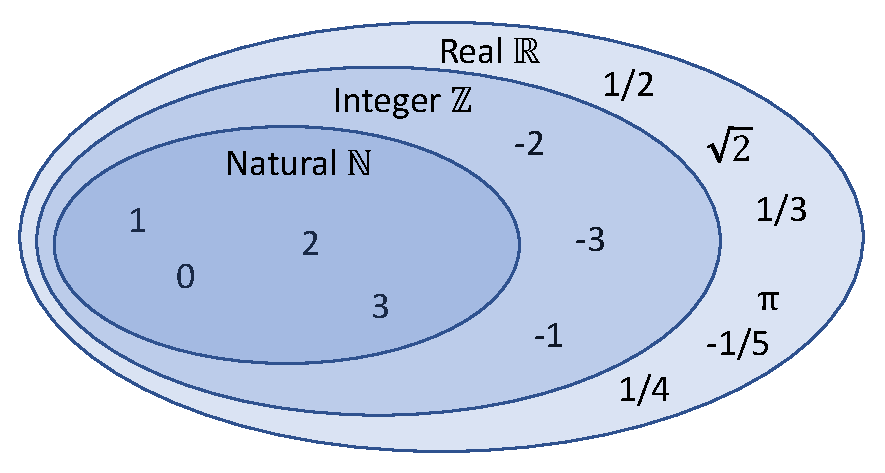
\includegraphics[width=0.6\textwidth]{numbers}
  \caption{In mathematics, the sets of natural, integer, and real numbers are each infinitely large, and real contains integers which in turn contains the set of natural numbers.}
  \label{fig:numbers}
\end{figure}
For many problems, working with infinite sets is impractical, and instead, a lot of work in the early days of the computer's history was spent on designing finite sets of numbers, which have many of the properties of their mathematical equivalent, but which also are efficient for performing calculations on a computer. For example, the set of integers in F\# is called \keyword{int} and is the set $\{\numprint{-2147483648} \ldots \numprint{2147483647}\}$.

Types are also important when programming. For example, a the \lstinline{string} \lstinline{"863"} and the \lstinline{int} \lstinline{863} may conceptually be identical but they are very different in the computer. F\# is very picky about types, and generally does not allow types to be mixed, as demonstrated in the interactive session in \Cref{typeInferenceError}.
%
\fsOutput{typeInferenceError}{Mixing types is often not allowed.}
%
In this example, we see that adding a string to an integer results in an error. The \idx{error message} contains much information. First, it illustrates where dotnet could not understand the input by \lstinline{------------^}. Then it repeats where the error is found as \lstinline[language=console]{/User/.../src/stdin(3,13)}, which means that \lstinline[language=console]{dotnet} was started in the directory \lstinline[language=console]{/User/.../src/}, the input was given on the standard-input meaning the keyboard, and the error was detected on line 3, column 13. Then  F\# gives the error number and a description of the error. Error numbers are an underdeveloped feature in F\# and should be ignored. However, the verbal description often contains useful information for correcting the program. Here, we are informed that there is a type mismatch in the expression. The reason for the mismatch is that since \lstinline{a} is an integer, then the \lexeme{+} operator must be integer addition, and thus for the expression to be executable, \lstinline{b} can only be an integer.

\section{Organizing often used code in functions}
\lstinline{printfn} is an example of a built-in function, and very often we wish to define our own. For example, in longer programs, some code needs to be used in several places and defining functions to \idx{encapsulate} such code can be a great advantage for reducing the length of code, debugging, and writing code, which is easier to understand by other programmers. A function is defined using a \keyword{let}-binding. For example, to define a function, which takes two integers as input and returns their sum, we write
%
\begin{codeNOutput}[label=sumFunction,
  top=-5pt,
  bottom=-5pt,
  left=-2pt,
  right=-2pt,
]{: Defining the function \lstinline{sum}}
\begin{lstlisting}
let sum x y =
  x + y
\end{lstlisting} 
\end{codeNOutput}
%
What this means is that we bind the name \lstinline{sum} as a function, which takes two arguments and adds them. Further, in the function, the arguments are locally referred to by the names \lstinline{x} and \lstinline{y}. Indentation determines which lines should be evaluated when the function is called, and in this case, there is only one. The value of the last expression evaluated in a function is its return value. Here there is only one expression \lstinline{x+y}, and thus, this function returns the value of the addition. This program does not do anything, since the function is neither called nor is its output used. However, we can modify \Cref{quickStartSum} to include it as shown in \Cref{quickStartSumFct}.
% 
\fs{quickStartSumFct}{Adding two integers with the use of a in-code defined function.}
%
The output is the same for the two programs, and the computation performed is almost the same. A step-by-step manner by replacement of the computation performed in line~\ref{quickStartSumFctA} is
\begin{quote}
  \lstinline{let c = sum 357 864} $\quad\rightsquigarrow\quad$  \lstinline{let c = 357 + 864}  $\quad\rightsquigarrow\quad$  \lstinline{let c = 1221}
\end{quote}
The main difference is that with the function \lstinline{sum} we have an independent unit, which can be reused elsewhere in the code.


\section{Asking the user for input}
The \lstinline{printfn} function allows us to write to the screen, which is useful, but sometimes we wish to start a dialogue with the user. One way to get user input is to ask the user to type something on the keyboard. Technically, input from the keyboard is called an \idx[stdin]{\lstinline{stdin}} \idx{stream}. This terminology is intended to remind us of characters streaming from the keyboard like the flow of water in a stream. Computer streams are different than water streams in that characters (or other items) only flow, when we ask for them. F\# provides many libraries of prebuilt functions, and here we will use the \lstinline{System.Console.ReadLine} function. The \lexeme{.}-lexeme is read as \lstinline{ReadLine} is a function which lies in \lstinline{Console} which in turn lies in \lstinline{System}. In the function documentation, we can read that \lstinline{System.Console.ReadLine} takes a unit value as an argument and returns the \idx[string]{\keyword{string}} the user typed. A string is a built-in type, as is integers, and strings contains sequences of characters. The program will not advance until the user presses the newline. An example of a program that multiplies two integers supplied by a user is given in \Cref{quickStartSumInput},
% 
\fs{quickStartSumInput}{Asking the user for input. The user entered \lstinline{6}, pressed the return button, \lstinline{2}, and pressed return again.}
%
In this program, we find a user dialogue, and we have designed it such that we assume that the user is unfamiliar with the inner workings of our program, and therefore helps the user understand the purpose of the input and the expected result. This is good programming practice. Here, we will not discuss the program line-to-line, but it is advised to the novice programmer to match what is printed on the screen and from where in the code, the output comes from. However, let us focus on line~\ref{quickStartSumInputA} and~\ref{quickStartSumInputA}, which introduce two new programming constructs. In each of these lines, 3 things happen: First the System.Console.ReadLine function is called with the \lexeme{()} value as argument. This reads all the characters, the user types, up until the user presses the return key. The return value is a string of characters such as \lstinline{"6"}. This value is different from the integer 6, and hence, to later be able to perform integer-addition, we \idx{cast} the string value to \keyword{int}, meaning that we call the function \keyword{int} to convert the string-value to the corresponding integer value. Finally, the result is bound to the names \lstinline{a} and \lstinline{b} respectively.


\section{Conditionally execute code}
Often problem requires code evaluated based on conditions, which only can be decided at \idx{runtime}, i.e., at the time, when the program is run. Consider a slight modification of our problem as
%
\begin{task}{probl:divisionInt}
  Ask for two interger values from the user, $a$ and $b$, and print the result of the integer division $a/b$.
\end{task}
%
To solve this problem, we must decide what to do, if the user inputs $b=0$, since division by zero is ill-defined. This is an example of a user input error, and later, we will investigate many different methods for handling such errors, but here, we will simply write an error message to the user, if the desired division is ill-defined. Thus, we need to decide at \idx{runtime}, whether to divide a and b or to write an error message. For this we will use the \keyword{match}-\keyword{with}\idxs{match@\keyword{match}}\idxs{with@\keyword{with}} expression.   
% 
\fs{quickStartDivisionInput}{Conditionally divide two user-given values.}
%
In this program, the \keyword{match}-\keyword{with} expression covers line~\ref{quickStartDivisionInputA} to~\ref{quickStartDivisionInputD}. When the computer executes these lines, it checks the value \lstinline{b} against a list of  patterns separated by \lexeme{|}. The code belonging to each pattern follows the arrow, \lexeme{->}, and is called a \idx{branch}, and which lines belongs to each branch is determined by \idx{indentation}. Hence, the code belonging to the \lexeme{0.0} branch is line~\ref{quickStartDivisionInputB} and to the \lexeme{_} branch is line~\ref{quickStartDivisionInputC} to~\ref{quickStartDivisionInputD}. The branches are checked one at a time from top to bottom. I.e., first \lstinline{b} is compared with \lstinline{0} which is equivalent to check whether \lstinline{b = 0.0}. If this is true, then its branch is executed. Otherwise, the \lstinline{b} is compared with the \idx{wildcard} pattern, \lexeme{_}. The wildcard pattern matches anything, and hence, if \lstinline{b} is nonzero, then \lexeme{_}-branch is executed. In most cases, F\# will give an error, if the list of patterns do not cover the full domain of the type being matched. Here, \lstinline{b} is an integer, and thus, we must write branches that takes \emph{all} integer values into account. The wildcard pattern makes this easy and works as a catch-all-other cases, and is often placed as the last case, following the important cases. Assuming that the user enters the value 0, then the step-by-step simplification of \keyword{match}-\keyword{with} expression is, 
\begin{quote}
  \lstinline{match b  with 0 -> ... | _ -> ...}\\ $\quad\rightsquigarrow\quad$ \lstinline{do printfn "Input error: Cannot divide by zero"}
\end{quote}

\section{Repeatedly execute code}
Often code needs to be evaluated many times or looped. For example, instead of stopping the program in \Cref{quickStartDivisionInput} if the user inputs $b=0$, then we could repeat the question as many times as needed until the user inputs a non-zero value for $b$. This is called a loop, and there are several programming constructions for this purpose.

Let us first consider recursion. A recursive function is one, which calls itself, e.g., $f(f(f(\dots(x))))$ is an example of a function $f$ which calls itself many times, possibly infinitely many. In the latter case, we say that the recursion has entered an infinite loop, and we will experience that either the program runs forever or that the execution stops due to a memory error. If we had infinite memory. To avoid this, recursive functions must always have a stopping criterion. Thus, we can design a function for asking the user for a non-zero input value as shown in \Cref{quickStartRecursiveInput}.
% 
\fs{quickStartRecursiveInput}{Recursively call \lstinline{ReadLine} until a non-zero value is entered.}
%
The function \lstinline{readNonZeroValue} takes no input denoted by \lexeme{()}, and repeatedly calls itself until the $a\neq 0$ condition is met. It is recursive since its body contains a call to itself. For technical reasons, F\# requires recursive functions to be declared by the \idx[rec]{\keyword{rec}}-keyword as demonstrated. The function has been designed to stop if $a\neq 0$, and in F\#, this is tested with the \lexeme{<>} operator. Thus, if the stopping condition is satisfied, then the \keyword{then}-branch is executed, which does not call itself, and thus the recursion goes no deeper. If the condition is not met, then the \keyword{else}-branch is executed, and the function is eventually called anew. The example execution of the program demonstrates this for the case that the user first inputs the value 0 and then the value 3.

As an alternative to recursive functions, loops may also be implemented using the \idx[while]{\keyword{while}}-expression. In \Cref{quickStartRecursiveInput} is an example of a solution where the recursive loop has been replaced with \keyword{while}-loop.
% 
\fs{quickStartWhileInput}{Replacing recursion in \Cref{quickStartRecursiveInput} with a \keyword{while}-loop.}
%
As for other constructs, the lines to be repeated are indicated by indentation, in this case, lines~\ref{quickStartWhileInputC} to~\ref{quickStartWhileInputD}, and in the end, the result of the
\lstinline{readNonZeroValueAlt} function is the last expression evaluated, which is the trivial expression \lstinline{a} in line~\ref{quickStartWhileInputE}. In comparison with the recursive version of the program, the \keyword{while}-loop has a continuation conditions (line~\ref{quickStartWhileInputB}), i.e., the content of the loop is repeated as long as \lstinline{a = 0} evaluates to \keyword{true}. Another difference is that in \Cref{quickStartRecursiveInput} we could simplify our program to only using \keyword{let} value-bindings, here we need a new concept: \idx[variable]{variables} also known as a \idx[mutable]{\keyword{mutable}} value. Mutable values allow us to update the value associated with a given name. Thus, the value associated with a name of mutable type depends on when it is accessed. This construction makes programs much more complicated and error-prone, and their use should be minimized. The syntax of mutable values is that first it should be defined with the \keyword{mutable}-keyword as shown in line~\ref{quickStartWhileInputA}, and when its value is to be updated then the \lexeme{<-}-notation must be used as demonstrated in line~\ref{quickStartWhileInputD}. Note that the execution of the two programs \Cref{quickStartRecursiveInput} and \Cref{quickStartWhileInput}, gives identical output, when presented with identical input. Hence, they solve the same problem by two quite different means. This is a common property of solutions to problems as a program: Often several different solutions exist, which are identical on the surface, but where the quality of the solution depends on how quality is defined and which programming constructions have been used. Here, the main difference is that the recursive solution avoids the use of mutable values, which turns out to be better for proving the correctness of programs and for adapting programs to super-computer architectures. However, recursive solutions may be very memory intensive, if the recursive call is anywhere but the last line of the function. 

\section{Programming as a form of communication}
When programming it is important to consider the time dimension of a program. Some usually very small programs are only used for a short while, e.g., to test a programming construction or an idea to a solution. Others small as well as large may be used again and again over a long period, and possibly given to other programmers to use, maintain, and extend. In this case, programming is an act of communication, where what is being communicated is the solution to a problem as well as the thoughts behind the chosen solution. Common experiences among programmers are that it is difficult to fully understand the thoughts behind a program written by a fellow programmer from its source code alone, and for code written perhaps just weeks earlier by the same programmer, said programmer can find it difficult to remember the reasons for specific programming choices. To support this communication, programmers use code-\idx{comments}. As a general concept, this is also called in-code documentation. Documentation may also be an accompanying manual or report. Documentation serves several purposes:
\begin{enumerate}
\item Communicate what the code should be doing, e.g., describe functions in terms of their input-output relation.
\item Highlight big insights essential for the code.
\item Highlight possible conflicts and/or areas where the code could be changed later.
\end{enumerate}
F\# has two different syntaxes for comments. A block comment is everything bracketed by \lstinline{(* *)}, and a line comment, which is everything between \lexeme{//} and the end of the line. For example, adding comments to \Cref{quickStartRecursiveInput} could look like \Cref{quickStartRecursiveInputComments}
% 
\fsCode{quickStartRecursiveInputComments}{quickStartRecursiveInputComments}{Adding comments to \Cref{quickStartRecursiveInput}.}{}
%
Comments are ignored by the computer and serve solely as programmer-to-programmer communication, there are no or few rules for specifying, what is good and bad documentation of a program. The essential point is that coding is a journey in problem-solving, and proper documentation is an aid in understanding the solution and the journey that lead to it.

\section{Key concepts and terms in this chapter}
\begin{itemize}
\item F\# has two modes of operation: \textbf{Interactive} and \textbf{compile} mode. The first chapters of this book will focus on the interactive mode. 
\item F\# is accessed through the \textbf{console/terminal/command-line}, which is another program, in which text commands can be given such as starting the dotnet program in interactive mode.
\item Programs are written in a human-readable form called the \textbf{source-code}.
\item Source code consists of several syntactical elements such as \textbf{operators} such as "*" and "<-", \textbf{keywords} such as "let" and "while", \textbf{values} such as 1.2 and the string "hello world", and \textbf{user-defined names} such as "a" and "str". All words, which F\# recognizes are called \textbf{lexemes}.
\item A program consists of a sequence of \textbf{expressions}, which comes in two types: \textbf{let} and \textbf{do}.
\item Values have \textbf{types} such as \textbf{int} and \textbf{string}. When performing calculations, the type defines which calculations can be done.
\item \textbf{Functions} are a type of value and defined using a let-binding. They are used to encapsulate code to make the code easier to read and understand and to make code reusable.
\item The \textbf{conditional} \textbf{match-with} expression is used to control what code is to be executed at \textbf{runtime}. Each piece of conditional code is called a \textbf{branch}
\item \textbf{Recursion} and \textbf{while}-loops are programming structure to execute the same code several times.
\item \textbf{Mutable values} are in contrast to \textbf{immutable values} may change value over time, and makes programmer harder to understand.
\item \textbf{Comments} are \textbf{in-code documentation} and are ignored by the computer but serve as an important tool for communication between programmers.
\end{itemize}

\end{document}


\documentclass[springer.tex]{subfiles}
\graphicspath{ {./figures/} }

\begin{document}
\chapter{Using F\# as a Calculator}
\label{chap:calculator}
%Talking about programs and programming languages we make a distinction between the language's \idx{syntax}, which describes what are legal expressions and statements, and the \idx{semantics} of an expression and a statement, which describes what is meant. This is analog to human languages, where how nouns, verbs, etc. may be placed in relation to each describes the syntax of a sentence, while the meaning of a sentence is its semantics. Basic elements of F\#'s syntax are literals, which is a fixed value like the number 3.
In this chapter, we will exclusively use the interactive mode to illustrate basic types and operations in F\#.

\section{Literals and Basic Types}
All programs rely on processing of data, and an essential property of data is its \idx{type}. A \idx{literal} is a fixed value like the number 3, and if we type the number \lstinline!3! in an interactive session at the input prompt, then F\# responds as shown in \Cref{firstType}.
%
\fsOutput{firstType}{Typing the number 3.}
%
What this means is that F\# has inferred the type to be \idx[int@\lstinline{int}]{\lstinline{int}} and bound it to the identifier \idx[it@\lstinline{it}]{\lstinline{it}}. For more on binding and identifiers see \Cref{chap:let}. Types matter, since the operations that can be performed on integers, are quite different from those that can be performed on, e.g., strings. Therefore, the number 3 has many different representations as shown in \Cref{typeMatters}.
%
\fsOutput{typeMatters}{Many representations of the number 3 but using different types.}
%
Each literal represents the number 3, but their types are different, and hence they are quite different values. The types \lstinline!int! for integer numbers, \idx[float@\lstinline{float}]{\lstinline{float}} for floating point numbers, \idx[bool@\lstinline{bool}]{\lstinline{bool}} for Boolean values, \idx[char@\lstinline{char}]{\lstinline{char}} for characters, and \idx[string@\lstinline{string}]{\lstinline{string}} for strings of characters are the most common types of literals. A table of all \idx{basic types} predefined in F\# is given in \Cref{tab:primitiveTypes}.\idxss{unit@\lstinline{unit}}\idxss{obj@\lstinline{obj}}\idxss{exn@\lstinline{exn}}
\begin{table}
  \centering
  \rowcolors{2}{oddRowColor}{evenRowColor}
  \begin{tabularx}{\textwidth}{|l|l|>{\raggedright\arraybackslash}X|}
    \hline
    \rowcolor{headerRowColor} Metatype & Type name & Description\\
    \hline
    Boolean & \underline{\keyword{bool}} & Boolean values true or false \\
    \hline
    Integer & \underline{\keyword{int}} & Integer values from -2,147,483,648 to 2,147,483,647 \\
             & \keyword{byte} &Integer values from 0 to 255\\
             & \keyword{sbyte} &Integer values from -128 to 127\\
             & \keyword{int8} &Synonymous with sbyte\\
             & \keyword{uint8} &Synonymous with byte\\
             & \keyword{int16} &Integer values from -32768 to 32767\\
             & \keyword{uint16} &Integer values from 0 to 65535\\
             & \keyword{int32} &Synonymous with int\\
             & \keyword{uint32} & Integer values from 0 to 4,294,967,295\\
             & \keyword{int64} &Integer values from -9,223,372,036,854,775,808 to 9,223,372,036,854,775,807\\
             & \keyword{uint64} &Integer values from 0 to 18,446,744,073,709,551,615\\
             %& bignum &Integer not limited to 64 bits\\
             %& nativeint &A native pointer as a signed integer\\
            % & unativeint &A native pointer as an unsigned integer\\
    \hline
    Real &\underline{\keyword{float}} & 64-bit IEEE 754 floating point value from $-\infty$ to $\infty$\\
             & \keyword{double} & Synonymous with float\\
             & \keyword{single} &A 32-bit floating point type\\
             & \keyword{float32} &Synonymous with single\\
             & \keyword{decimal} &A floating point data type that has at least 28 significant digits\\
    \hline
    Character &\underline{\keyword{char}} &Unicode character\\
             &\underline{\keyword{string}} & Unicode sequence of characters\\
    \hline
    None &\underline{\keyword{unit}} & The value ()\\
    \hline
    Object &\underline{\keyword{obj}} & An object\\
    \hline
    Exception &\underline{\keyword{exn}} & An exception\\
    \hline
  \end{tabularx}
  \caption{List of some of the basic types. The most commonly used types are underlined. For a description of integer see Appendix~\ref{sec:binary}, for floating point numbers see Appendix~\ref{sec:floatingPoint}, for ASCII and Unicode characters see Appendix~\ref{sec:characterSets}, for objects see \Cref{chap:oop}, and for exceptions see \Cref{chap:errors}.}
  \label{tab:primitiveTypes}
\end{table}
In addition to these built-in types, F\# is designed such that it is easy to define new types. 

Humans like to use the \idx{decimal number} system for representing numbers. Decimal numbers are \idx{base}~10, which means that a value is represented as two sequences of decimal digits separated by a \idx{decimal point}, where each \idx{digit} $d$ has a position and a value $d \in \{0,1,2,\ldots,9\}$. The part before the decimal point is called the \idx{whole part} and the part after is called the \idx{fractional part} of the number. An \idx{integer} is a number with only a whole part and neither a decimal point nor a fractional part. As an example \lstinline!35.7! is a decimal number, whose value is $3\cdot 10^1+5\cdot 10^0+7\cdot 10^{-1}$, and \lstinline!128! is an integer, whose value is $1\cdot 10^2+2\cdot 10^1+8\cdot 10^{0}$. In F\#, a decimal number is called a \idx{floating point number}.  Floating point numbers may alternatively be given using \idx{scientific notation}, such as \lstinline!3.5e-4! and \lstinline!4e2!, where the \lstinline!e!-notation is translated to a value as \lstinline!3.5e-4!~$=3.5\cdot 10^{-4} = 0.00035$, and \lstinline!4e2!~$=4\cdot 10^2=400$.

The basic unit of information in almost all computers is the binary digit or \idx{bit} for short. Internally, programs and data are all represented as bits, hence F\# has a strong support for binary numbers. A \idx{binary number} consists of a sequence of binary digits separated by a decimal point, where each digit can have values $b \in \{0,1\}$, and the base is $2$. E.g., the binary number $101.01_2 = 1\cdot 2^2+0\cdot 2^1+1\cdot 2^0+0\cdot 2^{-1}+1\cdot 2^{-2}=5.25$. Subscripts are often used to indicate the base of a number, e.g., $101.01_2$ and $101.01_{10}$ are different numbers. Since base 10 is so common, the subscript for base 10 numbers is often omitted. 

Binary numbers are closely related to \idx[octal number]{octal} and \idx[hexadecimal number]{hexadecimal numbers}. Octals uses 8 as basis and hexadecimals use 16 as basis. Each octal digit can be represented by exactly three bits, and each hexadecimal digit can represented by exactly four bits. The hexadecimal digits use \lstinline!0!--\lstinline!9! to represent the values 0--9 and \lstinline!a!--\lstinline!f! in lower or alternatively upper case to represent the values 10-15.  Thus, Octals and hexadecimals conveniently serve as shorthand for the much longer binary representation. As examples, the octal number \lstinline!37!$_8$ is $3\cdot 8^1+7\cdot 8^0=31$, and the hexadecimal number \lstinline!f3!$_{16}$ is $15\cdot 16^1+3\cdot 16^0=243$. 

To denote integers in bases different than 10, F\# uses the prefix '0b' for binary, '0o' for octal, and '0x' for hexadecimal numbers.  For example, the value $367_{10}$ may be written as an integer \lstinline!367!, as a binary number \lstinline!0b101101111!, as a octal number \lstinline!0o557!, and as a hexadecimal number \lstinline!0x16f!. In F\#, the character sequences \lstinline!0b12! and \lstinline!ff! are not recognized as numbers.

A \idx{character} is a \idx{Unicode} \idx{code point}, and character literals are enclosed in single quotation marks. Appendix~\ref{sec:unicode} contains more details on code points.\spec{Spec-4.0 p.28: \texttt{char-char} is missing option \texttt{unicodegraph-long} } The character type in F\# is denoted \idx[char@\lstinline{char}]{\keyword{char}}.  Examples of characters are 'a', 'D', '3', and examples of non-characters are '23' and 'abc'. Some characters, such as the tabulation character, do not have a visual representation. These can still be represented as a character using \idx{escape sequences}. A character escape sequence starts with \lexeme{\\} followed by letter for simple escapes such as \lstinline{\t} for tabulation and \lstinline{\n} for newline. Escape sequences can also be a numerical representation of a code point, and three versions exist: The trigraph \lstinline|\DDD|, where \lstinline{D} is a decimal digit, is used to specify the first 256 code points, the hexadecimal escape codes \lstinline|\uXXXX|, where \lstinline{X} is a hexadecimal digit, is used to specify the first 65536 code points, and \lstinline|\UXXXXXXXX| is used to specify any of the approximately $4.3\cdot 10^9$ possible code points. All escape sequences are shown in \Cref{tab:escapeChar}.
%
\begin{table}
  \centering
  \rowcolors{2}{oddRowColor}{evenRowColor}
  \begin{tabular}{|c|p{0.2\textwidth}|p{0.57\textwidth}|}
    \hline
    \rowcolor{headerRowColor} Character& Escape sequence & Description\\
    \hline
    BS &\lstinline|\b|& Backspace\\
    LF &\lstinline|\n|&Line feed\\
    CR &\lstinline|\r|&Carriage return\\
    HT &\lstinline|\t|&Horizontal tabulation\\
    \textbackslash &\lstinline|\\|&Backslash\\
     " &\lstinline|\"|&Quotation mark\\
    ' &\lstinline|\'|&Apostrophe\\
    BEL&\lstinline|\a|& Bell\\
    FF&\lstinline|\f|&Form feed\\
    VT &\lstinline|\v|&Vertical tabulation\\
    &\lstinline|\uXXXX|, \lstinline|\UXXXXXXXX|, \lstinline|\DDD|&Unicode character ('X' is any hexadecimal digit, and 'D' is any decimal digit)\\
    \hline
  \end{tabular}
  \caption{Escape characters. The escapecode \inlinecode{\textbackslash DDD} is sometimes called a tricode.}
  \label{tab:escapeChar}
\end{table}
%
Examples of \keyword{char} representations of the letter 'a' are: \lstinline{'a'}, \lstinline{'\097'}, \lstinline{'\u0061'}, \lstinline{'\U00000061'}.

A \idx{string} is a sequence of characters enclosed in double quotation marks.  Examples are \lstinline{"a"}, \lstinline{"this is a string"}, and \lstinline{"-&#\@"}. Note that the string \lstinline{"a"} and the character \lstinline{'a'} are not the same. Some strings are so common that they are given special names: One or more spaces \lstinline{" "} is called \idx{whitespace}, and both \lstinline{"\n"} and \lstinline{"\r\n"} are called \idx{newline}.  The escape-character \lexeme{\\} may be used to break a line in two. This and other examples are shown in \Cref{stringLiterals}.
%
\fsOutput{stringLiterals}{Examples of string literals.}
%
Note that the response from \lstinline[language=console]{fsharpi} is shown in double quotation marks, but this is not part of the string. 

F\# supports \idx[literal type]{literal types}, where the type of a literal is indicated as a prefix or suffix as shown in \Cref{tab:literalTypes}.\idxss{int32@\lstinline{int32}}\idxss{uint32@\lstinline{uint32}}\idxss{byte@\lstinline{byte}}\idxss{uint8@\lstinline{uint8}}\idxss{byte@\lstinline{byte[]}}\idxss{sbyte@\lstinline{sbyte}}\idxss{int8@\lstinline{int8}}\idxss{int16@\lstinline{int16}}\idxss{uint16@\lstinline{uint16}}\idxss{int64@\lstinline{int64}}\idxss{uint64@\lstinline{uint64}}\idxss{double@\lstinline{double}}\idxss{single@\lstinline{single}}\idxss{float32@\lstinline{float32}}\idxss{decimal@\lstinline{decimal}}
\begin{table}
  \centering
  %\begin{tabularx}{\linewidth}{|>{\hsize=.6\hsize}X|>{\hsize=1.4\hsize}X|>{\hsize=1\hsize}X|}
  \rowcolors{2}{oddRowColor}{evenRowColor}
  \setlength{\tabcolsep}{3pt}
  \begin{tabular}{|p{24mm}|p{25mm}|p{28mm}|p{27mm}|}
    \hline
    \rowcolor{headerRowColor} Type & syntax & Examples & Value \\
    \hline
    {\keyword{int}}, {\keyword{int32}}          
                                   & {\lstinline[language=syntax, keywords={}]!<*int | xint*>!}\newline
                                     {\lstinline[language=syntax, keywords={}]!<*int | xint*>l!}
                                            & {\lstinline!3!}, {\lstinline!0x3!}\newline
                                              {\lstinline!3l!}, {\lstinline!0x3l!}
                                                       & 3\\
    {\keyword{uint32}}                                 
                                   & {\lstinline[language=syntax, keywords={}]!<*int | xint*>u!}\newline
                                     {\lstinline[language=syntax, keywords={}]!<*int | xint*>ul!}
                                            & {\lstinline!3u!}\newline
                                              {\lstinline!3ul!}
                                                       & 3 \\
    {\keyword{byte}}, {\keyword{uint8}}       
                                   & {\lstinline[language=syntax, keywords={}]!<*int | xint*>uy!}\newline
                                     {\lstinline[language=syntax, keywords={}]!'<*char*>'B!}
                                            & {\lstinline!97uy!}\newline
                                                       {\lstinline!'a'B!} 
                                                       & 97 \\
    {\keyword{byte[]}}
                                   & {\lstinline[language=syntax, keywords={}]!"<*string*>"B!}\newline
                                     {\lstinline[language=syntax, keywords={}]!@"<*string*>"B!}
                                            & {\lstinline!"a\n"B!}\newline
                                                       {\lstinline!@"a\n"B!} 
                                                       & [|97uy; 10uy|]\newline
                                                         [|97uy; 92uy; 110uy|] \\
    {\keyword{sbyte}}, {\keyword{int8}}
                                   & {\lstinline[language=syntax, keywords={}]!<*int | xint*>y!}
                                            & {\lstinline!3y!}
                                                       & 3 \\
    {\keyword{int16}}
                                   & {\lstinline[language=syntax, keywords={}]!<*int | xint*>s!}
                                            & {\lstinline!3s!}
                                                       & 3 \\
    {\keyword{uint16}}
                                   & {\lstinline[language=syntax, keywords={}]!<*int | xint*>us!}
                                            & {\lstinline!3us!}
                                                       & 3 \\
    {\keyword{int64}}
                                   & {\lstinline[language=syntax, keywords={}]!<*int | xint*>L!}
                                            & {\lstinline!3L!}
                                                       & 3 \\
    {\keyword{uint64}}
                                   & {\lstinline[language=syntax, keywords={}]!<*int | xint*>UL!}\newline
                                     {\lstinline[language=syntax, keywords={}]!<*int | xint*>uL!}   
                                            & {\lstinline!3UL!}\newline
                                              {\lstinline!3uL!}  
                                                       & 3 \\
    % {\keyword{bignum}}$^*$                      & {\lstinline[language=syntax, keywords={}]!dInt "I"!}                                        & {\lstinline!3I!} & 3 \\
    % {\keyword{nativeint}}                            & {\lstinline[language=syntax, keywords={}]!(dInt | xInt) "n"!}                           & {\lstinline!3n!} & 3 \\
    % {\keyword{unativeint}}                          & {\lstinline[language=syntax, keywords={}]!(dInt | xInt) "un"!}                         & {\lstinline!3un!} & 3 \\
    {\keyword{float}}, {\keyword{double}}
                                   & {\lstinline[language=syntax, keywords={}]!<*float*>!}\newline
                                     {\lstinline[language=syntax, keywords={}]!<*xint*>LF!}
                                            & {\lstinline!3.0!}\newline
                                              {\lstinline!0x013LF!} 
                                                       & 3.0\newline
                                                         9.387247271e-323 \\
    {\keyword{single}}, {\keyword{float32}} 
                                   & {\lstinline[language=syntax, keywords={}]!<*float*>F!}\newline
                                     {\lstinline[language=syntax, keywords={}]!<*float*>f!}\newline
                                     {\lstinline[language=syntax, keywords={}]!<*xint*>lf!} 
                                   & {\lstinline!3.0F!}\newline
                                     {\lstinline!3.0f!}\newline
                                     {\lstinline!0x013lf!}
                                                       & 3.0\newline
                                                         3.0 \newline
                                                         4.4701421e-43f \\
    {\keyword{decimal}}  
                                   & {\lstinline[language=syntax, keywords={}]!<*float | int*>M!}\newline
                                     {\lstinline[language=syntax, keywords={}]!<*float | int*>m!}
                                            & {\lstinline!3.0M!}, {\lstinline!3M!}\newline
                                              {\lstinline!3.0m!}, {\lstinline!3m!} 
                                                       & 3.0  \\
    {\keyword{string}} 
                                   & {\lstinline[language=syntax, keywords={}]!"<*string*>"!}\newline
                                     {\lstinline[language=syntax, keywords={}]!@"<*string*>"!}\newline
                                     {\lstinline[language=syntax, keywords={}]!"""<*string*>"""!}
                                            & {\lstinline!"\"quote\".\n"!}\newline
                                              {\lstinline!@"""quote"".\n"!}\newline
                                              {\lstinline!""""quote".\n"""!}
                                                       & "quote".<newline>\newline
                                                         "quote".\textbackslash n.\newline
                                                         "quote".\textbackslash n\\
    \hline
  \end{tabular}
  % \end{tabularx}
  \caption{List of literal types. The syntax notation {\lstinline[language=syntax, keywords={}]!<**>!} means that the programmer replaces the brackets and content with a value of the appropriate form. The \lstinline[language=syntax, keywords={}]{<*xint*>} is one of the integers on hexadecimal, octal, or binary forms such as \lstinline{0x17}, \lstinline{0o21}, and \lstinline{0b10001}.  The \lstinline{[| |]} brackets means that the value is an array, see \Cref{sec:arrays} for details.
    % The \lstinline![]! notation is for lists, see \Cref{chap:lists}. $^*$\lstinline[language=ebnf]!bignum! is not a basic type and does not yet have an implementation for \lstinline[language=ebnf]!dInt ("Q"|"R"|"Z"|"N"|"G")! in Mono.
  }
  \label{tab:literalTypes}
\end{table}
%The table uses a simple syntax notation such that {\lstinline[language=syntax, keywords={}]!<*integer or hexadecimal*>UL!} means that the user supplies an integer or a hexadecimal number followed by the characters 'UL'.


The literal type is closely connected to how the values are represented internally. For example, a value of type \keyword{int32} use 32 bits and can be both positive and negative, while a \keyword{uint32} value also use 32 bits, but is unsigned. A \keyword{byte} is an 8-bit number, and \keyword{sbyte} is a signed 8-bit number. Values of type \keyword{float} use 64 bits, while \keyword{float32} only uses 32 bits. The number of bits used to represent numbers directly relates to the range and precession these types can represent. This is summarized in \Cref{tab:primitiveTypes} and discussed in more detail in \Cref{app:numbers}. String literals may be \idx{verbatim} by the @-notation or triple double quotation marks, meaning that the escape sequences are not converted to their code point. The two types of string verbatim treat quotation marks differently, as illustrated in the table. Further examples are shown in \Cref{namedLiterals}.
%
\fsOutput{namedLiterals}{Named and implied literals.}
%
%
%\fsOutput{stringVerbatim}{Examples of a string literal.}
%
%For strings containing double quotation marks, verbatim literals have 2 possible notations, either use the @-notation and escaping double quotation marks with an extra double quotation mark, or use triple double quotation marks. \advice{The triple double quotation marks notation may not contain substrings that are triple double quotation marks, and thus @-notation is preferred.}

Many basic types are compatible, and the type of a literal may be changed by \idx{typecasting}. An example of casting to a \keyword{float} is shown in \Cref{upcastingInt}.
%
\fsOutput{upcastingInt}{Casting an integer to a floating point number.}
% 
When \lstinline|float| is given an argument, then it acts as a function rather than a type, and for the integer \lstinline|3| it returns the floating point number \lstinline|3.0|.  For more on functions see \Cref{chap:let}. Boolean values are often treated as the integer values 0 and 1, but no short-hand function names exist for their conversions. Instead, use functions from the \lstinline{System.Convert} family of functions, as demonstrated in \Cref{castingBooleans}.
%
\fsOutput{castingBooleans}{Casting booleans.}
% 
Here \lstinline|System.Convert.ToBoolean| is the identifier of a function \lstinline|ToBoolean|, which is a \idx{member} of the \idx{class} \lstinline|Convert| that is included in the \idx{namespace} \lstinline|System|. Namespaces, classes, and members will be discussed in \Cref{chap:modules}.

Typecasting is often a destructive operation, e.g., typecasting a \lstinline!float! to \lstinline{int} removes the fractional part without rounding as shown in \Cref{downcasting}.
%
\fsOutput{downcasting}{Fractional part is removed by downcasting.}
%
Here we typecasted to a lesser type, in the sense that the set of integers is a subset of floating point numbers, and this is called \idx[downcast]{downcasting}. The opposite is called \idx[upcast]{upcasting} and is often non-destructive, as \Cref{upcastingInt} showed. Since floating point numbers are a superset of integers, the value is retained. As a side note, \idx{rounding} a number $y.x$, where $y$ is the \idx{whole part} and $x$ is the \idx{fractional part}, is the operation of mapping numbers in the interval $y.x \in [y.0,y.5)$ to $y$, and those in $y.x\in [y.5,y+1)$ to $y+1$. This can be performed by downcasting, as shown in \Cref{rounding}.
%
\fsOutput{rounding}{Rounding by modified downcasting.}
%
I.e., $357.6+0.5=358.1$ and removing the fractional part by downcasting results in $358$, which is the correct answer.

\section{Operators on Basic Types}
Expressions are the basic building block of all F\# programs, and this section will discuss operator expressions on basic types. 
A typical calculation, such used in \Cref{rounding}, is \begin{equation}
  \underbrace{357.6}_{\text{operand}}\quad\underbrace{+}_{\text{operator}}\quad\underbrace{0.5}_{\text{operand}}
\end{equation}
is an example of an arithmetic \idx{expression}, and the above expression consists of two \idx[operand]{operands} and an \idx{operator}. Since this operator takes two operands, it is called a \idx{binary operator}. The expression is written using \idx{infix notation}, since the operands appear on each side of the operator.

In order to discuss general programming structures, we will use a simplified language to describe valid syntactical structures. In this simplified language, the syntax of basic binary operators is shown in the following.
%
\begin{verbatimwrite}{\ebnf/binaryOperator.ebnf}
<*expr*><*op*><*expr*>
\end{verbatimwrite}
\syntax{\ebnf/binaryOperator.ebnf}{Syntax for a binary expression.}
%
Here \lstinline[language=syntax]{<*expr*>} is any expression supplied by the programmer, and \lstinline[language=syntax]{<*op*>} is a binary infix operator. F\# supports a range of arithmetic binary infix operators on its built-in types, such as addition, subtraction, multiplication, division, and exponentiation, using the \lexeme{+}, \lexeme{-}, \lexeme{*}, \lexeme{/}, \lexeme{**} lexemes, respectively. Not all operators are defined for all types, e.g., addition is defined for integer and float types as well as for characters and strings, but multiplication is only defined for integer and floating-point types. A complete list of built-in operators on basic types is shown in \Cref{tab:preNInfixOperators} and~\ref{tab:comparisonOperators}, and a range of mathematical functions is shown in \Cref{tab:arithmeticFunctions}.
%
\begin{table}
  \centering
  \rowcolors{2}{oddRowColor}{evenRowColor}
  \begin{tabularx}{\linewidth}{|c|c|c|c|c|c|l|l|>{\raggedright\arraybackslash}X|}
    \hline
    \rowcolor{headerRowColor} \rotatebox{90}{Operator} & \rotatebox{90}{\lstinline!bool!}& \rotatebox{90}{\lstinline!ints!}& \rotatebox{90}{\lstinline!floats!}& \rotatebox{90}{\lstinline!char!}& \rotatebox{90}{\lstinline!string!} & Example & Result &Description\\
    \hline
    \lstinline!+!& & \checkmark & \checkmark & \checkmark & \checkmark & \lstinline!5 + 2!&\lstinline!7!&Addition\\
    \hline
    \lstinline!-!& & \checkmark & \checkmark & & & \lstinline!5.0 - 2.0!&\lstinline!3.0!&Subtraction\\
    \hline
    \lstinline!*!& & \checkmark & \checkmark & & & \lstinline!5 * 2!&\lstinline!10!&Multiplication\\
    \hline
    \lstinline!/!& & \checkmark & \checkmark & & & \lstinline!5.0 / 2.0!&\lstinline!2.5!&Division\\
    \hline
    \lstinline!\%!& & \checkmark & \checkmark & & & \lstinline!5 \% 2!&\lstinline!1!&Remainder\\
    \hline
    \lstinline!**!& & & \checkmark & & & \lstinline!5.0 ** 2.0!&\lstinline!25.0!&Exponentiation\\
    \hline
    \lstinline!+!& & \checkmark & \checkmark & & &\lstinline!+3!&\lstinline!3!&identity\\
    \hline
    \lstinline!-!& & \checkmark & \checkmark & & &\lstinline!-3.0!&\lstinline!-3.0!&negation\\
    \hline
    \lstinline!\&\&!& \checkmark & & & & & \lstinline!true \&\& false!&\lstinline!false!&boolean and\\
    \hline
    \lstinline!||!& \checkmark & & & & & \lstinline!true || false!&\lstinline!true!&boolean or\\
    \hline
    \lstinline!not!& \checkmark & & & & &\lstinline!not true!&\lstinline!false!&boolean negation\\
    \hline
    \lstinline!\&\&\&!& & \checkmark & & & & \lstinline!0b101 \&\&\& 0b110!&\lstinline!0b100!&bitwise boolean and\\
    \hline
    \lstinline!|||!& & \checkmark & & & & \lstinline!0b101 ||| 0b110!&\lstinline!0b111!&bitwise boolean or\\
    \hline
    \lstinline!\^\^\^!& & \checkmark & & & & \lstinline!0b101 \^\^\^ 0b110!&\lstinline!0b011!&bitwise boolean exclusive or\\
    \hline
    \lstinline!<<<!& & \checkmark & & & & \lstinline!0b110uy <<< 2!&\lstinline!0b11000uy!&bitwise left shift\\
    \hline
    \lstinline!>>>!& & \checkmark & & & & \lstinline!0b110uy >>> 2!&\lstinline!0b1uy!&bitwise right shift\\
    \hline
    \lstinline!\~\~\~!& & \checkmark & & &&\lstinline!\~\~\~0b110uy!&\lstinline!0b11111001uy!&bitwise boolean negation\\
    \hline
  \end{tabularx}
  \caption{Arithmetic operators on basic types. Ints and floats means all built-in integer and float types. Note that for the bitwise operations, digits \lstinline{0} and \lstinline{1} are taken to be \lstinline{true} and \lstinline{false}.}
  \label{tab:preNInfixOperators}
\end{table}
%
\begin{table}
  \centering
  \rowcolors{2}{oddRowColor}{evenRowColor}
  \begin{tabularx}{\linewidth}{|c|c|c|c|c|c|l|l|X|}
    \hline
    \rowcolor{headerRowColor} \rotatebox{90}{Operator} & \rotatebox{90}{\lstinline!bool!}& \rotatebox{90}{\lstinline!ints!}& \rotatebox{90}{\lstinline!floats!}& \rotatebox{90}{\lstinline!char!}& \rotatebox{90}{\lstinline!string!} & Example & Result &Description\\
    \hline
    \lstinline!<!& \checkmark & \checkmark & \checkmark & \checkmark & \checkmark & \lstinline!true < false!&\lstinline!false!&Less than\\
    \hline
    \lstinline!>!& \checkmark & \checkmark & \checkmark & \checkmark & \checkmark & \lstinline!5 > 2!&\lstinline!true!&Greater than\\
    \hline
    \lstinline!=!& \checkmark & \checkmark & \checkmark & \checkmark & \checkmark & \lstinline!5.0 = 2.0!&\lstinline!false!&Equal\\
    \hline
    \lstinline!<=!& \checkmark & \checkmark & \checkmark & \checkmark & \checkmark & \lstinline!'a' <= 'b'!&\lstinline!true!&Less than or equal\\
    \hline
    \lstinline!>=!& \checkmark & \checkmark & \checkmark & \checkmark & \checkmark & \lstinline!"ab" >= "cd"!&\lstinline!false!&Greater than or equal\\
    \hline
    \lstinline!<>!& \checkmark & \checkmark & \checkmark & \checkmark & \checkmark & \lstinline!5 <> 2!&\lstinline!true!&Not equal\\
    \hline
  \end{tabularx}
  \caption{Comparison operators on basic types. Types cannot be mixed, e.g., \lstinline!3<'a'! is a syntax error.}
  \label{tab:comparisonOperators}
\end{table}
\idxss{\lstinline{abs}}\idxss{\lstinline{acos}}\idxss{\lstinline{asin}}\idxss{\lstinline{atan}}\idxss{\lstinline{atan2}}\idxss{\lstinline{ceil}}\idxss{\lstinline{cos}}\idxss{\lstinline{cosh}}\idxss{\lstinline{exp}}\idxss{\lstinline{floor}}\idxss{\lstinline{log}}\idxss{\lstinline{log10}}\idxss{\lstinline{max}}\idxss{\lstinline{min}}\idxss{\lstinline{pown}}\idxss{\lstinline{round}}\idxss{\lstinline{sign}}\idxss{\lstinline{sin}}\idxss{\lstinline{sinh}}\idxss{\lstinline{sqrt}}\idxss{\lstinline{tan}}\idxss{\lstinline{tanh}}
%
\begin{table}
  \centering
  \begin{tabularx}{\linewidth}{|c|c|c|c|c|c|l|l|>{\raggedright\arraybackslash}X|}
    \hline
    \rowcolor{headerRowColor} \rotatebox{90}{Operator} & \rotatebox{90}{\lstinline!bool!}& \rotatebox{90}{\lstinline!ints!}& \rotatebox{90}{\lstinline!floats!}& \rotatebox{90}{\lstinline!char!}& \rotatebox{90}{\lstinline!string!} & Example & Result &Description\\
    \hline
    \lstinline!abs! & & \checkmark & \checkmark & & &\lstinline!abs -3! & \lstinline!3! & Absolute value\\
    \hline 
    \lstinline!acos! & & & \checkmark & & &\lstinline!acos 0.8! & \lstinline!0.644! & Inverse cosine\\
     \hline 
     \lstinline!asin! & & & \checkmark & & & \lstinline!asin 0.8! & \lstinline!0.927! & Inverse sinus\\
     \hline 
     \lstinline!atan! & & & \checkmark & & & \lstinline!atan 0.8! & \lstinline!0.675! & Inverse tangent\\
     \hline 
     \lstinline!atan2! & & & \checkmark & & & \lstinline!atan2 0.8 2.3! & \lstinline!0.335! & Inverse tangentvariant\\
     \hline 
     \lstinline!ceil! & & & \checkmark & & & \lstinline!ceil 0.8! & \lstinline!1.0! & Ceiling\\
     \hline 
     \lstinline!cos!   & & & \checkmark & & & \lstinline!cos 0.8! & \lstinline!0.697! & Cosine\\
     \hline 
 %  \lstinline!cosh!   & & & \checkmark & & & \lstinline!cosh 0.8! & \lstinline!1.34! & Hyperbolic cosine\\
 %    \hline 
     \lstinline!exp! & & & \checkmark & & & \lstinline!exp 0.8! & \lstinline!2.23! & Natural exponent\\
     \hline 
     \lstinline!floor! & & & \checkmark & & & \lstinline!floor 0.8! & \lstinline!0.0! & Floor\\
     \hline 
     \lstinline!log! & & & \checkmark & & & \lstinline!log 0.8! & \lstinline!-0.223! & Natural logarithm\\
     \hline 
     \lstinline!log10! & & & \checkmark & & & \lstinline!log10 0.8! & \lstinline!-0.0969! & Base-10 logarithm\\
     \hline 
     \lstinline!max! & & \checkmark & \checkmark & \checkmark & \checkmark & \lstinline!max 3.0 4.0! & \lstinline!4.0! & Maximum\\
     \hline 
     \lstinline!min! & & \checkmark & \checkmark & \checkmark & \checkmark & \lstinline!min 3.0 4.0! & \lstinline!3.0! & Minimum\\
     \hline 
     \lstinline!pown! & & \checkmark & & & & \lstinline!pown 3 2! & \lstinline!9! & Integer exponent\\
     \hline 
     \lstinline!round! & & & \checkmark & & & \lstinline!round 0.8! & \lstinline!1.0! & Rounding\\
     \hline 
     \lstinline!sign!  & & \checkmark & \checkmark & & & \lstinline!sign -3! & \lstinline!-1! & Sign\\
     \hline 
     \lstinline!sin! & & & \checkmark & & & \lstinline!sin 0.8! & \lstinline!0.717! & Sinus\\
     \hline 
 %  \lstinline!sinh! & & & \checkmark & & & \lstinline!sinh 0.8! & \lstinline!0.888! & Hyperbolic sinus\\
 %    \hline 
     \lstinline!sqrt! & & & \checkmark & & & \lstinline!sqrt 0.8! & \lstinline!0.894! & Square root\\
     \hline 
     \lstinline!tan! & & & \checkmark & & & \lstinline!tan 0.8! & \lstinline!1.03! & Tangent\\
     \hline 
 %   \lstinline!tanh! & & & \checkmark & & & \lstinline!tanh 0.8! & \lstinline!0.664! & Hyperbolic tangent\\
 %    \hline 
  \end{tabularx}
  \caption{Predefined functions for arithmetic operations.}
  \label{tab:arithmeticFunctions}
\end{table}
%
Note that expressions can themselves be arguments to expressions, and thus, \lstinline!4+5+6! is also a legal statement. Technically, F\# interprets the expression as \lstinline!(4+5)+6! meaning that first \lstinline!4+5! is evaluated according the \lstinline[language=syntax]{<*expr*><*op*><*expr*>} syntax. Then the result replaces the parenthesis to yield \lstinline!9+6!, which, once again, is evaluated according to the \lstinline[language=syntax]{<*expr*><*op*><*expr*>} syntax to give \lstinline!15!.  This is called \idx{recursion}, which is the name for a type of rule or function that uses itself in its definition. See \Cref{sec:recursion} for more on recursive functions.

Unary operators take only one argument and have the syntax:
%
\begin{verbatimwrite}{\ebnf/unaryOperator.ebnf}
<*op*><*expr*>
\end{verbatimwrite}
\syntax{\ebnf/unaryOperator.ebnf}{A unary expressions.}
%
An example of a unary operator is \lstinline!-3!, where \lstinline!-! here is used to negate a positive integer. Since the operator appears before the operand, it is a \idx{prefix operator}. 

The concept of \idx{precedence} is an important concept in arithmetic expressions.\jon{minor comment on indexing and slice-ranges.} If parentheses are omitted in \Cref{rounding}, then F\# will interpret the expression as \lstinline|(int 357.6)  + 0.5|, which is erroneous since the addition of an integer with a float is undefined. This is an example of precedence, i.e., function evaluation takes precedence over addition which means that function evaluation is performed first and addition second. Consider the arithmetic expression shown in \Cref{simpleArithmetic}.
%
\fsOutput{simpleArithmetic}{A simple arithmetic expression.}
%
Here, the addition and multiplication functions are shown in infix notation with the \idx{operator} lexemes \lexeme{+} and \lexeme{*}. To arrive at the resulting value 23, F\# has to decide in which order to perform the calculation. There are 2 possible orders, \lstinline|3 + (4 * 5)| and \lstinline|(3 + 4) * 5| that gives different results. For integer arithmetic, the correct order is, of course, multiplication before addition, and we say that multiplication takes \idx{precedence} over addition. Every atomic operation that F\# can perform is ordered in terms of its precedence, and for some common built-in operators shown in \Cref{tab:someOperatorPrecedences}, the precedence is shown by the order they are given in the table.
\begin{table}
  \newlength{\myl}
  \setlength{\myl}{\widthof{\lstinline[language=syntax]|<*expr*> \^\^\^ <*expr*>|}+3em}
  \centering
  \rowcolors{2}{oddRowColor}{evenRowColor}
  \begin{tabularx}{\linewidth}{|l|l|X|}
    \hline
    \rowcolor{headerRowColor} Operator & Associativity & Description\\
    \hline
    \begin{minipage}[t]{\the\myl}\lstinline[language=syntax]|+<*expr*>|\\\lstinline[language=syntax]|-<*expr*>|\\\lstinline[language=syntax]|\~\~\~<*expr*>|\end{minipage} & Left & Unary identity, negation, and bitwise negation operators\\
    \hline
    \begin{minipage}[t]{\the\myl}\lstinline[language=syntax]|f <*expr*>|\end{minipage} & Left & Function application\\
    \hline
    \begin{minipage}[t]{\the\myl}\lstinline[language=syntax]|<*expr*> ** <*expr*>|\end{minipage} & Right & Exponentiation\\ 
    \hline
    \begin{minipage}[t]{\the\myl}\lstinline[language=syntax]|<*expr*> * <*expr*>|\\\lstinline[language=syntax]|<*expr*> / <*expr*>|\\\lstinline[language=syntax]|<*expr*> \% <*expr*>|\end{minipage} & Left & Multiplication, division and remainder\\
    \hline
    \begin{minipage}[t]{\the\myl}\lstinline[language=syntax]|<*expr*> + <*expr*>|\\\lstinline[language=syntax]|<*expr*> - <*expr*>|\end{minipage} & Left & Addition and subtraction binary operators\\
    \hline
    \begin{minipage}[t]{\the\myl}\lstinline[language=syntax]|<*expr*> \^\^\^ <*expr*>|\end{minipage} & Right & Bitwise exclusive or\\
    \hline
    \begin{minipage}[t]{\the\myl}\lstinline[language=syntax]|<*expr*> < <*expr*>|\\\lstinline[language=syntax]|<*expr*> <= <*expr*>|\\\lstinline[language=syntax]|<*expr*> > <*expr*>|\\\lstinline[language=syntax]|<*expr*> >= <*expr*>|\\\lstinline[language=syntax]|<*expr*> = <*expr*>|\\\lstinline[language=syntax]|<*expr*> <> <*expr*>|\\\lstinline[language=syntax]|<*expr*> \<\<\< <*expr*>|\\\lstinline[language=syntax]|<*expr*> >>> <*expr*>|\\\lstinline[language=syntax]|<*expr*> \&\&\& <*expr*>|\\\lstinline[language=syntax]!<*expr*> ||| <*expr*>!\end{minipage}
             & Left & Comparison operators, bitwise shift, and bitwise 'and' and 'or'.\\
    \hline
    \begin{minipage}[t]{\the\myl}\lstinline[language=syntax]|<*expr*> \&\& <*expr*>|\end{minipage} & Left & Boolean and\\
    \hline
    \begin{minipage}[t]{\the\myl}\lstinline[language=syntax]+<*expr*> || <*expr*>+\end{minipage} & Left & Boolean or\\
    \hline
  \end{tabularx}
  \caption{Some common operators, their precedence, and their associativity. Rows are ordered from highest to lowest precedences, such that \lstinline|<*expr*> * <*expr*>| has higher precedence than \lstinline|<*expr*> + <*expr*>|. Operators in the same row have the same precedence..}
  \label{tab:someOperatorPrecedences}
\end{table}

Associativity describes the order in which calculations are performed for binary operators of the same precedence. Some operator's associativity are given in \Cref{tab:someOperatorPrecedences}. In the table we see that \lexeme{*} is left associative, which means that \lstinline{3.0 * 4.0 * 5.0} is evaluated as \lstinline{(3.0 * 4.0) * 5.0}. Conversely, \lstinline{**} is right associative, so \lstinline{4.0**3.0**2.0} is evaluated as \lstinline{4.0**(3.0**2.0)}. For some operators, like multiplication, association matters little, e.g., $4*3*2=4*(3*2)=(4*3)*2$, and for other operators, like exponentiation, association makes a huge difference, e.g., $4^{(3^2)}\neq (4^3)^2$. Examples of this is shown in \Cref{precedence}.\spec{Spec-4.0, Table 18.2.1 appears to be missing Boolean 'and' and 'or' operations. Section 4.4 seems to be missing \&\&\& and ||| bitwise operators.}
%
\fsOutput{precedence}{Precedence rules define implicit parentheses.}
%
\advice{Whenever in doubt of association or any other basic semantic rules, it is a good idea to use parentheses. It is also a good idea to test your understanding of the syntax and semantic rules by making a simple script.}%

\section{Boolean Arithmetic}
Boolean arithmetic is the basis of almost all computers and particularly important for controlling program flow, which will be discussed in \Cref{chap:flow}. Boolean values are one of 2 possible values, true or false, which is also sometimes written as 1 and 0. Basic operations on Boolean values are '\idx{and}', '\idx{or}', and '\idx{not}', which in F\# are written respectively as the binary operators \lstinline!&&!, \lstinline!||!, and the function \lstinline!not!. Since the domain of Boolean values is so small, all possible combination of input on these values can be written on the tabular form, known as a \idx{truth table}, and the truth tables for the basic Boolean operators and functions are shown in \Cref{tab:truthTable}.
\begin{table}
  \centering
  \rowcolors{2}{oddRowColor}{evenRowColor}
  \begin{tabular}{|c|c|c|c|c|}
    \hline
    \rowcolor{headerRowColor} \lstinline!a! & \lstinline!b! & \lstinline!a && b!& \lstinline!a || b! & \lstinline!not a!\\
    \hline
    \lstinline!false!&\lstinline!false!&\lstinline!false!&\lstinline!false!&\lstinline!true!\\
    \lstinline!false!&\lstinline!true!&\lstinline!false!&\lstinline!true!&\lstinline!true!\\
    \lstinline!true!&\lstinline!false!&\lstinline!false!&\lstinline!true!&\lstinline!false!\\
    \lstinline!true!&\lstinline!true!&\lstinline!true!&\lstinline!true!&\lstinline!false!\\
    \hline
  \end{tabular}
  \caption{Truth table for boolean 'and', 'or', and 'not' operators. Value 0 is false and 1 is true.}
  \label{tab:truthTable}
\end{table}
A good mnemonic for remembering the result of the 'and' and 'or' operators is to use 1 for true, 0 for false, multiplication for the Boolean 'and' operator, and addition for the Boolean 'or' operator, e.g., true and false in this mnemonic translates to $1\cdot 0 = 0$, and the result translates back to the Boolean value false. In F\#, the truth table for the basic Boolean operators can be produced by a program, as shown in \Cref{truthTable}.
%
\fsOutput{truthTable}{Boolean operators and truth tables.}
%
Here, we used the \lstinline|printfn| function to present the results of many expressions on something that resembles a tabular form. The spacing produced using the \lstinline|printfn| function is not elegant, and in \Cref{sec:printf} we will discuss better options for producing more beautiful output. Notice that the arguments for \lstinline|printfn| was given on the next line with indentation. The indentation is an important part of telling F\# which part of what you write belong together. This is an example of the so-called lightweight syntax. Generally, F\# ignores newlines and whitespaces except when using the lightweight syntax. The difference between verbose and lightweight syntax is discussed in \Cref{chap:let}.

\section{Integer Arithmetic}
The set of integers is infinitely large, but since all computers have limited resources, it is not possible to represent it in its entirety. The various integer types listed in \Cref{tab:primitiveTypes} are finite subsets reduced by limiting their ranges. 
%Although \lstinline!bignum! is theoretically unlimited, the biggest number representable is still limited by computer memory. 
An in-depth description of integer implementation can be found in \Cref{app:numbers}. The type \keyword{int} is the most common type. 

\Cref{tab:preNInfixOperators,tab:comparisonOperators,tab:arithmeticFunctions} give examples of operators and functions pre-defined for integer types. Notice that fewer functions are available for integers than for floating point numbers. For most addition, subtraction, multiplication, and negation, the result is straightforward. However, performing arithmetic operations on integers requires extra care, since the result may cause \idx{overflow} and \idx{underflow}. For example, an \lstinline|sbyte| is specified using the \lexeme{y}-literal and can hold values $[-128\ldots 127]$. This causes problems in the example in \Cref{overflow}.
%
\fsOutput{overflow}{Adding integers may cause overflow.}
%
Here $100+30=130$, which is larger than the biggest \lstinline|sbyte|, and the result is an overflow. Similarly, we get an underflow, when the arithmetic result falls below the smallest value storable in an \lstinline|sbyte|, as demonstrated in \Cref{underflow}.
%
\fsOutput{underflow}{Subtracting integers may cause underflow.}
%
I.e., we were expecting a negative number but got a positive number instead.

The overflow error in \Cref{overflow} can be understood in terms of the binary representation of integers: In binary, $130=10000010_2$, and this binary pattern is interpreted differently as \lstinline{byte} and \lstinline{sbyte}, see \Cref{overflowBits}.
%
\fsOutput{overflowBits}{The leftmost bit is interpreted differently for signed and unsigned integers, which gives rise to potential overflow errors.}
%
That is, for signed bytes, the left-most bit is used to represent the sign, and since the addition of $100=01100100_2$ and $30=00011110_b$ is $130=10000010_2$, which causes the left-most bit to be used, this is wrongly interpreted as a negative number when stored in an \lstinline{sbyte}. Similar arguments can be made explaining underflows.

The \idxs{integer division} operator discards the fractional part after division, and the \idx{integer remainder} operator calculates the remainder after integer division, as demonstrated in \Cref{integerDivisionRemainder}.
%
\fsOutput{integerDivisionRemainder}{Integer division and remainder operators.}
%
Together, the integer division and remainder can form a lossless representation of the original number, see \Cref{integerDivisionRemainderLossless}.
%
\fsOutput{integerDivisionRemainderLossless}{Integer division and remainder is a lossless representation of an integer, compare with \Cref{integerDivisionRemainder}.}
%
Here we see that integer division of 7 by 3 followed by multiplication by 3 is less than 7, and that the difference is \lstinline!7 % 3!.

Notice that neither overflow nor underflow error gave rise to an error message, which is why such bugs are difficult to find. 
 Dividing any non-zero number by 0 is infinite, which is also outside the domain of any of the integer types, but in this case, F\# casts an \idx{exception}, as shown in \Cref{integerDivisionByZeroError}.
%
\fsOutput{integerDivisionByZeroError}{Integer division by zero causes an exception runtime error.}
%
The output looks daunting at first sight, but the first and last lines of the error message are the most important parts, which tell us what exception was cast and why the program stopped. The middle contains technical details concerning which part of the program caused the error and can be ignored for the time being. Exceptions are a type of \idx{runtime error}, and are discussed in \Cref{chap:errors}

Integer exponentiation is not defined as an operator but is available as the built-in function \lstinline|pown|. This function is demonstrated in \Cref{integerPown} for calculating $2^5$.
%
\fsOutput{integerPown}{Integer exponent function.}
%

For binary arithmetic on integers, the following operators are available:
\lstinline[language=syntax]{<*leftExpr*> <<< <*rightExpr*>}, which shifts the bit pattern of \lstinline[language=syntax]|<*leftExpr*>| \lstinline[language=syntax]|<*rightExpr*>| positions to the left while inserting 0's to right;
\lstinline[language=syntax]{<*leftExpr*> >>> <*rightExpr*>}, which shifts the bit pattern of \lstinline[language=syntax]|<*leftExpr*>| \lstinline[language=syntax]|<*rightExpr*>| positions to the right while inserting 0's to left; 
\lstinline[language=syntax]{~~~ <*expr*>} returns a new integer, where all 0 bits are changed to 1 bits and vice-versa;
\lstinline[language=syntax]{<*expr*> &&& <*expr*>} returns the result of taking the Boolean 'and' operator position-wise;
\lstinline[language=syntax]{<*expr*> ||| <*expr*>}  returns the result of taking the Boolean 'or' operator position-wise; and
\lstinline[language=syntax]{<*expr*> ^^^ <*expr*>} returns the result of the Boolean 'xor' operator defined by the truth table in \Cref{tab:xor}.\idxs{xor}\idxs{exclusive or}
\begin{table}
  \centering
  \rowcolors{2}{oddRowColor}{evenRowColor}
  \begin{tabular}{|c|c|c|}
    \hline
    \rowcolor{headerRowColor} \lstinline!a! & \lstinline!b! & \lstinline!a ^^^ b!\\
    \hline
    \lstinline!false! & \lstinline!false! & \lstinline!false!\\
    \lstinline!false! & \lstinline!true! & \lstinline!true!\\
    \lstinline!true! & \lstinline!false! & \lstinline!true!\\
    \lstinline!true! & \lstinline!true! & \lstinline!false!\\
    \hline
  \end{tabular}
  \caption{Boolean exclusive or truth table.}
  \label{tab:xor}
\end{table}
% Unfortunately, there are no built-in functions to output integers on binary form, so to understand the output of the following program,
% \begiverbatimwrite}{\ebnf/tmp.ebnf}
% > let a = 0b11000011uy  
% - let b = a <<< 1
% - let c = a >>> 1
% - let d = ~~~a
% - let e = a ^^^0b11111111uy;;
%
% val a : byte = 195uy
% val b : byte = 134uy
% val c : byte = 97uy
% val d : byte = 60uy
% val e : byte = 60uy
% \end{verbatimwrite}
%\ebnf{tmp.ebnf}{to do.}
% we must consider the 8-bit binary form of the unsigned integers: $195 = 11000011_2$, $134 = 10000110_2$, $97 = 01100001_2$, and $60 = 00111100_2$, which agrees with the definitions. 

\section{Floating Point Arithmetic}
Like integers, the set of reals is also infinitely large, hence, floating point types are finite subsets reduced by sampling the space of reals. An in-depth description of floating point implementations can be found in Appendix~\ref{app:numbers}. The type \keyword{float} is the most common type. 

\Cref{tab:preNInfixOperators,tab:comparisonOperators,tab:arithmeticFunctions} give examples of operators and functions pre-defined for floating point types. Note that the remainder operator for floats calculates the remainder after division and discards the fractional part, see \Cref{floatDivisionRemainder}.
%
\fsOutput{floatDivisionRemainder}{Floating point division and remainder operators.}
%
The remainder for floating point numbers can be fractional, but division, discarding fractional part, and the remainder is still a lossless representation of the original number, as demonstrated in \Cref{floatDivisionRemainderLossless}.
% 
\fsOutput{floatDivisionRemainderLossless}{Floating point division, downcasting, and remainder is a lossless representation of a number.}
%

Arithmetic using \lstinline|float| will not cause over- and underflow problems, since the IEEE 754 standard includes the special numbers $\pm\infty$ and NaN. As shown in \Cref{floatDivisionByZero}, no exception is thrown.
%
\fsOutput{floatDivisionByZero}{Floating point numbers include infinity and Not-a-Number.}
%
However, the \lstinline|float| type has limited precision, since there is only a finite number of numbers that can be stored in a float. E.g., addition and subtraction can give surprising results, as demonstrated in \Cref{floatImprecission}.
%
\fsOutput{floatImprecission}{Floating point arithmetic has finite precision.}
%
That is, addition and subtraction associates to the left, hence the expression is interpreted as \lstinline!(357.8 + 0.1)  - 357.9! and we see that we do not get the expected 0. The reason is that the calculation is done stepwise, and in the process, the numbers are represented using the imprecise floating point standard. Thus,\lstinline!357.8 + 0.1!  is represented as a number close to but not identical to what \lstinline!357.9! is represented as, and thus, when subtracting these two representations, we get a very small nonzero number. Such errors tend to accumulate, and comparing the result of expressions of floating point values should, therefore, be treated with care. Thus, \advice{equivalence of two floating point expressions should only be considered up to sufficient precision, e.g., comparing \lstinline!357.8 + 0.1! and \lstinline!357.9! up to \lstinline!1e-10! precision should be tested as, \lstinline!abs ((357.8 + 0.1) - 357.9)  < 1e-10!.}

\section{Char and String Arithmetic}
Addition is the only operator defined for characters. Nevertheless, character arithmetic is often done by casting to an integer. A typical example is the conversion of character case, e.g., to convert the lowercase character 'z' to uppercase. Here, we use the \idx{ASCIIbetical order}, add the difference between any Basic Latin Block letters in upper- and lowercase as \lstinline{integers}, and cast back to \lstinline{char}, see \Cref{upcaseChar}.
%
\fsOutput{upcaseChar}{Converting case by casting and integer arithmetic.}
%
I.e., the code point difference between upper and lower case for any alphabetical character 'a' to 'z' is constant, hence we can change case by adding or subtracting the difference between any corresponding character. Unfortunately, this does not generalize to characters from other languages.

A large collection of operators and functions exist for \lstinline{string}. The simplest is concatenation using the \lexeme{+} operator, as demonstrated in \Cref{stringConcatenation}.
%
\fsOutput{stringConcatenation}{Example of string concatenation.}
%
Characters and strings cannot be concatenated, which is why the above example used the string of a space \lstinline|" "| instead of the space character \lstinline|' '|. The characters of a string may be indexed as using the \idx[{.[]}@\lstinline{.[]}]{\lstinline{.[]}} notation. This is demonstrated in \Cref{stringIndexing}.
%
\fsOutput{stringIndexing}{String indexing using square brackets.}
%
Notice that the first character has index 0, and to get the last character in a string, we use the string's \lstinline{length} property. This is done as shown in \Cref{stringIndexingLength}.
%
\fsOutput{stringIndexingLength}{String length attribute and string indexing.}
%
Since index counting starts at 0, and since the string length is 7, the index of the last character is 6. 
%An alternative notation for indexing is to use the property \lstinline|Char|, and in the example \lstinline|''abcdefg''.[3]| is the same as \lstinline|a.Char 3|. 
There is a long list of built-in functions in \lstinline|System.String| for working with strings, some of which will be discussed in \Cref{sec:strings}.
 
The \idx{dot notation} is an example of Structured programming, where technically speaking, the string \mbox{\lstinline|"abcdefg"|} is an immutable \idx{object} of \idx{class} \lstinline|string|, \lstinline|[]| is an object \idx{method}, and \lstinline|Length| is a property. For more on objects, classes, and methods, see \Cref{chap:oop}.  

Strings are compared letter by letter. For two strings to be equal, they must have the same length and all the letters must be identical. E.g., \mbox{\lstinline!"abs" = "absalon"!} is false, while \lstinline!"abs" = "abs"! is true. The \lexeme{<>} operator is the boolean negation of the \lexeme{=} operator, e.g., \lstinline!"abs" <> "absalon"! is true, while \lstinline!"abs" <> "abs"! is false. For the \lexeme{<} , \lexeme{<=}, \lexeme{>}, and \lexeme{>=} operators, the strings are ordered alphabetically, such that \lstinline!"abs" < "absalon" && "absalon" < "milk"! is true, that is, the \lexeme{<} operator on two strings is true if the left operand should come before the right when sorting alphabetically. The algorithm for deciding the boolean value of \lstinline!leftOp < rightOp! is as follows: we start by examining the first character, and if \lstinline!leftOp.[0]! and \lstinline!rightOp.[0]! are different, then \lstinline!leftOp < rightOp! is equal to \lstinline!leftOp.[0] < rightOp.[0]!. E.g., \lstinline!"milk" < "abs"! is the same as \lstinline!'m' < 'a'!, which is false, since the letter 'm' does not come before the letter 'a' in the alphabet, or more precisely, the codepoint of 'm' is not less than the codepoint of 'a'. If \lstinline!leftOp.[0]! and \lstinline!rightOp.[0]! are equal, then we move on to the next letter and repeat the investigation, e.g., \lstinline!"abe" < "abs"! is true, since \lstinline!"ab" = "ab"! is true and \lstinline!'e' < 's'! is true. If we reach the end of either of the two strings, then the shorter word is smaller than the longer word, e.g., \lstinline!"abs" < "absalon"! is true, while \lstinline!"abs" < "abs"! is false. The \lexeme{<=}, \lexeme{>}, and \lexeme{>=} operators are defined in a similar manner.

\clearpage

\section{Tuples}
\idx[tuple]{Tuples} are a direct extension of constants. They are immutable and have neither concatenations nor indexing operations. Tuples are unions of immutable types and have the following syntax:
%
\begin{verbatimwrite}{\ebnf/tuples.ebnf}
<*expr*>{*, <*expr*>*}
\end{verbatimwrite}
\syntax{\ebnf/tuples.ebnf}{Tuples are list of expressions separated by commas.}
%
Tuples are identified by the \lexeme{,} lexeme and often enclosed in parentheses, but that is not required. An example is a triple, also known as a 3-tuple, \lstinline!(2,true,"hello")!. In interactive mode, the type of tuples is demonstrated in \Cref{tuple}.
%
\fsOutput{tuple}{Tuple types are products of sets.}
%
The values \lstinline!2!, \lstinline!true!, and \lstinline!"hello"! are \idx[member]{members}, and the number of elements of a tuple is its \idx{length}. From the response of F\#, we see that the tuple is inferred to have the type \lstinline!int * bool * string!. The \lexeme{*} denotes the Cartesian product between sets.  Tuples can be products of any types and follow the lexical scope rules like value and function bindings. Notice also that a tuple may be printed as a single entity by the \lstinline!%A! %
placeholder. In the example we bound \lstinline!tp! to the tuple. The opposite is also possible, as demonstrated in \Cref{tupleDeconstruction}.
%
\fsOutput{tupleDeconstruction}{Definition of a tuple.}
%
In this example, a function is defined that takes 1 argument, a 3-tuple. If we wanted a function with 3 arguments, then the function binding should have been \lstinline{let deconstructNPrint a b c = ...}. The value binding \lstinline{let (a, b, c) = tp}, binds a tuple with 3 named members to a value, thus deconstructing it in terms of its members. This is called pattern matching and will be discussed in further details in \Cref{chap:patterns}. Since we used the \lstinline!\%A! placeholder in the \lstinline!printfn! function, the function can be called with 3-tuples of different types. F\# informs us that the tuple type is variable by writing \lstinline{'a * 'b * 'c}. The \lexeme{'} notation means that the type can be decided at run-time, see \Cref{sec:variableTypes} for more on variable types. 

Pairs or 2-tuples are so common that F\# includes two built-in functions,\idx[fst@\lstinline{fst}]{\keyword{fst}} and \idx[snd@\lstinline{snd}]{\keyword{snd}}, to extract the first and second element of a pair. This is demonstrated in \Cref{pair}.
%
\fs{pair}{Deconstruction of pairs with the built-in functions \keyword{fst} and \keyword{snd}.}
%

Tuples of equal lengths can be compared, and the  comparison is defined similarly to string comparison. Tuples of equal length are compared element by element. E.g., \lstinline!(1,2) = (1,3)! is false, while \lstinline!(1,2) = (1,2)! is true. The \lexeme{<>} operator is the boolean negation of the \lexeme{=} operator. For the \lexeme{<} , \lexeme{<=}, \lexeme{>}, and \lexeme{>=} operators, the strings are ordered lexicographically, such that \lstinline!('a', 'b', 'c') < ('a', 'b', 's') && ('a', 'b', 's') <  ('c', 'o', 's')! is true, that is, the \lexeme{<} operator on two tuples is true if and only if the left operand should come before the right when sorting alphabetically. See \Cref{tupleCompare} for an example.
%
\fs{tupleCompare}{Tuples comparison is similar to string comparison.}
%
The algorithm for deciding the boolean value of \lstinline!(a1, a2) < (b1, b2)! is as follows: we start by examining the first elements, and if \lstinline!a1! and \lstinline!b1! are different, then the result of \lstinline!(a1, a2) < (b1, b2)! is equal to the result of \lstinline!a1 < b1!. If \lstinline!a1! and \lstinline!b1! are equal, then we move on to the next letter and repeat the investigation. The \lexeme{<=}, \lexeme{>}, and \lexeme{>=} operators are defined similarly.

Binding tuples to mutables does not make the tuple mutable. This is demonstrated in \Cref{tupleOfMutables}.
%
\fs{tupleOfMutables}{A mutable changes value, but the tuple defined by it does not refer to the new value.}
%
However, it is possible to define a mutable variable of type tuple such that new tuple values can be assigned to it, as shown in \Cref{mutableTuple}.
%
\fs{mutableTuple}{A mutable tuple can be assigned a new value.}
%
Mutable tuples are value types, meaning that binding to new names makes copies, not aliases, as demonstrated in \Cref{mutableTupleValue}.
%
\fs{mutableTupleValue}{A mutable tuple is a value type.}
%
The use of tuples shortens code and highlights semantic content at a higher level, e.g., instead of focusing on the elements, tuples focus on their union. While this may look elegant and short there is the risk of \idx{obfuscation}, i.e., writing compact code that is difficult to read, where an unprepared reader of the code may not easily understand the computation nor appreciate its elegance without an accompanying explanation.  Hence, \advice{always keep an eye out for compact and concise ways to write code, but never at the expense of readability.}

\section{Programming Intermezzo: Hand Conversion Between Decimal and Binary Numbers}
Conversion of integers between decimal and binary form is a key concept one must grasp in order to understand some of the basic properties of calculations on the computer. Converting from binary to decimal is straightforward if using the power-of-two algorithm, i.e., given a sequence of $n+1$ binary digits $b_i$ written as $b_n b_{n-1}\dots b_0$, and where $b_n$ and $b_0$ are the most and least significant bits respectively, then the decimal value is calculated as,
\begin{align}
  v = \sum_{i=0}^nb_i2^i
\end{align}
For example, $10011_2 = 1+2+16 = 19$. Converting from decimal to binary is a little more complex, but a simple divide-by-two algorithm exists. The key to understanding the divide-by-two algorithm is to realize that dividing a number by two is equivalent to shifting its binary representation one position to the right. E.g., $10 = 1010_2$ and $10/2 = 5 = 101_2$. Odd numbers have $b_0=1$, e.g., $11_{10} = 1011_2$ and $11_{10}/2 = 5.5 = 101.1_2$. Hence, if we divide any number by two and get a non-integer number, then its least significant bit was $1$. Another way to express this is to say that the least significant bit is the remainder after integer division by two. Sequential application of this idea leads directly to the divide-by-two algorithm. E.g., if we were to convert the number $11_{10}$ in decimal form to binary form, we would perform the following steps:
\begin{align*}
  11\tikzmark{a1} \text{ div } 2 = \tikzmark{a2}5\tikzmark{a3},\;   \tikzmark{a4}11  \text{ rem }  2 & =\tikzmark{a5}1\tikzmark{a6}\\
  \nonumber \\
  5\tikzmark{b1} \text{ div }  2 = \tikzmark{b2}2\tikzmark{b3},\;  \tikzmark{b4}5  \text{ rem } 2 & =\tikzmark{b5}1\tikzmark{b6}\\
  \\\nonumber
  2\tikzmark{c1}  \text{ div }  2 = \tikzmark{c2}1\tikzmark{c3},\;   \tikzmark{c4}2 \text{ rem }  2 & =\tikzmark{c5}0\tikzmark{c6} \\
  \\\nonumber
  1\tikzmark{d1}  \text{ div }  2 = \tikzmark{d2}0\tikzmark{d3},\;   \tikzmark{d4}1  \text{ rem }  2 & =\tikzmark{d5}1\tikzmark{d6}\\
\end{align*}%
\DrawArrow[]{a2}{b1}%
\DrawArrow[]{a3}{b4}%
\DrawArrow[]{b2}{c1}%
\DrawArrow[]{b3}{c4}%
\DrawArrow[]{c2}{d1}%
\DrawArrow[]{c3}{d4}%
\FrameArea{a5}{d6}%
\hspace*{-0.6mm}Here we used div and rem to signify the integer division and remainder operators. The algorithm stops when the result of integer division is zero. Reading off the remainder from below and up, we find the sequence $1011_2$, which is the binary form of the decimal number $11_{10}$. Using the interactive mode, we can perform the same calculation, as shown in \Cref{conversionByHand}.
\begin{codeNOutput}[label=conversionByHand]{: Converting the number $11_{10}$ to binary form.}
\begin{lstlisting}[language=console]
> printfn "(%d, %d)" (11 / 2) (11 % 2);;
(5, 1)
val it : unit = ()
> printfn "(%d, %d)" (5 / 2) (5 % 2);;  
(2, 1)
val it : unit = ()
> printfn "(%d, %d)" (2 / 2) (2 % 2);;  
(1, 0)
val it : unit = ()
> printfn "(%d, %d)" (1 / 2) (1 % 2);;
(0, 1)
val it : unit = ()
\end{lstlisting}
\end{codeNOutput}
Thus, by reading the second integer-response from \lstinline!printfn! from below and up, we again obtain the binary form of $11_{10}$ to be $1011_2$. For integers with a fractional part, the divide-by-two algorithm may be used on the whole part, while multiply-by-two may be used in a similar manner on the fractional part.
\end{document}


\chapter{Values and Functions}
\label{chap:let}
%
In this chapter, we will see how we can bind expressions to identifiers either as new constants, functions, or operators, how this saves time when building large programs, and how this makes programs easier to read and debug. As an example, consider the following problem,
\begin{problem}
  For given set constants $a$, $b$, and $c$, solve for $x$ in
  \begin{equation}
  a x^2+bx+c = 0
\end{equation}
\end{problem}
To solve for $x$ we use the quadratic formula from elementary algebra,
\begin{equation}
  x = \frac{-b\pm\sqrt{b^2-4ac}}{2a},
\end{equation}
which gives the general solution for any values of the coefficients. Here, we will assume a positive discriminant, $b^2-4ac>0$. In order to write a program where the code may be reused later, we define a function \mbox{\lstinline!discriminant : float -> float -> float -> float!}, that is, a function that takes 3 arguments, \lstinline!a!, \lstinline!b!, and \lstinline!c!, and calculates the discriminant. Likewise, we will define \mbox{\lstinline!positiveSolution : float -> float -> float -> float!} and \mbox{\lstinline!negativeSolution : float -> float -> float -> float!}, that also take the polynomial's coefficients as arguments and calculate the solution corresponding to choosing the positive and negative sign for $\pm$ in the equation. Details on function definition is given in \Cref{sec:functions}. Our solution thus looks like \Cref{identifiersExample}.
%
\fs{identifiersExample}{Finding roots for quadratic equations using function name binding.}
%
Here, we have further defined names of values \lstinline!a!, \lstinline!b!, and \lstinline!c! which are used as inputs to our functions, and the results of function application are bound to the names \lstinline!d!, \lstinline!xn!, and \lstinline!xp!. The names of functions and values given here are examples of identifiers, and with these, we may reuse the quadratic formulas and calculated values later, while avoiding possible typing mistakes and reducing the amount of code which needs to be debugged.

The use of identifiers is central in programming. For F\#, not to be confused with built-in functionality, identifiers must follow a specific set of rules: 
\begin{description} 
\item[Identifier]\idxs{identifier}~\\[-5mm]
  \begin{itemize}
  \item Identifiers are used as names for values, functions, types etc.
  \item They must start with a Unicode letter or underscore '\_', but can be followed by zero or more of letters, digits, and a range of special characters except for SP, LF, and CR (space, line feed, and carriage return). See \Cref{sec:unicode} for more on codepoints that represents letters. 
  \item They can also be a sequence of identifiers separated by a period.
  \item They cannot be keywords, see \Cref{tab:keywords}.
  \end{itemize}
\end{description}
\begin{table}
  \centering
  \rowcolors{2}{oddRowColor}{evenRowColor}
  \begin{tabularx}{\textwidth}{|l|>{\raggedright\arraybackslash}X|}
    \hline
    \rowcolor{headerRowColor} Type & Keyword\\
    \hline
  Regular 
  &\mbox{\lstinline{abstract},} \mbox{\lstinline{and},} \mbox{\lstinline{as},} \mbox{\lstinline{assert},} \mbox{\lstinline{base},} \mbox{\lstinline{begin},} \mbox{\lstinline{class},} \mbox{\lstinline{default},} \mbox{\lstinline{delegate},} \mbox{\lstinline{do},} \mbox{\lstinline{done},} \mbox{\lstinline{downcast},} \mbox{\lstinline{downto},} \mbox{\lstinline{elif},} \mbox{\lstinline{else},} \mbox{\lstinline{end},} \mbox{\lstinline{exception},} \mbox{\lstinline{extern},} \mbox{\lstinline{false},} \mbox{\lstinline{finally},} \mbox{\lstinline{for},} \mbox{\lstinline{fun},} \mbox{\lstinline{function},} \mbox{\lstinline{global},} \mbox{\lstinline{if},} \mbox{\lstinline{in},} \mbox{\lstinline{inherit},} \mbox{\lstinline{inline},} \mbox{\lstinline{interface},} \mbox{\lstinline{internal},} \mbox{\lstinline{lazy},} \mbox{\lstinline{let},} \mbox{\lstinline{match},} \mbox{\lstinline{member},} \mbox{\lstinline{module},} \mbox{\lstinline{mutable},} \mbox{\lstinline{namespace},} \mbox{\lstinline{new},} \mbox{\lstinline{null},} \mbox{\lstinline{of},} \mbox{\lstinline{open},} \mbox{\lstinline{or},} \mbox{\lstinline{override},} \mbox{\lstinline{private},} \mbox{\lstinline{public},} \mbox{\lstinline{rec},} \mbox{\lstinline{return},} \mbox{\lstinline{sig},} \mbox{\lstinline{static},} \mbox{\lstinline{struct},} \mbox{\lstinline{then},} \mbox{\lstinline{to},} \mbox{\lstinline{true},} \mbox{\lstinline{try},} \mbox{\lstinline{type},} \mbox{\lstinline{upcast},} \mbox{\lstinline{use},} \mbox{\lstinline{val},} \mbox{\lstinline{void},} \mbox{\lstinline{when},} \mbox{\lstinline{while},} \mbox{\lstinline{with},} and \mbox{\lstinline{yield}.}\\
 Reserved
 & \mbox{\lstinline{atomic},} \mbox{\lstinline{break},} \mbox{\lstinline{checked},} \mbox{\lstinline{component},} \mbox{\lstinline{const},} \mbox{\lstinline{constraint},} \mbox{\lstinline{constructor},} \mbox{\lstinline{continue},} \mbox{\lstinline{eager},} \mbox{\lstinline{fixed},} \mbox{\lstinline{fori},} \mbox{\lstinline{functor},} \mbox{\lstinline{include},} \mbox{\lstinline{measure},} \mbox{\lstinline{method},} \mbox{\lstinline{mixin},} \mbox{\lstinline{object},} \mbox{\lstinline{parallel},} \mbox{\lstinline{params},} \mbox{\lstinline{process},} \mbox{\lstinline{protected},} \mbox{\lstinline{pure},} \mbox{\lstinline{recursive},} \mbox{\lstinline{sealed},} \mbox{\lstinline{tailcall},} \mbox{\lstinline{trait},} \mbox{\lstinline{virtual},} and \mbox{\lstinline{volatile}.}\\
 Symbolic
 & \mbox{\lstinline{let!},} \mbox{\lstinline{use!},} \mbox{\lstinline{do!},} \mbox{\lstinline{yield!},} \mbox{\lstinline{return!},} \mbox{\lstinline{|},} \mbox{\lstinline{->},} \mbox{\lstinline{<-},} \mbox{\lstinline{.},} \mbox{\lstinline{:},} \mbox{\lstinline{(},} \mbox{\lstinline{)},} \mbox{\lstinline{[},} \mbox{\lstinline{]},} \mbox{\lstinline{[<},} \mbox{\lstinline{>]},} \mbox{\lstinline{[|},} \mbox{\lstinline{|]},} \mbox{\lstinline{\{},} \mbox{\lstinline{\}},} \mbox{\lstinline{'},} \mbox{\lstinline{#},} \mbox{\lstinline{:?>},} \mbox{\lstinline{:?},} \mbox{\lstinline{:>},} \mbox{\lstinline{..},} \mbox{\lstinline{::},} \mbox{\lstinline{:=},} \mbox{\lstinline{;;},} \mbox{\lstinline{;},} \mbox{\lstinline{=},} \mbox{\lstinline{_},} \mbox{\lstinline{?},} \mbox{\lstinline{??},} \mbox{\lstinline{(*)},} \mbox{\lstinline{<@},} \mbox{\lstinline{@>},} \mbox{\lstinline{<@@},} and \mbox{\lstinline{@@>}.} \\
 Reserved symbolic
 &\mbox{\lstinline{\~}} and \mbox{\lstinline{`}}\\
    \hline
  \end{tabularx}
  \caption{Table of (possibly future) \emph{keywords}\idxss{keyword} and symbolic keywords in F\#.}
  \label{tab:keywords}
\end{table}
Examples of identifiers are: \lstinline{a}, \lstinline{theCharacter9}, \lstinline{Next_Word}, \lstinline{_tok}, and \lstinline{f.sharp.rocks}.  Since programmers often work in multilingual environment dominated by the English language it is advicable to \advice{restrict identifiers to use letters from the English alphabet, numbers, period, and '\_'.}  However, the number of possible identifiers is enormous. The full definition refers to the Unicode general categories described in Appendix~\ref{sec:unicode}, and there are currently 19.345 possible Unicode code points in the letter category and 2.245 possible Unicode code points in the special character category.

Identifiers may be used to carry information about their intended content and use, and careful selection of identifiers can aid programmers to communicate thoughts about the code. Thus, identifiers are often a word or several concatenated words conveying some relevant meaning. For example, in the function definition \lstinline{let discriminant a b c = b ** 2.0 - 4.0 * a * c}, the function identifier has been chosen to be \lstinline{discriminant}. F\# places no special significance to the word 'discriminant', and the program would work exactly the same had the function been called \lstinline{let f a b c = b ** 2.0 - 4.0 * a * c}. However, to programmers, the word 'discriminant' informs us of the intended role of the function and thus is much preferred. This is a general principle: \advice{identifier names should be chosen to reflect their semantic value.}. The arguments \lstinline{a}, \lstinline{b}, and \lstinline{c} are short, but adheres to a textbook tradition of elementary algebra. Again, we might as well have used, \lstinline{let discriminant c a b = a ** 2.0 - 4.0 * c * b}, which is semantically identical to the original expression, but due to tradition, this would confuse most readers of the code. Thus, \advice{identifier names should be chosen consistently with the readers' traditions.} Finally, identifiers are often concatenations of words, as \lstinline{positiveSolution} in \Cref{identifiersExample}. Concatenations can be difficult to read. Without the capitalization of the second word, we would have had \lstinline{positivesolution}. This is readable at most times, but takes longer time to understand in general. Typical solutions are to use a separator, such as \lstinline{positive_solution}, \idx{lower camel case} also known as \idx{mixed case} as in the example \lstinline{positiveSolution}, and \idx{upper camel case} also known as \idx{pascal case} as \lstinline{PositiveSolution}. In this book, we use lower camel case except where F\# requires a capital first letter. Again, the choice does not influence what a program does, only how readable it is to a fellow programmer. The important part is that \advice{identifier names consisting of concatenated words are often preferred over names with few character, and concatenation should be emphasized, e.g., by camel casing.} Choosing the length of identifier names is a balancing act, since when working with large programs, very long identifier names can be tiresome to write, and a common practice is that the length of identifier names is proportional to the complexity of the program. I.e., complex programs use long names, simple programs use short names. What is complex and what is simple is naturally in the eye of the beholder, but when you program, remember that a future reader of the program most likely has not had time to work with the problem as long as the programmer, thus \advice{choose identifier names as if you were to explain the meaning of a program to a knowledgeable outsider.}

Another key concept in F\# is expressions. An expression can be a mathematical expression, such as $3*5$, a function application, such as $f 3$, and many other things. Central in this chapter is the binding of values and functions to identifiers, which is done with the keyword \keyword{let}, e.g., \lstinline!let a = 1.0!.

Expressions are the main workhorse of F\# and have an enormous variety in how they may be written. We will in this book gradually work through some of the more important facets.
\begin{description} 
\item[Expressions]\idxs{expression}~\\[-5mm]
  \begin{itemize}
  \item An Expression is a computation such as \lstinline{3 * 5}.
  \item They can be value bindings between identifiers and expressions that evaluate to a value or a function, see \Cref{sec:values,sec:functions}.
  \item They can be \lstinline{do}-bindings that produce side-effects and whose result are ignored, see \Cref{sec:functions} 
  \item They can be assignments to variables, see \Cref{sec:values}.
  \item They can be a sequence of expressions separated with the \idx[;@\lstinline{;}]{\lexeme{;}} lexeme.
  \item They can be annotated with a type by using the \idx[:@\lstinline{:}]{\lexeme{:}} lexeme.
  \end{itemize}
\end{description}

Before we begin a deeper discussion on bindings, note that F\#  adheres to two different syntaxes: \idx[verbose syntax]{verbose} and \idx[lightweight syntax]{lightweight}. In the verbose syntax, newlines and whitespaces are generally ignored, while in lightweight syntax, certain keywords and lexemes may be replaced by newlines and whitespaces. The lightweight syntax is the most common, but the syntaxes may be mixed, and we will highlight the options, when relevant.

\section{Value Bindings}
\label{sec:values}
Binding identifiers to literals, or expressions that are evaluated to be values, is called \idx{value-binding}, and examples are \lstinline!let a = 3.0! and \lstinline!let b = cos 0.9!. Value bindings have the following syntax:
%
\begin{verbatimwrite}{\ebnf/valueBindings.ebnf}
let <*valueIdent*> = <*bodyExpr*> [*in <*expr*>*]
\end{verbatimwrite}
\syntax{\ebnf/valueBindings.ebnf}{Value binding expression.}
%
The \idx[let@\lstinline{let}]{\keyword{let}} keyword binds a value-identifier \lstinline[language=syntax]{<*valueIdent*>} with an expression \lstinline[language=syntax]{<*bodyExpr*>} that evaluates to a value. The following square bracket notation \lstinline[language=syntax]{[**]} means that the enclosed is optional, and F\# is able to identify whether or not the optional part is used by whether or not the \idx[in@\lstinline{in}]{\keyword{in}} keyword is present in the binding expression. If the \keyword{in} keyword is used, then the value-identifier is a local definition in the following \lstinline[language=syntax]{<*expr*>} expression but in the following lines. For lightweight syntax, the \keyword{in} keyword is replaced with a newline, and the binding \emph{is} valid in the following lines at the level of scope of the value-binding, or deeper, lexically.

The value identifier annotated with a type by using the \idx[:@\lstinline{:}]{\lexeme{:}} lexeme followed by the name of a type, e.g., \lstinline{int}. The \idx[\_@\lstinline{_}]{\lexeme{\_}} lexeme may be used as a value-identifier. This lexeme is called the \idx{wildcard pattern}, and for value-bindings it means that \lstinline[language=syntax]{<*bodyExpr*>} is evaluated, but the result is discarded. See \Cref{chap:patterns} for more details on patterns.

For example, letting the identifier \lstinline!p! be bound to the value \lstinline!2.0! and using it in an expression is done as shown in \Cref{letValue}.
%
\fs{letValue}{The identifier \lstinline!p! is used in the expression following the \keyword{in} keyword.}
%
F\# will ignore most newlines between lexemes, i.e., the above is equivalent to writing as shown in \Cref{letValueLF}.
%
\fs{letValueLF}{Newlines after \keyword{in} make the program easier to read.}
%
F\# also allows for an alternative notation called \idx{lightweight syntax}, where e.g., the \keyword{in} keyword is replaced with a newline, and the expression starts on the next line at the same column as \keyword{let} starts in, i.e., the above is equivalent to \Cref{letValueLightWeight}.
%
\fs{letValueLightWeight}{Lightweight syntax does not require the \keyword{in} keyword, but the expression must be aligned with the \keyword{let} keyword.}
%
The same expression in interactive mode will also show with the inferred types, as shown in \Cref{letValueLightWeightTypes}.
%
\fsOutput{letValueLightWeightTypes}{Interactive mode also outputs inferred types.}
%
By the \keyword{val} keyword in the line \lstinline!val p : float = 2.0!, we see that \lstinline!p! is inferred to be of type \lstinline!float! and bound to the value \lstinline!2.0!. The inference is based on the type of the right-hand-side which is \lstinline!float!.  Identifiers may be defined to have a type using the \lexeme{:} lexeme, but the types on the left-hand-side and right-hand-side of the \lexeme{=} lexeme must be identical. Mixing types gives an error, as shown in \Cref{letValueTypeError}.
%
\fs{letValueTypeError}{Binding error due to type mismatch.}
% \begin{lstlisting}[language=fsharp,caption={fsharpi, binding error due to type mismatch.}]
%   > let a : float = 3;;
%
%   let a : float = 3;;
%   ----------------^
%
% /Users/sporring/repositories/fsharpNotes/stdin(50,17): error FS0001: This expression was expected to have type
%     float    
% but here has type
%     int    
% \end{lstlisting}
Here, the left-hand-side is defined to be an identifier of type float, while the right-hand-side is a literal of type integer.

An expression can be a sequence of expressions separated by the lexeme \lexeme{;}, see \Cref{letValueSequence}.
%
\fs{letValueSequence}{A value-binding for a sequence of expressions.}
%
The lightweight syntax automatically inserts the \lexeme{;} lexeme at newlines, hence using the lightweight syntax, the above is the same as shown in \Cref{letValueSequenceLightWeight}.
%
\fs{letValueSequenceLightWeight}{A value-binding for a sequence using lightweight syntax.}
%

A key concept of programming is \idx{scope}. When F\# seeks the value bound to a name, it looks left and upward in the program text for its \keyword{let}-binding in the present or higher scopes, see \Cref{letValueScopeLower} for an example. This is called \idx{lexical scope}.
%
\fs{letValueScopeLower}{Redefining identifiers is allowed in lower scopes.}
%
Some special bindings are mutable, in which case F\# uses the \idx{dynamic scope}, that is, the value of a binding is defined by when it is used. This will be discussed in \Cref{sec:mutableValues}.

Scopes are given levels, and scopes may be nested, where the nested scope has a level one lower than its parent.\jon{Drawings would be good to describe scope} F\# distinguishes between the top and lower levels, and at the top level in the lightweight syntax, redefining values is not allowed, as shown in \Cref{letValueScopeLowerError}.
%
\fs{letValueScopeLowerError}{Redefining identifiers is not allowed in lightweight syntax at top level.}
%
%But using \keyword{begin} and \keyword{end} keywords, we create a \idx{block} which acts as a \idx{nested scope}, and then redefining is allowed, e.g.,
% %
% \fs{letValueScopeBlockAlternative2}{A block has lower scope level, and rebinding is allowed.}
% %
% It is said that the second binding \idx{overshadows} the first.
% Alternatively, we may use parentheses to create a block, e.g.,
However, using parentheses, we create a \idx{code block}, i.e., a \idx{nested scope}, and then redefining is allowed, as demonstrated in \Cref{letValueScopeBlockAlternative3}.
%
\fs{letValueScopeBlockAlternative3}{A block may be created using parentheses.}
%
Nevertheless, \advice{avoid reusing names unless it's in a deeper scope.}

Inside the block in \Cref{letValueScopeBlockAlternative3} we used indentation, which is good practice, but not required here.

Bindings inside a nested scope are not available outside, as shown in \Cref{letValueScopeNestedScope}.
%
\fs{letValueScopeNestedScope}{Bindings inside a scope are not available outside.}
%
Nesting is a natural part of structuring code, e.g., through function definitions to be discussed in \Cref{sec:functions} and flow control structures to be discussed in \Cref{chap:flow}. Blocking code by nesting is a key concept for making robust code that is easy to use by others, without the user necessarily needing to know the details of the inner workings of a block of code.

Defining blocks is used for controlling the extent of a lexical scope of bindings. For example, adding a second \lstinline!printfn! statement, as in \Cref{letValueScopeBlockProblem},
will print the value 4, last bound to the identifier \lstinline!p!, since F\# interprets the above as \lstinline!let p = 3 in let p = 4 in (printfn "%A" p; printfn "%A" p)!. %
%
\fs{letValueScopeBlockProblem}{Overshadowing hides the first binding.}
%
Had we intended to print the two different values of \lstinline!p!, then we should have created a block as in \Cref{letValueScopeBlock}.
%
\fs{letValueScopeBlock}{Blocks allow for the return to the previous scope.}
%
%Here, the lexical scope of \lstinline!let p = 4! is for the nested scope, which ends at \lexeme{)}, returning to the lexical scope of \lstinline!let p = 3 in ...!. %Alternatively, the \keyword{begin} and \keyword{end} keywords could equally have been used.
%\fs{letValueScopeBlockAlternative}{}

\section{Function Bindings}
\label{sec:functions}
A function is a mapping between an input and output domain. A key advantage of using functions when programming is that they encapsulate\idxss{encapsulation} code into smaller units, that are easier to debug and may be reused. F\# is a functional first programming language and offers a number of alternative methods for specifying parameters, which will be discussed in this section. Binding identifiers to functions follows a syntax similar to value-binding,
%
\begin{verbatimwrite}{\ebnf/functionBindings.ebnf}
let <*funcIdent*> <*arg*> {*<*arg*>*} |* () = <*bodyExpr*> [*in <*expr*>*]
\end{verbatimwrite}
\syntax{\ebnf/functionBindings.ebnf}{Function binding expression}
%
Here \lstinline[language=syntax]{<*funcIdent*>} is an identifier and is the name of the function, \lstinline[language=syntax]{<*arg*>} is zero or more identifiers, that bind to the value used when calling the function, and which is to be used in the body of the function, the expression \lstinline[language=syntax]{<*bodyExpr*>}. The \lstinline[language=syntax]{|*} notation denotes a choice, i.e., either that on the left-hand-side or that on the right-hand-side. Thus \lstinline{let f x = x * x} and \lstinline{let f () = 3} are valid function bindings, but \lstinline{let f = 3} would be a value binding, not a function binding. The arguments and the function may be annotated with a type, in which case for arguments we write
%
\begin{verbatimwrite}{\ebnf/functionBindingsAnnotated.ebnf}
let <*funcIdent*> (<*arg*> : <*type*>) {*(<*arg*> : <*type*>)*} : <*type*> |* () : <*type*> = <*bodyExpr*> [*in <*expr*>*]
\end{verbatimwrite}
\syntax{\ebnf/functionBindingsAnnotated.ebnf}{Function binding expression}
%
where \lstinline[language=syntax]{<*type*>} is a name of an existing type. The argument types are given in parentheses, and the return type is given last. 

Functions are a key concept in F\#, and in this chapter we will discuss the very basics. Recursive functions will be discussed in \Cref{chap:flow} and higher-order functions in \Cref{chap:higherOrderFunctions}.

An example of defining a function and using it in interactive mode is shown in \Cref{letFunction}.
%
\fsOutput{letFunction}{An example of a binding of an identifier and a function.}
%
Here we see that the function is interpreted to have the type \lstinline!val sum : x:float -> y:float -> float!. The \lexeme{->} lexeme means a mapping between sets, in this case, floats. The function is also a higher-order function, to be discussed in detail below, and here it suffices to think of \lstinline!sum! as a function that takes 2 floats as argument and returns a float.
%, that \lexeme{->} associates to the right, hence \lstinline!x:float -> y:float -> float! is equivalent to \lstinline!x:float -> (y:float -> float)! and thus, \lstinline!sum x! is a function, which gives a function

Not all types need to be declared, just a sufficient number for F\# to be able to infer the types for the full statement. For the example, one is sufficient, and we could just have declare the type of the result, as in \Cref{letFunctionAlterantive}.
%
\fsCode{letFunctionAlterantive}{letFunctionAlterantive}{Not every type needs to be declared.}{}
%
Or even just one of the arguments, as in \Cref{letFunctionAlterantive2}.
%
\fsCode{letFunctionAlterantive2}{letFunctionAlterantive2}{Just one type is often enough for F\# to infer the rest.}{}
%
In both cases, since the \lstinline|+| \idx{operator} is only defined for \idx[operand]{operands} of the same type, declaring the type of either arguments or result implies the type of the remainder.  As for values, lightweight syntax automatically inserts the keyword \keyword{in} and the lexeme \lexeme{;}, as shown in \Cref{letFunctionLightWeight}.
%
\fs{letFunctionLightWeight}{Lightweight syntax for function definitions.}
%

Arguments need not always be inferred to types, but may be of the generic type when \idx{type safety} is ensured, as shown in \Cref{functionDeclarationGeneric}.
%
\fsOutput{functionDeclarationGeneric}{Type safety implies that a function will work for any type.}
%
Here, the function \lstinline{second} does not use the first argument \lstinline{x}, which therefore can be of any type, and which F\#, therefore, calls \lstinline{'a}. The type of the second element, \lstinline{y}, can also be of any type and not necessarily the same as \lstinline!x!, so it is called \lstinline!'b!. Finally, the result is the same type as \lstinline!y!, whatever it is. This is an example of a \idx{generic function}, since it will work on any type.

A function may contain a sequence of expressions but must return a value. E.g., the quadratic formula may be written as shown in \Cref{identifiersExampleAdvance}. 
%
\fs{identifiersExampleAdvance}{A function may contain sequences of expressions.}
%
Here, we used the lightweight syntax, where the \lexeme{=} identifies the start of a nested scope, and F\# identifies the scope by indentation. The amount of space used for indentation does not matter, but all lines in the same scope must use the same amount. The scope ends before the first line with the previous indentation or none. Notice how the last expression is not bound to an identifier, but is the result of the function, i.e., in contrast to many other languages, F\# does not have an explicit keyword for returning values, but requires a final expression, which will be returned to the caller of the function. Note also that since the function \lstinline!discriminant! is defined in the nested scope of \lstinline!solution!, and becausethe scope ends before \lstinline!let a = 1.0!, \lstinline!discriminant! cannot be called outside \lstinline!solution!.

\idx[lexical scope]{Lexical scope} and function definitions can be a cause of confusion, as the following example in \Cref{lexicalScopeNFunction} shows.\jon{Add a drawing or possibly a spell-out of lexical scope here.}
%
\fs{lexicalScopeNFunction}{Lexical scope means that $f(z) = 3x$ and not $4x$ at the time of calling.}
%
Here, the value-binding for \lstinline!a! is redefined after it has been used to define a helper function \lstinline!f!. So which value of \lstinline!a! is used when we later apply \lstinline!f! to an argument? To resolve the confusion, remember that value-binding is lexically defined, i.e., the binding \lstinline!let f z = a * z! uses the value of \lstinline!a! as it is defined by the ordering of the lines in the script, not dynamically by when \lstinline!f! was called. Hence, \advice{think of lexical scope as substitution of an identifier with its value or function immediately at the place of definition.} Since \lstinline!a! and \lstinline!3.0! are synonymous in the first lines of the program, the function \lstinline!f! is really defined as \lstinline!let f z = 3.0 * z!.

Functions do not need a name, but may be declared as an \idx[anonymous functions]{anonymous function} using the \idx[fun@\lstinline{fun}]{\keyword{fun}} keyword and the \idx[->@\lstinline{->}]{\lexeme{->}} lexeme, as shown in \Cref{functionDeclarationAnonymous}.
%
\fs{functionDeclarationAnonymous}{Anonymous functions are functions as values.}
%
Here, a name is bound to an anonymous function which returns the first of two arguments. The difference to \lstinline!let first x y = x! is that anonymous functions may be treated as values, meaning that they may be used as arguments to other functions and the new values may be reassigned to their identifiers when mutable, as will be discussed in \Cref{sec:mutableValues}. A common use of anonymous functions is as arguments to other functions, as demonstrated in \Cref{functionDeclarationAnonymousAdvanced}.
%
\fs{functionDeclarationAnonymousAdvanced}{Anonymous functions are often used as arguments for other functions.}
%
Note that here \lstinline!apply! is given 3 arguments: the function \lstinline!mul! and 2 integers. It is not given the result of \lstinline!mul 3 6!, since that would not match the definition of \lstinline!apply!. \advice{Anonymous functions and functions as arguments are powerful concepts, but tend to make programs harder to read, and their use should be limited.}

The result of one function is often used as an argument of another. This is function composition, and an example is shown in \Cref{functionComposition}.
%
\fs{functionComposition}{Composing functions using intermediate bindings.}
%
In the example we combine two functions \lstinline{f} and \lstinline{g} by storing the result of \lstinline{f 2} in \lstinline{a} and using that as argument of \lstinline{g}. This is the same as \lstinline{g (f 2)}, and in the later case, the compile creates a temporary value for \lstinline{f 2}. Such compositions are so common in F\# that a special set of operators has been invented, called the \idx{piping} operators: \idx[{|>}@\lstinline{|>}]{\lexeme{|>}} and \idx[{<|}@\lstinline{<|}]{\lexeme{<|}}. They are used as demonstrated in \Cref{functionPiping}.
%
\fs{functionPiping}{Composing functions by piping.}
%
The example shows regular composition, left-to-right, and right-to-left piping. The word piping is a picturial description of data as if it were flowing through pipes, where functions are connection points of pipes distributing data in a network. The three expressions in \Cref{functionPiping} perform the same calculation. The left-to-right piping in line~\ref{functionPipingLeftToRight} corresponds to the left-to-right reading direction, i.e., the value \lstinline{2} is used as argument to \lstinline{f}, and the result is used as argument to \lstinline{g}. In contrast, right-to-left piping in line~\ref{functionPipingRightToLeft} has the order of arithmetic composition as line~\ref{functionPipingComposition}. Unfortunately, since the piping operators are left-associatitve, without the parenthesis in line~\ref{functionPipingRightToLeft} \mbox{\lstinline{g <| f <| 2}}, F\# would read the expression as \lstinline{(g <| f) <| 2}. That would have been an error, since \lstinline{g} takes an integer as argument, not a function. F\# can also define composition on a function level. Further discussion on this is deferred to \Cref{chap:higherOrderFunctions}. The piping operator comes in four variants: \lexeme{||>}, \lexeme{<||}, \lexeme{|||>}, and \lexeme{<|||}. These allow for piping between pairs and triples to functions of 2 and 3 arguments, see \Cref{functionTuplePiping} for an example.
%
\fs{functionTuplePiping}{Tuples can be piped to functions of more than one argument.}
%
The example demonstrates right-to-left piping, left-to-right works analogously.\jon{Tuples have not yet been introduced!}

A \idx{procedure} is a generalization of the concept of functions, and in contrast to functions, procedures need not return values. This is demonstrated in \Cref{procedure}.
%
\fs{procedure}{A procedure is a function that has no return value, and in F\# returns \lexeme{()}.}
%
In F\#, this is automatically given the unit type as the return value. Procedural thinking is useful for \idx{encapsulation} of scripts, but is prone to \idx[side-effect]{side-effects}. 
%An example, we've already seen is the \lstinline{printfn}, which is used to print text on the console, but does not return a value. Coincidentally, since the console is a state, printing to it is a side-effect. Above we examined 
%\begin{fse}
%   let updateFactor factor = 
%    factor := 2
%\end{fse}
%\fsCode{mutableAssignReturnSideEffectStump}{mutableAssignReturnSideEffectStump}{}{}
%which also does not have a return value. 
For this reason, it is adviced to \advice{prefer functions over procedures.}  More on side-effects in \Cref{sec:mutableValues}.

In F\#, functions (and procedures) are \idx[first-class citizenship]{first-class citizens}, which means that functions are values: They may be passed as arguments, returned from a function, and bound to a name. For first-class citizens, the name it is bound to does not carry significance to the language, as, e.g., illustrated with the use of anonymous functions. Technically, a function is stored as a \idx{closure}. A closure is a description of the function, its arguments, its expression, and the environment at the time it was created, i.e., the triple $(args, exp, env)$. Consider the listing in \Cref{functionFirstClass}.
%
\fs{functionFirstClass}{The function \lstinline{ApplyFactor} has a non-trivial closure.}
%
It defines two functions \lstinline{mul} and \lstinline{applyFactor}, where the latter is a higher-order function taking another function as an argument and uses part of the environment to produce its result. The two closures are:
\begin{align}
  \text{\lstinline{mul}}: \left(\text{args}, \text{exp}, \text{env}\right) 
  = &\big((\text{\lstinline{x}},\text{\lstinline{y}}), \left(\text{\lstinline{x * y}}\right), ()\big)
  \\\text{\lstinline{applyFactor}}: \left(\text{args}, \text{exp}, \text{env}\right) 
  = &\left((\text{\lstinline{x}}, \text{\lstinline{fct}}), \left(\begin{subarray}{l}\displaystyle\text{\lstinline{let a = fct factor x}}\\\displaystyle\text{\lstinline{string a}}\end{subarray}\right),\left(\text{\lstinline{factor}} \rightarrow 2.0\right)\right)
\end{align}
The function \lstinline{mul} does not use its environment, and everything needed to evaluate its expression are values for its arguments. The function \lstinline{applyFactor} also takes two arguments, a function and a value. It uses \lstinline{factor} from the environment, thus this is stored in its closure. When \lstinline{mul} is given as an argument in \Cref{functionFirstClass} line~\ref{functionFirstClassApplyFactor}, then it is its closure which is given to \lstinline{applyFactor}, and the closure contains everything that \lstinline{applyFactor} requires to use \lstinline{mul}. Likewise, if \lstinline{applyFactor} is given as argument to yet another function, then its closure includes the relevant part of its environment at the time of definition, \lstinline{factor}, such that when \lstinline{applyFactor} is applied to two arguments, then its closure contains everything needed to evaluate its expression.

\section{Operators}
\label{sec:operators}
Operators are functions, and in F\#, the infix multiplication operator \lstinline!+! is equivalent to the function \lstinline!(+)!, as shown in \Cref{addOperatorNFunction}.
%
\fs{addOperatorNFunction}{Operators have function equivalents.}
%
All operators have this option, and you may redefine them and define your own operators, but in F\# names of user-defined operators are limited:
\begin{itemize}
\item A \idx{unary operator} name can be: \lexeme{+}, \lexeme{-}, \lexeme{+.}, \lexeme{-.}, \lexeme{\%}, \lexeme{\&}, \lexeme{\&\&}, \lexeme{\~\~}, \lexeme{\~\~\~}, \lexeme{\~\~\~\~}, \dots, apostropheOp. Here apostropheOp is an operator name starting with \lexeme{!} and followed by one or more of either \lexeme{!}, \lexeme{\%}, \lexeme{\&}, \lexeme{*}, \lexeme{+}, \lexeme{-}, \lexeme{.}, \lexeme{/}, \lexeme{<}, \lexeme{=}, \lexeme{>}, \lexeme{@}, \lexeme{^}, \lexeme{|}, \lexeme{\~}, but apostropheOp cannot be \lexeme{!=}.
\item An \idx{binary operator} name can be: \lexeme{+}, \lexeme{-}, \lexeme{+.}, \lexeme{-.}, \lexeme{\%}, \lexeme{\&}, \lexeme{\&\&}, \lexeme{:=}, \lexeme{::}, \lexeme{\$}, \lexeme{?}, dotOp. Here dotOp is an operator name starting with \lexeme{.} and followed by \lexeme{+}, \lexeme{-}, \lexeme{+.}, \lexeme{-.}, \lexeme{\%}, \lexeme{\&}, \lexeme{\&\&}, \lexeme{-}, \lexeme{+}, \lexeme{\|\|}, \lexeme{<}, \lexeme{>}, \lexeme{=}, \lexeme{\|}, \lexeme{\&}, \lexeme{\^}, \lexeme{*}, \lexeme{/}, \lexeme{\%}, \lexeme{!=}. Only \lexeme{?} and \lexeme{?<-} may start with \lexeme{?}.
  \end{itemize}
The precedence rules and associativity of user-defined operators follow the rules for which they share prefixes with built-in rules, see \Cref{tab:operatorPrecedence}. E.g., \lstinline!.*!, \lstinline!+++!, and \lstinline!<+! are valid operator names for infix operators, they have precedence as ordered, and their associativities are all left. Using \lstinline!~! as the first character in the definition of an operator makes the operator unary and will not be part of the name. Examples of definitions and use of operators are,
%
\fs{operatorDefinitions}{Operators may be (re)defined by their function equivalent.}
%
Operators beginning with \lstinline!*! must use a space in its definition. For example, without a space \lstinline!( *! would be confused with the beginning of a comment \lstinline!(*!, see \Cref{chap:documentation} for more on comments in the code.

Beware, redefining existing operators lexically redefines all future uses of the operators for all types, hence \advice{it is not a good idea to redefine operators, but better to define new ones.}\spec{It seems there is a bug in mono: \lstinline{let (~+) x = x+1 in printfn "\%A" +1;;} prints 1 and not 2.} In \Cref{chap:oop} we will discuss how to define type-specific operators, including prefix operators. 

\section{Do-Bindings}
Aside from \keyword{let}-bindings that binds names with values or functions, sometimes we just need to execute code. This is called a \idx[do@\lstinline{do}]{\keyword{do}}-binding\idxs{do-binding} or, alternatively, a \idx{statement}. The syntax is as follows:
%
\begin{verbatimwrite}{\ebnf/doBindings.ebnf}
[*do *]<*expr*>
\end{verbatimwrite}
\syntax{\ebnf/doBindings.ebnf}{Syntax for \keyword{do}-bindings.}
%
The expression \lstinline[language=syntax]{<*expr*>} must return \keyword{unit}. The keyword \keyword{do} is optional in most cases, but using it emphasizes that the expression is not a function that returns a useful value. Procedures are examples of such expressions, and a very useful family of procedures are the \lstinline{printf} family described below. In the remainder of this book, we will refrain from using the \keyword{do} keyword.

\section{The Printf Function}
\label{sec:printf}
A common way to output information to the console is to use one of the family of \idx[printf@\lstinline{printf}]{\lstinline{printf}} commands. These functions are special, since they take a variable number of arguments, and the number is decided by the first argument - the format string. The syntax for the \lstinline{printf} commands are as follows:
%
\begin{verbatimwrite}{\ebnf/printf.ebnf}
printf <*format-string*> {*<*ident*>*}
\end{verbatimwrite}
\syntax{\ebnf/printf.ebnf}{\lstinline{printf} statement.}
%
The \lstinline[language=ebnf]!formatString! is a string (simple or verbatim) with placeholders. The function \lstinline[language=ebnf]!printf! prints \lstinline[language=ebnf]!formatString! to the console, where all \lstinline[language=ebnf]!placeholder! have been replaced by the values of the corresponding arguments formatted as specified. For example, in \mbox{\lstinline!printfn "1 2 \%d" 3!}, the \lstinline[language=ebnf]!formatString! is \mbox{\lstinline!"1 2 \%d"!} and the placeholder is \lstinline!%d!. %
When executed, \lstinline{printf} will replace \lstinline!%d! %
with the following argument, \lstinline{3}, and print the result to the console: \mbox{\lstinline!1 2 3!}.  There are specifiers for all the basic types, and more, as elaborated in \Cref{tab:printfPlaceholder}.
% 
\begin{table}
  \centering
  \rowcolors{2}{oddRowColor}{evenRowColor}
  \begin{tabularx}{\linewidth}{|l|l|X|}
    \hline
    \rowcolor{headerRowColor} Specifier& Type&Comment\\
    \hline
    \lstinline!\%b!&\lstinline!bool!&formatted as ``true'' or ``false''\\
    \hline
    \lstinline!\%s!&\lstinline!string!&\\
    \hline
    \lstinline!\%c!&\lstinline!char!&\\
    \hline
    \mbox{\lstinline!\%d!,} \mbox{\lstinline!\%i!}&basic integer&\\
    \hline
    \lstinline!\%u!&basic unsigned integers&\\
    \hline
    \lstinline!\%x!&basic integer&formatted as unsigned hexadecimal with lower case letters\\
    \hline
    \lstinline!\%X!&basic integer&formatted as unsigned hexadecimal with upper case letters\\
    \hline
    \lstinline!\%o!&basic integer&formatted as unsigned octal integer\\
    \hline
    \mbox{\lstinline!\%f!,} \mbox{\lstinline!\%F!,} &basic floats&formatted on decimal form\\
    \hline
    \mbox{\lstinline!\%e!,} \mbox{\lstinline!\%E!,} &basic floats&formatted on scientific form. Lower case uses "e" while upper case uses "E'' in the formatting.\\
    \hline
    \mbox{\lstinline!\%g!,} \mbox{\lstinline!\%G!,} &basic floats&formatted on the shortest of the corresponding decimal or scientific form.\\
    \hline
%    \lstinline!\%M!&decimal&\\
%    \hline
    \lstinline!\%A!, \lstinline!\%O!&any value&formatted as a basic type or using the object's \lstinline!ToString! method\\
    \hline
%    \lstinline!\%A!&any value&formatted as a basic type or using its \lstinline!ToString! method\\
%    \hline
%    \lstinline!\%a!&\lstinline[language=ebnf]!Printf.TextWriterFormat ->'a -> ()!&\\
%    \hline
%    \lstinline!\%t!&\lstinline[language=ebnf]!(Printf.TextWriterFormat -> ()!&\\
%    \hline
  \end{tabularx}
  \caption{Some printf placeholder strings.}
  \label{tab:printfPlaceholder}
\end{table}
The placeholder can be parametrized, e.g.,  the placeholder string \lstinline{%8s} %
will print a right-aligned string which that is eight characters wide and padded with spaces, as needed. For floating point numbers, \lstinline{%8f} %
will print a number that is exactly seven digits and a decimal point, making eight characters in total. Zeros are added after the decimal point, as needed. Alternatively, we may specify the number of digits after the decimal point, such that \lstinline{%8.1f} %
will print a floating point number, aligned to the right, with one digit after the decimal point padded with spaces, as needed. The default is for the value to be right justified in the field, but left justification can be specified by the \lstinline!-! character. For number types, you can specify their format by \lstinline!"0"! for padding the number with zeros to the left when right justifying the number; \lstinline!"+"! to explicitly show a plus sign for positive numbers; \lstinline!SP! to enforce a space, where there otherwise would be a plus sign for positive numbers. The placeholder parameter may also be given as an argument to \lstinline{printf} which case the placeholder should use the \lstinline!*! character instead of an integer.

Examples of placeholder parametrization are shown in \Cref{printfExample}.
%
\fs{printfExample}{Examples of printf and some of its formatting options.}
%
Not all combinations of flags and identifier types are supported, e.g., strings cannot have the number of integers after the decimal point specified.\spec{Mono seems to have a bug, \lstinline{printfn "\%.1g"   3.13;;} and \lstinline{printfn "\%.1f"   3.13;;} produces different number of digits.}\spec{Spec-4.0 \lstinline{\%s} and \lstinline{\%b} are missing in Section 3.1.16.}
The placeholder types \lstinline{"%A"}, %
\lstinline{"%a"}, %
and \lstinline{"%t"} %
are special for F\#, examples of their use are shown in \Cref{printfExampleAdvance}.
%
\fs{printfExampleAdvance}{Custom format functions may be used to specialise output.}
%
The \lstinline!%A! %
is special in that all built-in types, including tuples, lists, and arrays to be discussed in \Cref{chap:lists}, can be printed using this formatting string, but notice that the formatting performed includes the named literal string. The two formatting strings \lstinline!%t! %
and \lstinline!%a! %
are options for user-customizing the formatting and will not be discussed further.

Beware, \lstinline[language=ebnf]!formatString! is not a \lstinline!string! but a \lstinline!Printf.TextWriterFormat!, so to predefine a \lstinline[language=ebnf]!formatString! as, e.g., \mbox{\lstinline{let str = "hello \%s" in printf str "world"}}, will be a type error.

The family of \lstinline!printf! is shown in \Cref{tab:printfFamily}.\idxss{stdout@\lstinline{stdout}}\idxss{stderr@\lstinline{stderr}}\idxss{printf@\lstinline{printf}}\idxss{printfn@\lstinline{printfn}}\idxss{fprintf@\lstinline{fprintf}}\idxss{fprintfn@\lstinline{fprintfn}}\idxss{eprintf@\lstinline{eprintf}}\idxss{eprintfn@\lstinline{eprintfn}}\idxss{sprintf@\lstinline{sprintf}}\idxss{failwith@\lstinline{failwithf}}
\begin{table}
  \centering
  \rowcolors{2}{oddRowColor}{evenRowColor}
  \begin{tabularx}{\linewidth}{|l|l|X|}
    \hline
    \rowcolor{headerRowColor} Function & Example & Description\\
    \hline
    \lstinline!printf! & \lstinline!printf "\%d apples" 3! & Prints to the console, i.e., \lstinline!stdout!\\
    \lstinline!printfn! &  & As \lstinline!printf! and adds a newline.\\
    \hline
    \lstinline!fprintf! & \lstinline!fprintf stream "\%d apples" 3! & Prints to a stream, e.g., \lstinline!stderr! and \lstinline!stdout!, which would be the same as \lstinline!printf! and \lstinline!eprintf!.\\
    \lstinline!fprintfn! & & As \lstinline!fprintf! but with added newline.\\
    \hline
    \lstinline!eprintf! & \lstinline!eprintf "\%d apples" 3! & Prints to \lstinline!stderr!\\
    \lstinline!eprintfn! & & As \lstinline!eprintf! but with added newline.\\
    \hline
    \lstinline!sprintf! & \lstinline!printf "\%d apples" 3! & Return printed string\\
    \hline
    \lstinline!failwithf! & \lstinline!failwithf "\%d failed apples" 3! & Prints to a string and used for raising an exception.\\
    \hline
  \end{tabularx}
  \caption{The family of printf functions.}
  \label{tab:printfFamily}
\end{table}
The function \lstinline!fprintf! prints to a stream, e.g., \lstinline!stderr! and \lstinline!stdout!, of type \lstinline!System.IO.TextWriter!. For the moment it is sufficient to think of both \lstinline!stderr! and \lstinline!stdout! to be the console. Streams will be discussed in further detail in \Cref{chap:IO}. The function \lstinline!failwithf! is used with exceptions, see \Cref{chap:errors} for more details. The function has a number of possible return value types, and for testing, the \idx[ignore@\lstinline{ignore}]{\lstinline{ignore}} function ignores it all, e.g., \mbox{\lstinline!ignore (failwithf "\%d failed apples" 3)!}.
\spec{Mono: \lstinline{bprintf} and \lstinline{kprintf} are undefined.}

\section{Reading from the Console}
\label{sec:readline}
The \lstinline{printf} and \lstinline{printfn} functions allow us to write text on the screen. A program often needs to ask a user to input data, e.g., by typing text on a keyboard. Text typed on the keyboard is accessible through the \lstinline{stdin} stream, and F\# provides several library functions for capturing text typed on the keyboard. In the following section, we will briefly discuss the \lstinline{System.Console.ReadLine} function. For more details and other methods of input see \Cref{chap:IO,chap:windows}.

The function \lstinline{System.Console.ReadLine} takes a unit value as an argument and returns the string the user typed. The program will not advance until the user presses newline. An example of a program that multiplies two floating point numbers supplied by a user is given in \Cref{userDialoguePrintfCode},
%
\fsCode{userDialoguePrintf}{userDialoguePrintfCode}{Interacting with a user using \lstinline!ReadLine!.}{}
%
and an example dialogue is shown in \Cref{userDialoguePrintf}.
%
\fsOutput{userDialoguePrintf}{An example dialogue of running \Cref{userDialoguePrintfCode}. What the user typed has been framed in red boxes.}{}%
\FrameArea{userDialoguePrintf_1-tl}{userDialoguePrintf_1-br}%
\FrameArea{userDialoguePrintf_2-tl}{userDialoguePrintf_2-br}%
%
Note that the string is immediately cast to floats such that we can multiply the input using the float multiplication operator. This also implies that if the user inputs a non-number, then \lstinline[language=console]{mono} will halt with an error message.

\section{Variables}
\label{sec:mutableValues}
Identifiers may be mutable, which means that the it may be rebound to a new value. Mutable identifiers are specified using the \idx[mutable@\lstinline{mutable}]{\keyword{mutable}} keyword with the following syntax:
%
\begin{verbatimwrite}{\ebnf/variables.ebnf}
let mutable <*ident*> = <*expr*> [*in <*expr*>*]
\end{verbatimwrite}
\syntax{\ebnf/variables.ebnf}{Syntax for defining mutable values with an initial value.}
%
Changing the value of an identifier is called \idx{assignment} and is done using the \idx[{<-}@\lstinline{<-}]{\lexeme{<-}} lexeme. Assignments have the following syntax:\jon{Discussion on heap and stack should be added here.}
%
\begin{verbatimwrite}{\ebnf/assignment.ebnf}
<*ident*> <- <*ident*>
\end{verbatimwrite}
\syntax{\ebnf/assignment.ebnf}{Value reassignment for mutable variables.}
%
\idx[mutable value]{Mutable values} is synonymous with the term \idx{variable}. A variable is an area in the computer's working memory associated with an identifier and a type, and this area may be read from and written to during program execution, see \Cref{mutableAssignReassingShort} for an example.
%
\fs{mutableAssignReassingShort}{A variable is defined and later reassigned a new value.}
%\fs{mutableAssignReassing}{}
%
Here, an area in memory was denoted \lstinline{x}, initially assigned the integer value 5, hence the type was inferred to be \lstinline|int|.  Later, this value of \lstinline{x} was replaced with another integer using the \lexeme{<-} lexeme. The \lexeme{<-} lexeme is used to distinguish the assignment from the comparison operator. For example, the statement \lstinline{a = 3} in \Cref{mutableEqual} is not an assignment but a comparison which is evaluated to be false. 
%
\fsOutput{mutableEqual}{It is a common error to mistake \lexeme{=} and \lexeme{<-} lexemes for mutable variables.}
% \begin{lstlisting}[language=fsharp,caption={fsharpi, example of changing the content of a variable.}]
% > let mutable a = 0
% - a = 3;;
%
% val mutable a : int = 0
% val it : bool = false
% \end{lstlisting}
%
However, it is important to note that when the variable is initially defined, then the '\lexeme{=}' operator must be used, while later reassignments must use the \lexeme{<-} expression.

Assignment type mismatches will result in an error, as demonstrated in \Cref{mutableAssignReassingTypeError}. 
%
\fs{mutableAssignReassingTypeError}{Assignment type mismatching causes a compile-time error.}
%
I.e., once the type of an identifier has been declared or inferred, it cannot be changed.

A typical variable is a counter of type integer, and a typical use of counters is to increment them, see \Cref{mutableAssignIncrement} for an example.
%
\fs{mutableAssignIncrement}{Variable increment is a common use of variables.}
%
Using variables in expressions, as opposed to the left-hand-side of an assignment operation, reads the value of the variable. Thus, when using a variable as the return value of a function, then the value is copied from the local scope of the function to the scope from which it is called. This is demonstrated in \Cref{mutableAssignReturnVariable}.
%
\fsOutput{mutableAssignReturnVariable}{Returning a mutable variable returns its value.}
%
In the example we see that the type is a value, and not mutable. 

Variables implement dynamic scope, that is, the value of an identifier depends on \emph{when} it is used. This is in contrast to lexical scope, where the value of an identifier depends on \emph{where} it is defined. As an example, consider the script in \Cref{lexicalScopeNFunction} which defines a function using lexical scope and returns the number \lstinline!6.0!, however, if \lstinline!a! is made \lstinline!mutable!, then the behavior is different, as shown in \Cref{dynamicScopeNFunction}.
%
\fs{dynamicScopeNFunction}{Mutual variables implement dynamic scope rules. Compare with \Cref{lexicalScopeNFunction}.}
%
Here, the response is \lstinline!8.0!, since the value of \lstinline!a! changed before the function \lstinline!f! was called.
 
\section{Reference Cells}
\label{sec:referenceCells}
%F\# has a variation of mutable variables called \idx{reference cells}. Reference cells have built-in function \idx[ref@\lstinline{ref}]{\lstinline{ref}} and operators \idx[{!}@\lstinline{!}]{\lexeme{!}} and \idx[{:=}@\lstinline{:=}]{\lexeme{:=}}, where \lstinline{ref} creates a reference variable, and the '\lexeme{!}' and the '\lexeme{:=}' operators reads and writes its value. An example of using reference cells is given in \Cref{refCell}.
F\# has a variation of mutable variables called \idx{reference cells}. Reference cells have the built-in function \idx[ref@\lstinline{ref}]{\lstinline{ref}} and the operators \lexeme{!} and \idx[{:=}@\lstinline{:=}]{\lexeme{:=}}, where \lstinline{ref} creates a reference variable, and the '\lexeme{!}' and the '\lexeme{:=}' operators respectively reads and writes its value. An example of using reference cells is given in \Cref{refCell}.
%
\fs{refCell}{Reference cells are variants of mutable variables.}
%
Reference cells are different from mutable variables, since their content is allocated on \idx{The Heap}. The Heap is a global data storage that is not destroyed when a function returns, which is in contrast to the \idx{call stack}, also known as \idx{The Stack}. The Stack maintains all the local data for a specific instance of a function call, see \Cref{sec:callStack} for more details. As a consequence, when a reference cell is returned from a function, then it is the reference to the location on The Heap, which is returned as a value. Since this points outside the local data area of the function, this location is still valid after the function returns, and the variable stored there is accessible to the caller. This is illustrated in \Cref{fig:returningRefCells}
%
\begin{figure}
  \centering
  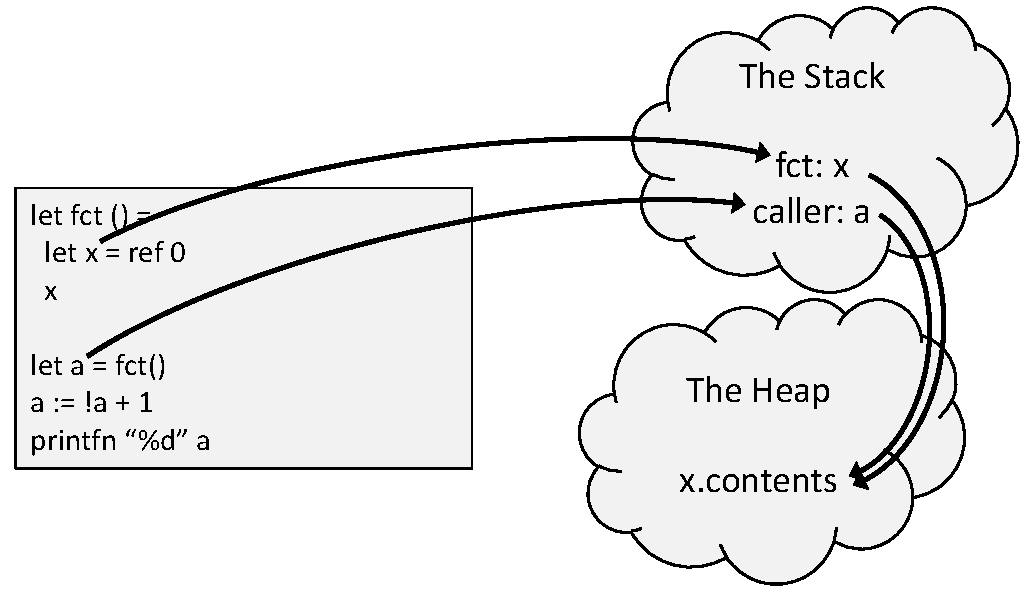
\includegraphics[width=0.6\textwidth]{ReferenceCells}
  \caption{A reference cell is a pointer to The Heap, and the content is not destroyed when its reference falls out of scope.}
  \label{fig:returningRefCells}
\end{figure}
%

Reference cells may cause \idx[side-effect]{side-effects}, where variable changes are performed across independent scopes. Some side-effects are useful, e.g., the \lstinline{printf} family changes the content of the screen, and the screen is outside the scope of the caller.  Another example of a useful side-effect is a counter shown in \Cref{refEncapsulation}.
%
\fs{refEncapsulation}{An increment function with a local state using a reference cell.}
%
Here \lstinline{incr} is an anonymous function with an internal state \lstinline{counter}. At first glance, it may be surprising that \lstinline{incr ()} does not return the value \lstinline{1} at every call. The reason is that the value of the \lstinline{incr} is the closure of the anonymous function \lstinline{fun () -> counter := ...}, which is 
\begin{equation}
  \text{\lstinline{incr}}: \left(\text{args}, \text{exp}, \text{env}\right)  = \big((), \left(\begin{subarray}{l}\displaystyle\text{\lstinline{counter := !counter + 1}}\\\displaystyle\text{\lstinline{!counter}}\end{subarray}\right), (\text{\lstinline{counter}}\rightarrow\text{\lstinline{ref 0}})\big).
\end{equation}
Thus, \lstinline{counter} is only initiated once at the initial binding, while every call of \lstinline{incr ()} updates its value on The Heap. Such a programming structure is called \idx{encapsulation}, since the \lstinline{counter} state has been encapsulated in the anonymous function, and the only way to access it is by calling the same anonymous function. In general, it is advisable to \advice{use encapsulation to hide implementation details irrelevant to the user of the code.}

The \lstinline{incr} example in \Cref{refEncapsulation} is an example of a useful side-effect. An example to be avoided is shown in \Cref{refSideEffect}.
%
\fs{refSideEffect}{Intertwining independent scopes is typically a bad idea.}
%
In the example, the function \lstinline{updateFactor} changes a variable in the scope of the function \lstinline{multiplyWithFactor}. The code style is prone to errors, since the computations are not local at the place of writing, i.e., in \lstinline{multiplyWithFactor}, and if \lstinline{updateFactor} were defined in a library, then the source code may not be available. Better style of programming is shown in \Cref{refWithoutSideEffect}.
%
\fs{refWithoutSideEffect}{A solution similar to \Cref{refSideEffect} without side-effects.}
%
Here, there can be no doubt in \lstinline{multiplyWithFactor} that the value of \lstinline{a} is changing. Side-effects do have their use, but should, in general, be avoided at almost all costs, and it is advised to \advice{minimize the use of side effects}.

Reference cells give rise to an effect called \idx{aliasing}, where two or more identifiers refer to the same data, as illustrated in \Cref{refCellAliasing}.
%
\fs{refCellAliasing}{Aliasing can cause surprising results and should be avoided.}
%
Here, \lstinline!a! is defined as a reference cell, and by defining \lstinline!b! to be equal to \lstinline!a!, we have created an alias. This can be very confusing since as the example shows, changing the value of \lstinline!b! causes \lstinline!a! to change as well. Aliasing is a variant of side-effects, and \advice{aliasing should be avoided at all costs}.

Since F\# version 4.0, the compiler has automatically converted mutable variables to reference cells, where needed.  E.g., \Cref{refEncapsulation} can be rewritten using a mutable variable, as shown in \Cref{mutableEncapsulation}.
% 
\fs{mutableEncapsulation}{Local mutable content can be indirectly accessed outside its scope.}
% 
Reference cells are preferred over mutable variables for encapsulation, in order to avoid confusion.

\section{Tuples}
\idx[tuple]{Tuples} are a direct extension of constants. They are immutable and have neither concatenations nor indexing operations. Tuples are unions of immutable types and have the following syntax:
%
\begin{verbatimwrite}{\ebnf/tuples.ebnf}
<*expr*>{*, <*expr*>*}
\end{verbatimwrite}
\syntax{\ebnf/tuples.ebnf}{Tuples are list of expressions separated by commas.}
%
Tuples are identified by the \lexeme{,} lexeme and often enclosed in parentheses, but that is not required. An example is a triple, also known as a 3-tuple, \lstinline!(2,true,"hello")!. In interactive mode, the type of tuples is demonstrated in \Cref{tuple}.
%
\fsOutput{tuple}{Tuple types are products of sets.}
%
The values \lstinline!2!, \lstinline!true!, and \lstinline!"hello"! are \idx[member]{members}, and the number of elements of a tuple is its \idx{length}. From the response of F\#, we see that the tuple is inferred to have the type \lstinline!int * bool * string!. The \lexeme{*} denotes the Cartesian product between sets.  Tuples can be products of any types and follow the lexical scope rules like value and function bindings. Notice also that a tuple may be printed as a single entity by the \lstinline!%A! %
placeholder. In the example we bound \lstinline!tp! to the tuple. The opposite is also possible, as demonstrated in \Cref{tupleDeconstruction}.
%
\fsOutput{tupleDeconstruction}{Definition of a tuple.}
%
In this example, a function is defined that takes 1 argument, a 3-tuple. If we wanted a function with 3 arguments, then the function binding should have been \lstinline{let deconstructNPrint a b c = ...}. The value binding \lstinline{let (a, b, c) = tp}, binds a tuple with 3 named members to a value, thus deconstructing it in terms of its members. This is called pattern matching and will be discussed in further details in \Cref{chap:patterns}. Since we used the \lstinline!\%A! placeholder in the \lstinline!printfn! function, the function can be called with 3-tuples of different types. F\# informs us that the tuple type is variable by writing \lstinline{'a * 'b * 'c}. The \lexeme{'} notation means that the type can be decided at run-time, see \Cref{sec:variableTypes} for more on variable types. 

Pairs or 2-tuples are so common that F\# includes two built-in functions,\idx[fst@\lstinline{fst}]{\keyword{fst}} and \idx[snd@\lstinline{snd}]{\keyword{snd}}, to extract the first and second element of a pair. This is demonstrated in \Cref{pair}.
%
\fs{pair}{Deconstruction of pairs with the built-in functions \keyword{fst} and \keyword{snd}.}
%

Tuples of equal lengths can be compared, and the  comparison is defined similarly to string comparison. Tuples of equal length are compared element by element. E.g., \lstinline!(1,2) = (1,3)! is false, while \lstinline!(1,2) = (1,2)! is true. The \lexeme{<>} operator is the boolean negation of the \lexeme{=} operator. For the \lexeme{<} , \lexeme{<=}, \lexeme{>}, and \lexeme{>=} operators, the strings are ordered lexicographically, such that \lstinline!('a', 'b', 'c') < ('a', 'b', 's') && ('a', 'b', 's') <  ('c', 'o', 's')! is true, that is, the \lexeme{<} operator on two tuples is true if and only if the left operand should come before the right when sorting alphabetically. See \Cref{tupleCompare} for an example.
%
\fs{tupleCompare}{Tuples comparison is similar to string comparison.}
%
The algorithm for deciding the boolean value of \lstinline!(a1, a2) < (b1, b2)! is as follows: we start by examining the first elements, and if \lstinline!a1! and \lstinline!b1! are different, then the result of \lstinline!(a1, a2) < (b1, b2)! is equal to the result of \lstinline!a1 < b1!. If \lstinline!a1! and \lstinline!b1! are equal, then we move on to the next letter and repeat the investigation. The \lexeme{<=}, \lexeme{>}, and \lexeme{>=} operators are defined similarly.

Binding tuples to mutables does not make the tuple mutable. This is demonstrated in \Cref{tupleOfMutables}.
%
\fs{tupleOfMutables}{A mutable changes value, but the tuple defined by it does not refer to the new value.}
%
However, it is possible to define a mutable variable of type tuple such that new tuple values can be assigned to it, as shown in \Cref{mutableTuple}.
%
\fs{mutableTuple}{A mutable tuple can be assigned a new value.}
%
Mutable tuples are value types, meaning that binding to new names makes copies, not aliases, as demonstrated in \Cref{mutableTupleValue}.
%
\fs{mutableTupleValue}{A mutable tuple is a value type.}
%
The use of tuples shortens code and highlights semantic content at a higher level, e.g., instead of focusing on the elements, tuples focus on their union. While this may look elegant and short there is the risk of \idx{obfuscation}, i.e., writing compact code that is difficult to read, where an unprepared reader of the code may not easily understand the computation nor appreciate its elegance without an accompanying explanation.  Hence, \advice{always keep an eye out for compact and concise ways to write code, but never at the expense of readability.}

%%% Local Variables:
%%% TeX-master: "fsharpNotes"
%%% End:



\chapter{Comments}
\label{chap:comments}

\jon{\url{https://msdn.microsoft.com/en-us/visualfsharpdocs/conceptual/code-formatting-guidelines-%5Bfsharp%5D}, \url{https://blogs.msdn.microsoft.com/chrsmith/2008/06/25/some-guidelines-for-readable-f-code/}, \url{http://fsharp.org/specs/component-design-guidelines/}, \url{https://github.com/dungpa/fantomas/blob/master/docs/FormattingConventions.md}}


\begin{lstlisting}
/// <summary>Make a new matrix whos result is the matrix product of this with other.</summary>
/// <param name="other">A matrix, must have same size number of rows as this has columns.</param>
/// <returns>A new matrix.</returns>
/// <exception cref="System.ArgumentException">Thrown when the number of columns in this is different that the number of rows in other.</exception>
member Mul : other:Matrix -> Matrix

\end{lstlisting}

%%% Local Variables:
%%% TeX-master: "fsharpNotes"
%%% End:


\documentclass[fsharpnotes.tex]{subfiles}
\graphicspath{ {./figures/} }

\begin{document}
\chapter{Controlling Program Flow}
\label{chap:flow}
Non-recursive functions encapsulate code and allow for control of execution flow. That is, if a piece of code needs to be executed many times, then we can encapsulate it in the body of a function and call this function several times. In this chapter, we will look at more general control of flow via loops and conditional execution. Recursion is another mechanism for controlling flow, but this is deferred to \Cref{sec:recursion}.

\section{While and For Loops}
Many programming constructs need to be repeated, and F\# contains many structures for repetition. A \idx[while@\lstinline{while}]{\keyword{while}}-loop has the following syntax:
%
\begin{verbatimwrite}{\ebnf/whileLoop.ebnf}
while <*condition*> do <*expr*> [*done*]
\end{verbatimwrite}
\syntax{\ebnf/whileLoop.ebnf}{While loop.}
%
The \idx{condition} \lstinline[language=syntax]{<*condition*>} is an expression that evaluates to true or false. A while-loop repeats the \lstinline[language=syntax]{<*expr*>} expression as long as the condition is true.  Using lightweight syntax, the block following the \idx[do@\lstinline{do}]{\keyword{do}} keyword up to and including the \idx[done@\lstinline{done}]{\keyword{done}} keyword may be replaced by a newline and indentation.

The program in \Cref{count} is an example of a while-loop which counts from 1 to 10.
%
\fs{countWhile}{Count to 10 with a counter variable.}
%
The variable \lstinline{i} is customarily called the counter variable. The counting is done by performing the following computation: In line~\ref{countWhileLoop}, the counter variable is first given an initial value of 1. Then execution enters the while-loop and examines the condition. Since $1 <= 10$, the condition is true, and execution enters the body of the loop. The body prints the value of the counter to the screen and increases the counter by 1. Then execution returns to the top of the while-loop. Now the condition is $2 <= 10$, which is also true, and so execution enters the body and so on until the counter has reached the value 11, in which case the condition $11 <= 10$ is false, and execution continues in line~\ref{countWhileContinue}.

In lightweight syntax, this would be as shown in \Cref{countWhileLightweight}.
%
\fs{countWhileLightweight}{Count to 10 with a counter variable using lightweight syntax.}
%
Notice that although the expression following the condition is preceded with a \keyword{do} keyword, and \lstinline[language=syntax]{do <*expr*>} is a \lstinline{do}-binding, the keyword \keyword{do} is mandatory. 

Counters are so common that a special syntax has been reserved for loops using counters. These are called \idx[for@\lstinline{for}]{\keyword{for}}-loops. For-loops come in several variants, and here we will focus on the one using an explicit counter. Its syntax is:
%
\begin{verbatimwrite}{\ebnf/forLoop.ebnf}
for <*ident*> = <*firstExpr*> to <*lastExpr*> do <*bodyExpr*> [*done*]
\end{verbatimwrite}
\syntax{\ebnf/forLoop.ebnf}{For loop.}
%
A for-loop initially binds the counter identifier \lstinline[language=syntax]{<*ident*>} to be the value \lstinline[language=syntax]{<*firstExpr*>}. Then execution enters the body, and \lstinline[language=syntax]{<*bodyExpr*>} is evaluated. Once done, the counter is increased, and execution evaluates \lstinline[language=syntax]{<*bodyExpr*>}  once again. This is repeated as long as the counter is not greater than \lstinline[language=syntax]{<*lastExpr*>}. As for while-loops, when using lightweight syntax the block following the \idx[do@\lstinline{do}]{\keyword{do}} keyword up to and including the \idx[done@\lstinline{done}]{\keyword{done}} keyword may be replaced by a newline and indentation.

The counting example from \Cref{countWhile} using a \keyword{for}-loop is shown in \Cref{count}
%
\fs{count}{Counting from 1 to 10 using a \keyword{for}-loop.}
%
As this interactive script demonstrates, the identifier \lstinline!i! takes all the values between 1 and 10, but in spite of its changing state, it is not mutable. Note also that the return value of the \keyword{for} expression is \lexeme{()}, like the \lstinline!printf! functions. The lightweight equivalent is shown in \Cref{countLightweight}.
%
\fs{countLightweight}{Counting from 1 to 10 using a \keyword{for}-loop using the lightweight syntax.}
%

To further compare for- and while-loops, consider the following problem.
\begin{problem}
  Write a program that calculates the $n$'th Fibonacci number.
\end{problem}
Fibonacci numbers is a sequence of numbers starting with $1, 1$, and where the next number is calculated as the sum of the previous two. Hence the first ten numbers are: $1, 1, 2, 3, 5, 8, 13, 21, 34, 55$. Fibonacci numbers are related to Golden spirals shown in \Cref{fig:goldenSpiral}.
\begin{figure}
  \centering
  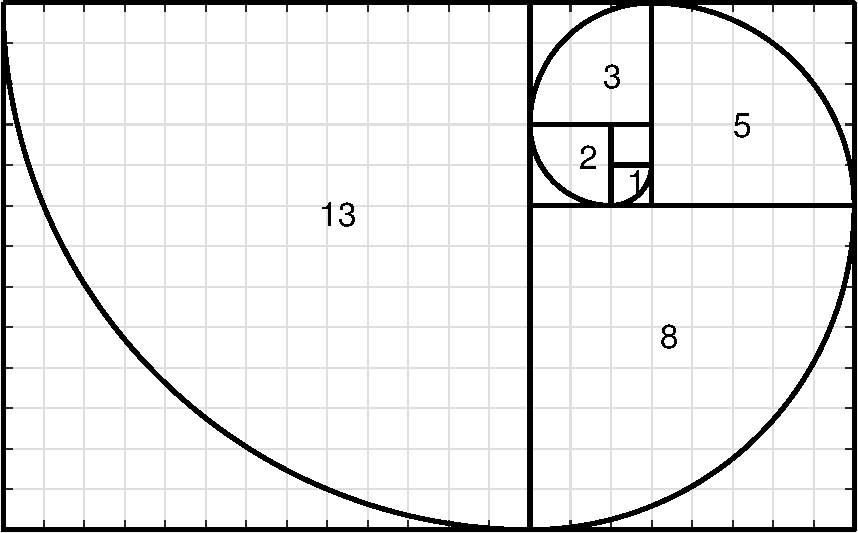
\includegraphics[width=0.45\linewidth]{Fibonacci_spiral}
  \caption{The Fibonacci spiral is an approximation of the golden spiral. Each square has side lengths of successive Fibonacci numbers, and the curve in each square is the circular arc with a radius of the square it is drawn in.}
  \label{fig:goldenSpiral}
\end{figure}
Often the sequence is extended with a preceding number $0$, to be $0, 1, 1, 2, 3, \dots$, which we will do here as well.

We could solve this problem with a \keyword{for}-loop, as shown in \Cref{fibFor}.
%
\fs{fibFor}{The $n$'th Fibonacci number calculated using a for-loop.}
%
The basic idea of the solution is that if we are given the $(n-1)$'th and $(n-2)$'th numbers, the $n$'th number is trivial to compute. And assuming that $\text{fib}(1)$ and $\text{fib}(2)$ are given, then it is trivial to calculate $\text{fib}(3)$. For $\text{fib}(4)$, we only need $\text{fib}(3)$ and $\text{fib}(2)$, hence we may disregard $\text{fib}(1)$. Thus, we realize that we can cyclicly update the previous, current, and next values by shifting values until we have reached the desired $\text{fib}(n)$. This is implement in \Cref{fibFor} as the function \lstinline{fib}, which takes an integer \lstinline{n} as argument and returns the $n$'th Fibonacci number. The function does this iteratively using a \keyword{for}-loop, where \lstinline{i} is the counter value, and \lstinline{pair} is the pair of the $i-1$'th and $i$'th Fibonacci numbers. In the body of the loop, the $i$'th and $i+1$'th numbers are assigned to \lstinline{pair}. The \keyword{for}-loop automatically updates \lstinline{i} for next iteration. When $n<2$ the body of the for-loop is not evaluated, and $1$ is returned. This is of course wrong for $n < 1$, but we will ignore this for now.

\Cref{fibWhile} shows a program similar to \Cref{fibFor} using a while-loop instead of for-loop.
%
\fs{fibWhile}{The $n$'th Fibonacci number calculated using a while-loop.}
%
The programs are almost identical. In this case, the \keyword{for}-loop is to be preferred, since more lines of code typically mean more chances of making a mistake.  However, while-loops are somewhat easier to argue correctness about.

The correctness of \lstinline!fib! in \Cref{fibWhile} can be proven using a \idx{loop invariant}. An \idx{invariant} is a statement that is always true at a particular point in a program, and a loop invariant is a statement which is true at the beginning and end of a loop. In line~\ref{fibWhileInvariant} in \Cref{fibWhile}, we may state the invariant: The variable \lstinline{pair} is the pair of the $i-1$'th and $i$'th Fibonacci numbers. This is provable by induction:
\begin{description}
\item[Base case:]  Before entering the while loop, \lstinline{i} is 1, \lstinline{pair} is (0, 1). Thus, the invariant is true.
\item[Induction step:] Assuming that \lstinline{pair} is the $i-1$'th and $i$'th Fibonacci numbers, the body first assigns a new value to \lstinline{pair} as the $i$'th and $i+1$'th Fibonacci numbers, then increases $i$ by one such that at the end of the loop the \lstinline{pair} again contains the the $i-1$'th and $i$'th Fibonacci numbers. \end{description}
Thus, since our invariant is true for the first case, and any iteration following an iteration where the invariant is true, is also true, then it is true for all iterations.

Thus we know that the second value in \lstinline{pair} holds the value of the $i$'th Fibonacci number, and since we further may prove that $i = n$ when line~\ref{fibWhileInvariantContinue} is reached, then it is proven that \lstinline{fib} returns the $n$'th Fibonacci number. 

While-loops also allow for logical structures other than for-loops, such as the case when the number of iteration cannot easily be decided when entering the loop. As an example, consider a slight variation of the above problem, where we wish to find the largest Fibonacci number less or equal some number. A solution to this problem is shown in \Cref{fibWhileLargest}.
%
\fs{fibWhileLargest}{Search for the largest Fibonacci number less than a specified number.}
%
The strategy here is to iteratively calculate Fibonacci numbers until we've found one larger than the argument \lstinline{n}, and then return the previous. This could not be calculated with a for-loop.

\section{Conditional Expressions}
Programs often contain code which should only be executed under certain conditions. This can be expressed with \keyword{if}-expressions, whose syntax is as follows.\idxs{if@\lstinline{if}}\idxs{then@\lstinline{then}}\idxs{elif@\lstinline{elif}}\idxs{else@\lstinline{else}}
%
\begin{verbatimwrite}{\ebnf/conditional.ebnf}
if <*cond*> then <*expr*> {*elif <*cond*> then <*expr*>*} [*else <*expr*>*]
\end{verbatimwrite}
\syntax{\ebnf/conditional.ebnf}{Conditional expressions.}
%
The condition \lstinline[language=syntax]{<*con*>} is an expression resulting in a Boolean value, and there can be zero or more \keyword{elif} conditions, as indicated by \lstinline[language=syntax]{{**}}. Each expression \lstinline[language=syntax]{<*expr*>}  is called a \idx{branch}, and all branches must have the same type, such that regardless of which branch is chosen, the type of the result of the conditional expression is the same. Then the expression of the first if-branch, whose condition is true, is evaluate. If all conditions are false then the \keyword{else}-branch is evaluated. If no \keyword{else} expression is present, then \lexeme{()} will be returned. See \Cref{condition} for a simple example.
%
\fs{condition}{Conditions evaluate their branches depending on the value of the condition.}
%
The lightweight syntax allows for newlines entered everywhere, but indentation must be used to express scope. 

To demonstrate conditional expressions, let us write a program which writes the sentence ``I have n apple(s)'', where the plural 's' is added appropriately for various $n$'s. This is done in \Cref{conditionalLightweight}, using the lightweight syntax.
%
\fs{conditionalLightweight}{Using conditional expression to generate different strings.}
%
The sentence structure and its variants give rise to a more compact solution, since the language to be returned to the user is a variant of "I have/owe no/number apple(s)", i.e., certain conditions determine whether the sentence should use ``have'' and ``owe'' and so forth. So, we could instead make decisions on each of these sentence parts, and then built the final sentence from its parts. This is accomplished in the following example:
%
\fs{conditionalLightweightAlt}{Using sentence parts to construct the final sentence.}
%
While arguably shorter, this solution is also denser, and most likely more difficult to debug and maintain.

Note that both \keyword{elif} and \keyword{else} branches are optional, which may cause problems. For example, both
\begin{quote}
\mbox{\lstinline!let a = if true then 3!}
\end{quote}
and
\begin{quote}
\mbox{\lstinline!let a = if true then 3 elif false then 4!}
\end{quote}
are invalid, since F\# is not smart enough to realize that the type of the expression is uniquely determined. Instead, F\# looks for the \keyword{else} to ensure all cases have been covered, and that \lstinline!a! always will be given a unique value of the same type regardless of the branch taken in the conditional statement. Hence,
\begin{quote}
\mbox{\lstinline!let a = if true then 3 else 4!}
\end{quote}
is the only valid expression of the 3. In practice, F\# assumes that the omitted branch returns \lexeme{()}, and thus it is fine to say \mbox{\lstinline!let a = if true then ()!} and \mbox{\lstinline!if true then printfn "hej"!}. Nevertheless, it is good practice in F\# to always include an \keyword{else} branch.
\clearpage

\section{Programming Intermezzo: Automatic Conversion of Decimal to Binary Numbers}
Using loops and conditional expressions, we are now able to solve the following problem:
\begin{problem}
  Given an integer on decimal form, write its equivalent value on the binary form.
\end{problem}
To solve this problem, consider odd numbers: They all have the property that the least significant bit is 1, e.g., $1_2 = 1, 101_2 = 5$, in contrast to even numbers such as $110_2 = 6$. Division by 2 is equal to right-shifting by 1, e.g., $1_2/2 = 0.1_2 = 0.5, 101_2/2 = 10.1_2 = 2.5, 110_2/2 = 11_2 = 3$. Thus, through dividing by 2 and checking the remainder, we may sequentially read off the least significant bit. This leads to the algorithm shown in \Cref{dec2bin}.
%
\fs{dec2bin}{Using integer division and remainder to write any positive integer in binary form.}
%
In the code, the states \lstinline!v! and \lstinline!str! are iteratively updated until \lstinline!str! finally contains the desired solution.

To prove that \Cref{dec2bin} calculates the correct sequence, we use induction. First we realize that for $v < 1$, the while-loop is skipped, and the result is trivially true. We will concentrate on line~\ref{dec2binWhile} in \Cref{dec2bin} and will prove the following loop invariant: The string \lstinline{str} contains all the bits of \lstinline{n} to the right of the bit pattern remaining in variable \lstinline{v}.
\begin{description}
\item[Base case $n=000\ldots000x$:] If $n$ only uses the lowest bit, then $n=0$ or $n=1$. If $n=0$, then it is trivially correct. Considering the case $n=1$: Before entering into the loop, \lstinline{v} is 1, and \lstinline{str} is the empty string, so the invariant is true. The condition of the while-loop is $1>0$, so execution enters the loop. Since integer division of 1 by 2 gives 0 with remainder 1, \lstinline{str} is set to \lstinline{"1"} and \lstinline{v} to 0. Now we reexamine the while-loop's condition, $0>0$, which is false, so we exit the loop. At this point, \lstinline{v} is 0 and \lstinline{str} is \lstinline{"1"}, so all bits have been shifted from \lstinline{n} to \lstinline{str}, and none are left in \lstinline{v}. Thus the invariant is true. Finally, the program returns \lstinline{"0b1"}.
\item[Induction step:] Consider the case of $n>1$, and assume that the invariant is true when entering the loop, i.e., that $m$ bits already have been shifted to \lstinline{str} and that $n>2^m$. In this case, \lstinline{v} contains the remaining bits of \lstinline{n}, which is the integer division \lstinline{v = n / 2**m}. Since $n>2^m$, \lstinline{v} is non-zero, and the loop conditions is true, so we enter the loop body. In the loop body we concatenate the rightmost bit of \lstinline{v} to the left of \lstinline{str} using \lstinline{v % 2}, %
and right-shift \lstinline{v} one bit to the right with \lstinline{v <- v / 2}. Thus, when returning to the condition the invariant is true, since the right-most bit in \lstinline{v} has been shifted to \lstinline{str}. This continues until all bits have been shifted to \lstinline{str} and \lstinline{v = 0}, in which case the loop terminates, and \lstinline{"0b"+str} is returned.
\end{description}
Thus we have proven that \lstinline{dec2bin} correctly converts integers to strings representing binary numbers.
\end{document}



\chapter{Ordered series of data}
\label{chap:lists}\jon{possibly add maps and sets as well.}
F\# is tuned to work with ordered series, and there are several built-in lists with various properties making them useful for different tasks. E.g.,
%
\fs{tuplesQuadraticEq}{Using tuples to gather values.}
%
F\# has 4 built-in list types: strings, tuples, lists, arrays, and sequences. Strings were discussed in Chapter~\ref{chap:calculator}, and tuples, lists, arrays, and sequences following this (simplified) syntax:
%
\begin{lstlisting}[language=ebnf]
tupleList = expr | expr "," tupleList
listOrArrayList =  expr | expr ";" listOrArrayList
range-exp = expr ".." expr [".." expr]
comp-expr =
  "let" pat "=" expr "in" comp-expr
  | "use" pat = expr "in" comp-expr
  | ("yield" | "yield!") expr
  | "if" expr "then" comp-expr ["else" comp-expr]
  | "match" expr "with" comp-rules
  | "try" comp-expr "with" comp-rules
  | "try" comp-expr "finally" expr
  | "while" expr "do" expr ["done"]
  | "for" ident "=" expr "to" expr "do" comp-expr ["done"]
  | "for" pat "in" expr-or-range-expr "do" comp-expr ["done"]
  | comp-expr ";" comp-expr
short-comp-expr = "for" pat "in" (expr | range-expr) "->" expr
comp-or-range-expr = comp-expr| short-comp-expr | range-expr
comp-rule = pat pattern-guardopt "->" comp-expr
comp-rules = comp-rule | comp-rule '|' comp-rules
expr = ... 
  | tupleList
  | "[" (listOrArrayList | comp-or-range-expr) "]" (* computation list expression *)
  | "[|" (listOrArrayList | comp-or-range-expr) "|]" (* computation array expression *)
  | "seq" "{" comp-or-range-expr "}" (* computation expression *)
  | ...
\end{lstlisting}
%
\jon{Spec-4.0: grammar for list and array expressions are subsets of computation list and array expressions.}\jon{pat is not explained, see Spec-4.0 Chapter 7.}Tuples are a direct extension of constants. They are immutable and do not have concatenations nor indexing operations. This is in contrast to lists. Lists are also immutable, but have a simple syntax for concatenation and indexing. Arrays are mutable lists, and support higher order structures such as tables and 3 dimensional arrays. Sequences are like lists, but with the added advantage of a very flexible construction mechanism, and the option of representing infinite long sequences. In the following, we will present these data structures in detail.

\section{Tuples}
\idx[tuple]{Tuples} are unions of immutable types, 
%
\begin{lstlisting}[language=ebnf]
tupleList = expr | expr "," tupleList
expr = ... 
  | tupleList
  | ...
\end{lstlisting}
%
and the they are identified by the \lexeme{,} lexeme. Most often the tuple is enclosed in parentheses, but that is not required. Consider the tripel, also known as a 3-tuple, \lstinline!(2,true,"hello")! in interactive mode,
%
\fso{tuple}{Definition of a tuple.}
%
The values \lstinline!2!, \lstinline!true!, and \lstinline!"hello"! are \idx[member]{members}, and the number of elements of a tuple is its \idx{length}. From the response of F\# we see that the tuple is inferred to have the type \lstinline!int * bool * string!, where the \lexeme{*} is cartesian product between the three sets.  Notice, that tuples can be products of any types and have lexical scope like value and function bindings. Notice also, that a tuple may be printed as a single entity by the \lstinline!%A! placeholder. In the example, we bound \lstinline!tp! to the tuple, the opposite is also possible,
%
\fso{tupleDeconstruction}{Definition of a tuple.}
%
In this a function is defined that takes 1 argument, a 3-tuple, and which is bound to a tuple with 3 named members. Since we used the \lstinline!%A! placeholder in the \lstinline!printfn! function, then the function is generic and can be called with 3-tuples of different types. Note, \advice{don't confuse a function of $n$ arguments with a function of an $n$-tuple.}  The later has only 1 argument, and the difference is the \lexeme{,}'s. Another example is \lstinline!let solution a b c = ...!, which is the beginning of the function definition in Listing~\ref{tuplesQuadraticEq}. It is a function of 3 arguments, while \lstinline!let solution (a, b, c) = ...! would be a function of 1 argument, which is a 3-tuple. Functions of several arguments makes currying easy, i.e., we could define a new function which fixes the quadratic term to be 0 as \lstinline!let solutionToLinear = solution 0.0!, that is, without needing to specify anything else. With tuples, we would need the slightly more complicated, \lstinline!let solutionToLinear (b, c) = solution (0.0, b, c)!.

Tuples comparison are defined similarly as strings. Tuples of different lengths are different. For tuples of equal length, then they are compared element by element. E.g., \lstinline!(1,2) = (1,3)! is false, while \lstinline!(1,2) = (1,2)! is true. The \lexeme{<>} operator is the boolean negation of the \lexeme{=} operator. For the \lexeme{<} , \lexeme{<=}, \lexeme{>}, and \lexeme{>=} operators, the strings are ordered alphabetically like, such that \lstinline!('a', 'b', 'c') < ('a', 'b', 's') && ('a', 'b', 's') <  ('c', 'o', 's')! is true, that is, the \lexeme{<} operator on two tuples is true, if the left operand should come before the right, when sorting alphabetically like. 
%
\fs{tupleCompare}{Tuples are compared as strings are compared alphabetically.}
%
The algorithm for deciding the boolean value of \lstinline!(a1, a2) < (b1, b2)! is as follows: we start by examining the first elements, and if \lstinline!la1! and \lstinline!b1! are different, then the \lstinline!(a1, a2) < (b1, b2)! is equal to \lstinline!a1 < b1!. If \lstinline!la1! and \lstinline!b1! are equal, then we move onto the next letter and repeat the investigation. The \lexeme{<=}, \lexeme{>}, and \lexeme{>=} operators are defined similarly.

Binding tuples to mutuals does not make the tuple mutable, e.g.,
%
\fs{tupleOfMutables}{A mutable change value, but the tuple defined by it does not refer to the new value.}
%
However, tuples may be mutual such that new tuple values can be assigned to it, e.g., in the Fibonacci example, we can write a more compact script by using mutable tuples and the \keyword{fst} and \keyword{snd} functions as follows.
%
\fs{fibTuple}{Calculating Fibonacci numbers using mutable tuple.}
%
In this example, the central computation has been packed into a single line, \lstinline!prev <- (snd prev, (fst prev) + (snd prev))!, where both the calculation of $\text{fib}(n) = \text{fib}(n-2) + \text{fib}(n-1)$ and the rearrangement of memory to hold the new values $\text{fib}(n)$ and $\text{fib}(n-1)$ based on the old values $\text{fib}(n-2) + \text{fib}(n-1)$. While this may look elegant and short there is the risk of \idx{obfuscation}, i.e., writing compact code that is difficult to read, and in this case, an unprepared reader of the code may not easily understand the computation nor appreciate its elegance without an accompanying explanation.  Hence, \advice{always keep an eye out for compact and concise ways to write code, but never at the expense of readability.}

\section{Lists}
\idx[list]{Lists} are unions of immutable values of the same type and have a more flexible structure than tuples. Its grammar follows \idx{computation expressions}, which is very rich and shared with arrays and sequences, and we will delay a discussion on most computation expressions to Section~\ref{sec:sequences}, and here just consider a subset of the grammar:
\begin{lstlisting}[language=ebnf]
listOrArrayList =  expr | expr ";" listOrArrayList
range-exp = expr ".." expr [".." expr]
expr = ... 
  | "[" (listOrArrayList | ... | range-expr) "]" (* computation list expression *)
  | ...
\end{lstlisting}
Simple examples of a list grammars are, \lstinline[language=ebnf]![expr; expr; ... ; expr]!, \lstinline[language=ebnf]![expr ".." expr]!, \lstinline[language=ebnf]![expr ".." expr ".." expr]!, e.g., an explicit list \lstinline!let lst = [1; 2; 3; 4; 5]!, which may be written shortly as \idx{range expression} as \lstinline!let lst = [1 .. 5]!, and ranges may include a step size \lstinline!let lst = [1 .. 2 .. 5]!, which is the same as \lstinline!let lst = [1; 3; 5]!.

Lists may be indexed and concatenated much like strings, e.g.,
%
\fs{listIndexing}{Examples of list concatenation, indexing.}
%
A list type is identified with the \keyword{list} keyword, as here a list of integers is \lstinline!int list!. Above, we used the \idx{\lexeme{@}} and \idx{\lexeme{::}} concatenation operators, the \idx{\lexeme{.[]}} index method, and the \idx{\lexeme{Length}} property. Notice, as strings, list elements are counted from 0, and thus the last element has \lstinline!lst.Length - 1!. In \lstinline!printList! the \keyword{for}-\keyword{in} is used, which runs loops through each element of the list and assigns it to the identifier \lstinline!elm!. This is in contrast to \lstinline!printListAlt!, which uses uses the \keyword{for}-\keyword{to} keyword and explicitly represents the index \lstinline!i!. Explicit representation of the index makes more complicated programs, and thus increases the chances of programming errors. Hence, \advice{\keyword{for}-\keyword{in} is to be preferred over \keyword{for}-\keyword{to}.} Lists support slicing identically to strings, e.g.,
%
\fs{listSlicing}{Examples of list slicing. Compare with Listing~\ref{stringIndexing}.}
%

Lists are well suited for recursive functions and pattern matching with, e.g., \keyword{match}-\keyword{with} as illustrated in the next example:
%
\fs{listPatternMatching}{Examples of list concatenation, indexing.}
%
The pattern \lstinline!l::rest! is the pattern for the first element followed by a list of the rest of the list. This pattern matches all lists except an empty list, hence \lstinline!rest! may be empty. Thus the wildcard pattern matching anything including the empty list, will be used only when \lstinline!lst! is empty.

\idx[pattern matching]{Pattern matching} with lists is quite powerful, consider the following problem:
\begin{problem}
  Given a list of pairs of course names and course grades, calculate the average grade.
\end{problem}
A list of course names and grades is \lstinline![("name1", grade1); ("name2", grade2); ...]!. Let's take a recursive solution. First problem will be to iterate through the list. For this we can use pattern matching similarly to Listing~\ref{listPatternMatching} with \lstinline!(name, grade)::rest!. The second problem will be to calculate the average. The average grade is the sum all grades and divide by the number of grades. Assume that we already have made a function, which calculates the \lstinline!sum! and \lstinline!n!, the sum and number of elements, for \lstinline!rest!, then all we need is to add \lstinline!grade! to the \lstinline!sum! and \lstinline!1! to \lstinline!n!. For an empty list, \lstinline!sum! and \lstinline!n! should be \lstinline!0!. Thus we arrive at the following solution,
% However, an elegant alternative is available as
% \fs{flowForLists}{}
% This to be preferred, since we completely can ignore list boundary conditions and hence avoid out of range indexing. For comparison see a recursive implementation of the same,
%
\fs{avgGradesRec}{Calculating a list of average grades using recursion and pattern matching.}
%
%Note how this implementation avoids the use of variables in contrast to the previous examples.

Pattern matching and appending is a useful combination, if we wish to produce new from old lists. E.g., a function returning a list of squared entries of its argument can be programmed as,
%
\fs{listSquare}{Using pattern matching and list appending elements to lists.}
%
This is a prototypical functional programming style solution, and which uses the \lexeme{::} for 2 different purposes: First the list \lstinline![1 .. 10]! is first matched with \lstinline!1 :: [2 .. 10]!, and then we assume that we have solved the problem for \lstinline!square rest!, such that all we need to do is append \lstinline!1*1! to the beginning output from \lstinline!square rest!. Hence we get, \lstinline!square [1 .. 10]! $\curvearrowright$ \lstinline!1 * 1 :: square [2 .. 10]! $\curvearrowright$ \lstinline!1 * 1 :: (2 * 2 :: square [3 .. 10])! $\curvearrowright$ \dots \lstinline!1 * 1 :: (2 * 2 :: ... 10 * 10 :: [])!, where the stopping criterium is reached, when the \lstinline!elm :: rest! does not match with a, hence it is empty, which does match the wildcard pattern \lexeme{_}. More on functional programming in Section~\ref{chap:functional}

The basic properties and members of lists are summarized in Table~\ref{tab:list}.\idxss{Length}\idxss{List.Empty}\idxss{IsEmpty}\idxss{Item}\idxss{Head}\idxss{Tail}\idxss{Cons}
\begin{table}
  \centering
  \begin{tabularx}{\linewidth}{|>{\hsize=.5\hsize}X|>{\hsize=1.5\hsize}X|>{\hsize=1\hsize}X|}
    \hline
    Function name & Example & Description\\
    \hline
    \lstinline!Length! & \fsi{listLength}{1.5} & The number of elements in a list\\
    \hline
    \lstinline!List.Empty! & \fsi{listEmpty}{1.5} & An empty list of specified type\\
    \hline
    \lstinline!IsEmpty! & \fsi{listIsEmpty}{1.5} & Compare with the empty list\\
    \hline
    \lstinline!Item! & \fsi{listItem}{1.5} & Indexing\\
    \hline
    \lstinline!Head! & \fsi{listHead}{1.5} & The first element in the list. Exception if empty.\\
    \hline
    \lstinline!Tail! & \fsi{listTail}{1.5} & The list except its first element. Exception if empty.\\
    \hline
    \lstinline!Cons! & \fsi{listCons}{1.5} & Append an element to the front of the list\\
    \hline
    \lstinline!@! & \fsi{listConcatenate}{1.5} & Concatenate two lists\\
    \hline
  \end{tabularx}
  \caption{Basic properties and members of lists. The syntax used in \lstinline{List<int>.Empty} ensures that the empty list is of type \lstinline{int}.}
  \label{tab:list}
\end{table}
In addition, lists have many other built-in functions, such as functions for converting lists to arrays and sequences,\idxss{List.toList}\idxss{List.toArray}
%
\fs{listConversion}{The \lstinline!List! module contains functions for conversion to arrays and sequences.}
%
These and more will be discussed in Chapter~\ref{chap:collection} and Part~\ref{part:declarative}.

It is possible to make multidimensional lists as lists of lists, e.g., 
%
\fs{listMultidimensional}{A ragged multidimensional list, built as lists of lists, and its indexing.}
%
The example shows a \idx{ragged multidimensional list}, since each row has different number of elements. The indexing of a particular element is not elegant, which is why arrays are often preferred in F\#.

\section{Arrays}
\label{sec:arrays}
%\subsection{1 dimensional arrays}
One dimensional arrays or just arrays for short are mutable lists of the same type and follow a similar syntax as lists. Its grammar follows \idx{computation expressions}, which will be discussed in Section~\ref{sec:sequences}. Here we consider a subset of the grammar:
%
\begin{lstlisting}[language=ebnf]
listOrArrayList =  expr | expr ";" listOrArrayList
range-exp = expr ".." expr [".." expr]
expr = ... 
  | "[|" (listOrArrayList | ... | range-expr) "|]" (* computation array expression *)
  | ...
\end{lstlisting}
%
Thus the creation of arrays is identical to lists, but there is no explicit operator support for appending and concatenation, e.g.,
%
\fs{arrayCreation}{Creating arrays with a syntax similarly to lists.}
%
The array type is defined using the \keyword{array} keyword or alternatively the \keyword{[]} lexeme. Arrays cannot be resized, but are mutable,
%
\fs{arrayReassign}{Arrays are mutable in spite the missing \keyword{mutable} keyword.}
%
Notice that in spite the missing \keyword{mutable} keyword, the function \lstinline{square} still had the \idx{side-effect} of squaring alle entries in \lstinline{A}.  Arrays only support direct pattern matching, e.g.,
%
\fs{arrayPatternMatching}{Only simple pattern matching is allowed for arrays.}
%
The given example is the first example of a 2-dimensional array, which can be implemented as arrays of arrays and here written as \lstinline!string array array!. Below further discussion of on 2 and higher dimensional arrays be discussed.  Arrays support \idx{slicing}, that is, indexing an array with a range results in a copy of array with values corresponding to the range, e.g.,
%
\fs{arraySlicing}{Examples of array slicing. Compare with Listing~\ref{listSlicing} and Listing~\ref{stringIndexing}.}
%
As illustrated, the missing start or end index implies from the first or to the last element.

Arrays can be converted to lists and sequences by,\idxss{Array.toList}\idxss{Array.toArray}
%
\fs{arrayConversion}{The \lstinline!Array! module contains functions for conversion to lists and sequences.}
%
There are quite a number of built-in procedures for all arrays many which will be discussed in Chapter~\ref{chap:collection}.

%\subsection{Multidimensional Arrays}
Higher dimensional arrays can be created as arrays of arrays (of arrays \dots). These are known as \idx{jagged arrays}, since there is no inherent control of that all sub-arrays are of similar size. E.g., the following is a jagged array of increasing width,
%
\fs{arrayJagged}{An array of arrays. When row lengths are of non-equal elements, then it is a Jagged array.}
%
Indexing arrays of arrays is done sequentially, in the sense that in the above example, the number of outer arrays is \lstinline|a.Length|,  \lstinline|a.[i]| is the i'th array, the length of the i'th array is \lstinline|a.[i].Length|, and the j'th element of the i'th array is thus \lstinline|a.[i].[j]|. Often 2 dimensional rectangular arrays are used, which can be implemented as a jagged array as,
%
\fs{arrayJaggedSquare}{A rectangular array.} 
%
Notice, the \keyword{for}-\keyword{in} cannot be used in \lstinline!pownArray!, e.g., \lstinline!for row in arr do for elm in row do elm <- pown elm p done done} since the iterator value \lstinline!elm! is not mutable even though \lstinline!arr! is an array.
%
In fact, square arrays of dimensions 2 to 4 are so common that F\# has built-in modules for their support. In the following describe Array2D. The workings of Array3D and Array4D are very similar. An example of creating the same 2 dimensional array as above but as an \texttt{Array2D} is,
%
\fs{array2D}{Creating a 3 by 4 rectangular arrays of intigers.}
%
Notice that the indexing uses a slightly different notation '\verb|[,]|' and the length functions are also slightly different. The statement \verb|A.Length| would return the total number of elements in the array, in this case 12. As can be seen, the \lstinline!printf! supports direct printing of the 2 dimensional array. Higher dimensional arrays support slicing, e.g.,
%
\fs{array2DSlicing}{Examples of Array2D slicing. Compare with Listing~\ref{array2D}.}
%
Note that in almost all cases, slicing produces a sub rectangular 2 dimensional array except for \lstinline{arr.[1,*]}, which is an array, as can be seen by the single \lexeme{[}. In contrast, \lstinline{A.[1..1,*]} is an Array2D. Note also, that \lstinline!printfn! typesets 2 dimensional arrays as \lstinline{[[ ... ]]} and not \lstinline{[|[| ... |]|]}, which can cause confusion with lists of lists.
\jon{Array2D.ToString produces \lstinline{[[ ... ]]} and not \lstinline{[|[| ... |]|]}, which can cause confusion.}

Array2D and higher have a number of built-in functions that will be discussed in Chapter~\ref{chap:collection}.

\section{Sequences}
\label{sec:sequences}
Sequences are lists, where the elements are build as needed. Examples are\jon{Mono does not support specification Spec-4.0 Section 6.3.11, seq {comp-expr}, in the form seq {3} or seq {3; 4}.}
%
\fso{seqExample}{Creating sequences by range explicitly stating elements, a range expressions, a computation expression, and an infinite computation expression}
%
Sequences are built using the following subset of the general syntax,
\begin{lstlisting}[language=ebnf]
range-exp = expr ".." expr [".." expr]
comp-expr =
  "let" pat "=" expr "in" comp-expr
  | "use" pat = expr "in" comp-expr
  | ("yield" | "yield!") expr
  | "if" expr "then" comp-expr ["else" comp-expr]
  | "match" expr "with" comp-rules
  | "try" comp-expr "with" comp-rules
  | "try" comp-expr "finally" expr
  | "while" expr "do" expr ["done"]
  | "for" ident "=" expr "to" expr "do" comp-expr ["done"]
  | "for" pat "in" expr-or-range-expr "do" comp-expr ["done"]
  | comp-expr ";" comp-expr
short-comp-expr = "for" pat "in" (expr | range-expr) "->" expr
comp-or-range-expr = comp-expr| short-comp-expr | range-expr
comp-rule = pat pattern-guardopt "->" comp-expr
comp-rules = comp-rule | comp-rule '|' comp-rules
expr = ... 
  | "seq" "{" comp-or-range-expr "}" (* computation expression *)
  | ...
\end{lstlisting}
%
Sequence may be defined using simple range expressions but most often are defined as a small program, that generates values with the \keyword{yield} keyword or \keyword{yield!} keyword. The \keyword{yield!} is called \idx{yield bang}, and appends a sequence instead of adding a sequence as an element. Thus, \lstinline!seq {3; 5}! is not permitted, but \lstinline!seq {yield 3; yield 5}! and \lstinline|seq {yield! (seq {yield 3; yield 5})}| are, both creating \lstinline!seq<int> = seq [3; 5]!, i.e., a sequence of integers. Most often computation expressions are used to produced members that are not just ranges, but more complicated expressions of ranges, e.g., \lstinline!c! in the example. Sequences may even in principle be infinitely long, e.g., \lstinline!d!. Calculating the complete sequence at the point of definition is impossible due to lack of memory, as is accessing all its elements due to lack of time. But infinite sequences are still very useful, e.g., identifier \lstinline!d! illustrates the parametrization of a circle, which is an infinite domain, and any index will be converted to the equivalent 60th degree angle in radians. F\# warns against recursive values, as defined in the example, since it will check the soundness of the value at run-time rather than at compile-time. The warning can be removed by adding \lstinline!#nowarn "40"! in the script or \lstinline!--nowarn:40! as argument to \lstinline[language=console]!fsharpi! or \lstinline[language=console]!fsharpc!.

Sequences are generalisations of lists and arrays, and functions taking sequences as argument may equally take lists and arrays as argument. Sequences do not have many built-in operators, but a rich collection of functions in the \lstinline!Collections.Seq!. E.g.,\idxss{Seq.item}\idxss{Seq.take}
%
\fso{seqIndexing}{Index a sequence with \lstinline!Seq.item! and \lstinline!Seq.take!}
%
which as usual index from 0 and will cast an exception, if indexing is out of range for the sequence. 

That sequences really are programs rather than values can be seen by the following example,
%
\fso{seqDelayedEval}{Sequences elements are first evaluated, when needed.}
%
In the example, we see that the \lstinline!printfn! function embedded in the definition is first executed, when the 3rd item is requested.

\jon{Mono, missing support for Spec-4.0 Chapter 6, \lstinline!do!-\lstinline!in! in sequences. E.g., \lstinline!seq {let _ = printfn "hej" in yield 3}! is ok, but \lstinline!seq {do printfn "hej" in yield 3}! not. One could argue, that computation expression is the framework and that it is the seq implementation, which does not provide full access to the framework. but this is confusing, since seq gets special attention in the specification.}

The only difference between computation expression's programming constructs and the similar regular expressions constructs is that they must return a value with the \keyword{yield} or \keyword{yield!} keywords.\jon{Mono implements if-elif-else, but this is not in the specification.} The \keyword{try}-keyword constructions will be discussed in Chapter~\ref{chap:exceptions}, and the \keyword{use}-keyword is a variant of \keyword{let} but used in asynchronous computations, which will not be treated here.

  % "let" pat "=" expr "in" comp-expr
  % | "use" pat = expr "in" comp-expr
  % | ("yield" | "yield!") expr
  % | "if" expr "then" comp-expr ["else" comp-expr]
  % | "match" expr "with" comp-rules
  % | "try" comp-expr "with" comp-rules
  % | "try" comp-expr "finally" expr
  % | "while" expr "do" expr ["done"]
  % | "for" ident "=" expr "to" expr "do" comp-expr ["done"]
  % | "for" pat "in" expr-or-range-expr "do" comp-expr ["done"]
  % | comp-expr ";" comp-expr

Infinite sequences is a useful concept in many programs and may be generated in a number of ways. E.g., to generate a repeated sequence, we could use recursive value definition, a computation expression, a recursive function, or the \lstinline!Seq! module. Using a recursive value definition,
%
\fs{seqInfinteValue2}{Recursive value definitions gives a warning.  Compare with Listing\ref{seqInfinteValue}, \ref{seqInfinteFunction}, and \ref{seqInitInfinite}.}
%
F\# warns against using recursive values, since it will check the soundness of the value at run-time rather than at compile-time. The warning can be removed by adding \lstinline!#nowarn "40"! in the script or \lstinline!--nowarn:40! as argument to \lstinline[language=console]!fsharpi! or \lstinline[language=console]!fsharpc!, but \advice{warnings are messages from the designers of F\# that your program is non-optimal, and you should avoid structures that throw warnings instead of relying on \lstinline{\#nowarn} and similar constructions.} Instead we may create an infinite loop using the \keyword{while}-\keyword{do} computation expression, as
%
\fs{seqInfinteValue}{Infinite value definition without recursion nor warning.  Compare with Listing~\ref{seqInfinteValue2}, \ref{seqInfinteFunction}, and\ref{seqInitInfinite}.}
%
or alternatively define a recursive function,
%
\fs{seqInfinteFunction}{Recursive function definitions gives no a warning.  Compare with Listing~\ref{seqInfinteValue2}, \ref{seqInfinteValue}, and \ref{seqInitInfinite}.}
%
Infinite expressions have built-in support through the \lstinline!Seq! module using \idxss{Seq.initInfinite},
%
\fs{seqInitInfinite}{Using \lstinline{Seq.initInfinte} and a function to generate an infinte sequence. Compare with Listing~\ref{seqInfinteValue2}, \ref{seqInfinteValue}, and \ref{seqInfinteFunction}.}
%
which takes a function as argument. Here we have used currying, i.e., \lstinline!get items! is a function that takes on variable and returns a value. The use of the remainder operator makes the example rather contrived, since it might have been simpler to use the \lstinline!get! indexing function directly.

Sequences are easily converted to and from lists and arrays as,\idxss{Seq.toList}\idxss{Seq.toArray}
%
\fs{seqConversion}{Conversion between sequences and lists and arrays using the \lstinline!List! module.}
%
There are quite a number of built-in functions for sequences many which will be discussed in Chapter~\ref{chap:collection}.
 
Lists and arrays may be created from sequences through the short-hand notation called \idx[list sequence expression]{list and array sequence expressions}\idxss{array sequence expressions},
\begin{lstlisting}[language=ebnf]
expr = ... 
  | "[" (... | comp-expr | short-comp-expr | ...) "]" (* list sequence expression *)
  | "[|" (.. | comp-expr | short-comp-expr | ...) "|]" (* array sequence expression *)
  | ...
\end{lstlisting}
which implicitly creates the corresponding expression and return the result as a list or array.

% *****

% \fs{arrayJaggedCompExpr}{}
% Indexing arrays of arrays is done sequentially, in the sense that in the above example, the number of outer arrays is \verb|a.Length|,  \verb|a.[i]| is the i'th array, the length of the i'th array is \verb|a.[i].Length|, and the j'th element of the i'th array is thus \verb|a.[i].[j]|. Often 2 dimensional square arrays are used, which can be implemented as a jagged array as,
% \fs{arrayJaggedSquareCompExpr}{}
% In fact, square arrays of dimensions 2 to 4 are so common that F\# has built-in modules for their support. In the following describe Array2D. The workings of Array3D and Array4D are very similar. An example of creating the same 2 dimensional array as above but as an \texttt{Array2D} is,
% \fs{array2DCompExpr}{}
% Notice that the indexing uses a slightly different notation '\verb|[,]|' and the length functions are also slightly different. The statement \verb|A.Length| would return the total number of elements in the array, in this case 12.



%%% Local Variables:
%%% TeX-master: "fsharpNotes"
%%% End:


\chapter{Testing programs}

A software bug is an error in a computer program that causes it to produce an incorrect result or behave in an unintended manner. The term bug was used by Thomas Edison in 1878\footnote{\url{https://en.wikipedia.org/wiki/Software_bug}, possibly \url{http://edison.rutgers.edu/NamesSearch/DocImage.php3?DocId=LB003487}}, but made popular in computer science by Grace Hopper, who found a moth interferring with the electronic circuits of the Harward Mark II electromechanical computer and coined the term \idx{bug} for errors in computer programs. The original bug is shown in Figure~\ref{fig:bug}.
\begin{figure}
  \centering
  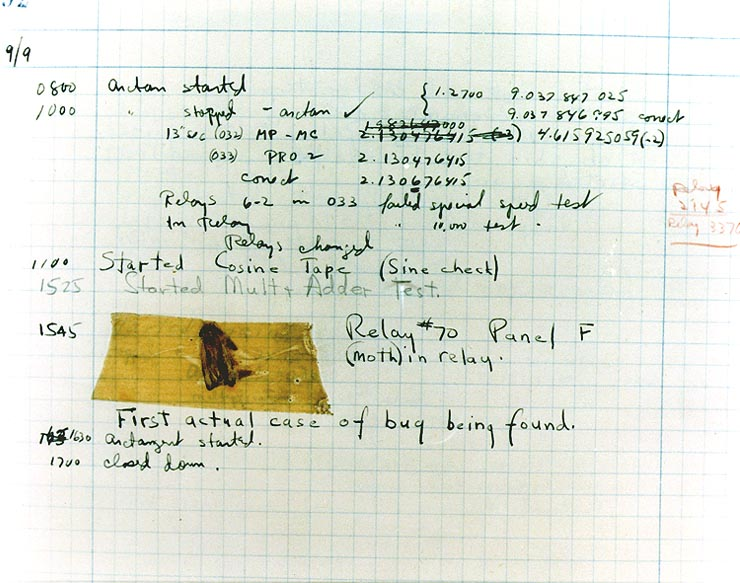
\includegraphics[width=0.45\linewidth]{H96566k}
  \caption{The first computer bug caught by Grace Hopper, U.S. Naval Historical Center Online Library Photograph NH 96566-KN.}
  \label{fig:bug}
\end{figure}
Software is everywhere, and errors therein have huge economic impact on our society and can threaten lives\footnote{\url{https://en.wikipedia.org/wiki/List_of_software_bugs}}.

The ISO/IEC organizations have developed standards for software testing\footnote{ISO/IEC 9126, International standard for the evaluation of software quality, December 19, 1991, later replaced by ISO/IEC 25010:2011}.  To illustrate basic concepts of software quality consider a hypothetical route planning system. Essential factors of its quality is,
\begin{description}
\item[Functionality:]\idxs{functionality} Does the software compile and run without internal errors. Does it solve the problem, it was intended to solve? E.g., does the route planning software finde a suitable route from point a to b?
\item[Reliability:]\idxs{reliability} Does the software work reliably over time? E.g., does the route planning software work in case of internet dropouts?
\item[Usability:]\idxs{usability} Is the software easy and intuitive to use by humans? E.g., is it easy to enter adresses and alternative routes in the software's interface?
\item[Efficiency:]\idxs{efficiency} How many computer and human resources does the software require? E.g., does it take milliseconds or hours to find a requested route? Can the software run on a mobile platform with limited computer speed and memory?
\item[Maintainability:]\idxs{maintainability} In case of the discovery of new bugs, is it easy to test and correct the software? Is it easy to extend the software with new functionality? E.g., is it easy to update the map with updated roadmaps and new information? Can the system be improved to work both for car drivers and bicyclists? 
\item[Portability:]\idxs{portability} Is it easy to port the software to new systems such as new server architecture and screen sizes? E.g., if the routing software originally was written for IOS devices, will it be easy to port to Android systems?
\end{description}
The above mentioned concepts are ordered based on the requirements of the system. Functionality and reliability ares perhaps the most important concepts, since if the software does not solve the specified problem, then the software designing process has failed. However, many times the problem definition will evolve along with the software development process. But as a bare minimum, the software should run without internal errors and not crash under well defined set of circumstances. Further, it is often the case, that software designed for the general public requires a lot of attention to the usability of the software, since in many cases non-experts are expected to be able to use the software little or no prior training. On the other hand, software used internally in companies will be used by a small number of people, who become experts in using the software, and it is often less important that the software is easy to understand by non-experts. An example is text processing software Microsoft Word versus Gnu Emacs and LaTeX. Word is designed to be used by non-experts for small documents such as letters and notes, and relies heavily on interfacing with the system using click-interaction. On the other hand, Emacs and LaTeX are for experts for longer and professionally typeset documents, and relies heavily on keyboard shortcuts and text-codes for typesetting document entities. 

The purpose of \idx{software testing} is to find bugs. For errors found we engage in \idx{debugging}, which is the process of diagnosing and correcting bugs. Once we have a failed software test, i.e., one that does not find any bugs, then we have strengthened our belief in the software, but it is important to note, that software testing and debugging rarely removes all bugs, and with each correction or change of software, there is a fair chance of introducing new bugs. It is not exceptional, that the software testing the software is as large as the original.

In this chapter, we will focus on two approaches to software testing, which emphasizes functionality: \idx[white-box testing]{white-box} and \idx{black-box testing}. An important concept in this context is \idx{unit testing}, where the program is considered in smaller pieces, called units, and for which accompanying programs for testing can be made, which tests these units automatically. Black-box testing considers the problem formulation and the program interface, and can typically be written early in the software design phase. In contrast, white-box testing considers the program text, and thus requires the program to be available. Thus there is a tendency for black-box test programs to be more stable, while white-box testing typically is developed incrementally along side the software development.

To illustrate software testing we'll start with a problem:
\begin{problem}
  Given any date in the Gregorian calendar, calculate the day of week.
\end{problem}
Facts about dates in the Gregorian calendar are:
\begin{itemize}
\item combinations of dates and weekdays repeat themselves every 400 years;
\item the typical length of the months Januar, February, \dots follow the knucle rule, i.e., January belongs to the index knuckle, February to the space between the index and the middle finger, and August restarts or starts on the other hand. All knuckle months have 31 days, all spacing months have 30 days except February, which has 29 days on leap years and 28 days all other years.
\item A leap year is a multiplum of 4, except if it is also a multiplum of 100 but not of 400.
\end{itemize}
Many solutions to the problem have been discovered, and here we will base our program on Gauss' method, which is based on integer division and calculates the weekday of the 1st of January of a given year. For any other date, we will count our way through the weeks from the previous 1st of January. The algorithm relies on an enumeration of weekdays starting with Sunday = 0, Monday = 1, \dots, and Saturday = 6. Our proposed solution is,
  %
  \fse{date2Day}{A function that can calculate day-of-week from any date in the Gregorian calendar.}
  %
  %To solve this problem, we are going to implement the Doomsday algorithm by John Conway\footnote{\url{http://www.timeanddate.com/date/doomsday-weekday.html}}. The algorithm is based on the fact that calendars repeat themselves every 400 years, and within a cycle, certain dates are always the same day of week. For the 400 year cycle, 1800-2199, the algorithm uses anchor days: 1800 - 1899: Friday, 1900 - 1999: Wednesday, 2000 - 2099: Tuesday, and 2100 - 2199: Sunday. For a given date (dd, mm, yyyy), the algorithm calculates the Doomsday of the year in question as by 6 steps:
% \begin{enumerate}
% \item Let $a$ be the integer division of the last two digits of yyyy by 12
% \item Let $b$ be the remainder of the last two digits of yyyy by 12
% \item Let $c$ be the integer division of $b$ by 4
% \item Let $d$ be the anchor number of yyyy
% \item Let $e$ be the remainder of $a+b+c+d$ by 7. This is the doomsday.
% \item count weekdays from nearest doomsday.
% \end{enumerate}

\section{White-box testing}
\idx[white-box testing]{White-box testing} considers the text of a program. The degree to which the text of the program is covered in the test is called \idx{coverage}. Since our program is small, we do have the opportunity to ensure that all functions are called at least once, which is called \idx{function coverage}, we will also be able to test every branching in the program, which is called \idx{branching coverage}, an in this case that implies \idx{statement coverage}. The procedure is as follows:
\begin{enumerate}
\item Decide which are the units to test: The program shown in Listing~\ref{date2Day} has 3 functions, and we will consider these each as a unit, but we might as well just have chosen \lstinline!date2Day! as a single unit. The important part is that the union of units must cover the whole program text, and since \lstinline!date2Day! calls both \lstinline!januaryFirstDay! and \lstinline!sum!, designing test cases for the two later is superfluous. However, we may have to do this anyway, when debugging, and we may choose at a later point to use these functions separately, and in both cases we will be able to reuse the testing of the smaller units.
\item Identify branching points: The function \lstinline!januaryFirstDay! has no branching function, \lstinline!sum! has one, and depending on the input values two paths through the code may be used, and \lstinline!date2Day! has one, where the number of days in February is decided. Note that in order to test this, our test-date must be March 1 or later. In this example, there are only examples of \keyword{if}-branch points, but they may as well be loops and pattern matching expressions. In the following code, the branch points have been given a comment and a number,
  % 
  \fse{date2DayAnnotated}{In white-box testing, the branch points are identified.}
  % 
 \item For each unit, produce an input set that tests each branches: In our example the branch points depends on a boolean expression, and for good measure, we are going to test each term that can lead to branching. Thus,
   \begin{center}
     \begin{tabularx}{\linewidth}{|l|l|l|l|X|}
     \hline
     Unit & Branch & Condition & Input & Expected output\\
     \hline
       \lstinline{januaryFirstDay} & 0 & -& \lstinline{2016} & \lstinline{5}\\
     \hline
     \lstinline{sum} 
       & 1 & \lstinline{0 <= j \&\& j < lst.Length} &&\\
       & 1a & \lstinline{true \&\& true} & \lstinline{[1; 2; 3] 1} & \lstinline{3}\\
       & 1b & \lstinline{false \&\& true} & \lstinline{[1; 2; 3] -1} & \lstinline{0}\\
       & 1c & \lstinline{true \&\& false} & \lstinline{[1; 2; 3] 10} & \lstinline{0}\\
       & 1d & \lstinline{false \&\& false} & - & -\\
       \hline
       \lstinline{date2Day} & 1 & \lstinline{(y \% 4 = 0)}  &  & \\
          & & \hspace*{5mm}\lstinline{\&\& ((y \% 100 <> 0)} &  & \\
          & & \hspace*{10mm}\lstinline{|| (y \% 400 = 0))} &  & \\
        & - & \lstinline{true \&\& (true || true)} & - & -\\
        & 1a & \lstinline{true \&\& (true || false)} & \lstinline{8 9 2016} & \lstinline{Thursday}\\
        & 1b & \lstinline{true \&\& (false || true)} & \lstinline{8 9 2000} & \lstinline{Friday}\\
        & 1c & \lstinline{true \&\& (false || false)} & \lstinline{8 9 2100} & \lstinline{Wednesday}\\
        & - & \lstinline{false \&\& (true || true)} & - & -\\
        & 1d & \lstinline{false \&\& (true || false)} & \lstinline{8 9 2015} & \lstinline{Tuesday}\\
        & - & \lstinline{false \&\& (false || true)} & - & -\\
        & - & \lstinline{false \&\& (false || false)} & - & -\\
       \hline
     \end{tabularx}
   \end{center}
   The impossible cases have been intentionally blank, e.g., it is not possible for $j<0$ and $j>n$ for some positive value $n$.
 \item Write a program, that test all these cases and checks the output, e.g.,
   % 
   \fsa{date2DayWhiteTest}{firstline=22}{The tests identified by white-box analysis. The program from Listing~\ref{date2DayAnnotated} has been omitted for brevity.}
   % 
\end{enumerate}
Notice, that the output of the tests are organized such that they are enumerated per unit, hence we can rearrange as we like and still uniquely refer to a unit's test. Also, the output of the test program produces a list of tests, that should return true or success or a similar positively loaded word, but without further or only little detail, such that we at a glance can identify any test that produced unexpected results.

After the white-box testing has failed to find errors in the program, we have some confidence in the program, since we have run every line at least once. It is, however, in no way a guarantee, that the program is error free, which is why white-box testing is often accompanied with black-box testing to be described next.

\section{Back-box testing}
In black-box testing the program is considered a black box, and no knowledge is required about how a particular problem is solved, in fact, it is often useful not to have that knowledge at all. It is rarely possible to test all input to a program, so in black-box testing, the solution is tested for typical and extreme cases based on knowledge of the problem. The procedure is as follows:
\begin{enumerate}[label=]
\item Decide on the interface to use: It is useful to have an agreement with the software developers about what interface is to be used, e.g., in our case, the software developer has made a function \lstinline!date2Day d m y!, where \lstinline!d!, \lstinline!m!, and \lstinline!y! are integers specifying the day, month, and year.
\item Make an overall description of the tests to be performed and their purpose:
  \begin{enumerate}[label=\arabic*]
  \item\label{allWeekDays} a consecutive week, to ensure that all weekdays are properly returned
  \item\label{crossBondaries} two set of consecutive days across boundaries that may cause problems: across a new year, across a regular month boundary.
  \item\label{februaryBoundaries} a set of consecutive days across February-March boundaries for a leap and non-leap year
  \item\label{leapYears} four dates after february in a non-multiplum-of-100 leap year and in a non-leap year, a multiplum-of-100-but-not-of-400 leap year, and a multiplum-of-100-but-and-of-400 leap year.
  \end{enumerate}
  Given no information about the program's text, there are other dates, that one could consider as likely candidates of errors, but the above is judged to be a fair coverage.
\item Choose a specific set of input and expected output relations on tabular form:
\begin{center}
  \begin{tabular}{|l|r|l|}
    \hline
    Test number&Input& Expected output\\
    \hline
    \ref{allWeekDays}a&1 1 2016&Friday\\
    \ref{allWeekDays}b&2 1 2016&Saturday\\
    \ref{allWeekDays}c&3 1 2016&Sunday\\
    \ref{allWeekDays}d&4 1 2016&Monday\\
    \ref{allWeekDays}e&5 1 2016&Tuesday\\
    \ref{allWeekDays}f&6 1 2016&Wednesday\\
    \ref{allWeekDays}g&7 1 2016&Thursday\\
    \hline
    \ref{crossBondaries}a&31 12 2014&Wednesday\\
    \ref{crossBondaries}b&1 1 2015&Thursday\\
    \ref{crossBondaries}c&30 9 2017&Saturday\\
    \ref{crossBondaries}d&1 10 2017&Sunday\\
    \hline
    \ref{februaryBoundaries}a&28 2 2016&Sunday\\
    \ref{februaryBoundaries}b&29 2 2016&Monday\\
    \ref{februaryBoundaries}c&1 3 2016&Tuesday\\
    \ref{februaryBoundaries}d&28 2 2017&Tuesday\\
    \ref{februaryBoundaries}e&1 3 2017&Wednesday\\
    \hline
    \ref{leapYears}a&1 3 2015&Sunday\\
    \ref{leapYears}b&1 3 2012&Thursday\\
    \ref{leapYears}c&1 3 2000&Wednesday\\
    \ref{leapYears}d&1 3 2100&Monday\\
    \hline
  \end{tabular}
\end{center}
\item Write a program executing the tests:
  % 
  \fsa{date2DayBlackTest}{firstline=22}{The tests identified by black-box analysis. The program from Listing~\ref{date2DayAnnotated} has been omitted for brevity.}
  % 
  Notice how the program has been made such that it is almost a direct copy of the table, produced in the previous step.
\end{enumerate}
A black-box test is a statement of what a solution should fulfill for a given problem. Hence, \advice{it is a good idea to make a black-box test early in the software design phase, in order to clarify the requirements for the code to be developed, and take an outside view of the code prior to developing it.}

After the black-box testing has failed to find errors in the program, we have some confidence in the program, since from a user's perspective, the program produces sensible output in many casses. It is, however, in no way a guarantee, that the program is error free.

\begin{comment}
  http://www.scientificamerican.com/article/pogue-5-most-embarrassing-software-bugs-in-history/, 5 Most Embarrassing Software Bugs in History

  http://royal.pingdom.com/2009/03/19/10-historical-software-bugs-with-extreme-consequences/

  https://raygun.com/blog/2014/05/10-costly-software-errors-history/

  http://www.computerworld.com/article/2515483/enterprise-applications/epic-failures--11-infamous-software-bugs.html

  http://catless.ncl.ac.uk/Risks/20.59.html#subj1

  https://en.wikipedia.org/wiki/List_of_software_bugs

  December 19, 1991; ISO/IEC 9126, international standard for the evaluation of software quality, replaced by ISO/IEC 25010:2011. Not publicly available, \footnote{A review of the ISO/IEC 9126 is given in \url{http://www.sqa.net/iso9126.html}. A brief review of ISO/IEC 25010:2011 is given in }
\end{comment}

%%% Local Variables:
%%% TeX-master: "fsharpNotes"
%%% End:


\chapter{Exceptions}
\label{chap:exceptions}
Exceptions are runtime errors, which may be handled gracefully by F\#. Exceptions are handled by the \keyword!try! keyword both in expressions. E.g., Integer division by zero raises and exception, but it may be handled in a script as follows,
%
\fs{exceptionDivByZero}{A division by zero is caught and a default value is returned.}
%
The \keyword{try} expressions have the following syntax,
%
\begin{lstlisting}[language=ebnf]
expr = ... 
  | "try" expr "with" ["|"] rules (*exception*)
  | "try" expr "finally" expr; (*exception with cleanup*)

rules = rule | rule "|" rules;
rule = pat ["when" expr] "->" expr;
\end{lstlisting}
%
Exceptions are a basic-type called \lstinline!exn!, and F\# has a number of built-in, see Table~\ref{tab:exceptions}.
\begin{table}
  \centering
  \begin{tabularx}{\linewidth}{|l|X|}
    \hline
    Attribute & Description\\
    \hline
    \lstinline!System.ArithmeticException! & Failed arithmetic operation.\\
   \hline
    \lstinline!System.ArrayTypeMismatchException! & Failed attempt to store an element in an array failed because of type mismatch.\\
   \hline
    \lstinline!System.DivideByZeroException! & Failed due to division by zero.\\
   \hline
    \lstinline!System.IndexOutOfRangeException! & Failed to access an element in an array because the index is less than zero or equal or greater than the length of the array.\\
   \hline
    \lstinline!System.InvalidCastException! & Failed to explicitly convert a base type or interface to a derived type at run time.\\
   \hline
    \lstinline!System.NullReferenceException! & Failed use of a \lstinline!null! reference was used, since it required the referenced object.\\
   \hline
    \lstinline!System.OutOfMemoryException! & Failed to use \lstinline!new! to allocate memory.\\ 
   \hline
    \lstinline!System.OverflowException! & Failed arithmetic operation in a checked context which caused an overflow.\\
   \hline
    \lstinline!System.StackOverflowException ! & Failed use of the internal stack caused by too many pending method calls, e.g., from deep or unbounded recursion.\\
   \hline
    \lstinline!System.TypeInitializationException! & Failed initialization of code for a type, which was not caught.\\
   \hline
  \end{tabularx}
  \caption{Built-in exceptions.}
  \label{tab:exceptions}
\end{table}
The programs may define new exceptions using the syntax,
%
\begin{lstlisting}[language=ebnf]
"exception" ident of typeTuple (*exception definition*)
typeTuple = type | type "*" typeTuple;
\end{lstlisting}
and any exceptions may be \idx[raise an exception]{raised} using the functions \keyword{failwith}, \keyword{invalidArg}, \keyword{raise}, and \keyword{reraise}. An example of raising an exception with the \lstinline!raise! function is,
%
\fs{exceptionDefinition}{A user-defined exception is raised but not caught by outer construct.}
%
Here an exception called \lstinline!DontLikeFive! is defined, and it is raised in the function \lstinline!picky!. When run, F\# stops at run-time after the program has raised the exception with a long description of the reason including the name of the exception. Exceptions include messages, and the message for \lstinline!DontLikeFive! is of type \lstinline!string!. This message is passed to the \keyword{try} expression and may be processed as e.g., 
%
\fs{exceptionDefinitionNCatch}{Catching a user-defined exception.}
%
Note that the type of \lstinline!picky! is \lstinline!a:int -> int! because its argument is compared with an integer in the conditional statement. This contradicts the typical requirements for \keyword{if} statements, where every branch has to return the same type. However, any code that explicitly raises exceptions are ignored, and the type is inferred by the remaining branches.

The \lstinline!failwith : string -> exn! function takes a string and raises the built-in \lstinline!System.Exception! exception, 
%
\fs{exceptionFailwith}{An exception raised by \lstinline{failwith}.}
%
To catch the \lstinline!failwith! exception, there are two choices, either use the \lstinline!:?! or the \lstinline!Failure! pattern. the \lstinline!:?! pattern matches types, and we can match with the type of \lstinline!System.Exception! as,
%
\fs{exceptionSystemException}{Catching a \lstinline{failwith} exception using type matching pattern.}
%
However, this gives annoying warnings, since F\# internally is built such that all exception matches the type of \lstinline!System.Exception!. Instead it is better to either match anything,
%
\fs{exceptionMatchWildcard}{Catching a \lstinline{failwith} exception using the wildcard pattern.}
%
or use the built-in \lstinline!Failure! pattern,
%
\fs{exceptionFailure}{Catching a \lstinline{failwith} exception using the \lstinline{Failure} pattern.}
%
Notice how only the \lstinline!Failure! pattern allows for the parsing of the message given to \lstinline!failwith! as argument.

The \lstinline!invalidArg! takes 2 strings and raises the built-in \lstinline!ArgumentException!
%
\fs{exceptionInvalidArg}{An exception raised by \lstinline{invalidArg}.}
%
This would be caught by type matching as,
%
\fs{exceptionInvalidArgNCatch}{Catching the exception raised by \lstinline{invalidArg}.}
%

The \keyword{try} construction is typically used to gracefully handle exceptions, but there are times, where you may want to pass on the bucket, so to speak, and reraise the exception. This can be done with the \keyword{reraise}.
%
\fs{exceptionReraise}{Reraising an exception.}
%
The \lstinline!reraise! function is only allowed to be the final call in the expression of a \keyword!with! rule.

At exceptions, it is not always obvious what should be returned. E.g., in the Listing~\ref{exceptionDivByZero}, the exception is handled gracefully, but the return value is somewhat arbitrarily chosen to be the largest possible integer, which is still far from infinity, which is the correct result. Instead we could use the \idx{\keyword{option}} type. The \keyword{option} type is a wrapper, that can be put around any type, and which extends the type with the special value \lstinline!None!. All other values are preceded by the \lstinline!Some! identifier. E.g., to rewrite Listing~\ref{exceptionDivByZero} to correctly represent the non-computable value, we could write
%
\fso{exceptionDivByZeroOptionType}{Option types can be used, when the value in case of exceptions is unclear.}
%
The value of an option type can be extracted by and tested for by its member function, \lstinline!IsNone!, \lstinline!IsSome!, and \lstinline!Value!, e.g.,
%
\fso{option}{Simple operations on option types.}
%

In the \keyword{try}-\keyword{finally}, the \keyword{finally} expression is always executed, e.g.,
%
\fso{exceptionFinally}{The \keyword{finally} expression in \keyword{try}-\keyword{finally} will always be executed.}
%
This is useful for cleaning up, e.g., closing files etc.\ which we will discuss in Chapter~\ref{chap:IO}. The only way to combine \keyword{try}-\keyword{finally} with \keyword{try}-\keyword{with} is to nest the expression inside each other.

\begin{comment}
\begin{itemize}
\item exn type Spec-4.0 Chapter 18.1
\item Spec-4.0 Section 18.2.8
\end{itemize}
\end{comment}



%%% Local Variables:
%%% TeX-master: "fsharpNotes"
%%% End:


\chapter{Input and Output}
\label{chap:IO}
An important part of programming is handling data. A typical source of data are hard-coded bindings and expressions from libraries or the program itself, and the result is often shown on a screen either as text output on the console. This is a good starting point, when learning to program, and one which we have relied heavily upon in this book until now. However, many programs require more: We often need to ask a user to input data via, e.g., typing text on a keyboard, clicking with a mouse, striking a pose in front of a camera. We also often need to load and save data to files, retrieve and deposit information from the internet, and visualize data as graphically, as sounds, or by controlling electrical appliances. Graphical user interfaces will be discussed in Chapter~\ref{chap:windows}, and here we will concentrate on working with the console, with files, and with the general concept of streams. 

File and stream input and output are supported via built-in namespaces and classes. The \lstinline!printf! family of functions is defined in the \lstinline!Printf! module of the \lstinline!Fsharp.Core'! namespace, and it was discussed in Chapter~\ref{sec:printf}, and will not be discussed here. What we will concentrate on is interaction with the console through the \lstinline!System.Console! class and the \lstinline!System.IO! namespace.

A \idx{file} on a computer is a resource used to store data in and retrieve data from. Files are often associated with a physical device, such as a harddisk, but can also be a virtual representation in memory. Files are durable, such that other programs can access them independently, given certain rules for access. A file has a name, a size, and a type, where the type is related to the basic unit of storage such as characters, bytes, and words, (\keyword{char}, \keyword{byte}, and \keyword{int32}). Often data requires a conversion from the internal format to and from the format stored in the file. E.g., floating point numbers are sometimes converted to a UTF8 string using \lstinline!fprintf! in order to store them to file in a human readable form, and interpreted from UTF8 when retrieving them at a later point from file. Files have a low-level structure and representation, which varies from device to device, and the low-level details are less relevant for the use of the file and most often hidden for the user. Basic operations on files are creation, opening, reading from, writing to, closing, and deleting files.

A \idx{stream} is similar to files in that they are used to store data in and retrieve data from, but streams only allow for handling of data one element at a time like the readout of a thermometer: we can make temperature readings as often as we like, making notes and thus saving a history of temperatures, but we cannot access the future. Hence, streams are in principle without an end, and thus have infinite size, and data from streams are programmed locally by considering the present and previous elements. In contrast, files are finite in size and allow for global operations on all the file's data. Files may be considered a stream, but the opposite is not true.

\section{Interacting with the console}
\jon{Spec-4.0 Section 18.2.9}
From a programming perspective, the console is a stream: A program may send new data to the console, but cannot return to previously sent data and make changes. Likewise, the program may retrieve input from the user, but cannot go back and ask the user to have inputted something else, nor can we peak into the future and retrieve what the user will input in the future. The console uses 3 built-in streams in \lstinline!System.Console!,\idxss{\lstinline{stdout}},\idxss{\lstinline{stderr}},\idxss{\lstinline{stdin}}
\begin{center}
  \rowcolors{2}{oddRowColor}{evenRowColor}
  \begin{tabularx}{\linewidth}{|l|X|}
    \hline
    \rowcolor{headerRowColor} Stream & Description\\
    \hline
    \lstinline{stdout} & Standard output stream used by \lstinline!printf! and \lstinline!printfn!.\\
    \hline
    \lstinline{stderr} & Standard error stream used to display warnings and errors by Mono.\\
    \hline
    \lstinline{stdin} & Standard input stream used to read keyboard input.\\
    \hline
  \end{tabularx}
\end{center}
\jon{Tilføj \lstinline{System.Console.Error.WriteLine(``Goodbye, World!'');}. Tilføj \lstinline!System.Console.WriteLine ("Hello {1}. What's {0}","jon", "up");;!}  On the console, the standard output and error streams are displayed as text, and it is typically not possible to see a distinction between them. However, command-line interpreters such as Bash can, and it is possible from the command-line to filter output from programs according to these streams. However, a further discussion on this is outside the scope of this text. In \lstinline!System.Console! there are many functions supporting interaction with the console, and the most important ones are,\idxss{\lstinline{System.Console.Write}}\idxss{\lstinline{System.Console.WriteLine}}\idxss{\lstinline{System.Console.Read}}\idxss{\lstinline{System.Console.ReadKey}}\idxss{\lstinline{System.Console.ReadLine}}\idxss{\lstinline{Write}}\idxss{\lstinline{WriteLine}}\idxss{\lstinline{Read}}\idxss{\lstinline{ReadKey}}\idxss{\lstinline{ReadLine}}
\begin{center}
  \rowcolors{2}{oddRowColor}{evenRowColor}
  \begin{tabularx}{\linewidth}{|l|X|}
    \hline
    \rowcolor{headerRowColor} Function & Description\\
    \hline
    \lstinline{Write: string -> unit} & Write to the console. E.g., \mbox{\lstinline!System.Console.Write "Hello world."!}.\\
    \hline
    \lstinline{WriteLine: string -> unit} & As \lstinline!Write! but followed by a newline character, e.g., \mbox{\lstinline!System.Console.WriteLine "Hello world."!}.\\
    \hline
    \lstinline{Read: unit -> int} & Read the next key from the keyboard blocking execution as long, e.g., \mbox{\lstinline!System.Console.Read ()!}.\\
    \hline
    \lstinline{ReadKey: unit -> System.ConsoleKeyInfo} & As \lstinline!Read! but writing the key to the console as well, e.g. , \mbox{\lstinline!System.Console.ReadKey ()!}.\\
    \hline
    \lstinline{ReadLine unit -> string} & Read the next sequence of characters until newline from the keyboard, e.g. , \mbox{\lstinline!System.Console.ReadLine ()!}.\\
    \hline
  \end{tabularx}
\end{center}
\jon{Tilføj eksemple på ConsoleModifiers, f.eks. \lstinline!readKey.fsx!}
Note that you must supply the empty argument \lexeme{()} to the \lstinline!Read! functions, in order to run most of the functions instead of referring to them as values. The \lstinline!System.ConsoleKeyInfo! object contains the key pressed as the \lstinline!KeyChar! member as well as other information about the event. A short demonstration script is given in Listing~\ref{userDialogue}.
%
\fsCode{userDialogue}{userDialogue}{Interacting with a user with \lstinline!ReadLine! and \lstinline!WriteLine!.}{}
%
An example dialogue using Listing~\ref{userDialogue} is,
%
\begin{lstlisting}[language=console]
To perform the multiplication of a and b
Enter a: 2.3
Enter b: 4.5
a * b = 10.35
\end{lstlisting}
%
Thus, \lstinline!Write! and \lstinline!WriteLine! acts as \lstinline!printfn! but without a formatting string. \advice{For writing to the console, \lstinline!printf! is to be preferred.}
 
\section{Storing and retrieving data from a file}
A file stored on the filesystem has a name, and it must be opened before it can be accessed and closed when finished. Opening files informs the operating system that your program is now going to use the file, and your program may request protection of the file from the operating system. E.g., if you are going to write to the file, then this typically implies that no one else may write to the file at the same time, since simultaneous writing to a file may leave the resulting file in an uncertain state. Thus, you reserve a file by opening it, and you release it again by closing it. Sometimes the operating system will realize that a file, that was opened by a program, is no longer being used, e.g., since the program is no longer running, but \advice{it is good practice always to release reserved files, e.g., by closing them as soon as possible, such that other programs may have access to it.} On the other hand, it is typically safe for several programs to read the same file at the same time, but it is still important to close files after their use, such that the operating system can effectively manage the computer's resources. Reserved files are just one of the possible obstacles that you may meet when attempting to open a file. Other points of failure may be that the file may not exist, your program may not have sufficient rights for accessing it, or the device, where the file is stored, may have unreliable access. Thus, \advice{never assume that accessing files always works, but program defensively, e.g., by checking the return status of the file accessing functions and by \keyword{try} constructions.}

Data in a files may have been stored in various ways, e.g., it may contain UTF8 encoded characters or sequences of floating point numbers stored as raw bits in chunks of 64 bits, or it may be a sequence of bytes that are later going to be interpreted as an image in jpeg or tiff format. To aid in retrieving the data, F\# has a family of open functions, all residing in the \lstinline!System.IO.File! class. These are described in Table~\ref{tab:File.Open}.
\begin{table}
  \begin{center}
  \rowcolors{2}{oddRowColor}{evenRowColor}
    \begin{tabularx}{\linewidth}{|>{\hsize=.45\hsize\raggedright\arraybackslash}X|>{\hsize=.55\hsize\raggedright\arraybackslash}X|}
      \hline
      \rowcolor{headerRowColor} \lstinline{System.IO.File} & Description\\
      \hline
      \lstinline{Open:} \mbox{\lstinline{(path : string) * (mode : FileMode)}} \mbox{\lstinline{-> FileStream}} & Request the opening of a file on \lstinline{path} for reading and writing with access mode \lstinline!FileMode!, see Table~\ref{tab:filemode}. Other programs are not allowed to access the file, before this program closes it.\\
      \hline
      \lstinline{OpenRead:} \mbox{\lstinline{(path : string)}}  \mbox{\lstinline{-> FileStream}} & Request the opening of a file on \lstinline{path} for reading. Other programs may read the file regardless of this opening.\\
      \hline
      \lstinline{OpenText:} \mbox{\lstinline{(path : string)}}  \mbox{\lstinline{-> StreamReader}} & Request the opening of an existing UTF8 file on \lstinline{path} for reading. Other programs may read the file regardless of this opening.\\
      \hline
      \lstinline{OpenWrite:} \mbox{\lstinline{(path : string)}}  \mbox{\lstinline{-> FileStream}} & Request the opening of a file on \lstinline{path} for writing with \lstinline{FileMode.OpenOrCreate}. Other programs may not access the file, before this program closes it.\\
      \hline
      \lstinline{Create:} \mbox{\lstinline{(path : string)}} \mbox{\lstinline{-> FileStream}} & Request the creation of a file on \lstinline{path} for reading and writing, overwriting any existing file. Other programs may not access the file, before this program closes it.\\
      \hline
      \lstinline{CreateText:} \mbox{\lstinline{(path : string)}} \mbox{\lstinline{-> StreamWriter}} & Request the creation of an UTF8 file on \lstinline{path} for reading and writing, overwriting any existing file. Other programs may not access the file, before this program closes it.\\
      \hline
    \end{tabularx}
  \end{center}
  \caption{The family of \lstinline!System.IO.File.Open! functions. See Table~\ref{tab:filemode}, \ref{tab:fileStreamProperties}, \ref{tab:fileStreamMethods}, \ref{tab:streamReaderProperties}, \ref{tab:streamReaderMethods}, \ref{tab:streamWriterProperties}, and \ref{tab:streamWriterMethods} for the description of \lstinline{FileMode}, \lstinline{FileStream}, \lstinline{StreamWriter}, and \lstinline{StreamReader}.}
  \label{tab:File.Open}
\end{table}
For the general \lstinline!Open! function, you must also specify how the file is to be opened. This is done with a special set of values described in Table~\ref{tab:filemode}. 
\begin{table}
  \centering
  \rowcolors{2}{oddRowColor}{evenRowColor}
  \begin{tabularx}{\linewidth}{|l|X|}
    \hline
    \rowcolor{headerRowColor} \lstinline{FileMode.} & Description\\
    \hline
    \lstinline{Append} & Open a file and seek to its end, if it exists, or create a new file. Can only be used together with FileAccess.Write. May throw \mbox{\lstinline{IOException}} and \mbox{\lstinline{NotSupportedException}} exceptions.\\
    \hline
    \lstinline{Create} & Create a new file, and delete an already existing file. May throw the \mbox{\lstinline{UnauthorizedAccessException}} exception.\\
    \hline
    \lstinline{CreateNew} & Create a new file, but throw the \mbox{\lstinline{IOException}} exception, if the file already exists.\\
    \hline
    \lstinline{Open} & Open an existing file, and \mbox{\lstinline{System.IO.FileNotFoundException}} exception is thrown if the file does not exist.\\
    \hline
    \lstinline{OpenOrCreate} & Open a file, if exists, or create a new file.\\
    \hline
    \lstinline{Truncate} & Open an existing file and truncate its length to zero. Cannot be used together with \mbox{\lstinline{FileAccess.Read}}.\\
    \hline
  \end{tabularx}
  \caption{File mode values for the \lstinline!System.IO.Open! function.}
  \label{tab:filemode}
\end{table}
An example of how a file is opened and later closed is shown in Listing~\ref{openFile}.
%
\fs{openFile}{Opening and closing a file, in this case the source code of this same file.}
%
Notice how the example uses the defensive programming style, where the \keyword{try}-expression is used to return the optional datatype, and further processing is made dependent on the success of the opening operation.

\begin{comment}
 The \lstinline!stdout!, \lstinline!stderr!, and \lstinline!stdin! may also be opened and treated as files using functions in \lstinline!System.Console! shown in Table~\ref{tab:OpenStandard}.
\begin{table}
  \begin{center}
  \rowcolors{2}{oddRowColor}{evenRowColor}
    \begin{tabularx}{\linewidth}{|l|X|}
      \hline
      \rowcolor{headerRowColor} \lstinline{System.Console.} & Description\\
      \hline
      \lstinline{OpenStandardOutput} & Request opening the standard output for writing as a if it were a file.\\
      \hline
      \lstinline{OpenStandardError} & Request opening the standard output for writing as a if it were a file. \\
      \hline
      \lstinline{OpenStandardInput} & Request opening the standard output for reading as a if it were a file. \\
      \hline
    \end{tabularx}
  \end{center}
  \caption{The \lstinline!stdout!, \lstinline!stderr!, and \lstinline!stdin! may also be opened as if they were files using functions from \lstinline!System.Console!.}
  \label{tab:OpenStandard}
\end{table}
\begin{table}
\begin{center}
  \rowcolors{2}{oddRowColor}{evenRowColor}
  \begin{tabularx}{\linewidth}{|l|X|}
    \hline
    \rowcolor{headerRowColor} \lstinline{FileAccess.} & Description\\
    \hline
    \lstinline{Read} & Request read access to a file. Files opened with this access mode cannot be written to.\\
    \hline
    \lstinline{ReadWrite} & Request read and write access to a file.\\
    \hline
    \lstinline{Write} &  Request write access to a file. Files opened with this access mode cannot be read from. \\
    \hline
  \end{tabularx}
\end{center}
\end{table}
 The \lstinline{FileShare} values are used to request how the operating system will allow for access to a file by other programs, while the file is opened. Regardless of this request, other programs still need to have access right to the file.
\begin{table}
\begin{center}
  \begin{tabularx}{\linewidth}{|l|X|}
    \hline
    \lstinline{FileShare.} & Description\\
    \hline
    \lstinline{Delete} &  Other programs may delete the file.\\
    \hline
    \lstinline{Inheritable} & Makes the file handle inheritable by child processes.\\
    \hline
    \lstinline{None} & Other programs may not access the file.\\
    \hline
    \lstinline{Read} & Other programs may open and read the file.\\
    \hline
    \lstinline{ReadWrite} & Other programs may read from and write to the file.\\
    \hline
    \lstinline{Write} & Other programs may write to the file.\\
    \hline
  \end{tabularx}
\end{center}
\end{table}
\end{comment}

In Fsharp the distinction between files and streams are not very clear. Fsharp offers built-in support for accessing files as bytes through the \lstinline!System.IO.FileStream! class, and for characters in a particular encoding through the \lstinline!System.IO.TextReader! and \lstinline!System.IO.TextWriter!.

A successfully opened \lstinline!System.IO.FileStream! file, e.g., using \lstinline!System.IO.File.OpenRead! from Table~\ref{tab:File.Open}, will result in an \lstinline!FileStream! object. From this object we can extract information about the file, such as the permitted operations and more listed in Table~\ref{tab:fileStreamProperties}.
\begin{table}
  \centering
  \rowcolors{2}{oddRowColor}{evenRowColor}
  \begin{tabularx}{\linewidth}{|l|X|}
    \hline
    \rowcolor{headerRowColor} Property & Description\\
    \hline
    \lstinline{CanRead} & Gets a value indicating whether the current stream supports reading.(Overrides Stream.CanRead.)\\
    \hline
    \lstinline{CanSeek} & Gets a value indicating whether the current stream supports seeking.(Overrides Stream.CanSeek.)\\
    \hline
    \lstinline{CanWrite} & Gets a value indicating whether the current stream supports writing.(Overrides Stream.CanWrite.)\\
    \hline
    \lstinline{Length} & Gets the length in bytes of the stream.(Overrides Stream.Length.)\\
    \hline
    \lstinline{Name} & Gets the name of the FileStream that was passed to the constructor.\\
    \hline
    \lstinline{Position} & Gets or sets the current position of this stream.(Overrides Stream.Position.)\\
    \hline
  \end{tabularx}
  \caption{Some properties of the \lstinline!System.IO.FileStream! class.}
  \label{tab:fileStreamProperties}
\end{table}
This information is important in order to restrict the operation that we will perform on the file. Some typical operations are listed in and~\ref{tab:fileStreamMethods}.
\begin{table}
  \centering
  \rowcolors{2}{oddRowColor}{evenRowColor}
  \begin{tabularx}{\linewidth}{|l|X|}
    \hline
    \rowcolor{headerRowColor}\lstinline{Method} & Description\\
    \hline
    \lstinline{Close ()} & Closes the stream.\\
    \hline
    \lstinline{Flush ()} & Causes any buffered data to be written to the file.\\
    \hline
    \lstinline{Read byte[] * int * int} & Reads a block of bytes from the stream and writes the data in a given buffer.\\
    \hline
    \lstinline{ReadByte ()} & Read a byte from the file and advances the read position to the next byte.\\
    \hline
    \lstinline{Seek int * SeekOrigin} & Sets the current position of this stream to the given value.\\
    \hline
    \lstinline{Write byte[] * int * int} & Writes a block of bytes to the file stream.\\
    \hline
    \lstinline{WriteByte byte} & Writes a byte to the current position in the file stream.\\
    \hline
  \end{tabularx}
  \caption{Some methods of the \lstinline!System.IO.FileStream! class.}
  \label{tab:fileStreamMethods}
\end{table}
E.g., we may \lstinline!Seek! a particular position in the file, but only within the range of legal postions from 0 until the length of the file. Most operating systems do not necessarily write information to files immediately after one of the \lstinline!Write! functions, but will often for optimization purposes will often collect information in a buffer that is to be written to a device in batches. However, sometimes is is useful to be able to force the operating system to empty its buffer to the device. This is called \idx{flushing} and can be forced using the \lstinline!Flush! function.

Text is typically streamed through the \lstinline!StreamReader! and \lstinline!StreamWriter!. These may be considered higher order stream processing, since they include an added interpretation of the bits to strings. A \lstinline!StreamReader! has methods similar to a \lstinline!FileStream! object and a few new properties and methods, such as the \lstinline!EndOfStream! property and \lstinline!ReadToEnd! method, see Table~\ref{tab:streamReaderMethods}.
\begin{table}
  \centering
  \rowcolors{2}{oddRowColor}{evenRowColor}
  \begin{tabularx}{\linewidth}{|l|X|}
    \hline
    \rowcolor{headerRowColor}\lstinline{Property/Method} & Description\\
    \hline
    \lstinline{EndOfStream} & Check whether the stream is at its end.\\
    \hline
    \lstinline{Close ()} & Closes the stream.\\
    \hline
    \lstinline{Flush ()} & Causes any buffered data to be written to the file.\\
    \hline
    \lstinline{Peek ()} & Reads the next character, but does not advance the position.\\
    \hline
    \lstinline{Read ()} & Reads the next character.\\
    \hline
    \lstinline{Read char[] * int * int} & Reads a block of bytes from the stream and writes the data in a given buffer.\\
    \hline
    \lstinline{ReadLine ()} & Reads the next line of characters until a newline. Newline is discarded.\\
    \hline
    \lstinline{ReadToEnd ()} & Reads the remaining characters till end-of-file.\\
    \hline
  \end{tabularx}
  \caption{Some methods of the \lstinline!System.IO.StreamReader! class.}
  \label{tab:streamReaderMethods}
\end{table}
Likewise, a \lstinline!StreamWriter! has an added method for automatically flushing following every writing operation.
\begin{table}
  \centering
  \rowcolors{2}{oddRowColor}{evenRowColor}
  \begin{tabularx}{\linewidth}{|l|X|}
    \hline
    \rowcolor{headerRowColor}\lstinline{Property/Method} & Description\\
    \hline
    \lstinline{AutoFlush : bool} & Get or set the auto-flush. If set, then every call to \lstinline!Write! will flush the stream.\\
    \hline
    \lstinline{Close ()} & Closes the stream.\\
    \hline
    \lstinline{Flush ()} & Causes any buffered data to be written to the file.\\
    \hline
    \lstinline{Write \'a} & Write a basic type to the file.\\
    \hline
    \lstinline{WriteLine string} & As \lstinline!Write! but followed by newline.\\
    \hline
  \end{tabularx}
  \caption{Some methods of the \lstinline!System.IO.StreamWriter! class.}
  \label{tab:streamWriterMethods}
\end{table}
A simple example of opening a text-file and processing it is given in Listing~\ref{readFile}.
%
\fs{readFile}{An example of opening a text file, and using the \lstinline!StreamReader! properties and methods.}
%
Here the program reads the source code of itself, and prints it to the console.

\section{Working with files and directories.}
Fsharp has support for managing files summarized in the \lstinline!System.IO.File! class and summarized in Table~\ref{tab:File.Others}
\begin{table}
  \begin{center}
  \rowcolors{2}{oddRowColor}{evenRowColor}
    \begin{tabularx}{\linewidth}{|l|X|}
      \hline
      \rowcolor{headerRowColor} Function & Description\\
      \hline
      \lstinline{Copy (src : string, dest : string)} & Copy a file from \lstinline{src} to \lstinline{dest} possibly overwriting any existing file.\\
      \hline
      \lstinline{Delete string} & Delete a file\\
      \hline
      \lstinline{Exists string} & Check whether the file exists\\
      \hline
      \lstinline{Move (from : string, to : string)} & Move a file from \lstinline{src} to \lstinline{to} possibly overwriting any existing file.\\
      \hline
    \end{tabularx}
  \end{center}
  \caption{Some methods of the \lstinline!System.IO.File! class.}
  \label{tab:File.Others}
\end{table}

In the \lstinline!System.IO.Directory! class there are a number of other frequently used functions summarized in Table~\ref{tab:directory}.
\begin{table}
  \begin{center}
  \rowcolors{2}{oddRowColor}{evenRowColor}
    \begin{tabularx}{\linewidth}{|l|X|}
      \hline
      \rowcolor{headerRowColor}  Function & Description\\
      \hline
      \lstinline{CreateDirectory string} & Create the directory and all implied sub-directories.\\
      \hline
      \lstinline{Delete string} & Delete a directory\\
      \hline
      \lstinline{Exists string} & Check whether the directory exists\\
      \hline
      \lstinline{GetCurrentDirectory ()} & Get working directory of the program\\
      \hline
      \lstinline{GetDirectories (path : string)} & Get directories in \lstinline{path}\\
      \hline
      \lstinline{GetFiles (path : string)} & Get files in \lstinline{path}\\
      \hline
      \lstinline{Move (from : string, to : string)} & Move a directory and its content from \lstinline{src} to \lstinline{to}.\\
      \hline
    \end{tabularx}
  \end{center}
  \caption{Some methods of the \lstinline!System.IO.Directory! class.}
  \label{tab:directory}
\end{table}
\jon{Add \lstinline!SetCurrentDirectory : string -> unit!}

In the \lstinline!System.IO.Path! class there are a number of other frequently used functions summarized in Table~\ref{tab:path}.
\begin{table}
  \begin{center}
  \rowcolors{2}{oddRowColor}{evenRowColor}
    \begin{tabularx}{\linewidth}{|l|X|}
      \hline
      \rowcolor{headerRowColor}  Function & Description\\
      \hline
      \lstinline{Combine string * string} & Combine 2 paths into a new path.\\
      \hline
      \lstinline{GetDirectoryName (path: string)} & Extract the directory name from \lstinline{path}.\\
      \hline
      \lstinline{GetExtension (path: string)} & Extract the extension from \lstinline{path}.\\
      \hline
      \lstinline{GetFileName (path: string)} & Extract the name and extension from \lstinline{path}.\\
      \hline
      \lstinline{GetFileNameWithoutExtension (path : string)} & Extract the name without the extension from \lstinline{path}.\\
      \hline
      \lstinline{GetFullPath (path : string)} & Extract the absolute path from \lstinline{path}.\\
      \hline
      \lstinline{GetTempFileName ()} & Create a uniquely named and empty file on disk and return its full path.\\
      \hline
    \end{tabularx}
  \end{center}
  \caption{Some methods of the \lstinline!System.IO.Path! class.}
  \label{tab:path}
\end{table}

\section{Reading from the internet}
The internet is a global collection of computers that are connected in a network using the internet protocol suite TCP/IP. The internet is commonly used for transport of data such as emails and for offering services such as web pages on the World Wide Web. Web resources are identified by 
%\idx{Uniform Resource Identifiers} (\idx{URI}) such as \lstinline[language=console]!www.google.com!. A 
a \idx{Uniform Resource Locator} (\idx{URL}) popularly known as a web page, and an URL contains information about where and how data from the web page is to be obtained. E.g., the URL \lstinline[language=console]!https://en.wikipedia.org/wiki/F_Sharp_(programming_language)!, contains 3 pieces of information: \lstinline[language=console]!https! is the protocol to be used to interact with the resource, \lstinline[language=console]!en.wikipedia.org! is the host's name, and \lstinline[language=console]!wiki/F_Sharp_(programming_language)! is the filename.

Fsharp's \lstinline!System! namespace contains functions for accessing web pages as stream as illustrated in Listing~\ref{webRequest}.
%
\fs{webRequest}{Downloading a web page and printing the first few characters.}
%
To connect to a URL as a stream, we first need first format the URL string as a \idx{Uniform Resource Identifiers} (\idx{URI}), which is a generalization of the URL concept, using the \lstinline!System.Uri! function. Then we must initialize the request by the \lstinline!System.Net.WebRequest! function, and the response from the host is obtained by the \lstinline!GetResponse! method. Finally, we can access the response as a stream by the \lstinline!GetResponseStream! method. In the end, we convert the stream to a \lstinline!StreamReader!, such that we can use the methods from Table~\ref{tab:streamReaderMethods} to access the web page.

\jon{Add section on command line arguments, e.g., commandLineArgs.fsx and get CommandLineArgs.fsx. Note difference between running these as compiled and interpreted code.}

\section{Programming intermezzo}
A typical problem, when working with files, is
\begin{problem}
  Ask the user for the name of an existing file.
\end{problem}
Such a dialogue most often requires the program to aid the user, e.g., by telling the user, which files are available, and to check that the filename entered is an existing file. A solution could be,
%
\fsCode{filenamedialogue}{filenamedialogue}{\dots}{}
%

A practice problem could be,
\begin{problem}
  Ask the user for the name of an existing file, read the file and print it in reverse order.
\end{problem}
This could be solved as,
%
\fs{reverseFile}{}
%

%%% Local Variables:
%%% TeX-master: "fsharpNotes"
%%% End:


\documentclass[fsharpnotes.tex]{subfiles}

\begin{document}
\part{Imperative programming}
\label{part:imperative}

\jon{Remember, \lstinline{do expr}, where \keyword{do} is optional and
expr must return unit.}
\end{document}
%%% Local Variables:
%%% TeX-master: "fsharpNotes"
%%% End:


\chapter{Graphical User Interfaces}
\label{chap:windows}

A \idx{command-line interface} (\idx{CLI}) is a method for communicating with the user through text. In contrast, a \idx{graphical user interface} (\idx{GUI}) extends the ways of communicating with the user to also include organising the screen space in windows, icons, and other visual elements, and a typical way to activate these elements are through a pointing device such as the mouse or by touch. Some of these elements may themselves be textual, and thus most operating systems offers access to a command-line interface in a window alongside other interface types.

Fsharp includes a number of implementations of graphical user interfaces, but at time of writing only \idx{WinForms} is supported on both the Microsoft .Net and the Mono platform, and hence, WinForms will be the subject of the following chapter.

WinForms is designed for \idx{event driven programs}, which spends most time waiting for the user to perform an action, called and event, and for each event has a set of predefined responses to be performed by the program. For example, Figure~\ref{fig:safariGui} shows the program Safari, which is a graphical user interface for accessing web-servers.
\begin{figure}
  \centering
  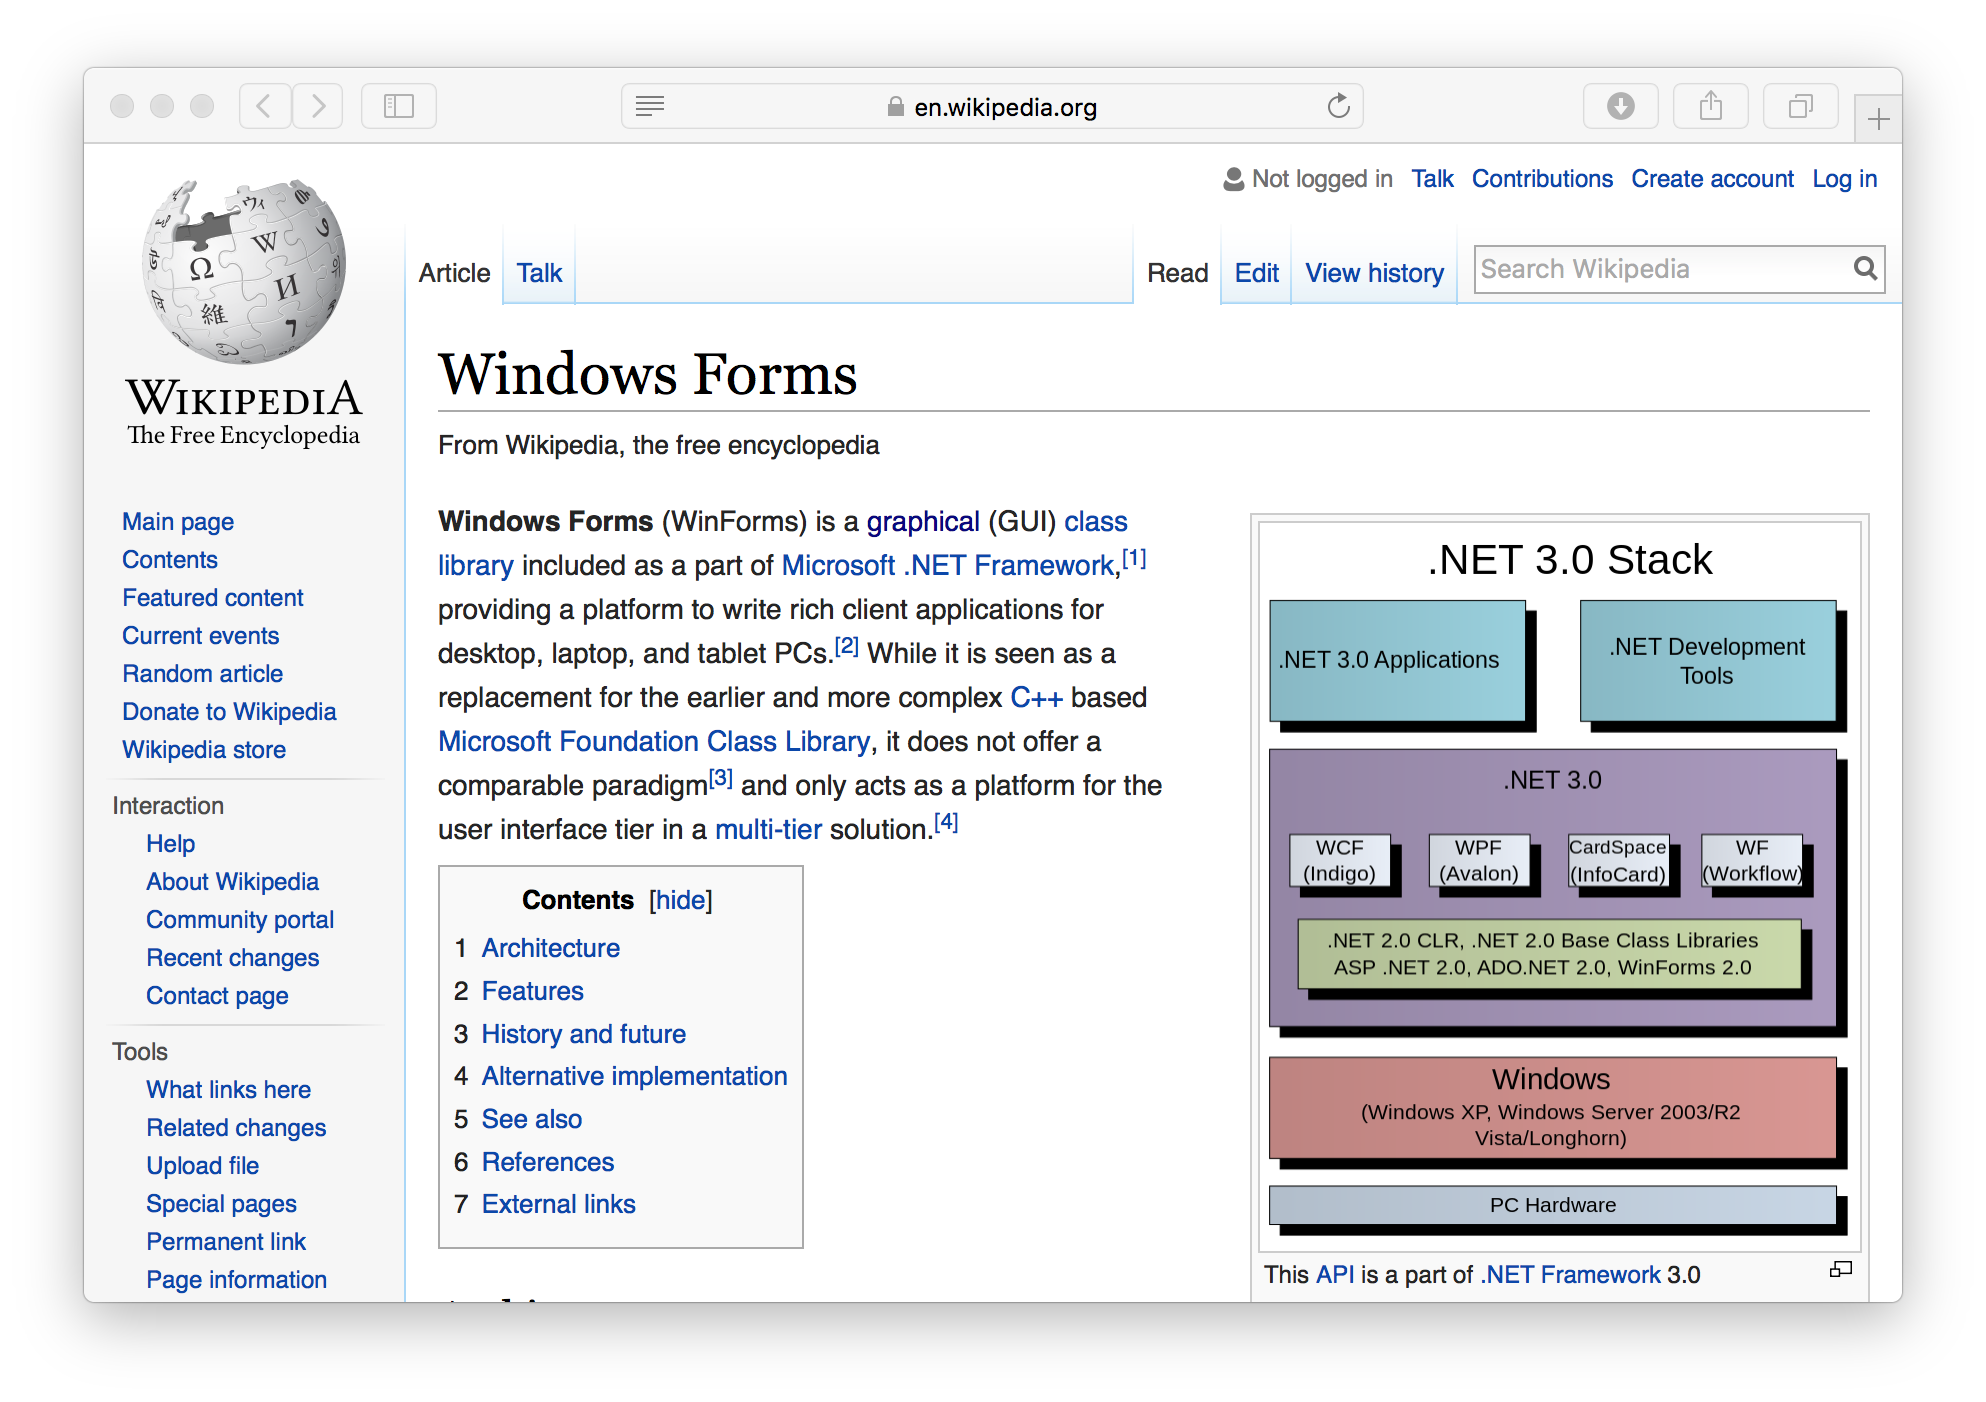
\includegraphics[width=0.6\textwidth]{safariWinForms}
  \caption{A web-browser is a graphical user interface for accessing a web-server and interacting with its services. Here the browser is showing the page \url{https://en.wikipedia.org/wiki/Windows_Forms} at time of writing.}
  \label{fig:safariGui}
\end{figure}
The program present information to the user in terms of text and images, and has areas that when activated by clicking with a mouse or similar allows the user to, e.g., go to other web-pages by type URL, to follow hyperlinks, and to generate new pages by entering search queries.

\section{Drawing primitives in Windows}
WinForms is based on two namespaces: \lstinline!System.Windows.Forms! and \lstinline!System.Drawing!. To start making a graphical display on the screen, the first thing to do is open a window, which acts as a reserved screen space for our output. With WinForms, this may be done as shown in Listing~\ref{winforms/openWindow}, and the result is shown in Figure~\ref{fig:openWindow}.
%
\fsCode{winforms/openWindow}{Create the window and turn over control to the operating system. Use \lstinline!win.Show()! on Microsoft Windows instead.}
%
\begin{figure}
  \centering
  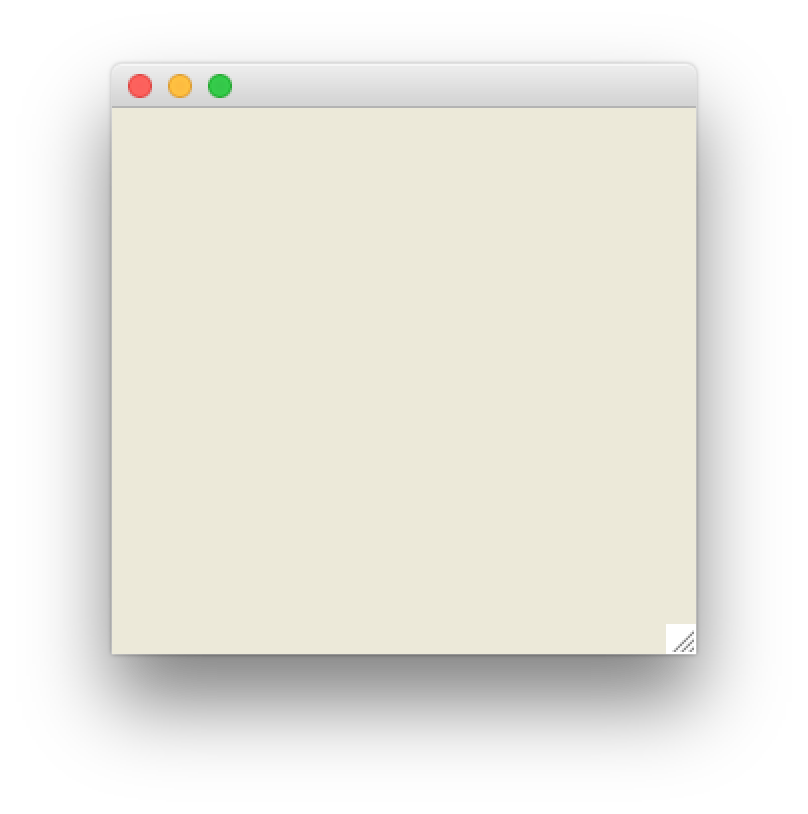
\includegraphics[width=0.6\textwidth]{openWindow}
  \caption{Result of running listing Listing~\ref{winforms/openWindow}.}
  \label{fig:openWindow}
\end{figure}
The \lstinline!new System.Windows.Forms.Form ()! creates an object (See Chapter~\ref{chap:oop}), but does not display the window on the screen. When the function \lstinline!System.Windows.Forms.Application.Run! is applied to the object, then the control is handed over to the WinForm's \idx{event-loop}, which continues until the window is closed by, e.g., pressing the icon designated by the operating system. On the mac OSX that is the red button in the top left corner of the window frame, and on Window it is the cross on the top right corner of the window frame.

The window, which WinForms calls a form, has a long list of \idx{methods} and \idx{properties}. E.g., the background color may be set by \lstinline!BackColor!, the title of the window may be set by \lstinline!Text!, and you may get and set the size of the window with the \lstinline!Size!. This is demonstrated in Listing
%
\fsCode{winforms/windowAttributes}{Create the window and changing its properties.}
%
\begin{figure}
  \centering
  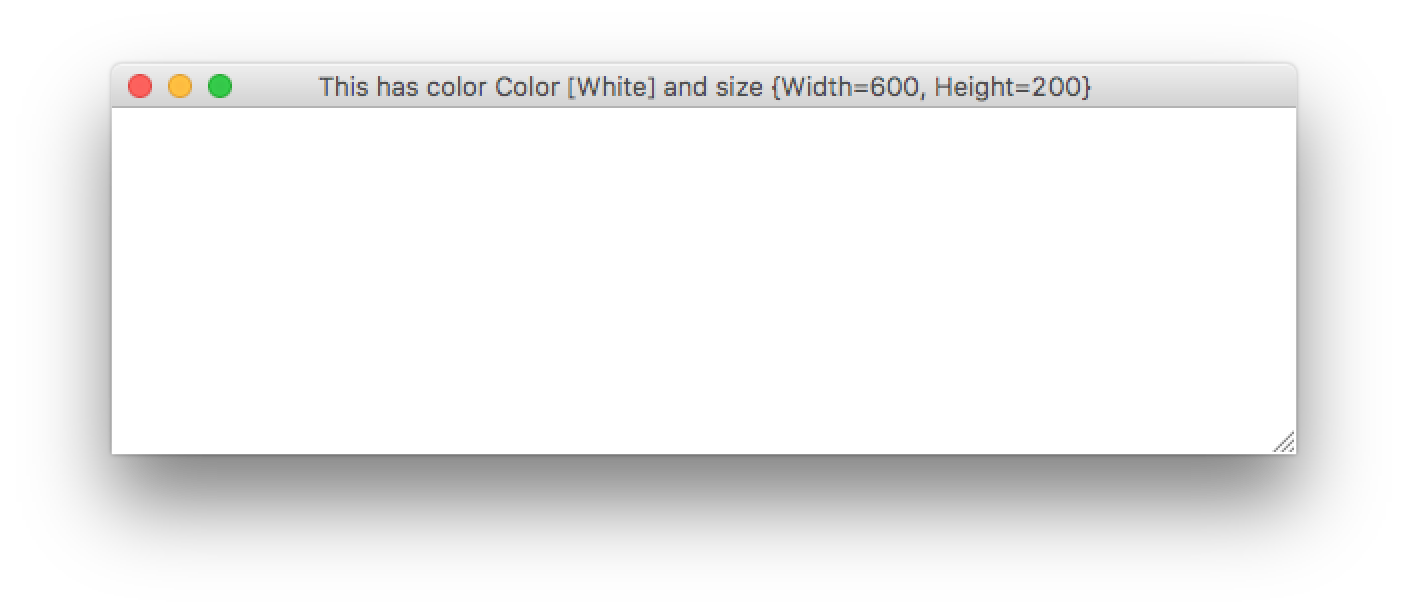
\includegraphics[width=0.6\textwidth]{windowAttributes}
  \caption{Result of running listing Listing~\ref{winforms/windowAttributes}.}
  \label{fig:openWindow}
\end{figure}
These properties have been programmed as \idx{accessors} implying that they may used as mutable variables. The \idx{\lstinline{System.Drawing.Color}} is a general structure for specifying colors as 4 channels: alpha, red, green, blue, where each channel is an 8 bit unsigned integer, where the alpha channel specifies the transparency of a color, where values 0--255 denotes the range of fully transparent to fully opaque, and the remaining channels denote the amount of red, green, and blue where 0 is none and 255 is full intensity. Any color may be created using the \lstinline!FromArgb! method, e.g., an opaque red is given by \lstinline!System.Drawing.Color.FromArgb (255, 255, 0, 0)!. There are also many build-in colors, e.g., the same red color is also a known color and may be obtained as \lstinline!System.Drawing.Color.Red!. For a given color, then the 4 alpha, red, green, and blue channel's values may be obtained as the \lstinline!A!, \lstinline!R!, \lstinline!G!, \lstinline!B!, see Listing~\ref{drawingColors}
%
\fs{drawingColors}{Defining colors and accessing their values.}
%
The \lstinline!System.Drawing.Size! is a general structure for specifying sizes as height and width pair of integers.

WinForms supports drawing of simple graphics primitives. Simple examples are \lstinline!System.Drawing.Pen! to specify the color to be drawn, \lstinline!System.Drawing.Point! to specify a pair of coordinates, and \lstinline!System.Drawing.Graphics.DrawLine!. \lstinline!DrawLine! is different than the previous examples since it must be related to a specific device, and it is typically accessed as an event. Displaying graphics in WinForms is performed as the reaction to an event. E.g., windows are created by the program, moved, minimized, occluded by other windows, resized, etc., by the user or the program, and each action may require that the content of the window is refreshed. Thus, we must create a function that WinForms can call, when it determines that the content needs to be redrawn. This is known as a \idx{call-back function}, and it is added to an existing form using the \lstinline!Paint.Add! function. As an example, consider the problem of draw a triangle in a window. For this we need to make a function that can draw a triangle not once, but any time WinForms determines it necessary to draw and redraw the triangle. Drawing is done with reference to a coordinate system. WinForms operates with several coordinate systems, the most important is the \idx{screen coordinates}. Screen coordinate $(x,y)$ have their origin in the top-left corner, and $x$ increases to the right, while $y$ increases down.\jon{Possibly something about client coordinates and world coordinates.} Thus, we may draw a triangle as demonstrated in Listing~\ref{winforms/triangle}.
%
\fsCode{winforms/triangle}{Create the window and changing its properties.}
%
\begin{figure}
  \centering
  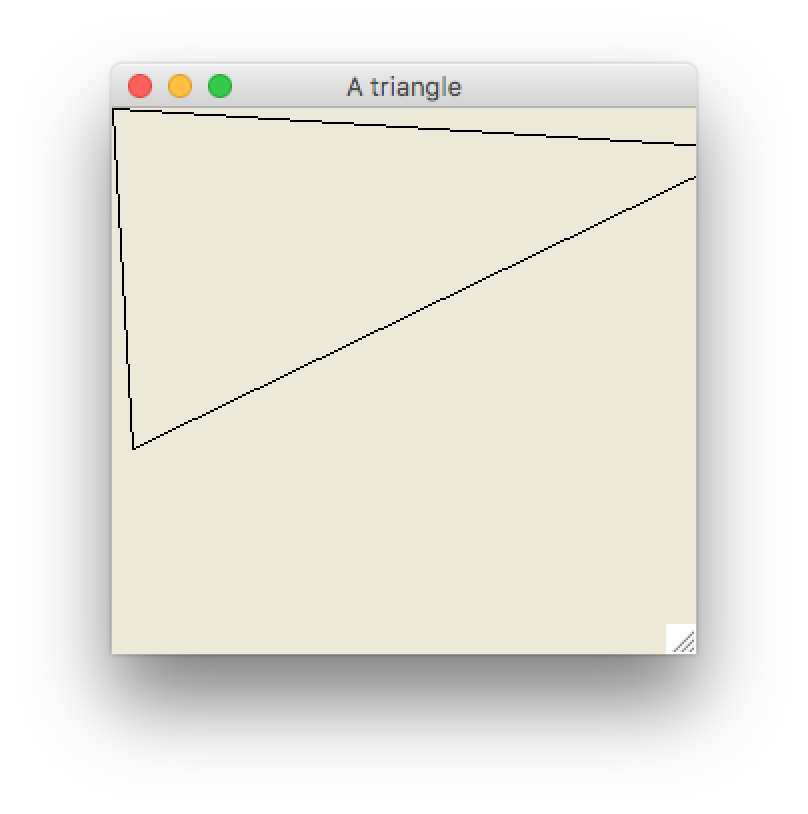
\includegraphics[width=0.6\textwidth]{triangle}
  \caption{Result of running listing Listing~\ref{winforms/triangle}.}
  \label{fig:triangle}
\end{figure}
A walk-through of the code is as follows: First we create an array of points and a pen color, then we create a pen and a window. The method for drawing the triangle is added as an anonymous function using the created window's \lstinline!Paint.Add! method. This function is to be called as a response to a paint event, and takes a \lstinline!PaintEventArgs! object, which includes the System.Drawing.Graphics object. Since this object will be related to a specific device, when \lstinline!Paint! is called then we may call the \lstinline!DrawLine! function to sequentially draw lines between our array of points. Finally, we hand the form to the event-loop, which as one of the earliest events will open the window and call the \lstinline!Paint! function we have associated with the form.

%
\fsCode{winforms/triangleOrganized}{Create the window and changing its properties.}
%
\begin{figure}
  \centering
  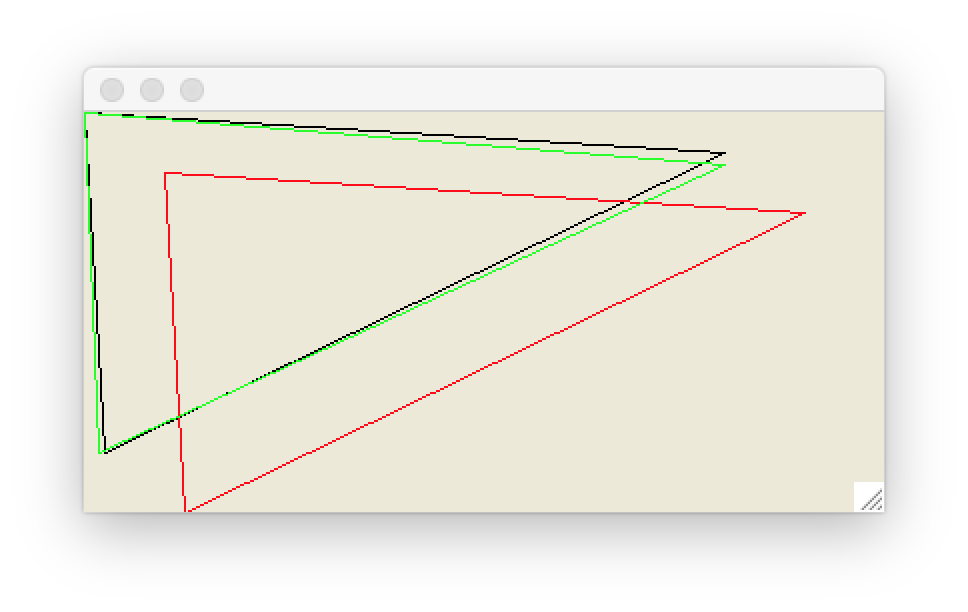
\includegraphics[width=0.6\textwidth]{triangleOrganized}
  \caption{Result of running listing Listing~\ref{winforms/triangleOrganized}.}
  \label{fig:triangleOrganized}
\end{figure}
\jon{requires the introduction of type declarations.}\jon{Remember to talk about pen width.}

%
\fsCode[numbers=left,numbersep=6pt,numberstyle=\scriptsize\color{white},lastline=42]{winforms/transformWindows}{Create the window and changing its properties: top part.}
\fsCode[numbers=left,numbersep=6pt,numberstyle=\scriptsize\color{white},firstnumber=44,firstline=44]{winforms/transformWindows}{Create the window and changing its properties: bottom part.}
%
\begin{figure}
  \centering
  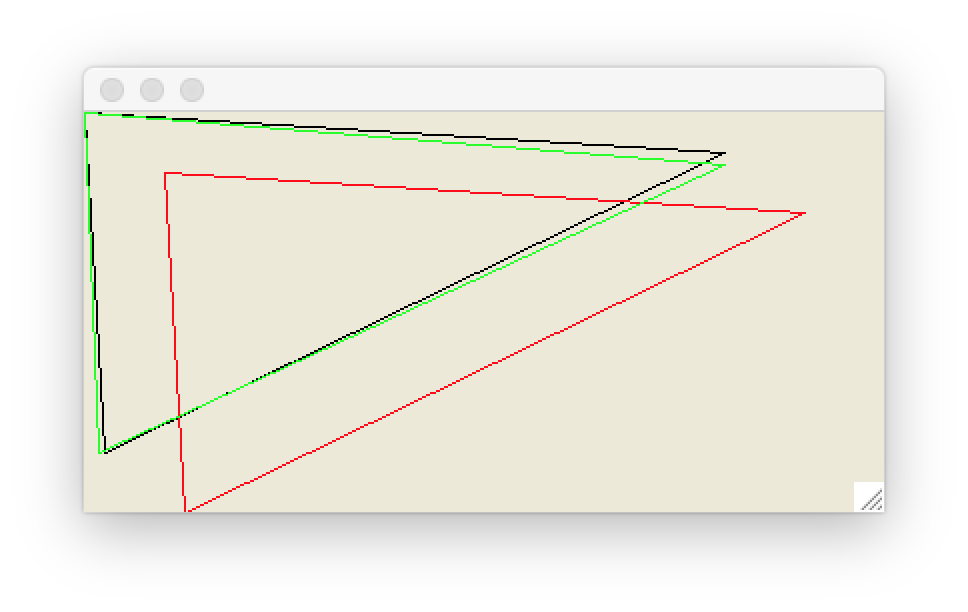
\includegraphics[width=0.6\textwidth]{transformWindows}
  \caption{Result of running listing Listing~\ref{winforms/transformWindows}.}
  \label{fig:transformWindow}
\end{figure}

\begin{problem}
  Given a triangle produce a Mandela drawing, where $n$ rotated versions of the triangle is drawn around its center of mass.
\end{problem}
%
\fsCode[numbers=left,numbersep=6pt,numberstyle=\scriptsize\color{white},firstnumber=44,firstline=44]{winforms/rotationalSymmetry}{Create the window and changing its properties.}
%
\begin{figure}
  \centering
  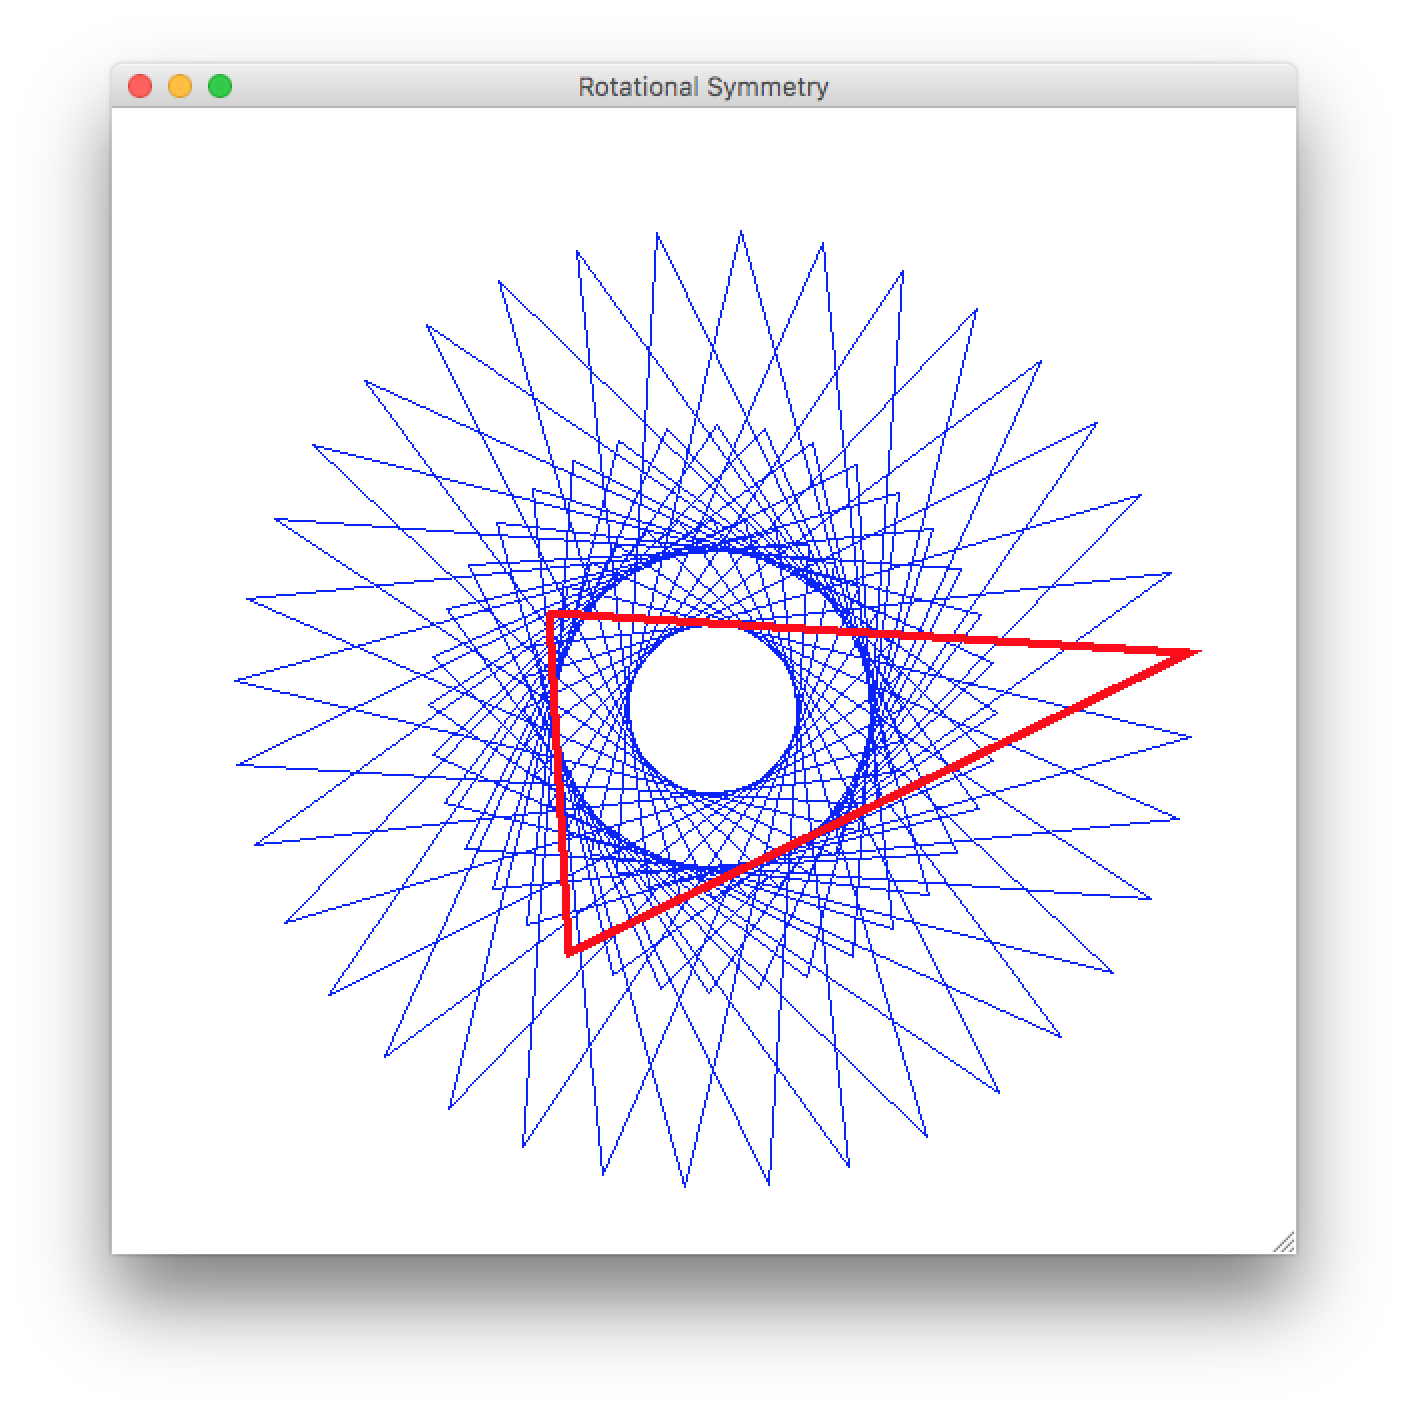
\includegraphics[width=0.8\textwidth]{rotationalSymmetry}
  \caption{Result of running listing Listing~\ref{winforms/rotationalSymmetry}.}
  \label{fig:rotationalSymmetry}
\end{figure}

\jon{Add other things to draw: filled stuff, clearing, circles, text}

\begin{table}
  \begin{center}
  \rowcolors{2}{oddRowColor}{evenRowColor}
    \begin{tabularx}{\linewidth}{|l|X|}
      \hline
      \rowcolor{headerRowColor}  Function & Description\\
      \hline
      \lstinline{DrawArc : Pen * Rectangle * Single * Single}
      &Draws an arc representing a portion of an ellipse specified by a Rectangle structure.\\
      \hline
      \lstinline{DrawBezier : Pen * Point * Point * Point * Point}	
      &Draws a Bézier spline defined by four Point structures.\\
      \hline
      \lstinline{DrawClosedCurve : Pen * Point[]}	
      &Draws a closed cardinal spline defined by an array of Point structures.\\
      \hline
      \lstinline{DrawCurve : Pen * Point[]}	
      &Draws a cardinal spline through a specified array of Point structures.\\
      \hline
      \lstinline{DrawEllipse : Pen * Rectangle}	
      &Draws an ellipse specified by a bounding Rectangle structure.\\
      \hline
      \lstinline{DrawImage : Image * Point[]}	
      &Draws the specified Image at the specified location and with the specified shape and size.\\
      \hline
      \lstinline{DrawLines : Pen * Point[]}	
      &Draws a series of line segments that connect an array of Point structures.\\
      \hline
      \lstinline{DrawPie : Pen * Rectangle * Single * Single}	
      &Draws a pie shape defined by an ellipse specified by a Rectangle structure and two radial lines.\\
      \hline
      \lstinline{DrawPolygon : Pen * Point[]}	
      &Draws a polygon defined by an array of Point structures.\\
      \hline
      \lstinline{DrawRectangles : Pen * Rectangle[]}	
      &Draws a series of rectangles specified by Rectangle structures.\\
      \hline
      \lstinline{DrawString : String * Font * Brush * PointF}	
      &Draws the specified text string at the specified location with the specified Brush and Font objects.\\
      \hline
      \lstinline{FillClosedCurve : Brush * Point[]}	
      &Fills the interior of a closed cardinal spline curve defined by an array of Point structures.\\
      \hline
      \lstinline{FillEllipse : Brush * Rectangle}	
      &Fills the interior of an ellipse defined by a bounding rectangle specified by a Rectangle structure.\\
      \hline
      \lstinline{FillPie : Brush * Rectangle * Single * Single}	
      &Fills the interior of a pie section defined by an ellipse specified by a RectangleF structure and two radial lines.\\
      \hline
      \lstinline{FillPolygon : Brush * Point[]}	
      &Fills the interior of a polygon defined by an array of points specified by Point structures.\\
      \hline
      \lstinline{FillRectangle : Brush * Rectangle}	
      &Fills the interior of a rectangle specified by a Rectangle structure.\\
      \hline
      \lstinline{FillRegion : Brush * Region}	
      &Fills the interior of a Region.\\
      \hline
    \end{tabularx}
  \end{center}
  \caption{Some methods of the \lstinline!System.IO.Path! class.}
  \label{tab:path}
\end{table}

\section{Programming intermezzo}
\begin{problem}
  Consider a curve consisting of piecewise straight lines all with the same length but with varying angles $0^{\circ}$, $90^{\circ}$, $180^{\circ}$, or $270^{\circ}$ w.r.t.\ the horisontal axis. To draw this curve we need 3 basic operations: Draw ($F$), turn right ($+$), and turn left ($-$). The turning is w.r.t.\ the present diretion. A Hilbert Curve is a spacefilling curve, which be expressed recursively as:
\begin{align}
  A &\rightarrow -BF+AFA+FB-\label{eq:hilbertA}\\
  B &\rightarrow +AF-BFB-FA+\label{eq:hilbertB}
\end{align}
starting with $A$. The order of the curve is the depth of the recursion, and to draw a 0'th order curve, we don't recurse at all, i.e., ignore all occurrences of the symbols $A$ and $B$ on the right-hand-side of \eqref{eq:hilbertA}, and get $-F+F+F-$. For the 1'st order curve, we recurse once, i.e., 
\begin{align*}
  A 
  \rightarrow &-BF+AFA+FB- \\
  \rightarrow &-(+AF-BFB-FA+)F\\
               &\quad+(-BF+AFA+FB-)F(-BF+AFA+FB-)\\
               &\qquad +F(+AF-BFB-FA+)-\\
  \rightarrow &AF-BFB-FA+FBF+AFA+FB-F-BF+AFA+FBF+AF-BFB-FA\\
  \rightarrow &F-F-F+FF+F+F-F-F+F+FF+F-F-F
\end{align*}
Make a program, that given an order produces an image of the Hilbert curve.
\end{problem}
%
\fsCode[numbers=left,numbersep=6pt,numberstyle=\scriptsize\color{white},firstnumber=44,firstline=44]{winforms/hilbert}{Create the window and changing its properties.}
%
\begin{figure}
  \centering
  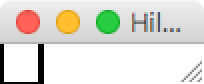
\includegraphics[width=0.45\textwidth]{hilbert1}
  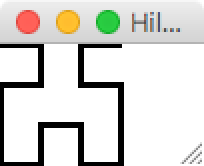
\includegraphics[width=0.45\textwidth]{hilbert2}
  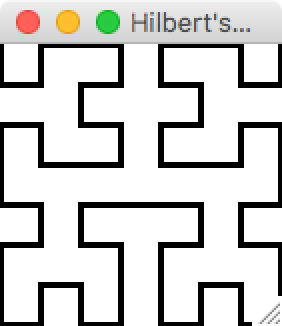
\includegraphics[width=0.45\textwidth]{hilbert3}
  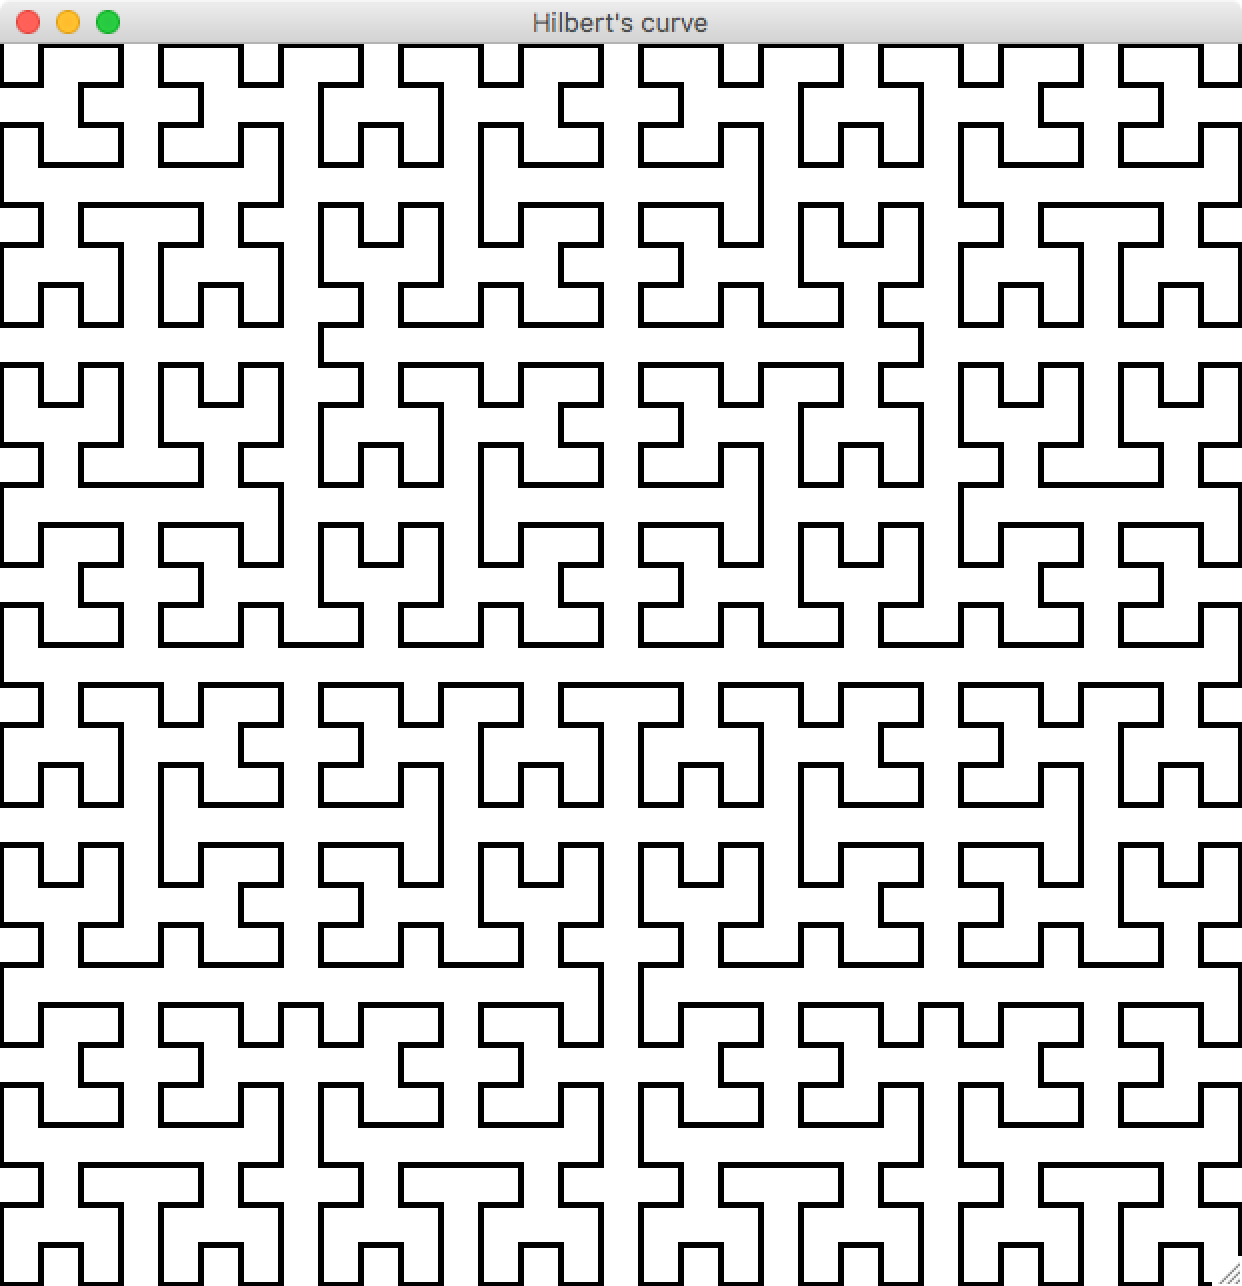
\includegraphics[width=0.45\textwidth]{hilbert5}
  \caption{Result of running listing Listing~\ref{winforms/hilbert}.}
  \label{fig:hilbert1}
\end{figure}

%
\fsCode{winforms/windowEvents}{Catching window, mouse, and keyboard events..}
%

\section{Buttons and stuff}

%
\fsCode{winforms/buttonControl}{Create the button and an event.}
%
\begin{figure}
  \centering
  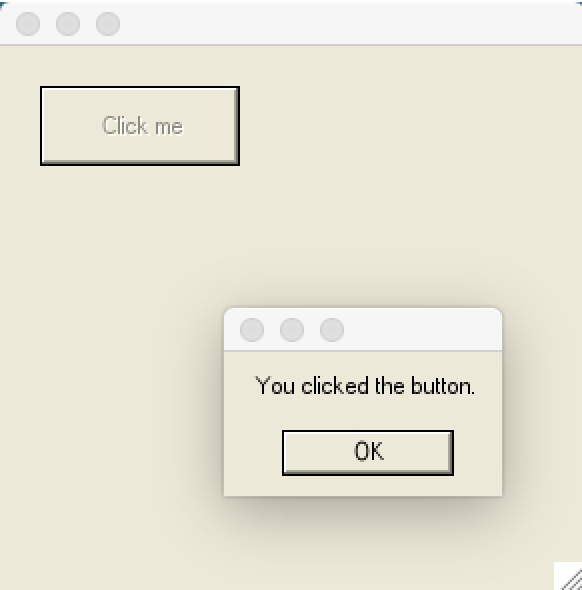
\includegraphics[width=0.6\textwidth]{buttonControl}
  \caption{Result of running listing Listing~\ref{winforms/buttonControl}.}
  \label{fig:buttonControl}
\end{figure}

%
\fsCode{winforms/panel}{Create a panel, label, text input controls.}
%
\begin{figure}
  \centering
  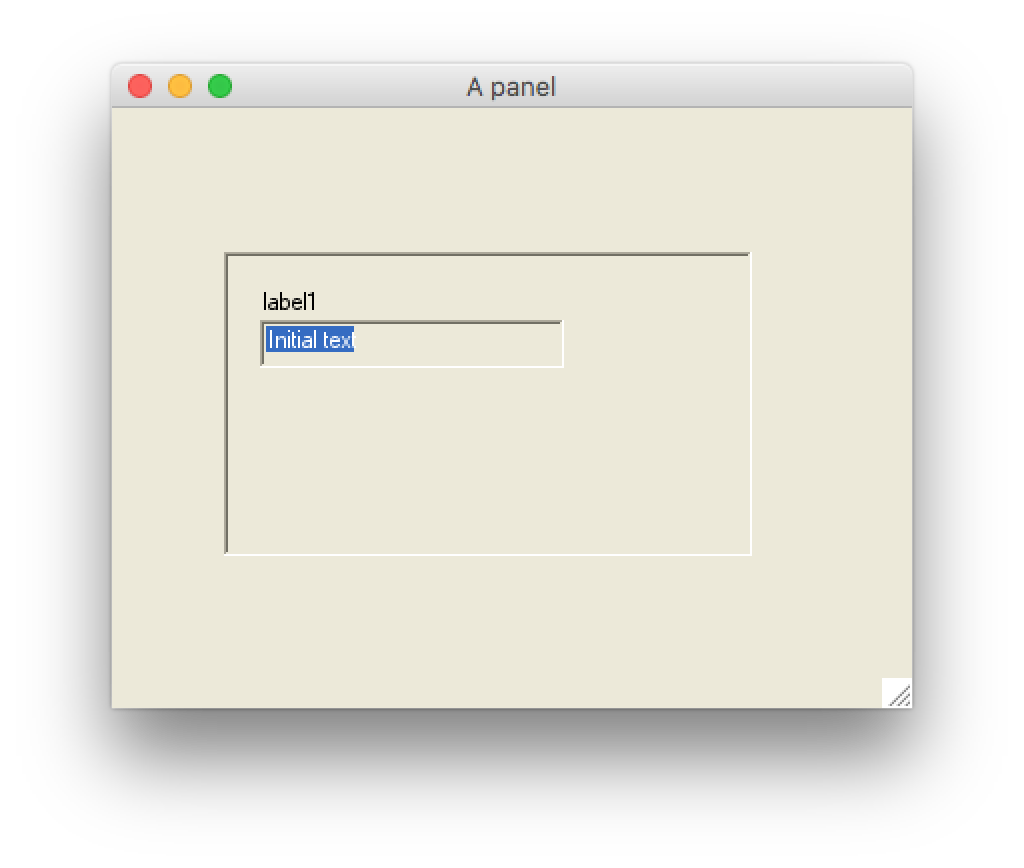
\includegraphics[width=0.6\textwidth]{panel}
  \caption{Result of running listing Listing~\ref{winforms/panel}.}
  \label{fig:panel}
\end{figure}

%
\fsCode[lastline=42]{winforms/flowLayoutPanel}{Create a flowLayoutPanel, with checkbox and radiobuttons.}
%
%
\fsCode[firstnumber=43,firstline=43,lastline=87]{winforms/flowLayoutPanel}{Create a flowLayoutPanel, with checkbox and radiobuttons.}
%
%
\fsCode[firstnumber=88,firstline=88]{winforms/flowLayoutPanel}{Create a flowLayoutPanel, with checkbox and radiobuttons.}
%
\begin{figure}
  \centering
  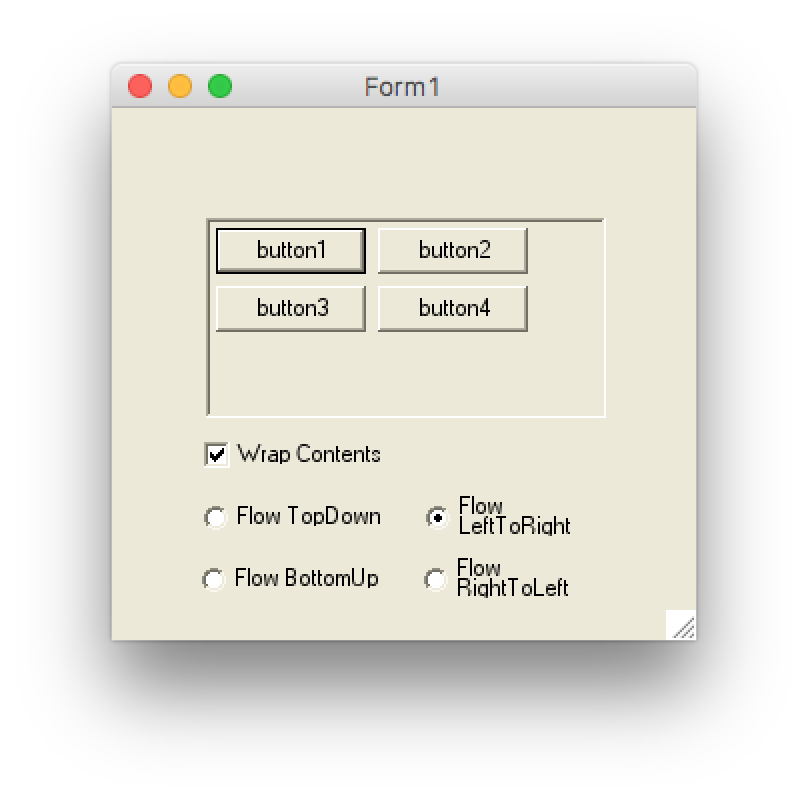
\includegraphics[width=0.6\textwidth]{flowLayoutPanel}
  \caption{Result of running listing Listing~\ref{winforms/flowLayoutPanel}.}
  \label{fig:flowLayoutPanel}
\end{figure}



\jon{\lstinline!Click.Add! expects a function \lstinline!System.EventArgs -> unit! therfore the \lstinline!ignore! function.}

\begin{table}
  \begin{center}
  \rowcolors{2}{oddRowColor}{evenRowColor}
    \begin{tabularx}{\linewidth}{|l|X|}
      \hline
      \rowcolor{headerRowColor}  Function & Description\\
      \hline
      \lstinline{DataGridView}
      &Display data on a table.\\
      \hline
      \lstinline{TextBox}
      &Display editable text.\\
      \hline
      \lstinline{Label}
      &Display text.\\
      \hline
      \lstinline{LinkLabel}
      &Display clickable text.\\
      \hline
      \lstinline{ProgressBar}
      &Display the current progress as a bar.\\
      \hline
      \lstinline{WebBrwoser}
      &Enable navigation of the web.\\
      \hline
      \lstinline{CheckedListBox}
      &Display a scrollable check box list.\\
      \hline
      \lstinline{ComboBox}
      &Display a drop-down list.\\
      \hline
      \lstinline{ListBox}
      &Display a list of text and icons.\\
      \hline
      \lstinline{PictureBox}
      &Display a bitmap image\\
      \hline
      \lstinline{CheckBox}
      &Display a checkbox and a label of text.\\
      \hline
      \lstinline{RadioButton}
      &Display an on-off radio button\\
      \hline
      \lstinline{TrackBar}
      &Enable the user to input value by moving a cursor on a slider bar\\
      \hline
      \lstinline{DateTimePicker}
      &Enable the user to select a date from a graphical calendar\\
      \hline
      \lstinline{ColorDialogue}
      &Enable the user to pick a color\\
      \hline
      \lstinline{FontDialog}
      &Enable the user to pick a font and its attributes\\
      \hline
      \lstinline{OpenFileDialog}
      &Enable the user to navigate the file system and select a file..\\
      \hline
      \lstinline{PrintDialog}
      &Enable the user to select a printer and its attributes.\\
      \hline
      \lstinline{SaveDialog}
      &Enable the user to navigate the file system and specify a filename.\\
      \hline
      \lstinline{MenuStrip}
      &Allow the user to choose from a custom menu\\
      \hline
      \lstinline{Button}
      &Display a clickable button with text\\
      \hline
      \lstinline{Tooltip}
      &Briefly display a pop-up window, when the user rests the pointer on the control\\
      \hline
      \lstinline{SoundPlayer}
      &Play sounds in the \lstinline{.wav} format.\\
      \hline
    \end{tabularx}
  \end{center}
  \caption{Some controls available in WinForms.}
  \label{tab:controls}
\end{table}

\begin{table}
  \begin{center}
  \rowcolors{2}{oddRowColor}{evenRowColor}
    \begin{tabularx}{\linewidth}{|l|X|}
      \hline
      \rowcolor{headerRowColor}  Function & Description\\
      \hline
      \lstinline{Panel}
      &Groups a set of controls in a scrollable frame.\\
      \hline
      \lstinline{GroupBox}
      &Group a set of controls in a non-scrollable frame.\\
      \hline
      \lstinline{TabControl}
      &Group controls in tabpages, A tabpage is selected by clicking on its tab.\\
      \hline
      \lstinline{SplitContainer}
      &Group controls into two resizable panels.\\
      \hline
      \lstinline{TableLayoutPanel}
      &Group controls into a grid.\\
      \hline
      \lstinline{FlowLayoutPanel}
      &Group controls into a set of flowable panels. The panels may flow horizontally or vertically as a response to window resizing.\\
      \hline
    \end{tabularx}
  \end{center}
  \caption{Some controls for grouping other controls.}
  \label{tab:controlGroups}
\end{table}

\dots

%%% Local Variables:
%%% TeX-master: "fsharpNotes"
%%% End:


\documentclass[fsharpnotes.tex]{subfiles}
\graphicspath{ {./figures/} }

\begin{document}
\chapter{Imperative programming}

\section{Introduction}
\idx[imperative programming]{Imperativ programming} focusses on how a problem is to be solved as a list of \idx[statement]{statements} and and a set of \idx{states}, where states may change over time. An example is a baking recipe, e.g., 
  \begin{enumerate}
  \item Mix yeast with water 
  \item Stir in salt, oil, and flour 
  \item Knead until the dough has a smooth surface 
  \item Let the dough rise until it has double size 
  \item Shape dough into a loaf 
  \item Let the loaf rise until double size 
  \item Bake in oven until the bread is golden brown
  \end{enumerate}
Each line in this example consists of one or more statements that are to be executed, and while executing them states such as size of the dough, color of the bread changes, and some execution will halt execution until certain conditions of these states are fulfilled, e.g., the bread will not be put into the oven for baking before it has risen sufficiently.

Statements may be grouped into procedures, and structuring imperative programs heavily into procedures is called \idx{Procedural programming}, which is sometimes considered as a separate paradigm from imperative programming. \idx[object-oriented programming]{Object-oriented programming} is an extension of imperative programming, where statements and states are grouped into classes and will be treated elsewhere.

Almost all computer hardware is designed for \idx{machine code}, which is a common term used for many low-level computer programming language, and almost all machine langues follow the imperative programming paradigm. 

  \idx{Functional programming} may be considered a subset of imperative programming, in the sense that functional programming does not include the concept of a state, or one may think of functional programming as only have one unchanging state. Functional programming has also a bigger focus on what should be solved, by declaring rules but not explicitly listing statements describing how these rules should be combined and executed in order to solve a given problem. Functional programming will be treated elsewhere.


\section{Generating random texts}
\subsection{0'th order statistics}
\fs{randomTextOrder0}{}

\subsection{1'th order statistics}
\fs{randomTextOrder1}{}
\end{document}
%%% Local Variables:
%%% TeX-master: "fsharpNotes"
%%% End:


\part{Declarative programming}
\label{part:declarative}

%%% Local Variables:
%%% TeX-master: "fsharpNotes"
%%% End:


\documentclass[fsharpnotes.tex]{subfiles}
\graphicspath{ {./figures/} }

\begin{document}
\chapter{Sequences and computation expressions}
\label{chap:sequences}\jon{possibly add maps and sets as well.}
\section{Sequences}
\label{sec:sequences}
Sequences are lists, where the elements are build as needed. Examples are\jon{Mono does not support specification Spec-4.0 Section 6.3.11, seq {comp-expr}, in the form seq {3} or seq {3; 4}.}
%
\fsOutput{seqExample}{Creating sequences by range explicitly stating elements, a range expressions, a computation expression, and an infinite computation expression}
%
Sequences are built using the following subset of the general syntax,
\begin{lstlisting}[language=ebnf]
range-exp = expr ".." expr [".." expr]
comp-expr =
  "let" pat "=" expr "in" comp-expr
  | "use" pat = expr "in" comp-expr
  | ("yield" | "yield!") expr
  | "if" expr "then" comp-expr ["else" comp-expr]
  | "match" expr "with" comp-rules
  | "try" comp-expr "with" comp-rules
  | "try" comp-expr "finally" expr
  | "while" expr "do" expr ["done"]
  | "for" ident "=" expr "to" expr "do" comp-expr ["done"]
  | "for" pat "in" expr-or-range-expr "do" comp-expr ["done"]
  | comp-expr ";" comp-expr
short-comp-expr = "for" pat "in" (expr | range-expr) "->" expr
comp-or-range-expr = comp-expr| short-comp-expr | range-expr
comp-rule = pat pattern-guardopt "->" comp-expr
comp-rules = comp-rule | comp-rule '|' comp-rules
expr = ... 
  | "seq" "{" comp-or-range-expr "}" (* computation expression *)
  | ...
\end{lstlisting}
%
Sequence may be defined using simple range expressions but most often are defined as a small program, that generates values with the \keyword{yield} keyword or \keyword{yield!} keyword. The \keyword{yield!} is called \idx{yield bang}, and appends a sequence instead of adding a sequence as an element. Thus, \lstinline!seq {3; 5}! is not permitted, but \lstinline!seq {yield 3; yield 5}! and \lstinline|seq {yield! (seq {yield 3; yield 5})}| are, both creating \lstinline!seq<int> = seq [3; 5]!, i.e., a sequence of integers. Most often computation expressions are used to produced members that are not just ranges, but more complicated expressions of ranges, e.g., \lstinline!c! in the example. Sequences may even in principle be infinitely long, e.g., \lstinline!d!. Calculating the complete sequence at the point of definition is impossible due to lack of memory, as is accessing all its elements due to lack of time. But infinite sequences are still very useful, e.g., identifier \lstinline!d! illustrates the parametrization of a circle, which is an infinite domain, and any index will be converted to the equivalent 60th degree angle in radians. F\# warns against recursive values, as defined in the example, since it will check the soundness of the value at runtime rather than at compile-time. The warning can be removed by adding \lstinline!#nowarn "40"! in the script or \lstinline!--nowarn:40! as argument to \lstinline[language=console]!fsharpi! or \lstinline[language=console]!fsharpc!.

Sequences are generalisations of lists and arrays, and functions taking sequences as argument may equally take lists and arrays as argument. Sequences do not have many built-in operators, but a rich collection of functions in the \lstinline!Collections.Seq!. E.g.,\idxss{Seq.item}\idxss{Seq.take}
%
\fsOutput{seqIndexing}{Index a sequence with \lstinline!Seq.item! and \lstinline!Seq.take!}
%
which as usual index from 0 and will cast an exception, if indexing is out of range for the sequence. 

That sequences really are programs rather than values can be seen by the following example,
%
\fsOutput{seqDelayedEval}{Sequences elements are first evaluated, when needed.}
%
In the example, we see that the \lstinline!printfn! function embedded in the definition is first executed, when the 3rd item is requested.

\jon{Mono, missing support for Spec-4.0 Chapter 6, \lstinline!do!-\lstinline!in! in sequences. E.g., \lstinline!seq {let _ = printfn "hej" in yield 3}! is ok, but \lstinline!seq {do printfn "hej" in yield 3}! not. One could argue, that computation expression is the framework and that it is the seq implementation, which does not provide full access to the framework. but this is confusing, since seq gets special attention in the specification.}

The only difference between computation expression's programming constructs and the similar regular expressions constructs is that they must return a value with the \keyword{yield} or \keyword{yield!} keywords.\jon{Mono implements if-elif-else, but this is not in the specification.} The \keyword{try}-keyword constructions will be discussed in \Cref{chap:errors}, and the \keyword{use}-keyword is a variant of \keyword{let} but used in asynchronous computations, which will not be treated here.

  % "let" pat "=" expr "in" comp-expr
  % | "use" pat = expr "in" comp-expr
  % | ("yield" | "yield!") expr
  % | "if" expr "then" comp-expr ["else" comp-expr]
  % | "match" expr "with" comp-rules
  % | "try" comp-expr "with" comp-rules
  % | "try" comp-expr "finally" expr
  % | "while" expr "do" expr ["done"]
  % | "for" ident "=" expr "to" expr "do" comp-expr ["done"]
  % | "for" pat "in" expr-or-range-expr "do" comp-expr ["done"]
  % | comp-expr ";" comp-expr

Infinite sequences is a useful concept in many programs and may be generated in a number of ways. E.g., to generate a repeated sequence, we could use recursive value definition, a computation expression, a recursive function, or the \lstinline!Seq! module. Using a recursive value definition,
%
\fs{seqInfinteValue2}{Recursive value definitions gives a warning.  Compare with Listing\ref{seqInfinteValue}, \ref{seqInfinteFunction}, and \ref{seqInitInfinite}.}
%
F\# warns against using recursive values, since it will check the soundness of the value at runtime rather than at compile-time. The warning can be removed by adding \lstinline!#nowarn "40"! in the script or \lstinline!--nowarn:40! as argument to \lstinline[language=console]!fsharpi! or \lstinline[language=console]!fsharpc!, but \advice{warnings are messages from the designers of F\# that your program is non-optimal, and you should avoid structures that throw warnings instead of relying on \lstinline{\#nowarn} and similar constructions.} Instead we may create an infinite loop using the \keyword{while}-\keyword{do} computation expression, as
%
\fs{seqInfinteValue}{Infinite value definition without recursion nor warning.  Compare with \Cref{seqInfinteValue2}, \ref{seqInfinteFunction}, and\ref{seqInitInfinite}.}
%
or alternatively define a recursive function,
%
\fs{seqInfinteFunction}{Recursive function definitions gives no a warning.  Compare with \Cref{seqInfinteValue2}, \ref{seqInfinteValue}, and \ref{seqInitInfinite}.}
%
Infinite expressions have built-in support through the \lstinline!Seq! module using \idxss{Seq.initInfinite},
%
\fs{seqInitInfinite}{Using \lstinline{Seq.initInfinte} and a function to generate an infinte sequence. Compare with \Cref{seqInfinteValue2}, \ref{seqInfinteValue}, and \ref{seqInfinteFunction}.}
%
which takes a function as argument. Here we have used currying, i.e., \lstinline!get items! is a function that takes on variable and returns a value. The use of the remainder operator makes the example rather contrived, since it might have been simpler to use the \lstinline!get! indexing function directly.

Sequences are easily converted to and from lists and arrays as,\idxss{Seq.toList}\idxss{Seq.toArray}
%
\fs{seqConversion}{Conversion between sequences and lists and arrays using the \lstinline!List! module.}
%
There are quite a number of built-in functions for sequences many which will be discussed in \Cref{chap:collection}.
 
Lists and arrays may be created from sequences through the short-hand notation called \idx[list sequence expression]{list and array sequence expressions}\idxss{array sequence expressions},
\begin{lstlisting}[language=ebnf]
expr = ... 
  | "[" (... | comp-expr | short-comp-expr | ...) "]" (* list sequence expression *)
  | "[|" (.. | comp-expr | short-comp-expr | ...) "|]" (* array sequence expression *)
  | ...
\end{lstlisting}
which implicitly creates the corresponding expression and return the result as a list or array.

% *****

% \fs{arrayJaggedCompExpr}{}
% Indexing arrays of arrays is done sequentially, in the sense that in the above example, the number of outer arrays is \lstinline|a.Length|,  \lstinline|a.[i]| is the i'th array, the length of the i'th array is \lstinline|a.[i].Length|, and the j'th element of the i'th array is thus \lstinline|a.[i].[j]|. Often 2 dimensional square arrays are used, which can be implemented as a jagged array as,
% \fs{arrayJaggedSquareCompExpr}{}
% In fact, square arrays of dimensions 2 to 4 are so common that F\# has built-in modules for their support. In the following describe Array2D. The workings of Array3D and Array4D are very similar. An example of creating the same 2 dimensional array as above but as an \texttt{Array2D} is,
% \fs{array2DCompExpr}{}
% Notice that the indexing uses a slightly different notation '\lstinline|[,]|' and the length functions are also slightly different. The statement \lstinline|A.Length| would return the total number of elements in the array, in this case 12.


\end{document}
%%% Local Variables:
%%% TeX-master: "fsharpNotes"
%%% End:


\chapter{Patterns}
\label{chap:patterns}
\section{Pattern matching}
Conditional expressions are so common that a short-hand notation called \idx{pattern matching} is available in F\#. For the 
Consider the task,
\begin{problem}
  Write a function that given $n$ writes the sentence, ``I have n apple(s)'', where the plural 's' is added appropriately.
\end{problem}
For this we need to test on $n$'s size, and one option is to use conditional expressions like,
%
\fs{matchWith}{Using the \keyword{match}-keyword{with} programming construct to vary calculation based on the input value.}
%
Here the \idx{\keyword{match}}-\idx{\keyword{with}} keywords starts a sequence of conditions separated by the \lexeme{|} lexeme, where the default operator is the \lexeme{=} comparison operator, but where others can be used with the \idx{\keyword{when}}. The syntax of \keyword{match} expressions is,
\begin{lstlisting}[language=ebnf]
pat = const | "_" | ...
guard = "when" expr
rule = pat [guard] -> expr
rules = "|" rule | "|" rule rules (* first "|'' is optional' *)
expr = ... 
  | "match" expr "with" rules (* match expression *)
  | "function" rules (* matching function expression *)
  | ...
\end{lstlisting}
As for conditional expressions, the rules are treated sequentially from first to last, and the expression following the first rule with a true condition is the the result of the entire expression. The rules are versatile in their possible expression, e.g., the line \lstinline!| 1 -> "I have no apples"! is equivalent to \lstinline!elif n < 1 then "I have no apples"|, and the \lstinline!| \_ -> "I have " + (string n) + " apples"!, matches the \lstinline!else "I have " + (string n) + " apples"!, since the \lexeme{_} lexeme is a wildcard pattern matching anything. Finally, the first rule is a guarded rule indicated by the \keyword{when} keyword, \lstinline!i when i < 0 -> "I owe " + (string -i) + " apples"!. It uses the optional disregard of the \lexeme{|} lexeme and is equivalent to \lstinline!if n < 0 then "I owe " + (string -n) + " apples"!. Guarded rules can be any rules, and here we used the identifier \lstinline!i! meaning \lstinline!let i = n in if i < 0 then ...!, i.e., \lstinline!n! is renamed. One way to think of guarded expressions is that \lstinline!i when i < 0! is a set, and the condition is on \lstinline!n! being part of the set or not. 

Using lightweight syntax, the rules may be put on separate lines but must start in the column, where the \keyword{match} starts or greater.\spec{Spec-4.0 weirdness: Offside rule for match is different for function.} Match with can only take one identifier, but this can be tuples for matching with combinations of identifiers, see Chapter~\ref{chap:lists} for more on tuples. A \keyword{match} expression is general but is most often seen as the initial part of a function definition. This is so common, that F\# has a special syntax integrating function definitions and match with expressions using the \idx{\keyword{function}} keyword,
%
\fs{functionKeyword}{Function definition and \keyword{match} expressions are integrated using the \keyword{function} keyword. Compare with Listing~\ref{matchWith}}
%
Comparing with Listing~\ref{matchWith} notice that the function definition does not explicitly name an argument but assumes one, following the \keyword{function} follows immediately the rules, and the wildcard pattern \lexeme{_} is replaced with an identifier without any guards, which thus matches everything. Replacing the wildcard pattern with a name has the advantage that this name can be used locally in the expression belonging to this rule, i.e., it acts as a \lstinline!let n = ! on the implicit argument of the function. Implicit arguments makes the code hard to read and, thus \advice{the use of function definitions with the keyword \keyword{function} should be avoided.}\jon{Should we extend this with a more detail description of possiblities from Spec-4.0 Chapter 7?}

%%% Local Variables:
%%% TeX-master: "fsharpNotes"
%%% End:


\documentclass[fsharpNotes.tex]{subfiles}
\graphicspath{ {./figures/} }

\begin{document}
\chapter{Types and measures}
\section{Unit of Measure}
\label{sec:measures}
 F\# allows for assigning \idx{unit of measure} to the following types,
\begin{quote}
  \mbox{\lstinline{sbyte},}
  \mbox{\lstinline{int},}
  \mbox{\lstinline{int16},}
  \mbox{\lstinline{int32},}
  \mbox{\lstinline{int64},}
  \mbox{\lstinline{single},}
  \mbox{\lstinline{float32},}
  \mbox{\lstinline{float},} and
  \mbox{\lstinline{decimal}.}
\end{quote}
by using the syntax,
%
\begin{lstlisting}[language=EBNF]
"[<Measure>] type" unit-name [ "=" unit-expr ]
\end{lstlisting}
%
and then use \lstinline[language=EBNF]|"<" unit-name ">"| as suffix for literals. E.g., defining unit of measure 'm' and 's', then we can make calculations like,
%
\begin{lstlisting}[language=fsharp,caption={fsharpi, floating point and integer numbers may be assigned unit of measures.}]
> [<Measure>] type m
- [<Measure>] type s 
- let a = 3<m/s^2>
- let b = a * 10<s>
- let c = 4 * b;;

[<Measure>]
type m
[<Measure>]
type s
val a : int<m/s ^ 2> = 3
val b : int<m/s> = 30
val c : int<m/s> = 120
\end{lstlisting}
However, if we mixup unit of measures under addition, then we get an error,
%
\begin{lstlisting}[language=fsharp,caption={fsharpi, unit of measures adds an extra layer of types for syntax checking at compile time.}]
> [<Measure>] type m 
- [<Measure>] type s 
- let a = 1<m>
- let b = 1<s>
- let c = a + b;;

  let c = a + b;;
  ------------^

/Users/sporring/repositories/fsharpNotes/stdin(63,13): error FS0001: The unit of measure 's' does not match the unit of measure 'm'
\end{lstlisting}
Unit of measures allow for \lexeme{*}, \lexeme{/}, and \lexeme{^}\jon{Spec-4.0: this notation is inconsistent with \texttt{**} for float exponentiation.} for multiplication, division and exponentiation. Values with units can be casted to \idx{unit-less} values by casting, and back again by multiplication as,
%
\begin{lstlisting}[language=fsharp,caption={fsharpi, typecasting unit of measures.}]
> [<Measure>] type m      
- let a = 2<m>            
- let b = int a           
- let c = b * 1<m>;;

[<Measure>]
type m
val a : int<m> = 2
val b : int = 2
val c : int<m> = 2
\end{lstlisting}
Compound symbols can be declared as,
%
\begin{lstlisting}[language=fsharp,caption={fsharpi, aggregated unit of measures.}]
> [<Measure>] type s         
- [<Measure>] type m
- [<Measure>] type kg
- [<Measure>] type N = kg * m / s^2;;

[<Measure>]
type s
[<Measure>]
type m
[<Measure>]
type kg
[<Measure>]
type N = kg m/s ^ 2
\end{lstlisting}
For fans of the metric system there is the International System of Units, and these are built-in in \lstinline|Microsoft.FSharp.Data.UnitSystems.SI.UnitSymbols| and give in \Cref{tab:siUnits}.
\begin{table}
  \centering
  \begin{tabularx}{0.75\linewidth}{|l|X|}
    \hline
    Unit & Description \\
    \hline
    \lstinline|A| & Ampere, unit of electric current.\\
    \lstinline|Bq|&Becquerel, unit of radioactivity.\\
    \lstinline|C|&Coulomb, unit of electric charge, amount of electricity.\\
    \lstinline|cd|&Candela, unit of luminous intensity.\\
    \lstinline|F|&Farad, unit of capacitance.\\
    \lstinline|Gy|&Gray, unit of an absorbed dose of radiation.\\
    \lstinline|H|&Henry, unit of inductance.\\
    \lstinline|Hz|&Hertz, unit of frequency.\\
    \lstinline|J|&Joule, unit of energy, work, amount of heat.\\
    \lstinline|K|&Kelvin, unit of thermodynamic (absolute) temperature.\\
    \lstinline|kat|&Katal, unit of catalytic activity.\\
    \lstinline|kg|&Kilogram, unit of mass.\\
    \lstinline|lm|&Lumen, unit of luminous flux.\\
    \lstinline|lx|&Lux, unit of illuminance.\\
    \lstinline|m|&Metre, unit of length.\\
    \lstinline|mol|&Mole, unit of an amount of a substance.\\
    \lstinline|N|&Newton, unit of force.\\
    \lstinline|ohm|&Unitnames.o SI unit of electric resistance.\\
    \lstinline|Pa|&Pascal, unit of pressure, stress.\\
    \lstinline|s|&Second, unit of time.\\
    \lstinline|S|&Siemens, unit of electric conductance.\\
    \lstinline|Sv|&Sievert, unit of dose equivalent.\\
    \lstinline|T|&Tesla, unit of magnetic flux density.\\
    \lstinline|V|&Volt, unit of electric potential difference, electromotive force.\\
    \lstinline|W|&Watt, unit of power, radiant flux.\\
    \lstinline|Wb|&Weber, unit of magnetic flux.\\
    \hline
  \end{tabularx}
  \caption{International System of Units.}
  \label{tab:siUnits}
\end{table}
Hence, using the predefined unit of seconds, we may write,
%
\begin{lstlisting}[language=fsharp,caption={fsharpi, SI unit of measures are built-in.}]
> let a = 10.0<Microsoft.FSharp.Data.UnitSystems.SI.UnitSymbols.s>;;

val a : float<Data.UnitSystems.SI.UnitSymbols.s> = 10.0
\end{lstlisting}
To make the use of these predefined symbols easier, we can import them into the present scope by the \idx{\keyword{open}} keyword,
%
\begin{lstlisting}[language=fsharp,caption={fsharpi, simpler syntax by importing, but beware of namespace pollution.}]
> open Microsoft.FSharp.Data.UnitSystems.SI.UnitSymbols;;
> let a = 10.0<s>;;

val a : float<s> = 10.0
\end{lstlisting}
The \keyword{open} keyword should be used with care, since now all the bindings in \lstinline|Microsoft.FSharp.Data.UnitSystems.SI.UnitSymbols| have been imported into the present scope, and since we most likely do not know, which bindings have been used by the programmers of \lstinline|Microsoft.FSharp.Data.UnitSystems.SI.UnitSymbols|, we do not know which identifiers to avoid, when using \keyword{let} statements. We have obtained, what is known as \idx{namespace pollution}. Read more about namespaces in \Cref{part:structured}.

Using unit of measures is advisable for calculations involving real-world values, since some semantical errors of arithmetic expressions may be discovered by checking the resulting unit of measure.
\end{document}
%%% Local Variables:
%%% TeX-master: "fsharpNotes"
%%% End:


\chapter{Functional programming}
\label{chap:functional}

Lists are well suited for recursive functions and pattern matching with, e.g., \keyword{match}-\keyword{with} as illustrated in the next example:
%
\fs{listPatternMatching}{Examples of list concatenation, indexing.}
%
The pattern \lstinline!l::rest! is the pattern for the first element followed by a list of the rest of the list. This pattern matches all lists except an empty list, hence \lstinline!rest! may be empty. Thus the wildcard pattern matching anything including the empty list, will be used only when \lstinline!lst! is empty.

\idx[pattern matching]{Pattern matching} with lists is quite powerful, consider the following problem:
\begin{problem}
  Given a list of pairs of course names and course grades, calculate the average grade.
\end{problem}
A list of course names and grades is \lstinline![("name1", grade1); ("name2", grade2); ...]!. Let's take a recursive solution. First problem will be to iterate through the list. For this we can use pattern matching similarly to Listing~\ref{listPatternMatching} with \lstinline!(name, grade)::rest!. The second problem will be to calculate the average. The average grade is the sum all grades and divide by the number of grades. Assume that we already have made a function, which calculates the \lstinline!sum! and \lstinline!n!, the sum and number of elements, for \lstinline!rest!, then all we need is to add \lstinline!grade! to the \lstinline!sum! and \lstinline!1! to \lstinline!n!. For an empty list, \lstinline!sum! and \lstinline!n! should be \lstinline!0!. Thus we arrive at the following solution,
% However, an elegant alternative is available as
% \fs{flowForLists}{}
% This to be preferred, since we completely can ignore list boundary conditions and hence avoid out of range indexing. For comparison see a recursive implementation of the same,
%
\fs{avgGradesRec}{Calculating a list of average grades using recursion and pattern matching.}
%
%Note how this implementation avoids the use of variables in contrast to the previous examples.

Pattern matching and appending is a useful combination, if we wish to produce new from old lists. E.g., a function returning a list of squared entries of its argument can be programmed as,
%
\fs{listSquare}{Using pattern matching and list appending elements to lists.}
%
This is a prototypical functional programming style solution, and which uses the \lexeme{::} for 2 different purposes: First the list \lstinline![1 .. 10]! is first matched with \lstinline!1 :: [2 .. 10]!, and then we assume that we have solved the problem for \lstinline!square rest!, such that all we need to do is append \lstinline!1*1! to the beginning output from \lstinline!square rest!. Hence we get, \lstinline!square [1 .. 10]! $\curvearrowright$ \lstinline!1 * 1 :: square [2 .. 10]! $\curvearrowright$ \lstinline!1 * 1 :: (2 * 2 :: square [3 .. 10])! $\curvearrowright$ \dots \lstinline!1 * 1 :: (2 * 2 :: ... 10 * 10 :: [])!, where the stopping criterium is reached, when the \lstinline!elm :: rest! does not match with a, hence it is empty, which does match the wildcard pattern \lexeme{_}. More on functional programming in Section~\ref{chap:functional}


Arrays only support direct pattern matching, e.g.,
%
\fs{arrayPatternMatching}{Only simple pattern matching is allowed for arrays.}
%
The given example is the first example of a 2-dimensional array, which can be implemented as arrays of arrays and here written as \lstinline!string array array!. Below further discussion of on 2 and higher dimensional arrays be discussed.  

%%% Local Variables:
%%% TeX-master: "fsharpNotes"
%%% End:


\documentclass[fsharpnotes.tex]{subfiles}

\begin{document}
\part{Structured programming}
\label{part:structured}
\end{document}
%%% Local Variables:
%%% TeX-master: "fsharpNotes"
%%% End:


\documentclass[fsharpNotes.tex]{subfiles}
\graphicspath{ {./figures/} }

\begin{document}

\chapter{Organising Code in Libraries and Application Programs}
\label{chap:modules}

\abstract{
  We have previously seen how code can be organized into functions to make programs easier to read, make code pieces reusable, and make programs easier to debug. Functions and values may further be grouped into libraries, and the \lstinline{List} module is an example of such a library that you have already used. F\# includes several programming structures to organize code in libraries: Modules, namespaces, and classes. In this chapter, we will focus on modules. Classes will be described in detail in \Cref{chap:oop}. Here you  will learn how to:
  \begin{itemize}
  \item Use the \lstinline[language=console]{dotnet} command-line tool to create project files and how to compile these into an executable file.
  \item The difference between running interpreted and compiled programs.
  \item Make libraries using modules and write applications using such libraries.
  \item Specify the abstract structure of a module using signature files.
  \item Create an implementation of the Stack abstract datatype.
  \item Update an integer stack to a generic stack.
  \end{itemize}
}


\section{Dotnet projects: Libraries and applications}
\label{chap:projects}
As our programs grow in size, it can be convenient to split the program over several files, e.g., by separating functionality into something general and specific for the problem being solved. An example of this is the \lstinline{List} module which contains general functions on lists, and which you have used in your programs. In this chapter, we will write modules ourselves, also known as libraries, and the programs using these libraries, we will call applications. Using the \lstinline[language=console]{dotnet} command-line tool, we are able to create project files which have a \lstinline[language=console]{.fsproj} suffix, which include information about which source code and packages belongs together. The \lstinline[language=console]{dotnet} command-line tool can help structure the files on the filesystem by use of directories, but here we advocate for a simple, hand-held solution.

To make a light version of \lstinline[language=console]{dotnet} project with a library and an application file, start by creating the \lstinline[language=console]{dotnet} project template as follows:
\begin{codeNOutput}[label=dotnetNew,
  top=-5pt,
  bottom=-5pt,
  left=-2pt,
  right=-2pt,
]{: Creating an initial library-application file setup.}
  \begin{lstlisting}[language=console,escapechar=§]
$ dotnet new console -lang "F#" -o app
\end{lstlisting}%$
\end{codeNOutput}
This creates the \lstinline[language=console]{app} directory with among other things a \lstinline[language=console]{Program.fs} file. The \lstinline[language=console]{Program.fs} is the default filenames for an application. Usually, the \lstinline[language=console]{.fs} suffix is reserved for libraries, so, rename \lstinline[language=console]{Program.fs} to \lstinline[language=console]{Program.fsx}. Then create a possibly empty library file \lstinline[language=console]{Library.fs} using a standard editor. You should now have a directory as shown in \Cref{fig:dotnetNewLightFileSystem}.
\begin{figure} % make sure figure is printed after the countRecursive
  \centering
  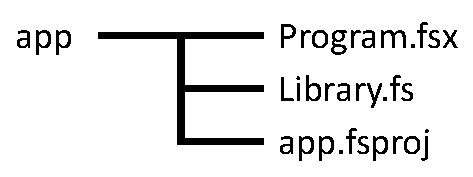
\includegraphics[width=0.35\linewidth]{dotnetLightNew}
  \caption{A set of files for a light version of a dotnet project.}
  \label{fig:dotnetNewLightFileSystem}
\end{figure}
 The \lstinline[language=console]{.fsproj} file is an XML-file which describes how dotnet should combine various files. The \lstinline[language=console]{dotnet} command-line tool can edit this file, but we might as well do this ourselves in a text editor: Open the file in your favorite text editor and in the \lstinline[language=console]{<ItemGroup>} change \lstinline[language=console]{Program.fs} to \lstinline[language=console]{Program.fsx} and add a line with the name of your library file \lstinline[language=console]{<Compile Include="Library.fs" />}. The resulting file should look like this:
\begin{codeNOutput}[label=appLightFsproj,
  top=-5pt,
  bottom=-5pt,
  left=-2pt,
  right=-2pt,
]{: The initial content of \texttt{app.fsproj}.}
  \begin{lstlisting}[language=console,escapechar=§]
<Project Sdk="Microsoft.NET.Sdk">
 <PropertyGroup>
  <OutputType>Exe</OutputType>
  <TargetFramework>net6.0</TargetFramework>
 </PropertyGroup>
 <ItemGroup>
  <Compile Include="Library.fs" />
  <Compile Include="Program.fsx" />
 </ItemGroup>
</Project>
\end{lstlisting}
\end{codeNOutput}
If you decide to rename the application or library files, then you must update the project files accordingly.

If you wish to add references to packages such as the \lstinline{DIKU.Canvas} package, this can be done as,
\begin{codeNOutput}[label=dotnetNew,
  top=-5pt,
  bottom=-5pt,
  left=-2pt,
  right=-2pt,
]{: Creating an initial library-application file setup.}
  \begin{lstlisting}[language=console,escapechar=§]
$ dotnet add app/app.fsproj package "DIKU.Canvas" --version 1.0.1
\end{lstlisting}%$
\end{codeNOutput}
or manually by editing the project file appropriately. When a package is included in the project file, then it does not need to be loaded in libraries and applications using the \lstinline{#r} directive. This version will compile and run the library and the program, but will not build the library separately.

The order of the references to packages, libraries, and application files are important, since \lstinline[language=console]{dotnet} will read them from top to bottom, and only if, e.g., \lstinline[language=console]{Library.fs} is above \lstinline[language=console]{Program.fsx} will the library functions be available in the application.

As an example, change \lstinline[language=console]{Program.fs} to become what is shown in \Cref{program},
\fsImplementation{solution/app/Program}{program}{A simple application program.}{}
change \lstinline[language=console]{Library.fs} to become what is shown in \Cref{library}, 
\fsImplementation{solution/library/Library}{library}{A simple library.}{}
and run it in \idx{compile mode} by changing to the \lstinline[language=console]{app} directory and using the \lstinline[language=console]{dotnet run} command as demonstrated in \Cref{dotnetRun}.
\begin{codeNOutput}[label=dotnetRun,
  top=-5pt,
  bottom=-5pt,
  left=-2pt,
  right=-2pt,
]{: Running an application setup with one or more project files.}
  \begin{lstlisting}[language=console,escapechar=§]
$ cd solution/app
$ dotnet run
"Greetings Jon"
\end{lstlisting}%$
\end{codeNOutput}
Assuming that \lstinline[language=console]{Program.fs} was renamed to \lstinline[language=console]{Program.fsx} and \lstinline[language=console]{app.fsproj} was edited appropriately, \lstinline[language=console]{dotnet run} is almost the same as
\begin{codeNOutput}[label=dotnetRun,
  top=-5pt,
  bottom=-5pt,
  left=-2pt,
  right=-2pt,
]{: Running an application setup with one or more project files.}
  \begin{lstlisting}[language=console,escapechar=§]
$ dotnet fsi ../library/Library.fs Program.fsx
"Greetings Jon"
\end{lstlisting}%$
\end{codeNOutput}
However, \lstinline[language=console]{dotnet fsi} \idx{interprets} the library and application into executable code everytime it is called, while \lstinline[language=console]{dotnet run} only \idx{compiles} the program once. On my laptop, the time these different steps take depends on what else is running on the computer, but typical timings are
\begin{center}
  \rowcolors{2}{oddRowColor}{evenRowColor}
  \begin{tabular}{|l|l|}
    \hline
    \rowcolor{headerRowColor} Command & Time\\
    \hline
    \lstinline[language=console]|dotnet fsi ../library/Library.fs Program.fsx| & 1.2s\\
    \lstinline[language=console]|dotnet run| (first time) & 4.0s\\
    \lstinline[language=console]|dotnet run| & 1.0s\\
    \hline
\end{tabular}
\end{center}
The example application, we are studying here, is tiny, but even in this case, the repeated translation by \lstinline[language=console]{dotnet fsi} is a 16\% overhead when compared to an already compiled program, and you should expect this overhead to be larger for larger programs. However, for tiny programs, the cost of the initial compilation is 400\% and not worth the effort from a time perspective.


\section{Libraries and applications}
\label{sec:modules}
A library in F\# is expressed as a \idx{module}, which is a programming structure used to organize type declarations, values, functions, etc. The libraries should have the suffix \lstinline[language=console]{.fs}, and here will call them \idx{implementation files} in contrast to the signature files to be discussed below, which we will call \idx{signature files}.

A module is typically a file where the module name is declared in the first lines using the \idx[module@\lstinline{module}]{\keyword{module}} with the following syntax,
%
\begin{verbatimwrite}{\ebnf/outerModule.ebnf}
module <*ident*>
<*script*>
\end{verbatimwrite}
\syntax{\ebnf/outerModule.ebnf}{Outer module.}
%
Here, the identifier \lstinline[language=syntax]{<*ident*>} is a name not necessarily related to the filename, and the script \lstinline[language=syntax]{<*script*>} is an expression.

Consider the example from \Cref{solveQuadraticEquation} in which functions are defined for solving the values of $x$ where $f(x)=0$ for a quadratic equation. In the following, we will split this into a library of functions and an application program. For this, we set up a project system of files as described in \Cref{chap:projects}, where \lstinline[language=console]{Program.fs} has been replaced by \lstinline[language=console]{Program.fsx} and the \lstinline[language=console]{app.fsproj} has been edited appropriately. The content of  \lstinline[language=console]{Library.fs} has been changed to become what is shown in \Cref{quadraticModule}, 
\fsImplementation{solve/library/Library}{quadraticModule}{A library for solving quadratic equations.}{}
and \lstinline[language=console]{Program.fsx} has been changed to what is shown in \Cref{quadraticApp}.
\fsCode{solve/app/Program}{quadraticApp}{An application using the \lstinline!Solve! module.}{}

\section{Specifying a Module's Interface with a Signature File}
As the 8-step guide suggests, the design of programs is helped by first considering what the program's function is to do before actually implementing them. This also holds for libraries, and signature files can aid this process. 

A \idx[signature file]{signature files} is a file accompanying \idx{implementation files} and have the suffix \lstinline[language=console]{.fsi}. A signature file contains almost no implementation, but only type definitions. Signature files offer three distinct features:
\begin{enumerate}
\item Signature files can be used as part of the documentation of code since type information is of paramount importance for an application programmer to use a library. 
\item Signature files may be written before the implementation file. This allows for a higher-level programming design that focuses on \emph{which} functions should be included and \emph{how} they can be composed.
\item Signature files allow for access control. Most importantly, if a type definition is not available in the signature file, then it is not available to the application program. Such definitions are private and can only be used internally in the library code. More fine-grained control related to classes is available and will be discussed in \Cref{chap:oop}.
\end{enumerate}
These features help the programmer structure the process of programming and protect the user of a library from irrelevant data and functions. A signature file contains the type definitions and the types of values and functions to be exposed to the user of the library. For example, for the library in \Cref{quadraticModule}, we can define a signature files which makes the \lstinline{solveQuadraticEquation} function but not the \lstinline{discriminant} function available to the user of the library as demonstrated in \Cref{librarySignature}.
\fsSignature{solve/library/Library}{librarySignature}{A signature file for \Cref{quadraticModule}.}{}
To compile the application using the signature file, we must add the created file, e.g., \lstinline[language=console]{Library.fsi}, to the project file as, e.g., shown in \Cref{libraryFsprojFSI}.
\begin{codeNOutput}[label=libraryFsprojFSI,
  top=-5pt,
  bottom=-5pt,
  left=-2pt,
  right=-2pt,
]{: The \texttt{library.fsproj} with a signature file added.}
  \begin{lstlisting}[language=console,escapechar=§]
<Project Sdk="Microsoft.NET.Sdk">
 <PropertyGroup>
  <OutputType>Exe</OutputType>
  <TargetFramework>net6.0</TargetFramework>
 </PropertyGroup>
 <ItemGroup>
  <PackageReference Include="DIKU.Canvas" Version="1.0.1" />
  <Compile Include="Library.fsi" />
  <Compile Include="Library.fs" />
  <Compile Include="Program.fsx" />
 </ItemGroup>
</Project>
\end{lstlisting}
\end{codeNOutput}
In the context of the 8-step guide, it is useful to write the signature file before the implementation file, and that the signature file contains the documentation for the functions available in the application.

For technical reasons in the  \lstinline[language=console]{dotnet} framework, exposed type abbreviations must be given both in the signature file and the implementation file. The implication is that the signature at times must also define implementation details, see e.g., the example below, and thus becomes less abstract the desirable in general.

\section{Programming Intermezzo: Postfix Arithmetic with a Stack}
To this point, we have performed simple arithmetic using \idx{infix} notation, meaning that expressions like $(4+6*3)/2-8$ are evaluated using the precedence and association rules of the operators as
\begin{align}
  (4+6*3)/2-8
  &\rightsquigarrow (4+18)/2-8\\
  &\rightsquigarrow 22/2-8\\
  &\rightsquigarrow 11-8\\
  &\rightsquigarrow 3
\end{align}
However, there is an equally valid notation, \idx{postfix}, in which the same expression is written as $4\; 6\; 3\; *\; +\; 2\; /\; 8\; -$. Here, the rule is to read from left to right, and whenever there are two values and an operator, $a\; b\; \text{op}$, replaced this with the value $a \text{ op } b$ and repeat until only one value remains, which is the result of the calculation. Hence,
\begin{align}
  4\; 6\; 3\; *\; +\; 2\; /\; 8\; -
  &\rightsquigarrow\; 4\; 18\; +\; 2\; /\; 8\; -\\
  &\rightsquigarrow\; 22\; 2\; /\; 8\; -\\
  &\rightsquigarrow\; 11\; 8\; -\\
  &\rightsquigarrow\; 3
\end{align}
This was implemented on a series of calculators released by Hewlett-Packard in the 1960-1980'ies, and one of the arguments for this notation was, that the expressions could be evaluated by a stack with only 3 levels. In the following, we will look at stacks as an abstract datatype and build a library for stacks and an arithmetic solver for such simple expressions using this stack.

A stack is an abstract datatype, meaning that it is defined by its concepts, not its implementation. The concept of a stack is like a stack of plates in a cafeteria, they are placed in a physical stack, and you can take the top plate and place a plate on the top, but you cannot access a plate in the middle of a stack. Stacks typically come with the following functions:
\begin{description}
\item[init:] Create an empty stack.
\item[pop:] Return the top element and the resulting stack.
\item[push:] Put an element on a stack and return the resulting stack.
\item[isEmpty:] Check whether the stack is empty.
\end{description}
Following the 8-step guide \Cref{sec:8step}, the above directly suggests names and includes brief descriptions (Steps 1 and 2). Step 3 suggests that we write a simple test, and
since we are fond of piping, our test program is shown in \Cref{postfixTest}.
\fsCode{postfixTest}{postfixTest}{A simple program using a yet to be written library.}{}
We expect this to print the result of the last \lstinline{pop} call, which should include information about the element \lstinline{2}.

In the functional programming paradigm, our stack is a constant, implying that every time we pop and push, we create new stacks. Thus, for step 4 in the 8-step guide, we must accept that all but \lstinline{isEmpty} returns a new stack, and all but \lstinline{init} must take a stack as input. Thus we arrive at a signature file for the stack-library given in \Cref{librarySignature}.
\fsSignature{postfixLibrary}{librarySignature}{A signature file for the stack library}{} 
A limitation to F\#'s modules is that the type specifications need explicit declaration. We would have liked to write \lstinline{type stack} and functions of some variable type \lstinline{'e}, since the stack concept is independent of the type of elements it contains. However, this is not possible, and thus, we here specialize to integer stacks. For similar reasons, we are forced to specify details about the implementation of our type. Our idea is that stacks can be implemented as lists since lists are well suited to work with the first elements.

Implementing a stack using lists is simple, since lists already contains the properties \lstinline{Head}, \lstinline{Tail}, and \lstinline{IsEmpty}, which closely mimics the needed operations for a stack. Thus we arrive at \Cref{postfixImplementation}.
\fsImplementation{postfixLibrary}{postfixImplementation}{An implementation of a stack module.}{}
And now we can run our test code as shown in \Cref{postfixTestRun}.
\fsOutput{postfixTest}{postfixTestRun}{Running the test program}{}
As expected, the top element and the resulting stack is \lstinline{(2,[1])}.

To implement simple postfix algebra, we will use discriminated unions. That is, we define a type,
\begin{quote}
\lstinline{type element = Value of int | Multiply | Plus | Minus | Divide}
\end{quote}
This allows us to make lists of tokens such as,
\begin{quote}
\lstinline{[Value 4; Value 6; Value 3; Multiply; Plus]}
\end{quote}
for the expression $3\; 4\; 2\; /\; +$ which is equivalent to $3+4/2$ in infix notation. The next step is to understand how to use a stack to evaluate such expressions. The idea is to process the list of tokens from its head and push values to a stack. When the head of the tokens list is an operator, say 'op' then the two top elements from the stack are popped, say $a$ and $b$, the mathematical expression $c = a\text{ op }b$ is evaluated and $c$ is pushed to the stack. For our example, the evolution of the stack will be:
\begin{center}
  \begin{tabular}{l|r}
  Unused tokens &  Evaluation stack\\\hline
  $4\; 6\; 3\; *\; +\; 2\; /\; 8\; -$ & \lstinline![]! \\
  $6\; 3\; *\; +\; 2\; /\; 8\; -$ & \lstinline![4]! \\
  $3\; *\; +\; 2\; /\; 8\; -$ & \lstinline![6; 4]! \\
  $*\; +\; 2\; /\; 8\; -$ & \lstinline![3; 6; 4]! \\
  $+\; 2\; /\; 8\; -$ & \lstinline![18; 4]! \\
  $2\; /\; 8\; -$ & \lstinline![22]! \\
  $/\; 8\; -$ & \lstinline![2; 22]! \\
  $8\; -$ & \lstinline![11]! \\
  $-$ & \lstinline![8; 11]! \\
   & \lstinline![3]! \\
\end{tabular}
\end{center}
As demonstrated, the result of the expression is the last element on the stack, once the list of tokens is empty. An F\# implementaiton is given in \Cref{postfixApp}.
\fs{postfixApp}{An application for evaluating lists of tokens on postfix form using a stack.}

\section{Generic Modules}
\label{sec:genericModule}
The stack is an example of an abstract datatype, and in the previous section, we implemented a stack for integers, however, stacks can be of many other types, and although we could make a stack module for each type, it would greatly improve the usefulness of our library, if we could make a stack module, which is generic, i.e., where the user can decide when writing applications, which type of values to stack. Luckily, this is supported in F\#.

In \Cref{sec:variableType} we discussed the usefulness of the variable type such as \lstinline{'a}, which makes functions and types generic, that is, the same definition can be used for any type. To make a generic module, it is often useful first to make a non-generic version, such as our integer stack, since it is often easier to spot errors in concrete program versions. The integer stack already works as desired, so we will now modify the module to be a stack for a variable type. In our example, we must update both the type abbreviation and function types in the signature file. The result is shown in \Cref{postfixLibraryGeneric}.
\fsSignature{postfixLibraryGeneric}{librarySignature}{A signature file for the generic stack library}{} 
The next step is to update the implementation file. During such transformations, it is not uncommon to realize that restrictions must be put on the type, which is possible but which we will not consider further in this book. Since the stack does not rely on any properties of the stack elements, there is no challenge in modifying the implementation file as shown in \Cref{postfixLibraryGeneric}.
\fsImplementation{postfixLibraryGeneric}{postfixImplementation}{An implementation of a generic stack module.}{}
Finally, we can make an application using stacks of various kinds, as shown in \Cref{postfixTestGeneric}.
\fs{postfixTestGeneric}{Running the test program}{}
In the program, we see that F\# can infer that a stack, on which integers are pushed, must be of \lstinline{stack<int>} type, and when characters are pushed, then the stack must be of type \lstinline{stack<char>}. Thus, we have arrived at a stack for any type, whose interface is given by the signature file, and almost all of its implementation is hidden in the implementation file.

\section{Key Concepts and Terms in This Chapter}
In this chapter, we have looked at how to build libraries and applications. Key concepts have been
\begin{itemize}
\item How to build organise the compilation of libraries and applications using \lstinline[language=console]{dotnet} \textbf{project files}.
\item How to design libraries using \textbf{modules} and \textbf{signature files}.
\item How to make \textbf{library implementation files}.
\item How to implement the \textbf{abstract datatype Stack} both as an integer stack and as a \textbf{generic module}. 
\end{itemize}

\end{document}



\chapter{Object-oriented programming}
\label{chap:oop}
Things to remember: 
\begin{itemize}
\item upcast and downcast \keyword{upcast}, \token{:>},
  \keyword{downcast}, \token{:?>}
\item boxing \lstinline|(box 5) :?> int;;|, see Spec-4.0 chapter
  18.2.6.
\item obj type Spec-4.0 chapter 18.1
\end{itemize}
%%% Local Variables:
%%% TeX-master: "fsharpNotes"
%%% End:


\documentclass[springer.tex]{subfiles}
\graphicspath{ {./figures/} }

\begin{document}
\part{Appendix}
\label{part:appendix}
\appendix
\end{document}
%%% Local Variables:
%%% TeX-master: "fsharpNotes"
%%% End:


\chapter{Number systems on the computer}
\section{Binary numbers}
\label{sec:binary}
Humans like to use the \idx{decimal number} system for representing numbers. Decimal numbers are \idx{base} 10 means that for a number consisting of a sequence of digits separated by a \idx{decimal point}, where each \idx{digit} can have values $d \in \{0,1,2,\ldots,9\}$ and the weight of each digit is proportional to its place in the sequence of digits w.r.t.\ the decimal point, i.e., the number $357.6=3\cdot 10^2+5\cdot 10^1+7\cdot 10^0+6\cdot 10^{-1}$ or in general:
\begin{align}
  v = \sum_{i=-m}^nd_i10^i
\end{align}
The basic unit of information in almost all computers is the binary digit or \idx{bit} for short. A \idx{binary} number consists of a sequence of binary digits separated by a decimal point, where each digit can have values $b \in \{0,1\}$, and the base is $2$. The general equation is,
\begin{align}
  v = \sum_{i=-m}^nb_i2^i
\end{align}
and examples are $1011.1_2 = 1\cdot 2^3+0\cdot 2^2+1\cdot 2^1+1\cdot 2^0+1\cdot 2^{-1} = 11.5$. Notice that we use subscript 2 to denote a binary number, while no subscript is used for decimal numbers. Due to typical organization of computer memory, 8 binary digits is called a \idx{byte}, and 32 digits a \idx{word}.

Other number systems are often used, e.g., \idx{octal} numbers, which are base 8 numbers, where each digit is $o\in\{0,1,\ldots,7\}$. Octals are useful short-hand for binary, since 3 binary digits maps to the set of octal digits. Likewise, \idx{hexadecimal} numbers are base 16 with digits $h\in\{0,1,2,3,4,5,6,7,8,9,a,b,c,d,e,f\}$, such that $a_{16}=10$, $b_{16}=11$ and so on. Hexadecimals are convenient since 4 binary digits map directly to the set of octal digits. Thus $367 = 101101111_2 = 557_8 = 16f_{16}$. A list of the intergers 0--63 is various bases is given in Table~\ref{tab:binaryTable}.
\begin{table}
  \centering
  \begin{tabular}{|r|r|r|r|}
    \hline
    Dec & Bin & Oct & Hex\\
    \hline
    0 & 0 & 0 & 0\\
    1 & 1 & 1 & 1\\
    2 & 10 & 2 & 2\\
    3 & 11 & 3 & 3 \\
    4 & 100 & 4 & 4\\
    5 & 101 & 5& 5\\
    6 & 110 & 6 & 6 \\
    7 & 111 & 7 & 7 \\
    8 & 1000 & 10 & 8\\
    9 & 1001 & 11 & 9\\
    10 & 1010 & 12 & a\\
    11 & 1011 & 13 & b\\
    12 & 1100 & 14 & c\\
    13 & 1101 & 15 & d\\
    14 & 1110 & 16 & e \\
    15 & 1111 & 17 & f\\
    16 & 10000 & 20 & 10\\
    17 & 10001 & 21 & 11\\
    18 & 10010 & 22 & 12\\
    19 & 10011 & 23 & 13 \\
    20 & 10100 & 24 & 14\\
    21 & 10101 & 25& 15\\
    22 & 10110 & 26 & 16 \\
    23 & 10111 & 27 & 17 \\
    24 & 11000 & 30 & 18\\
    25 & 11001 & 31 & 19\\
    26 & 11010 & 32 & 1a\\
    27 & 11011 & 33 & 1b\\
    28 & 11100 & 34 & 1c\\
    29 & 11101 & 35 & 1d\\
    30 & 11110 & 36 & 1e \\
    31 & 11111 & 37 & 1f\\
    \hline
  \end{tabular}
  \begin{tabular}{|r|r|r|r|}
    \hline
    Dec & Bin & Oct & Hex\\
    \hline
    32 & 100000 & 40 & 20\\
    33 & 100001 & 41 & 21\\
    34 & 100010 & 42 & 22\\
    35 & 100011 & 43 & 23 \\
    36 & 100100 & 44 & 24\\
    37 & 100101 & 45& 25\\
    38 & 100110 & 46 & 26 \\
    39 & 100111 & 47 & 27 \\
    40 & 101000 & 50 & 28\\
    41 & 101001 & 51 & 29\\
    42 & 101010 & 52 & 2a\\
    43 & 101011 & 53 & 2b\\
    44 & 101100 & 54 & 2c\\
    45 & 101101 & 55 & 2d\\
    46 & 101110 & 56 & 2e \\
    47 & 101111 & 57 & 2f\\
    48 & 110000 & 60 & 30\\
    49 & 110001 & 61 & 31\\
    50 & 110010 & 62 & 32\\
    51 & 110011 & 63 & 33 \\
    52 & 110100 & 64 & 34\\
    53 & 110101 & 65 & 35\\
    54 & 110110 & 66 & 36 \\
    55 & 110111 & 67 & 37 \\
    56 & 111000 & 70 & 38\\
    57 & 111001 & 71 & 39\\
    58 & 111010 & 72 & 3a\\
    59 & 111011 & 73 & 3b\\
    60 & 111100 & 74 & 3c\\
    61 & 111101 & 75 & 3d\\
    62 & 111110 & 76 & 3e \\
    63 & 111111 & 77 & 3f\\
    \hline
  \end{tabular}
  \caption{A list of the intergers 0--63 in decimal, binary, octal, and hexadecimal.}
  \label{tab:binaryTable}
\end{table}
\section{IEEE 754 floating point standard}
\label{sec:floatingPoint}
The set of real numbers also called \idx{reals} includes all fractions and irrational numbers. It is infinite in size both in the sense that there is no largest nor smallest number and between any 2 given numbers there are infinitely many numbers. Reals are widely used for calculation, but since any computer only has finite memory, it is impossible to represent all possible reals. Hence, any computation performed on a computer with reals must rely on approximations. \idx{IEEE 754 double precision floating-point format} (\idx{binary64}), known as a \idx{double}, is a standard for representing an approximation of reals using 64 bits. These bits are divided into 3 parts: sign, exponent and fraction, 
\begin{displaymath}
  s\, e_1 e_2 \ldots e_{11}\, m_1 m_2 \ldots m_{52},
\end{displaymath}
where $s$, $e_i$, and $m_j$ are binary digits. The bits are converted to a number using the equation by first calculating the exponent $e$ and the mantissa $m$,
\begin{align}
  e &= \sum _{i=1}^{11}e_i2^{11-i},\\
  m & = \sum _{j=1}^{52}m_j2^{-j}.
\end{align}
I.e., the exponent is an integer, where $0 \leq e < 2^{11}$, and the mantissa is a rational, where $0 \leq m < 1$. For most combinations of $e$ and $m$ the real number $v$ is calculated as,
\begin{equation}
  v = \left(-1\right)^{s} \left(1+m\right) 2^{e-1023}
\end{equation}
 with the exception that
\begin{center}
  \begin{tabular}{|l|l|l|}
    \hline
                         & $m=0$                                   & $m\neq 0$\\
    \hline
    $e=0$           & $v = \left(-1\right)^{s} 0$ (signed zero) & $v = \left(-1\right)^{s} m 2^{1-1023}$ (subnormals)\\
    \hline 
    $e=2^{11}-1$ & $v = \left(-1\right)^{s} \infty$               & $v = \left(-1\right)^{s} \text{NaN}$ (not a number)\\
    \hline
  \end{tabular}
\idxs{subnormals}\idxs{NaN}\idxs{not a number}
\end{center}
where $e=2^{11}-1=11111111111_2=2047$. The largest and smallest number that is not infinity is thus
\begin{align}
  e &= 2^{11}-2 = 2046\\
  m &= \sum _{j=1}^{52}2^{-j} = 1 - 2^{-52} \simeq 1.\\
  v_\text{max} &= \pm \left(2-2^{-52}\right) 2^{1023} \simeq \pm 2^{1024} \simeq \pm 10^{308}
\end{align}
The density of numbers varies in such a way that when $e-1023 = 52$, then
\begin{align}
  v &= \left(-1\right)^{s} \left(1+\sum _{j=1}^{52}m_j2^{-j}\right) 2^{52} 
  \\&= \pm \left(2^{52}+\sum _{j=1}^{52}m_j2^{-j}2^{52}\right) 
  \\&= \pm \left(2^{52}+\sum _{j=1}^{52}m_j2^{52-j}\right) 
  \\&\overset{k=52-j}{=} \pm \left(2^{52}+\sum _{k=51}^{0}m_{52-k}2^k\right) 
\end{align}
which are all integers in the range $2^{52}\leq |v| < 2^{53}$. When $e-1023 = 53$, then the same calculation gives
\begin{align}
  v &\overset{k=53-j}{=} \pm \left(2^{53}+\sum _{k=52}^{1}m_{53-k}2^k\right) 
\end{align}
which are every second integer in the range $2^{53}\leq |v| < 2^{54}$, and so on for larger $e$. When $e-1023 = 51$, then the same calculation gives,
\begin{align}
  v &\overset{k=51-j}{=} \pm \left(2^{51}+\sum _{k=50}^{-1}m_{51-k}2^k\right) 
\end{align}
which gives a distance between numbers of $1/2$ in the range $2^{51}\leq |v| < 2^{52}$, and so on for smaller $e$. Thus we may conclude that the distance between numbers in the interval $2^n\leq |v| < 2^{n+1}$ is $2^{n-52}$, for $-1022 = 1-1023\leq n<2046-1023=1023$.  For subnormals the distance between numbers are
\begin{align}
  v &= \left(-1\right)^{s} \left(\sum _{j=1}^{52}m_j2^{-j}\right) 2^{-1022} 
  \\&= \pm \left(\sum _{j=1}^{52}m_j2^{-j}2^{-1022}\right) 
  \\&= \pm \left(\sum _{j=1}^{52}m_j2^{-j -1022}\right) 
  \\&\overset{k=-j-1022}{=} \pm \left(\sum _{j=-1023}^{-1074}m_{-k-1022}2^k\right) 
\end{align}
which gives a distance between numbers of $2^{-1074} \simeq 10^{-323}$ in the range $0<|v|<2^{-1022}\simeq10^{-308}$.

%%% Local Variables:
%%% TeX-master: "fsharpNotes"
%%% End:


\documentclass[springer.tex]{subfiles}
\graphicspath{ {./figures/} }

\begin{document}
\chapter{Commonly Used Character Sets}
\label{sec:characterSets}
Letters, digits, symbols, and space are the core of how we store data, write programs, and communicate with computers and each other. These symbols are in short called characters and represent a mapping between numbers, also known as codes, and a pictorial representation of the character. E.g., the ASCII code for the letter 'A' is 65. These mappings are for short called character sets, and due to differences in natural languages and symbols used across the globe, many different character sets are in use. E.g., the English alphabet contains the letters 'a' to 'z'. These letters are common to many other European languages which in addition use even more symbols and accents. For example, Danish has further the letters 'æ', 'ø', and 'å'. Many non-European languages have completely different symbols, where the Chinese character set is probably the most extreme, and some definitions contain 106,230 different characters, albeit only 2,600 are included in the official Chinese language test at the highest level.

Presently, the most common character set used is Unicode Transformation Format (UTF), whose most popular encoding schemes are 8-bit (UTF-8) and 16-bit (UTF-16). Many other character sets exist, and many of the later build on the American Standard Code for Information Interchange (ASCII). The ISO-8859 codes were an intermediate set of character sets that are still in use, but which is greatly inferior to UTF. Here we will briefly give an overview of ASCII, ISO-8859-1 (Latin1), and UTF.

\section{ASCII}
\label{sec:ascii}
The \idx{American Standard Code for Information Interchange} (\idx{ASCII})~\cite{ascii63}, is a 7 bit code tuned for the letters of the English language, numbers, punctuation symbols, control codes and space, see \Cref{tab:ascii,tab:asciiSpecialSymbols}.
\begin{table}
  \centering
  \rowcolors{2}{oddRowColor}{evenRowColor}
  \begin{tabularx}{0.95\textwidth}{|*{17}{>{\centering\arraybackslash}X|}}
    \hline
    \rowcolor{headerRowColor} x0+0x & 00 & 10 & 20 & 30 & 40 & 50 & 60 & 70 \\
    \hline
    00 & NUL & DLE & SP & 0 & @ & P & ` & p \\
    \hline
    01 & SOH & DC1 & ! & 1 & A & Q & a & q \\
    \hline
    02 & STX & DC2 & " & 2 & B & R & b & r \\
    \hline
    03 & ETX & DC3 & \# & 3 & C & S & c & s \\
    \hline
    04 & EOT & DC4 & \$ & 4 & D & T & d & t \\
    \hline
    05 & ENQ & NAK & \% & 5 & E & U & e & u \\
    \hline
    06 & ACK & SYN & \& & 6 & F & V & f & v \\
    \hline
    07 & BEL & ETB & ' & 7 & G & W & g & w \\
    \hline
    08 & BS & CAN & ( & 8 & H & X & h & x \\
    \hline
    09 & HT & EM & ) & 9 & I & Y & i & y \\
    \hline
    0A & LF & SUB & * & : & J & Z & j & z \\
    \hline
    0B & VT & ESC & + & ; & K & [ & k & $\{$\\
    \hline
    0C & FF & FS & , & $<$ & L & \textbackslash & l & $|$\\
    \hline
    0D & CR & GS & $-$ & = & M & ] & m & $\}$\\
    \hline
    0E & SO & RS & . & $>$ & N & \textasciicircum & n & \textasciitilde\\
    \hline
    0F & SI & US & / & ? & O & \_ & o & DEL\\
    \hline
  \end{tabularx}
  \caption{ASCII}
  \label{tab:ascii}
\end{table}
\begin{table}
  \centering
  \rowcolors{2}{oddRowColor}{evenRowColor}
  \begin{tabular}{|l|l|}
    \hline
    \rowcolor{headerRowColor} Code & Description\\
    \hline
    NUL & Null\\
    SOH & Start of heading\\
    STX & Start of text\\
    ETX & End of text\\
    EOT & End of transmission\\
    ENQ & Enquiry\\
    ACK & Acknowledge\\
    BEL & Bell\\
    BS & Backspace\\
    HT & Horizontal tabulation\\
    LF & Line feed\\
    VT & Vertical tabulation\\
    FF & Form feed\\
    CR & Carriage return\\
    SO & Shift out\\
    SI & Shift in\\
    DLE & Data link escape\\
    DC1 & Device control one\\
    DC2 & Device control two\\
    DC3 & Device control three\\
    DC4 & Device control four\\
    NAK & Negative acknowledge\\
    SYN & Synchronous idle\\
    ETB & End of transmission block\\
    CAN & Cancel\\
    EM & End of medium\\
    SUB & Substitute\\
    ESC & Escape\\
    FS & File separator\\
    GS & Group separator\\
    RS & Record separator\\
    US & Unit separator\\
    SP & Space\\
    DEL & Delete\\
    \hline
  \end{tabular}
  \caption{ASCII symbols.}
  \label{tab:asciiSpecialSymbols}
\end{table}
The first 32 codes are reserved for non-printable control characters to control printers and similar devices or to provide meta-information. The meaning of each control character is not universally agreed upon.

The code order is known as \idx{ASCIIbetical order}, and it is sometimes used to perform arithmetic on codes, e.g., an uppercase letter with code $c$ may be converted to lower case by adding 32 to its code. The ASCIIbetical order also has a consequence for sorting, i.e., when sorting characters according to their ASCII code, 'A' comes before 'a', which comes before the symbol '$\{$'.

\section{ISO/IEC 8859}
The ISO/IEC 8859 report \url{http://www.iso.org/iso/catalogue_detail?csnumber=28245} defines 10 sets of codes specifying up to 191 codes and graphics characters using 8 bits. Set 1, also known as ISO/IEC 8859-1, Latin alphabet No.\ 1, or \idx{Latin1}, covers many European languages and is designed to be compatible with ASCII, such that code for the printable characters in ASCII is the same in ISO 8859-1. \Cref{tab:latin1} shows the characters above 7e. Codes 00-1f and 7f-9f are undefined in ISO 8859-1. 
\begin{table}
  \centering
  \rowcolors{2}{oddRowColor}{evenRowColor}
  \begin{tabularx}{0.95\textwidth}{|*{17}{>{\centering\arraybackslash}X|}}
    \hline
    \rowcolor{headerRowColor} x0+0x & 80 & 90 & A0 & B0 & C0 & D0 & E0 & F0 \\
    \hline
    00 & & & NBSP & $^\circ$ & \`A & \DH & \`a &\dh\\
    \hline
    01 & & & \textexclamdown & $\pm$ & \'A & \~N & \'a &\~n\\
    \hline
    02 & & & \textcent & $^2$ & \^A & \`O & \^a &\`o\\
    \hline
    03 & & & \pounds & $^3$ & \~A & \'O & \~a &\'o\\
    \hline
    04 & & & \textcurrency & \'{} & \"A & \^O & \"a &\^o\\
    \hline
    05 & & & \textyen & $\mu$ & \r A & \~O & \r a &\~o\\
    \hline
    06 & & & \textbrokenbar & \P & \AE & \"O & \ae &\"o\\
    \hline
    07 & & & \S & \textperiodcentered & \c C & $\times$ & \c c &$\div$\\
    \hline
    08 & & & \"{} & \c\ & \`E & \O & \`e &\o\\
    \hline
    09 & & & \copyright & $^1$ & \'E & \`U & \'e &\`u\\
    \hline
    0a & & & \textordfeminine & \textordmasculine & \^E & \'U & \^e &\'u\\
    \hline
    0b & & & \guillemotleft & \guillemotright & \"E & \^U & \"e &\^u\\
    \hline
    0c & & & $\lnot$ & $\frac14$ & \`I & \"U & \`\i &\"u\\
    \hline
    0d & & & SHY & $\frac12$ & \'I & \'Y & \'\i &\'y\\
    \hline
    0e & & & \textregistered & $\frac34$ & \^I & \TH & \^\i &\th\\
    \hline
    0f & & & \={} & \textquestiondown & \"I & \ss & \"\i &\"y\\
    \hline
  \end{tabularx}
  \caption{ISO-8859-1 (latin1) non-ASCII part. Note that the codes 7f -- 9f are undefined.}
  \label{tab:latin1}
\end{table}
\begin{table}
  \centering
  \rowcolors{2}{oddRowColor}{evenRowColor}
  \begin{tabular}{|l|l|}
    \hline
    \rowcolor{headerRowColor} Code & Description\\
    \hline
    NBSP & Non-breakable space\\
    SHY & Soft hypen\\
    \hline
  \end{tabular}
  \caption{ISO-8859-1 special symbols.}
  \label{tab:latin1SpecialSymbols}
\end{table}

\section{Unicode}
\label{sec:unicode}
Unicode is a character standard defined by the Unicode Consortium, \url{http://unicode.org}, as the \idx{Unicode Standard}. Unicode allows for 1,114,112 different codes. Each code is called a \idx{code point} which represents an abstract character. Code points are divided into 17 planes, each with $2^{16}=65,536$ code points. Planes are further subdivided into named \idx[unicode block]{blocks}. The first plane is called the \idx{Basic Multilingual plane} and its block of the first 128 code points is called the \idx{Basic Latin block} and is identical to ASCII, see \Cref{tab:ascii}, and code points 128-255 are called the \idx{Latin-1 Supplement block}, and are identical to the upper range of ISO 8859-1, see \Cref{tab:latin1}.  Each code-point has a number of attributes such as the \idx{Unicode general category}. Presently more than 128,000 code points are defined as covering 135 modern and historical writing systems, and obtained at \url{http://www.unicode.org/Public/UNIDATA/UnicodeData.txt}, which includes the code point, name, and general category.

A Unicode code point is an abstraction from the encoding and the graphical representation of a character. A code point is written as ``U+'' followed by its hexadecimal number, and for the Basic Multilingual plane, 4 digits are used, e.g., the code point with the unique name LATIN CAPITAL LETTER A has the Unicode code point ``U+0041'', and is in this text visualized as 'A'. More digits are used for code points of the remaining planes.

The general category is used to specify valid characters that do not necessarily have a visual representation but possibly transform text. Some categories and their letters in the first 256 code points are shown in \Cref{tab:generalCategories}.
\begin{table}
  \centering
%  \begin{tabularx}{0.75\linewidth}{|>{\hsize=1\hsize}X|\hsize=1\hsize}X|\hsize=1\hsize}X|}
  \rowcolors{2}{oddRowColor}{evenRowColor}
  \begin{tabularx}{\linewidth}{|>{\hsize=.3\hsize}X*{2}{|>{\hsize=1.35\hsize\raggedright\arraybackslash}X}|}    \hline
    \rowcolor{headerRowColor} General category & Code points & Name \\
    \hline
    Lu& U+0041--U+005A, U+00C0--U+00D6,  U+00D8--U+00DE & Upper case letter\\
    Ll& U+0061--U+007A, U+00B5, U+00DF--U+00F6, U+00F8--U+00FF & Lower case letter\\
    Lt& None & Digraphic letter, with first part uppercase \\
    Lm& None & Modifier letter \\
    Lo& U+00AA, U+00BA & Gender ordinal indicator \\
    Nl& None & Letterlike numeric character \\
    Pc& U+005F & Low line\\
    Mn&None & Nonspacing combining mark \\
    Mc&None & Spacing combining mark\\
    Cf& U+00AD & Soft Hyphen \\
    \hline
  \end{tabularx}
  \caption{Some general categories for the first 256 code points.}
  \label{tab:generalCategories}
\end{table}

To store and retrieve code points, they must be encoded and decoded. A common encoding is \idx{UTF-8}, which encodes code points as 1 to 4 bytes, and which is backward-compatible with ASCII and ISO 8859-1. Hence, in all 3 coding systems, the character with code 65 represents the character 'A'. Another popular encoding scheme is \idx{UTF-16}, which encodes characters as 2 or 4 bytes, but which is not backward-compatible with ASCII or ISO 8859-1. UTF-16 is used internally in many compilers, interpreters, and operating systems.
\end{document}


\documentclass[fsharpnotes.tex]{subfiles}

\begin{document}
\chapter{A brief introduction to Extended Backus-Naur Form}
\label{sec:ebnf}
\idx{Extended Backus-Naur Form} (\idx{EBNF}) is a language to specify programming languages in. The name is a tribute to John Backus who used it to describe the syntax of ALGOL58 and Peter Nauer for his work on ALGOL 60.

An EBNF consists of \idx{terminal symbols} and \idx{production rules}. Examples of typical terminal symbol are characters, numbers, punctuation marks, and whitespaces, e.g.,
\begin{lstlisting}[language=ebnf]
digit = "0" | "1" | "2" | "3" | "4" | "5" | "6" | "7" | "8" | "9";
\end{lstlisting}
A production rule specifies a method of combining other production rules and terminal symbols, e.g.,
\begin{lstlisting}[language=ebnf]
number = digit { digit };
\end{lstlisting}
A proposed standard for ebnf (proposal ISO/IEC 14977, \url{http://www.cl.cam.ac.uk/~mgk25/iso-14977.pdf}) is,
\begin{description}
\item '\lstinline[language=ebnf]|=|' definition, e.g., 
  \begin{lstlisting}[language=ebnf]
zero = "0";
  \end{lstlisting}
  here \lstinline[language=ebnf]|zero| is the terminal symbol \lstinline[language=ebnf]|0|.
\item '\lstinline[language=ebnf]|,|' concatenation, e.g.,
  \begin{lstlisting}[language=ebnf]
one = "1";
eleven = one, one;
  \end{lstlisting}
  here \lstinline[language=ebnf]|eleven| is the terminal symbol \lstinline[language=ebnf]|11|.
\item '\lstinline[language=ebnf]|;|' termination of line
\item '\lstinline[language=ebnf]!|!' alternative options, e.g.,
  \begin{lstlisting}[language=ebnf]
digit = "0" | "1" | "2" | "3" | "4" | "5" | "6" | "7" | "8" | "9";
  \end{lstlisting}
  here \lstinline[language=ebnf]|digit| is the single character terminal symbol, such as \lstinline[language=ebnf]|3|.
\item '\lstinline[language=ebnf]|[ ... ]|' optional, e.g.,
  \begin{lstlisting}[language=ebnf]
zero = "0";
nonZeroDigit = "1" | "2" | "3" | "4" | "5" | "6" | "7" | "8" | "9";
nonZero = [ zero ], nonZeroDigit;
  \end{lstlisting}
  here \lstinline[language=ebnf]|nonZero| is a non-zero digit possibly preceded by zero, such as \lstinline[language=ebnf]|02|.
\item '\lstinline[language=ebnf]|{ ... }|' repetition zero or more times, e.g., 
  \begin{lstlisting}[language=ebnf]
digit = "0" | "1" | "2" | "3" | "4" | "5" | "6" | "7" | "8" | "9";
number = digit, { digit };
  \end{lstlisting}
  here \lstinline[language=ebnf]|number| is a word consisting of 1 or more digits, such as \lstinline[language=ebnf]|12|.
\item '\lstinline[language=ebnf]|( ... )|' grouping, e.g.,
  \begin{lstlisting}[language=ebnf]
digit = "0" | "1" | "2" | "3" | "4" | "5" | "6" | "7" | "8" | "9";
signedNumber = ( "+" | "-" ) digit, { digit };
  \end{lstlisting}
  here \lstinline[language=ebnf]|signedNumber| is a number with a mandatory sign, such as \lstinline[language=ebnf]|+5| and \lstinline[language=ebnf]|-3|.
\item '\lstinline[language=ebnf]|" ... "|' a terminal string, e.g.,
  \begin{lstlisting}[language=ebnf]
string = "abc"';
  \end{lstlisting}
\item "\lstinline[language=ebnf]|' ... '|" a terminal string, e.g.,
  \begin{lstlisting}[language=ebnf]
string = 'abc';
  \end{lstlisting}
\item '\lstinline[language=ebnf]|(* ... *)|' a comment (* ... *) 
  \begin{lstlisting}[language=ebnf]
(* a binary digit *) digit = "0" | "1"; (* from this all numbers may be constructed *)
  \end{lstlisting}
  Everything inside the comments are not part of the formal definition.
\item '\lstinline[language=ebnf]|? ... ?|' special sequence, a notation reserved for future extensions of EBNF.
  \begin{lstlisting}[language=ebnf]
codepoint = ?Any unicode codepoint?;
  \end{lstlisting}
\item '\lstinline[language=ebnf]|-|' exception, e.g.,
  \begin{lstlisting}[language=ebnf]
letter = "A" | "B" | "C" | "D" | "E" | "F" | "G" | "H" 
  | "I" | "J" | "K" | "L" | "M" | "N" | "O" | "P" | "Q" 
  | "R" | "S" | "T" | "U" | "V" | "W" | "X" | "Y" | "Z";
vowel = "A" | "E" | "I" | "O" | "U"; 
consonant = letter - vowel;
  \end{lstlisting}
  here \lstinline[language=ebnf]|consonant| are all letters except vowels.
\end{description}

Rules for rewriting EBNF are:
\begin{center}
  \rowcolors{2}{oddRowColor}{evenRowColor}
  \begin{tabularx}{\linewidth}{|l|X|}
    \hline
    \rowcolor{headerRowColor} Rule & Description\\
    \hline
    \lstinline[language=ebnf]{s | t} $\leftrightarrow$ \lstinline[language=ebnf]{t | s} & \lstinline[language=ebnf]{|} is commutative \\
    \hline
    \lstinline[language=ebnf]{r | (s | t)} $\leftrightarrow$ \lstinline[language=ebnf]{(r | s) | t} $\leftrightarrow$ \lstinline[language=ebnf]{r | s | t} & \lstinline[language=ebnf]{|} is associative \\
    \hline
    \lstinline[language=ebnf]{(r, s) t} $\leftrightarrow$ \lstinline[language=ebnf]{r (s, t)} $\leftrightarrow$ \lstinline[language=ebnf]{r, s, t} & concatenation is associative \\
    \hline
    \lstinline[language=ebnf]{r, (s | t)} $\leftrightarrow$ \lstinline[language=ebnf]{r, t | r, s} & concatenation is distributive over \lstinline[language=ebnf]{|}\\
    \lstinline[language=ebnf]{(r | s), t} $\leftrightarrow$ \lstinline[language=ebnf]{r, t | r, t} &\\
    \hline
    \lstinline[language=ebnf]{[s | t]} $\leftrightarrow$ \lstinline[language=ebnf]{[t] | [s]} &\\
    \hline
    \lstinline[language=ebnf]{[[s]]} $\leftrightarrow$ \lstinline[language=ebnf]{[s]} & \lstinline[language=ebnf]{[]} is idempotent \\
    \hline
    \lstinline[language=ebnf]{\{\{s\}\}} $\leftrightarrow$ \lstinline[language=ebnf]{\{s\}} & \lstinline[language=ebnf]{\{\}} is idempotent \\
    \hline
  \end{tabularx}
\end{center}
where \lstinline[language=ebnf]{r}, \lstinline[language=ebnf]{s}, and \lstinline[language=ebnf]{t} are production rules or terminals. Precedence for the EBNF symbols are,
\begin{center}
  \rowcolors{2}{oddRowColor}{evenRowColor}
  \begin{tabular}{|l|l|}
    \hline
    \rowcolor{headerRowColor} Symbol & Description\\
    \hline
    \lstinline[language=ebnf]![]!, \ldots & Bracket and quotation mark pairs\\
    \hline
    \lstinline[language=ebnf]!-! & except\\
    \hline
    \lstinline[language=ebnf]!,! & concatenate\\
    \hline
    \lstinline[language=ebnf]!|! & option\\
    \hline
    \lstinline[language=ebnf]!=! & define\\
    \hline
    \lstinline[language=ebnf]!;! & terminator\\
    \hline
  \end{tabular}
\end{center}
in order of precedence, such that bracket and quotation mark pairs has higher precedence than \lstinline[language=ebnf]{-}. 
%These precedence rules are overridden by bracket pairs, such as \lstinline[language=ebnf]{' '}, \lstinline[language=ebnf]{" "}, \lstinline[language=ebnf]{(* *)}, \lstinline[language=ebnf]{( )}, \lstinline[language=ebnf]{[ ]}, \lstinline[language=ebnf]!{ }!, \lstinline{? ?}.

The proposal allows for identifies that includes space, but often a reduced form is used, where identifiers are single words, in which case the concatenation symbol \lstinline[language=ebnf]|,| is replaced by a space. Likewise, the termination symbol \lstinline[language=ebnf]|;| is often replaced with the new-line character, and if long lines must be broken, then indentation is used to signify continuation. In this relaxed EBNF, the EBNF syntax itself can be expressed in EBNF as,
\begin{lstlisting}[language=ebnf]
letter = "A" | "B" | "C" | "D" | "E" | "F" | "G" | "H" 
  | "I" | "J" | "K" | "L" | "M" | "N" | "O" | "P" | "Q" 
  | "R" | "S" | "T" | "U" | "V" | "W" | "X" | "Y" | "Z"
  | "a" | "b" | "c" | "d" | "e" | "f" | "g" | "h" 
  | "i" | "j" | "k" | "l" | "m" | "n" | "o" | "p" | "q" 
  | "r" | "s" | "t" | "u" | "v" | "w" | "x" | "y" | "z";
digit = "0" | "1" | "2" | "3" | "4" | "5" | "6" | "7" | "8" | "9";
symbol = "[" | "]" | "{" | "}" | "(" | ")" | "<" | ">"
  | "?" | "'" | '"' | "=" | "|" | "." | "," | ";";
underscore = "_";
space = " ";
newline = ?a newline character?;
identifier = letter  { letter | digit | underscore };
character = letter | digit | symbol | underscore; 
string = character  { character };
terminal = "'"  string  "'" | '"'  string  '"';
rhs = identifier
  | terminal
  | "["  rhs  "]"
  | "{"  rhs  "}"
  | "("  rhs  ")"
  | "?"  string  "?"
  | rhs  "|"  rhs
  | rhs  ","  rhs
  | rhs  space  rhs; (*relaxed ebnf*)
rule = identifier  "="  rhs ";"
  | identifier  "="  rhs newline; (*relaxed ebnf*)
grammar = rule { rule };
\end{lstlisting}
Here the comments demonstrate, the relaxed modification. Newline does not have an explicit representation in EBNF, which is why we use \lstinline[language=ebnf]{? ?} brackets
\end{document}
%%% Local Variables:
%%% TeX-master: "fsharpNotes"
%%% End:


\documentclass[fsharpnotes.tex]{subfiles}
\graphicspath{ {./figures/} }

\begin{document}
\chapter{F$\flat$}
Minimal F\# used in \Cref{part:basics}
%
\lstinputlisting[language=ebnf,caption={F$\flat$, a subset of F\#},label={fflat},escapechar=§]{\src/fflat.ebnf}
%
\jon{I don't think we need \lstinline[language=ebnf]!type="'" ident! nor  \lstinline[language=ebnf]!moduleelm = "\#" ident string!}
\end{document}
%%% Local Variables:
%%% TeX-master: "fsharpNotes"
%%% End:


\chapter{Language Details}

\section{F$\flat$ - a subset of F\#}
Minimal F\# used in Part~\ref{part:basics}
%
\lstinputlisting[language=ebnf,caption={F$\flat$, a subset of F\#},label={fflat}]{\src/fflat.ebnf}
%

\section{Precedence and associativity}
\begin{table}
  \centering
  \begin{tabularx}{\linewidth}{|>{\hsize=1\hsize\raggedright\arraybackslash}X|>{\hsize=.5\hsize}X|>{\hsize=1.5\hsize}X|}
    \hline
    Operator & Associativity & Description\\
    \hline
    \lstinline[language=ebnf]|ident "<" types ">"| & Left & High-precedence type application\\
    \hline
    \lstinline[language=ebnf]|ident "(" expr ")"| & Left & High-predence application\\
    \hline
    \lstinline[language=ebnf]|"."| & Left & \\
    \hline
    \lstinline[language=ebnf]|prefixOp| & Left & All prefix operators\\
    \hline
    \lstinline[language=ebnf]|"|" rule| & Left & Pattern matching rule\\
    \hline
    \mbox{\lstinline[language=ebnf]|ident expr|,} \mbox{\lstinline[language=ebnf]|"lazy'' expr|,} \mbox{\lstinline[language=ebnf]|"assert'' epxr|} & Left & \\
    \hline
    \lstinline[language=ebnf]|"**" {opChar}| & Right & Exponent like\\
    \hline
    \mbox{\lstinline[language=ebnf]|"*"  {opChar}|,} \mbox{\lstinline[language=ebnf]|"/"  {opChar}|,} \mbox{\lstinline[language=ebnf]|"\%"  {opChar}|} & Left & Infix multiplication like\\
     \hline
    \mbox{\lstinline[language=ebnf]|"-"  {opChar}|,} \mbox{\lstinline[language=ebnf]|"+"  {opChar}|} & Left & Infix addition like\\
     \hline
     \lstinline[language=ebnf]|":?''| & None & \\
     \hline
     \lstinline[language=ebnf]|"::''| & Right & \\
     \hline
     \lstinline[language=ebnf]|"^''  {opChar}| & Right & \\
     \hline
    \mbox{\lstinline[language=ebnf]|"!="  {opChar}|,} \mbox{\lstinline[language=ebnf]|"<"  {opChar}|,} \mbox{\lstinline[language=ebnf]|">"  {opChar}|,} \mbox{\lstinline[language=ebnf]|"="|,} \mbox{\lstinline[language=ebnf]!"|"  {opChar}!,} \mbox{\lstinline[language=ebnf]|"\&"  {opChar}|,} \mbox{\lstinline[language=ebnf]|"\$"  {opChar}|} & Left & Infix addition like\\
     \hline
    \mbox{\lstinline[language=ebnf]|":>"|,} \mbox{\lstinline[language=ebnf]|":?>"|} & Right & \\
     \hline
    \mbox{\lstinline[language=ebnf]|"\&"|,} \mbox{\lstinline[language=ebnf]|"\&\&"|} & Left & Boolean and like\\
     \hline
    \mbox{\lstinline[language=ebnf]|"or"|,} \mbox{\lstinline[language=ebnf]!"||"!} & Left & Boolean or like\\
     \hline
     \lstinline[language=ebnf]|","| & None & \\
     \hline
     \lstinline[language=ebnf]|":="| & Right & \\
     \hline
     \lstinline[language=ebnf]|"->"| & Right & \\
     \hline
    \lstinline[language=ebnf]|"if"| & None & \\
     \hline
    \mbox{\lstinline[language=ebnf]|"function"|,} \mbox{\lstinline[language=ebnf]|"fun"|,} \mbox{\lstinline[language=ebnf]|"match"|,} \mbox{\lstinline[language=ebnf]|"try"|}& None & \\
     \hline
     \lstinline[language=ebnf]|"let"| & None & \\
     \hline
     \lstinline[language=ebnf]|";"| & Right & \\
     \hline
     \lstinline[language=ebnf]!"|"! & Left & \\
     \hline
     \lstinline[language=ebnf]|"when"| & Right & \\
     \hline
     \lstinline[language=ebnf]|"as"| & Right & \\
     \hline
  \end{tabularx}
  \caption{Precedence and associativity of operators. Operators in the same row has same precedence. See Listing~\ref{list:infixOrPrefixOperators} for the definition of \lstinline!prefixOp!}
  \label{tab:operatorPrecedence}
\end{table}

\begin{table}
  \centering
  \begin{tabularx}{\linewidth}{|l|l|X|}
    \hline
    Name& Example & Description\\
    \hline
    \lstinline{fst} & \lstinline{fst (1, 2)} &\\
    \hline
    \lstinline{snd} & \lstinline{snd (1, 2)} &\\
    \hline
    \lstinline{failwith} & \lstinline{failwith} &\\
    \hline
    \lstinline{invalidArg} & \lstinline{invalidArg} &\\
    \hline
    \lstinline{raise} & \lstinline{raise} &\\
    \hline
    \lstinline{reraise} & \lstinline{reraise} &\\
    \hline
    \lstinline{ref} & \lstinline{ref} &\\
    \hline
%    \lstinline|(!)| & \lstinline|!| &\\
    \hline
    \lstinline{ceil} & \lstinline{ceil} &\\
    \hline
  \end{tabularx}
  \caption{Built-in functions.}
  \label{tab:simpleBuiltInFct}
\end{table}


\jon{Somewhere I should possibly talk about Lightweight Syntax, Spec-4.0 Chapter 15.1}

%%% Local Variables:
%%% TeX-master: "fsharpNotes"
%%% End:


\chapter{The Some Basic Libraries}
\label{chap:collection}

\jon{Discuss \lstinline{Fsharp.Core} and \lstinline{System} and all the operators and functions defined there.}
\jon{See \url{https://msdn.microsoft.com/en-us/visualfsharpdocs/conceptual/import-declarations-the-open-keyword-fsharp} for namespaces opened per default.}

\section{\texttt{System.String}}
\label{sec:system.string}
The list of built-in methods accessible with the dot notation is defined in \lstinline|System.String| class and is long. Here follows short descriptions of some useful methods:
\begin{description}
%\item[\texttt{Clone}] Returns a reference to this instance of String.
\item[\texttt{Compare(String, String)}] Compares two specified String objects and returns an integer that indicates their relative position in the sort order.
%\item[\texttt{Compare(String, String, Boolean)}] Compares two specified String objects, ignoring or honoring their case, and returns an integer that indicates their relative position in the sort order.
%\item[\texttt{Compare(String, String, StringComparison)}] Compares two specified String objects using the specified rules, and returns an integer that indicates their relative position in the sort order.
%\item[\texttt{Compare(String, String, Boolean, CultureInfo)}] Compares two specified String objects, ignoring or honoring their case, and using culture-specific information to influence the comparison, and returns an integer that indicates their relative position in the sort order.
%\item[\texttt{Compare(String, String, CultureInfo, CompareOptions)}] Compares two specified String objects using the specified comparison options and culture-specific information to influence the comparison, and returns an integer that indicates the relationship of the two strings to each other in the sort order.
%\item[\texttt{Compare(String, Int32, String, Int32, Int32)}] Compares substrings of two specified String objects and returns an integer that indicates their relative position in the sort order.
%\item[\texttt{Compare(String, Int32, String, Int32, Int32, Boolean)}] Compares substrings of two specified String objects, ignoring or honoring their case, and returns an integer that indicates their relative position in the sort order.
%\item[\texttt{Compare(String, Int32, String, Int32, Int32, StringComparison)}] Compares substrings of two specified String objects using the specified rules, and returns an integer that indicates their relative position in the sort order.
%\item[\texttt{Compare(String, Int32, String, Int32, Int32, Boolean, CultureInfo)}] Compares substrings of two specified String objects, ignoring or honoring their case and using culture-specific information to influence the comparison, and returns an integer that indicates their relative position in the sort order.
%\item[\texttt{Compare(String, Int32, String, Int32, Int32, CultureInfo, CompareOptions)}] Compares substrings of two specified String objects using the specified comparison options and culture-specific information to influence the comparison, and returns an integer that indicates the relationship of the two substrings to each other in the sort order.
\item[\texttt{CompareOrdinal(String, String)}] Compares two specified String objects by evaluating the numeric values of the corresponding Char objects in each string.
\item[\texttt{CompareOrdinal(String, Int32, String, Int32, Int32)}] Compares substrings of two specified String objects by evaluating the numeric values of the corresponding Char objects in each substring.
\item[\texttt{CompareTo(Object)}] Compares this instance with a specified Object and indicates whether this instance precedes, follows, or appears in the same position in the sort order as the specified Object.
\item[\texttt{CompareTo(String)}] Compares this instance with a specified String object and indicates whether this instance precedes, follows, or appears in the same position in the sort order as the specified String.
\item[\texttt{Concat(Object)}] Creates the string representation of a specified object.
\item[\texttt{Concat(Object[])}] Concatenates the string representations of the elements in a specified Object array.
\item[\texttt{Concat(IEnumerable(String))}] Concatenates the members of a constructed IEnumerable(T) collection of type String.
\item[\texttt{Concat(String[])}] Concatenates the elements of a specified String array.
\item[\texttt{Concat(Object, Object)}] Concatenates the string representations of two specified objects.
\item[\texttt{Concat(String, String)}] Concatenates two specified instances of String.
\item[\texttt{Concat(Object, Object, Object)}] Concatenates the string representations of three specified objects.
\item[\texttt{Concat(String, String, String)}] Concatenates three specified instances of String.
\item[\texttt{Concat(Object, Object, Object, Object)}] Concatenates the string representations of four specified objects and any objects specified in an optional variable length parameter list.
\item[\texttt{Concat(String, String, String, String)}] Concatenates four specified instances of String.
\item[\texttt{Concat(T)(IEnumerable(T))}] Concatenates the members of an IEnumerable(T) implementation.
\item[\texttt{Contains}] Returns a value indicating whether the specified String object occurs within this string.
\item[\texttt{Copy}] Creates a new instance of String with the same value as a specified String.
\item[\texttt{CopyTo}] Copies a specified number of characters from a specified position in this instance to a specified position in an array of Unicode characters.
\item[\texttt{EndsWith(String)}] Determines whether the end of this string instance matches the specified string.
\item[\texttt{EndsWith(String, StringComparison)}] Determines whether the end of this string instance matches the specified string when compared using the specified comparison option.
\item[\texttt{EndsWith(String, Boolean, CultureInfo)}] Determines whether the end of this string instance matches the specified string when compared using the specified culture.
\item[\texttt{Equals(Object)}] Determines whether this instance and a specified object, which must also be a String object, have the same value. (Overrides Object.Equals(Object).)
\item[\texttt{Equals(String)}] Determines whether this instance and another specified String object have the same value.
\item[\texttt{Equals(String, String)}] Determines whether two specified String objects have the same value.
\item[\texttt{Equals(String, StringComparison)}] Determines whether this string and a specified String object have the same value. A parameter specifies the culture, case, and sort rules used in the comparison.
\item[\texttt{Equals(String, String, StringComparison)}] Determines whether two specified String objects have the same value. A parameter specifies the culture, case, and sort rules used in the comparison.
\item[\texttt{Finalize}] Allows an object to try to free resources and perform other cleanup operations before it is reclaimed by garbage collection. (Inherited from Object.)
\item[\texttt{Format(String, Object)}] Replaces one or more format items in a specified string with the string representation of a specified object.
\item[\texttt{Format(String, Object[])}] Replaces the format item in a specified string with the string representation of a corresponding object in a specified array.
\item[\texttt{Format(IFormatProvider, String, Object[])}] Replaces the format item in a specified string with the string representation of a corresponding object in a specified array. A specified parameter supplies culture-specific formatting information.
\item[\texttt{Format(String, Object, Object)}] Replaces the format items in a specified string with the string representation of two specified objects.
\item[\texttt{Format(String, Object, Object, Object)}] Replaces the format items in a specified string with the string representation of three specified objects.
\item[\texttt{GetEnumerator}] Retrieves an object that can iterate through the individual characters in this string.
\item[\texttt{GetHashCode}] Returns the hash code for this string. (Overrides Object.GetHashCode().)
\item[\texttt{GetType}] Gets the Type of the current instance. (Inherited from Object.)
\item[\texttt{GetTypeCode}] Returns the TypeCode for class String.
\item[\texttt{IndexOf(Char)}] Reports the zero-based index of the first occurrence of the specified Unicode character in this string.
\item[\texttt{IndexOf(String)}] Reports the zero-based index of the first occurrence of the specified string in this instance.
\item[\texttt{IndexOf(Char, Int32)}] Reports the zero-based index of the first occurrence of the specified Unicode character in this string. The search starts at a specified character position.
\item[\texttt{IndexOf(String, Int32)}] Reports the zero-based index of the first occurrence of the specified string in this instance. The search starts at a specified character position.
\item[\texttt{IndexOf(String, StringComparison)}] Reports the zero-based index of the first occurrence of the specified string in the current String object. A parameter specifies the type of search to use for the specified string.
\item[\texttt{IndexOf(Char, Int32, Int32)}] Reports the zero-based index of the first occurrence of the specified character in this instance. The search starts at a specified character position and examines a specified number of character positions.
\item[\texttt{IndexOf(String, Int32, Int32)}] Reports the zero-based index of the first occurrence of the specified string in this instance. The search starts at a specified character position and examines a specified number of character positions.
\item[\texttt{IndexOf(String, Int32, StringComparison)}] Reports the zero-based index of the first occurrence of the specified string in the current String object. Parameters specify the starting search position in the current string and the type of search to use for the specified string.
\item[\texttt{IndexOf(String, Int32, Int32, StringComparison)}] Reports the zero-based index of the first occurrence of the specified string in the current String object. Parameters specify the starting search position in the current string, the number of characters in the current string to search, and the type of search to use for the specified string.
\item[\texttt{IndexOfAny(Char[])}] Reports the zero-based index of the first occurrence in this instance of any character in a specified array of Unicode characters.
\item[\texttt{IndexOfAny(Char[], Int32)}] Reports the zero-based index of the first occurrence in this instance of any character in a specified array of Unicode characters. The search starts at a specified character position.
\item[\texttt{IndexOfAny(Char[], Int32, Int32)}] Reports the zero-based index of the first occurrence in this instance of any character in a specified array of Unicode characters. The search starts at a specified character position and examines a specified number of character positions.
\item[\texttt{Insert}] Returns a new string in which a specified string is inserted at a specified index position in this instance.
\item[\texttt{Intern}] Retrieves the system's reference to the specified String.
\item[\texttt{IsInterned}] Retrieves a reference to a specified String.
\item[\texttt{IsNormalized()}] Indicates whether this string is in Unicode normalization form C.
\item[\texttt{IsNormalized(NormalizationForm)}] Indicates whether this string is in the specified Unicode normalization form.
\item[\texttt{IsNullOrEmpty}] Indicates whether the specified string is a null reference (Nothing in Visual Basic) or an Empty string.
\item[\texttt{IsNullOrWhiteSpace}] Indicates whether a specified string is a null reference (Nothing in Visual Basic), empty, or consists only of whitespace characters.
\item[\texttt{Join(String, IEnumerable(String))}] Concatenates the members of a constructed IEnumerable(T) collection of type String, using the specified separator between each member.
\item[\texttt{Join(String, Object[])}] Concatenates the elements of an object array, using the specified separator between each element.
\item[\texttt{Join(String, String[])}] Concatenates all the elements of a string array, using the specified separator between each element.
\item[\texttt{Join(String, String[], Int32, Int32)}] Concatenates the specified elements of a string array, using the specified separator between each element.
\item[\texttt{Join(T)(String, IEnumerable(T))}] Concatenates the members of a collection, using the specified separator between each member.
\item[\texttt{LastIndexOf(Char)}] Reports the zero-based index position of the last occurrence of a specified Unicode character within this instance.
\item[\texttt{LastIndexOf(String)}] Reports the zero-based index position of the last occurrence of a specified string within this instance.
\item[\texttt{LastIndexOf(Char, Int32)}] Reports the zero-based index position of the last occurrence of a specified Unicode character within this instance. The search starts at a specified character position.
\item[\texttt{LastIndexOf(String, Int32)}] Reports the zero-based index position of the last occurrence of a specified string within this instance. The search starts at a specified character position.
\item[\texttt{LastIndexOf(String, StringComparison)}] Reports the zero-based index of the last occurrence of a specified string within the current String object. A parameter specifies the type of search to use for the specified string.
\item[\texttt{LastIndexOf(Char, Int32, Int32)}] Reports the zero-based index position of the last occurrence of the specified Unicode character in a substring within this instance. The search starts at a specified character position and examines a specified number of character positions.
\item[\texttt{LastIndexOf(String, Int32, Int32)}] Reports the zero-based index position of the last occurrence of a specified string within this instance. The search starts at a specified character position and examines a specified number of character positions.
\item[\texttt{LastIndexOf(String, Int32, StringComparison)}] Reports the zero-based index of the last occurrence of a specified string within the current String object. Parameters specify the starting search position in the current string, and type of search to use for the specified string.
\item[\texttt{LastIndexOf(String, Int32, Int32, StringComparison)}] Reports the zero-based index position of the last occurrence of a specified string within this instance. Parameters specify the starting search position in the current string, the number of characters in the current string to search, and the type of search to use for the specified string.
\item[\texttt{LastIndexOfAny(Char[])}] Reports the zero-based index position of the last occurrence in this instance of one or more characters specified in a Unicode array.
\item[\texttt{LastIndexOfAny(Char[], Int32)}] Reports the zero-based index position of the last occurrence in this instance of one or more characters specified in a Unicode array. The search starts at a specified character position.
\item[\texttt{LastIndexOfAny(Char[], Int32, Int32)}] Reports the zero-based index position of the last occurrence in this instance of one or more characters specified in a Unicode array. The search starts at a specified character position and examines a specified number of character positions.
\item[\texttt{MemberwiseClone}] Creates a shallow copy of the current Object. (Inherited from Object.)
\item[\texttt{Normalize()}] Returns a new string whose textual value is the same as this string, but whose binary representation is in Unicode normalization form C.
\item[\texttt{Normalize(NormalizationForm)}] Returns a new string whose textual value is the same as this string, but whose binary representation is in the specified Unicode normalization form.
\item[\texttt{PadLeft(Int32)}] Returns a new string that right-aligns the characters in this instance by padding them with spaces on the left, for a specified total length.
\item[\texttt{PadLeft(Int32, Char)}] Returns a new string that right-aligns the characters in this instance by padding them on the left with a specified Unicode character, for a specified total length.
\item[\texttt{PadRight(Int32)}] Returns a new string that left-aligns the characters in this string by padding them with spaces on the right, for a specified total length.
\item[\texttt{PadRight(Int32, Char)}] Returns a new string that left-aligns the characters in this string by padding them on the right with a specified Unicode character, for a specified total length.
\item[\texttt{Remove(Int32)}] Returns a new string in which all the characters in the current instance, beginning at a specified position and continuing through the last position, have been deleted.
\item[\texttt{Remove(Int32, Int32)}] Returns a new string in which a specified number of characters in this instance beginning at a specified position have been deleted.
\item[\texttt{Replace(Char, Char)}] Returns a new string in which all occurrences of a specified Unicode character in this instance are replaced with another specified Unicode character.
\item[\texttt{Replace(String, String)}] Returns a new string in which all occurrences of a specified string in the current instance are replaced with another specified string.
\item[\texttt{Split(Char[])}] Returns a string array that contains the substrings in this instance that are delimited by elements of a specified Unicode character array.
\item[\texttt{Split(Char[], Int32)}] Returns a string array that contains the substrings in this instance that are delimited by elements of a specified Unicode character array. A parameter specifies the maximum number of substrings to return.
\item[\texttt{Split(Char[], StringSplitOptions)}] Returns a string array that contains the substrings in this string that are delimited by elements of a specified Unicode character array. A parameter specifies whether to return empty array elements.
\item[\texttt{Split(String[], StringSplitOptions)}] Returns a string array that contains the substrings in this string that are delimited by elements of a specified string array. A parameter specifies whether to return empty array elements.
\item[\texttt{Split(Char[], Int32, StringSplitOptions)}] Returns a string array that contains the substrings in this string that are delimited by elements of a specified Unicode character array. Parameters specify the maximum number of substrings to return and whether to return empty array elements.
\item[\texttt{Split(String[], Int32, StringSplitOptions)}] Returns a string array that contains the substrings in this string that are delimited by elements of a specified string array. Parameters specify the maximum number of substrings to return and whether to return empty array elements.
\item[\texttt{StartsWith(String)}] Determines whether the beginning of this string instance matches the specified string.
\item[\texttt{StartsWith(String, StringComparison)}] Determines whether the beginning of this string instance matches the specified string when compared using the specified comparison option.
\item[\texttt{StartsWith(String, Boolean, CultureInfo)}] Determines whether the beginning of this string instance matches the specified string when compared using the specified culture.
\item[\texttt{Substring(Int32)}] Retrieves a substring from this instance. The substring starts at a specified character position.
\item[\texttt{Substring(Int32, Int32)}] Retrieves a substring from this instance. The substring starts at a specified character position and has a specified length.
\item[\texttt{ToCharArray()}] Copies the characters in this instance to a Unicode character array.
\item[\texttt{ToCharArray(Int32, Int32)}] Copies the characters in a specified substring in this instance to a Unicode character array.
\item[\texttt{ToLower()}] Returns a copy of this string converted to lowercase.
\item[\texttt{ToLower(CultureInfo)}] Returns a copy of this string converted to lowercase, using the casing rules of the specified culture.
\item[\texttt{ToLowerInvariant}] Returns a copy of this String object converted to lowercase using the casing rules of the invariant culture.
\item[\texttt{ToString()}] Returns this instance of String; no actual conversion is performed. (Overrides Object.ToString().)
\item[\texttt{ToString(IFormatProvider)}] Returns this instance of String; no actual conversion is performed.
\item[\texttt{ToUpper()}] Returns a copy of this string converted to uppercase.
\item[\texttt{ToUpper(CultureInfo)}] Returns a copy of this string converted to uppercase, using the casing rules of the specified culture.
\item[\texttt{ToUpperInvariant}] Returns a copy of this String object converted to uppercase using the casing rules of the invariant culture.
\item[\texttt{Trim()}] Removes all leading and trailing whitespace characters from the current String object.
\item[\texttt{Trim(Char[])}] Removes all leading and trailing occurrences of a set of characters specified in an array from the current String object.
\item[\texttt{TrimEnd}] Removes all trailing occurrences of a set of characters specified in an array from the current String object.
\item[\texttt{TrimStart}] Removes all leading occurrences of a set of characters specified in an array from the current String object.
\end{description}


\section{List, arrays, and sequences}
In Table~\ref{tab:arrayMethods}.
\begin{table}
  \centering
  \begin{tabularx}{\textwidth}{|>{\hsize=.2\hsize}X|>{\hsize=1.8\hsize}X|}
    \hline
    append &Creates an array that contains the elements of one array followed by the elements of another array.\\
    average & Returns the average of the elements in an array.\\
    blit &Reads a range of elements from one array and writes them into another. \\
    choose &Applies a supplied function to each element of an array. Returns an array that contains the results x for each element for which the function returns Some(x).\\
    collect &Applies the supplied function to each element of an array, concatenates the results, and returns the combined array.\\
    concat &Creates an array that contains the elements of each of the supplied sequence of arrays.\\
    copy &Creates an array that contains the elements of the supplied array.\\
    create &Creates an array whose elements are all initially the supplied value.\\
    empty &Returns an empty array of the given type.\\
    exists &Tests whether any element of an array satisfies the supplied predicate.\\
    fill &Fills a range of elements of an array with the supplied value.\\
    filter &Returns a collection that contains only the elements of the supplied array for which the supplied condition returns true.\\
    find &Returns the first element for which the supplied function returns true. Raises System.Collections.Generic.KeyNotFoundException if no such element exists.\\
    findIndex &Returns the index of the first element in an array that satisfies the supplied condition. Raises System.Collections.Generic.KeyNotFoundException if none of the elements satisfy the condition.\\
    fold &Applies a function to each element of an array, threading an accumulator argument through the computation. If the input function is f and the array elements are i0...iN, this function computes f (...(f s i0)...) iN.\\
    foldBack &Applies a function to each element of an array, threading an accumulator argument through the computation. If the input function is f and the array elements are i0...iN, this function computes f i0 (...(f iN s)).\\
    forall &Tests whether all elements of an array satisfy the supplied condition.\\
    isEmpty &Tests whether an array has any elements.\\
    iter &Applies the supplied function to each element of an array.\\
    init &\dots\\
    length &Returns the length of an array. The System.Array.Length property does the same thing.\\
    map &Creates an array whose elements are the results of applying the supplied function to each of the elements of a supplied array.\\
    mapi &\\
    max &Returns the largest of all elements of an array. Operators.max is used to compare the elements.\\
    min &Returns the smallest of all elements of an array. Operators.min is used to compare the elements.\\
    ofList &Creates an array from the supplied list.\\
    ofSeq &Creates an array from the supplied enumerable object.\\
    partition &Splits an array into two arrays, one containing the elements for which the supplied condition returns true, and the other containing those for which it returns false.\\
    rev &Reverses the order of the elements in a supplied array. \\
    sort &Sorts the elements of an array and returns a new array. Operators.compare is used to compare the elements.\\
    sub &Creates an array that contains the sup<plied subrange, which is specified by starting index and length.\\
    sum &Returns the sum of the elements in the array.\\
    toList &Converts the supplied array to a list.\\
    toSeq &Views the supplied array as a sequence.\\
    unzip &Splits an array of tuple pairs into a tuple of two arrays.\\
    zeroCreate &Creates an array whose elements are all initially zero.\\
    zip &Combines two arrays into an array of tuples that have two elements. The two arrays must have equal lengths; otherwise, System.ArgumentException is raised.\\
    \hline
  \end{tabularx}
  \caption{Some built-in procedures in the Array module for arrays (from \protect\url{https://msdn.microsoft.com/en-us/visualfsharpdocs/conceptual/fsharp-core-library-reference})}
  \label{tab:arrayMethods}
\end{table}
Thus, the \texttt{arrayReassign.fsx} program can be written using arrays as,
\fs{arrayReassignModule}{}
and the \texttt{flowForListsIndex.fsx} program can be written using arrays as,
\fs{flowForListsIndexModule}{}
Both cases avoid the use of variables and side-effects which is a big advantage for code safety.

There are a bit few built-in procedures for 2 dimensional array types, some of which are summarized in Table~\ref{tab:array2dMethods}
\begin{table}
  \centering
  \begin{tabularx}{\textwidth}{|>{\hsize=.2\hsize}X|>{\hsize=1.8\hsize}X|}
    \hline
    blit &Reads a range of elements from one array and writes them into another. \\
    copy &Creates an array that contains the elements of the supplied array.\\
    create &Creates an array whose elements are all initially the supplied value.\\
    iter &Applies the supplied function to each element of an array.\\
    length1 &Returns the length of an array in the first dimension.\\
    length2 &Returns the length of an array in the second dimension.\\
    map &Creates an array whose elements are the results of applying the supplied function to each of the elements of a supplied array.\\
    mapi &\\
    zeroCreate &Creates an array whose elements are all initially zero.\\
    \hline
  \end{tabularx}
  \caption{Some built-in procedures in the Array2D module for arrays (from \protect\url{https://msdn.microsoft.com/en-us/visualfsharpdocs/conceptual/fsharp-core-library-reference})}
  \label{tab:array2dMethods}
\end{table}

\section{Mutable Collections}
\verb|System.Collections.Generic|
\subsection{Mutable lists}
\verb|List|,  \verb|LinkedList|
\subsection{Stacks}
\verb|Stack|
\subsection{Queues}  
\verb|Queue|
\subsection{Sets and dictionaries}
\verb|HashSet|,  and \verb|Dictionary| from  

%%% Local Variables:
%%% TeX-master: "fsharpNotes"
%%% End:


\documentclass[fsharpNotes.tex]{subfiles}
\graphicspath{ {./figures/} }

\begin{document}
\chapter{To Do}
\begin{itemize}
\item Make sure \lstinline{#quit;;} or \texttt{ctrl-d} is included in the first chapters
\end{itemize}
\chapter{Old To Dos}
\begin{itemize}
\item Go through all idxss and make sure they should not be in the
  margin.
\item Figure out a consistent way to handle System... in the margin
  and index.
\item Integrate language details into main text.
\item Add Winforms Bitmap (and fillable objects)
\item Add Winforms Refresh
\item Add appendix on regular expressions
\item Add Torben's notes on functional programming
\item Add a chapter comparing the 3 paradigms
\item Add abstraction of computer: places <-> memory/disk. Mutable objects are abstractions of places \url{https://www.infoq.com/presentations/Value-Values}. Facts does not rime with set and get. 
\item Hickey: Difference between syntax and semantics. Values or locations, add a good figure. Functional programming: All values are freely shareable.
\item something about organizing stuff: \url{https://fsharpforfunandprofit.com/posts/organizing-functions/}, \url{https://fsharpforfunandprofit.com/posts/recipe-part3/}
\item why discriminant unions and function overloading is problematic: \url{http://stefanalfbo.github.io/blog/2014/01/05/fsharp-function-overloading/}
\item Maybe something from \url{https://fsharpforfunandprofit.com/posts/type-extensions/}
\item Maybe publish with \url{https://www.lulu.com}
\item consider following convention \url{http://fsprojects.github.io/FSharpLint/NameConventions.html},  particularly PascalCase instead of camelCase.
\item Somewhere describe generic functions and type definitions
\item Credit to Hans for early version of Console chapter.
\item Possible highlight changes in code stumps, and possibly improve reference to code used for each compilation example.
\item Railway oriented programming \url{https://fsharpforfunandprofit.com/rop/}
\item Reference and value discussion in listable things.
\item Possibly an overview table of reference and value types.
\item Some possible oop examples \url{https://www3.ntu.edu.sg/home/ehchua/programming/cpp/cp5_OOPExamples.html}
\item Should boxing be mentioned? \lstinline|(box 5) :?> int;;|, see Spec-4.0 chapter 18.2.6.
\item In object-oriented programming: functions and data are combined. Contrast the Anemic Domain Model (\url{https://www.martinfowler.com/bliki/AnemicDomainModel.html})
\item boxing \lstinline|(box 5) :?> int;;|, see Spec-4.0 chapter 18.2.6.
\end{itemize}
\end{document}
%%% Local Variables:
%%% TeX-master: "fsharpNotes"
%%% End:



\clearpage
\addcontentsline{toc}{chapter}{Bibliography}
\bibliographystyle{plain}
\bibliography{references}

\clearpage
\addcontentsline{toc}{chapter}{Index}
\printindex
\end{document}
